\documentclass[twoside]{book}

% Packages required by doxygen
\usepackage{fixltx2e}
\usepackage{calc}
\usepackage{doxygen}
\usepackage[export]{adjustbox} % also loads graphicx
\usepackage{graphicx}
\usepackage[utf8]{inputenc}
\usepackage{makeidx}
\usepackage{multicol}
\usepackage{multirow}
\PassOptionsToPackage{warn}{textcomp}
\usepackage{textcomp}
\usepackage[nointegrals]{wasysym}
\usepackage[table]{xcolor}

% Font selection
\usepackage[T1]{fontenc}
\usepackage[scaled=.90]{helvet}
\usepackage{courier}
\usepackage{amssymb}
\usepackage{sectsty}
\renewcommand{\familydefault}{\sfdefault}
\allsectionsfont{%
  \fontseries{bc}\selectfont%
  \color{darkgray}%
}
\renewcommand{\DoxyLabelFont}{%
  \fontseries{bc}\selectfont%
  \color{darkgray}%
}
\newcommand{\+}{\discretionary{\mbox{\scriptsize$\hookleftarrow$}}{}{}}

% Page & text layout
\usepackage{geometry}
\geometry{%
  a4paper,%
  top=2.5cm,%
  bottom=2.5cm,%
  left=2.5cm,%
  right=2.5cm%
}
\tolerance=750
\hfuzz=15pt
\hbadness=750
\setlength{\emergencystretch}{15pt}
\setlength{\parindent}{0cm}
\setlength{\parskip}{3ex plus 2ex minus 2ex}
\makeatletter
\renewcommand{\paragraph}{%
  \@startsection{paragraph}{4}{0ex}{-1.0ex}{1.0ex}{%
    \normalfont\normalsize\bfseries\SS@parafont%
  }%
}
\renewcommand{\subparagraph}{%
  \@startsection{subparagraph}{5}{0ex}{-1.0ex}{1.0ex}{%
    \normalfont\normalsize\bfseries\SS@subparafont%
  }%
}
\makeatother

% Headers & footers
\usepackage{fancyhdr}
\pagestyle{fancyplain}
\fancyhead[LE]{\fancyplain{}{\bfseries\thepage}}
\fancyhead[CE]{\fancyplain{}{}}
\fancyhead[RE]{\fancyplain{}{\bfseries\leftmark}}
\fancyhead[LO]{\fancyplain{}{\bfseries\rightmark}}
\fancyhead[CO]{\fancyplain{}{}}
\fancyhead[RO]{\fancyplain{}{\bfseries\thepage}}
\fancyfoot[LE]{\fancyplain{}{}}
\fancyfoot[CE]{\fancyplain{}{}}
\fancyfoot[RE]{\fancyplain{}{\bfseries\scriptsize 構築\+: Doxygen }}
\fancyfoot[LO]{\fancyplain{}{\bfseries\scriptsize 構築\+: Doxygen }}
\fancyfoot[CO]{\fancyplain{}{}}
\fancyfoot[RO]{\fancyplain{}{}}
\renewcommand{\footrulewidth}{0.4pt}
\renewcommand{\chaptermark}[1]{%
  \markboth{#1}{}%
}
\renewcommand{\sectionmark}[1]{%
  \markright{\thesection\ #1}%
}

% Indices & bibliography
\usepackage{natbib}
\usepackage[titles]{tocloft}
\setcounter{tocdepth}{3}
\setcounter{secnumdepth}{5}
\makeindex

% Hyperlinks (required, but should be loaded last)
\usepackage{ifpdf}
\ifpdf
  \usepackage[pdftex,pagebackref=true]{hyperref}
\else
  \usepackage[ps2pdf,pagebackref=true]{hyperref}
\fi
\hypersetup{%
  colorlinks=true,%
  linkcolor=blue,%
  citecolor=blue,%
  unicode%
}

% Custom commands
\newcommand{\clearemptydoublepage}{%
  \newpage{\pagestyle{empty}\cleardoublepage}%
}

\usepackage{caption}
\captionsetup{labelsep=space,justification=centering,font={bf},singlelinecheck=off,skip=4pt,position=top}

%===== C O N T E N T S =====

\begin{document}

% Titlepage & ToC
\hypersetup{pageanchor=false,
             bookmarksnumbered=true,
             pdfencoding=unicode
            }
\pagenumbering{alph}
\begin{titlepage}
\vspace*{7cm}
\begin{center}%
{\Large My\+Frame\+Works }\\
\vspace*{1cm}
{\large 構築\+: Doxygen 1.8.14}\\
\end{center}
\end{titlepage}
\clearemptydoublepage
\pagenumbering{roman}
\tableofcontents
\clearemptydoublepage
\pagenumbering{arabic}
\hypersetup{pageanchor=true}

%--- Begin generated contents ---
\chapter{名前空間索引}
\section{名前空間一覧}
全名前空間の一覧です。\begin{DoxyCompactList}
\item\contentsline{section}{\mbox{\hyperlink{namespace_k___audio}{K\+\_\+\+Audio}} }{\pageref{namespace_k___audio}}{}
\item\contentsline{section}{\mbox{\hyperlink{namespace_k___graphics}{K\+\_\+\+Graphics}} }{\pageref{namespace_k___graphics}}{}
\item\contentsline{section}{\mbox{\hyperlink{namespace_k___input}{K\+\_\+\+Input}} }{\pageref{namespace_k___input}}{}
\item\contentsline{section}{\mbox{\hyperlink{namespace_k___loader}{K\+\_\+\+Loader}} }{\pageref{namespace_k___loader}}{}
\item\contentsline{section}{\mbox{\hyperlink{namespace_k___math}{K\+\_\+\+Math}} }{\pageref{namespace_k___math}}{}
\item\contentsline{section}{\mbox{\hyperlink{namespace_k___physics}{K\+\_\+\+Physics}} }{\pageref{namespace_k___physics}}{}
\item\contentsline{section}{\mbox{\hyperlink{namespace_k___system}{K\+\_\+\+System}} }{\pageref{namespace_k___system}}{}
\end{DoxyCompactList}

\chapter{階層索引}
\section{クラス階層}
クラス階層一覧です。大雑把に文字符号順で並べられています。\begin{DoxyCompactList}
\item \contentsline{section}{K\+\_\+\+Graphics\+:\+:Ambient\+Light}{\pageref{class_k___graphics_1_1_ambient_light}}{}
\item \contentsline{section}{K\+\_\+\+Graphics\+:\+:Animation\+Data}{\pageref{class_k___graphics_1_1_animation_data}}{}
\item \contentsline{section}{K\+\_\+\+Graphics\+:\+:Anim\+Type}{\pageref{struct_k___graphics_1_1_anim_type}}{}
\item \contentsline{section}{K\+\_\+\+Audio\+:\+:Audio\+Data}{\pageref{class_k___audio_1_1_audio_data}}{}
\begin{DoxyCompactList}
\item \contentsline{section}{K\+\_\+\+Audio\+:\+:Ogg\+Data}{\pageref{class_k___audio_1_1_ogg_data}}{}
\item \contentsline{section}{K\+\_\+\+Audio\+:\+:Wav\+Data}{\pageref{class_k___audio_1_1_wav_data}}{}
\end{DoxyCompactList}
\item \contentsline{section}{K\+\_\+\+Audio\+:\+:Audio\+Data\+Factory}{\pageref{class_k___audio_1_1_audio_data_factory}}{}
\item \contentsline{section}{K\+\_\+\+Graphics\+:\+:Bone}{\pageref{struct_k___graphics_1_1_bone}}{}
\item \contentsline{section}{K\+\_\+\+Graphics\+:\+:Bone\+Data}{\pageref{class_k___graphics_1_1_bone_data}}{}
\item \contentsline{section}{K\+\_\+\+Math\+:\+:Box2D}{\pageref{struct_k___math_1_1_box2_d}}{}
\item bt\+I\+Debug\+Draw\begin{DoxyCompactList}
\item \contentsline{section}{K\+\_\+\+Physics\+:\+:bullet\+Debug\+Draw}{\pageref{class_k___physics_1_1bullet_debug_draw}}{}
\end{DoxyCompactList}
\item \contentsline{section}{K\+\_\+\+Physics\+:\+:Bullet\+Physics}{\pageref{class_k___physics_1_1_bullet_physics}}{}
\item \contentsline{section}{K\+\_\+\+Graphics\+:\+:Camera\+Class}{\pageref{class_k___graphics_1_1_camera_class}}{}
\item \contentsline{section}{K\+\_\+\+Graphics\+:\+:Camera\+List}{\pageref{class_k___graphics_1_1_camera_list}}{}
\item \contentsline{section}{K\+\_\+\+Graphics\+:\+:Font\+Generator\+:\+:Char\+Data}{\pageref{struct_k___graphics_1_1_font_generator_1_1_char_data}}{}
\item Closest\+Convex\+Result\+Callback\begin{DoxyCompactList}
\item \contentsline{section}{K\+\_\+\+Physics\+:\+:Sweep\+Test\+Call\+Back}{\pageref{struct_k___physics_1_1_sweep_test_call_back}}{}
\end{DoxyCompactList}
\item \contentsline{section}{K\+\_\+\+Physics\+:\+:Collision\+Data}{\pageref{class_k___physics_1_1_collision_data}}{}
\item \contentsline{section}{K\+\_\+\+Physics\+:\+:Collision\+Tag}{\pageref{struct_k___physics_1_1_collision_tag}}{}
\item Contact\+Result\+Callback\begin{DoxyCompactList}
\item \contentsline{section}{K\+\_\+\+Physics\+:\+:Collect\+Collision\+Call\+Back}{\pageref{struct_k___physics_1_1_collect_collision_call_back}}{}
\item \contentsline{section}{K\+\_\+\+Physics\+:\+:Fix\+Contact\+Call\+Back}{\pageref{struct_k___physics_1_1_fix_contact_call_back}}{}
\end{DoxyCompactList}
\item \contentsline{section}{K\+\_\+\+Graphics\+:\+:Directional\+Light}{\pageref{class_k___graphics_1_1_directional_light}}{}
\item \contentsline{section}{K\+\_\+\+Graphics\+:\+:Effect\+Class}{\pageref{class_k___graphics_1_1_effect_class}}{}
\item \contentsline{section}{K\+\_\+\+Graphics\+:\+:Fbx\+Data}{\pageref{class_k___graphics_1_1_fbx_data}}{}
\item \contentsline{section}{K\+\_\+\+Loader\+:\+:Fbx\+Model\+Loader}{\pageref{class_k___loader_1_1_fbx_model_loader}}{}
\item \contentsline{section}{K\+\_\+\+Graphics\+:\+:Font\+Generator\+:\+:Font\+Atlas}{\pageref{struct_k___graphics_1_1_font_generator_1_1_font_atlas}}{}
\item \contentsline{section}{K\+\_\+\+Graphics\+:\+:Font\+Generator\+:\+:Font\+Data}{\pageref{struct_k___graphics_1_1_font_generator_1_1_font_data}}{}
\item \contentsline{section}{K\+\_\+\+Graphics\+:\+:Font\+Generator}{\pageref{class_k___graphics_1_1_font_generator}}{}
\item \contentsline{section}{K\+\_\+\+Graphics\+:\+:Font\+Renderer}{\pageref{class_k___graphics_1_1_font_renderer}}{}
\item \contentsline{section}{K\+\_\+\+Graphics\+:\+:Framebuffer}{\pageref{class_k___graphics_1_1_framebuffer}}{}
\item \contentsline{section}{K\+\_\+\+Graphics\+:\+:Frame\+Buffer\+List}{\pageref{class_k___graphics_1_1_frame_buffer_list}}{}
\item \contentsline{section}{Game\+Parameters}{\pageref{class_game_parameters}}{}
\item \contentsline{section}{K\+\_\+\+Loader\+:\+:Image\+Loader}{\pageref{class_k___loader_1_1_image_loader}}{}
\item \contentsline{section}{K\+\_\+\+Input\+:\+:Input\+Class}{\pageref{class_k___input_1_1_input_class}}{}
\item \contentsline{section}{K\+\_\+\+Input\+:\+:Input\+G\+L\+FW}{\pageref{class_k___input_1_1_input_g_l_f_w}}{}
\item \contentsline{section}{K\+\_\+\+Input\+:\+:Joy\+Button\+State}{\pageref{struct_k___input_1_1_joy_button_state}}{}
\item \contentsline{section}{K\+\_\+\+Input\+:\+:Joy\+Stick\+Axis}{\pageref{struct_k___input_1_1_joy_stick_axis}}{}
\item \contentsline{section}{K\+\_\+\+Input\+:\+:Joy\+Stick\+State}{\pageref{struct_k___input_1_1_joy_stick_state}}{}
\item \contentsline{section}{K\+\_\+\+Graphics\+:\+:Light\+List}{\pageref{class_k___graphics_1_1_light_list}}{}
\item \contentsline{section}{K\+\_\+\+Physics\+:\+:Map\+Polygon}{\pageref{class_k___physics_1_1_map_polygon}}{}
\item \contentsline{section}{K\+\_\+\+Graphics\+:\+:Material}{\pageref{struct_k___graphics_1_1_material}}{}
\item \contentsline{section}{K\+\_\+\+Graphics\+:\+:Material\+Data}{\pageref{class_k___graphics_1_1_material_data}}{}
\item \contentsline{section}{K\+\_\+\+Graphics\+:\+:Mesh\+Model}{\pageref{class_k___graphics_1_1_mesh_model}}{}
\item \contentsline{section}{K\+\_\+\+Graphics\+:\+:Mesh\+Object}{\pageref{class_k___graphics_1_1_mesh_object}}{}
\item \contentsline{section}{K\+\_\+\+Graphics\+:\+:Model\+Data\+Factory}{\pageref{class_k___graphics_1_1_model_data_factory}}{}
\item \contentsline{section}{K\+\_\+\+Graphics\+:\+:Model\+Datas}{\pageref{struct_k___graphics_1_1_model_datas}}{}
\item \contentsline{section}{K\+\_\+\+Physics\+:\+:Map\+Polygon\+:\+:Polygon\+Data}{\pageref{struct_k___physics_1_1_map_polygon_1_1_polygon_data}}{}
\item \contentsline{section}{K\+\_\+\+Physics\+:\+:Map\+Polygon\+:\+:Polygon\+Type}{\pageref{struct_k___physics_1_1_map_polygon_1_1_polygon_type}}{}
\item \contentsline{section}{K\+\_\+\+Graphics\+:\+:Shader\+Class}{\pageref{class_k___graphics_1_1_shader_class}}{}
\item \contentsline{section}{K\+\_\+\+Graphics\+:\+:Shader\+List}{\pageref{class_k___graphics_1_1_shader_list}}{}
\item \contentsline{section}{K\+\_\+\+Audio\+:\+:Sound\+Class}{\pageref{class_k___audio_1_1_sound_class}}{}
\item \contentsline{section}{K\+\_\+\+Audio\+:\+:Sound\+Source}{\pageref{class_k___audio_1_1_sound_source}}{}
\item \contentsline{section}{K\+\_\+\+Graphics\+:\+:Sprite\+Object}{\pageref{class_k___graphics_1_1_sprite_object}}{}
\item \contentsline{section}{K\+\_\+\+System\+:\+:System\+Class}{\pageref{class_k___system_1_1_system_class}}{}
\item \contentsline{section}{K\+\_\+\+Graphics\+:\+:Texture}{\pageref{class_k___graphics_1_1_texture}}{}
\item \contentsline{section}{K\+\_\+\+Graphics\+:\+:Texture\+List}{\pageref{class_k___graphics_1_1_texture_list}}{}
\item \contentsline{section}{K\+\_\+\+Graphics\+:\+:Vertex\+Buffer}{\pageref{struct_k___graphics_1_1_vertex_buffer}}{}
\item \contentsline{section}{K\+\_\+\+Graphics\+:\+:Vertex\+Data}{\pageref{class_k___graphics_1_1_vertex_data}}{}
\end{DoxyCompactList}

\chapter{クラス索引}
\section{クラス一覧}
クラス・構造体・共用体・インターフェースの一覧です。\begin{DoxyCompactList}
\item\contentsline{section}{\mbox{\hyperlink{class_k___graphics_1_1_ambient_light}{K\+\_\+\+Graphics\+::\+Ambient\+Light}} }{\pageref{class_k___graphics_1_1_ambient_light}}{}
\item\contentsline{section}{\mbox{\hyperlink{class_k___graphics_1_1_animation_data}{K\+\_\+\+Graphics\+::\+Animation\+Data}} }{\pageref{class_k___graphics_1_1_animation_data}}{}
\item\contentsline{section}{\mbox{\hyperlink{struct_k___graphics_1_1_anim_type}{K\+\_\+\+Graphics\+::\+Anim\+Type}} }{\pageref{struct_k___graphics_1_1_anim_type}}{}
\item\contentsline{section}{\mbox{\hyperlink{class_k___audio_1_1_audio_data}{K\+\_\+\+Audio\+::\+Audio\+Data}} }{\pageref{class_k___audio_1_1_audio_data}}{}
\item\contentsline{section}{\mbox{\hyperlink{class_k___audio_1_1_audio_data_factory}{K\+\_\+\+Audio\+::\+Audio\+Data\+Factory}} }{\pageref{class_k___audio_1_1_audio_data_factory}}{}
\item\contentsline{section}{\mbox{\hyperlink{struct_k___input_1_1_axis_state}{K\+\_\+\+Input\+::\+Axis\+State}} \\*アナログスティックの軸 }{\pageref{struct_k___input_1_1_axis_state}}{}
\item\contentsline{section}{\mbox{\hyperlink{struct_k___graphics_1_1_bone}{K\+\_\+\+Graphics\+::\+Bone}} }{\pageref{struct_k___graphics_1_1_bone}}{}
\item\contentsline{section}{\mbox{\hyperlink{class_k___graphics_1_1_bone_data}{K\+\_\+\+Graphics\+::\+Bone\+Data}} }{\pageref{class_k___graphics_1_1_bone_data}}{}
\item\contentsline{section}{\mbox{\hyperlink{struct_k___math_1_1_box2_d}{K\+\_\+\+Math\+::\+Box2D}} \\*座標の\char`\"{}x\char`\"{}\char`\"{}y\char`\"{}、幅高さの\char`\"{}w\char`\"{}\char`\"{}h\char`\"{}を持つ~\newline
全てint型で、2\+D描画用 }{\pageref{struct_k___math_1_1_box2_d}}{}
\item\contentsline{section}{\mbox{\hyperlink{class_k___physics_1_1bullet_debug_draw}{K\+\_\+\+Physics\+::bullet\+Debug\+Draw}} }{\pageref{class_k___physics_1_1bullet_debug_draw}}{}
\item\contentsline{section}{\mbox{\hyperlink{class_k___physics_1_1_bullet_physics}{K\+\_\+\+Physics\+::\+Bullet\+Physics}} \\*Bulletのワールドを管理するクラス~\newline
コリジョンの生成・判定関数を提供している }{\pageref{class_k___physics_1_1_bullet_physics}}{}
\item\contentsline{section}{\mbox{\hyperlink{struct_k___input_1_1_button_state}{K\+\_\+\+Input\+::\+Button\+State}} \\*ジョイパッドの状態 }{\pageref{struct_k___input_1_1_button_state}}{}
\item\contentsline{section}{\mbox{\hyperlink{class_k___graphics_1_1_camera_class}{K\+\_\+\+Graphics\+::\+Camera\+Class}} \\*カメラの情報を管理し、ビュー行列と投影行列を提供するクラス }{\pageref{class_k___graphics_1_1_camera_class}}{}
\item\contentsline{section}{\mbox{\hyperlink{class_k___graphics_1_1_camera_list}{K\+\_\+\+Graphics\+::\+Camera\+List}} \\*カメラに名前を付けて管理するクラス }{\pageref{class_k___graphics_1_1_camera_list}}{}
\item\contentsline{section}{\mbox{\hyperlink{struct_k___graphics_1_1_font_generator_1_1_char_data}{K\+\_\+\+Graphics\+::\+Font\+Generator\+::\+Char\+Data}} }{\pageref{struct_k___graphics_1_1_font_generator_1_1_char_data}}{}
\item\contentsline{section}{\mbox{\hyperlink{struct_k___physics_1_1_collect_collision_call_back}{K\+\_\+\+Physics\+::\+Collect\+Collision\+Call\+Back}} }{\pageref{struct_k___physics_1_1_collect_collision_call_back}}{}
\item\contentsline{section}{\mbox{\hyperlink{class_k___physics_1_1_collision_data}{K\+\_\+\+Physics\+::\+Collision\+Data}} \\*コリジョンの移動機能を持つ、要はbulletのコリジョン情報を扱いやすくしたクラス }{\pageref{class_k___physics_1_1_collision_data}}{}
\item\contentsline{section}{\mbox{\hyperlink{struct_k___physics_1_1_collision_tag}{K\+\_\+\+Physics\+::\+Collision\+Tag}} \\*衝突時に返すタグ情報 }{\pageref{struct_k___physics_1_1_collision_tag}}{}
\item\contentsline{section}{\mbox{\hyperlink{class_k___graphics_1_1_directional_light}{K\+\_\+\+Graphics\+::\+Directional\+Light}} }{\pageref{class_k___graphics_1_1_directional_light}}{}
\item\contentsline{section}{\mbox{\hyperlink{class_k___graphics_1_1_effect_class}{K\+\_\+\+Graphics\+::\+Effect\+Class}} \\*エフェクト管理クラス~\newline
ほぼ\+Effekseerの機能をラッピングしただけにとどまっている }{\pageref{class_k___graphics_1_1_effect_class}}{}
\item\contentsline{section}{\mbox{\hyperlink{class_k___graphics_1_1_fbx_data}{K\+\_\+\+Graphics\+::\+Fbx\+Data}} }{\pageref{class_k___graphics_1_1_fbx_data}}{}
\item\contentsline{section}{\mbox{\hyperlink{class_k___loader_1_1_fbx_model_loader}{K\+\_\+\+Loader\+::\+Fbx\+Model\+Loader}} }{\pageref{class_k___loader_1_1_fbx_model_loader}}{}
\item\contentsline{section}{\mbox{\hyperlink{struct_k___physics_1_1_fix_contact_call_back}{K\+\_\+\+Physics\+::\+Fix\+Contact\+Call\+Back}} }{\pageref{struct_k___physics_1_1_fix_contact_call_back}}{}
\item\contentsline{section}{\mbox{\hyperlink{struct_k___graphics_1_1_font_generator_1_1_font_atlas}{K\+\_\+\+Graphics\+::\+Font\+Generator\+::\+Font\+Atlas}} }{\pageref{struct_k___graphics_1_1_font_generator_1_1_font_atlas}}{}
\item\contentsline{section}{\mbox{\hyperlink{struct_k___graphics_1_1_font_generator_1_1_font_data}{K\+\_\+\+Graphics\+::\+Font\+Generator\+::\+Font\+Data}} }{\pageref{struct_k___graphics_1_1_font_generator_1_1_font_data}}{}
\item\contentsline{section}{\mbox{\hyperlink{class_k___graphics_1_1_font_generator}{K\+\_\+\+Graphics\+::\+Font\+Generator}} }{\pageref{class_k___graphics_1_1_font_generator}}{}
\item\contentsline{section}{\mbox{\hyperlink{class_k___graphics_1_1_font_renderer}{K\+\_\+\+Graphics\+::\+Font\+Renderer}} \\*フォントを生成し、描画するクラス(ワイド文字列) }{\pageref{class_k___graphics_1_1_font_renderer}}{}
\item\contentsline{section}{\mbox{\hyperlink{class_k___graphics_1_1_framebuffer}{K\+\_\+\+Graphics\+::\+Framebuffer}} }{\pageref{class_k___graphics_1_1_framebuffer}}{}
\item\contentsline{section}{\mbox{\hyperlink{class_k___graphics_1_1_frame_buffer_list}{K\+\_\+\+Graphics\+::\+Frame\+Buffer\+List}} }{\pageref{class_k___graphics_1_1_frame_buffer_list}}{}
\item\contentsline{section}{\mbox{\hyperlink{class_k___loader_1_1_image_loader}{K\+\_\+\+Loader\+::\+Image\+Loader}} }{\pageref{class_k___loader_1_1_image_loader}}{}
\item\contentsline{section}{\mbox{\hyperlink{class_k___input_1_1_input_g_l_f_w}{K\+\_\+\+Input\+::\+Input\+G\+L\+FW}} \\*G\+L\+F\+Wを利用したキー入力とジョイパッドの入力を扱うクラス }{\pageref{class_k___input_1_1_input_g_l_f_w}}{}
\item\contentsline{section}{\mbox{\hyperlink{class_k___graphics_1_1_light_list}{K\+\_\+\+Graphics\+::\+Light\+List}} \\*光源情報をまとめたクラス、複数光源はコストが高いので数を絞る アンビエント:1つ その他:4つ(まだ予定) }{\pageref{class_k___graphics_1_1_light_list}}{}
\item\contentsline{section}{\mbox{\hyperlink{class_k___physics_1_1_map_polygon}{K\+\_\+\+Physics\+::\+Map\+Polygon}} \\*判定用モデルのポリゴン情報を持つクラス、描画は一切できない。行列による回転にも対応していない }{\pageref{class_k___physics_1_1_map_polygon}}{}
\item\contentsline{section}{\mbox{\hyperlink{struct_k___graphics_1_1_material}{K\+\_\+\+Graphics\+::\+Material}} }{\pageref{struct_k___graphics_1_1_material}}{}
\item\contentsline{section}{\mbox{\hyperlink{class_k___graphics_1_1_material_data}{K\+\_\+\+Graphics\+::\+Material\+Data}} }{\pageref{class_k___graphics_1_1_material_data}}{}
\item\contentsline{section}{\mbox{\hyperlink{class_k___graphics_1_1_mesh_model}{K\+\_\+\+Graphics\+::\+Mesh\+Model}} \\*3\+Dモデルクラス~\newline
ファクトリーから生産されたモデルデータを受け取って初期化する 「形状」という扱いで、描画時には「\+Shader\+Class」のポインタが必須 }{\pageref{class_k___graphics_1_1_mesh_model}}{}
\item\contentsline{section}{\mbox{\hyperlink{class_k___graphics_1_1_mesh_object}{K\+\_\+\+Graphics\+::\+Mesh\+Object}} \\*Mesh\+Modelの描画を\char`\"{}position\char`\"{}\char`\"{}rotation\char`\"{}\char`\"{}scale\char`\"{}の3つで行えるようにしたもの }{\pageref{class_k___graphics_1_1_mesh_object}}{}
\item\contentsline{section}{\mbox{\hyperlink{class_k___graphics_1_1_model_data_factory}{K\+\_\+\+Graphics\+::\+Model\+Data\+Factory}} \\*モデルクラスの初期化に必要なパラメーターの製作を担当するクラス }{\pageref{class_k___graphics_1_1_model_data_factory}}{}
\item\contentsline{section}{\mbox{\hyperlink{struct_k___graphics_1_1_model_datas}{K\+\_\+\+Graphics\+::\+Model\+Datas}} }{\pageref{struct_k___graphics_1_1_model_datas}}{}
\item\contentsline{section}{\mbox{\hyperlink{class_k___audio_1_1_ogg_data}{K\+\_\+\+Audio\+::\+Ogg\+Data}} }{\pageref{class_k___audio_1_1_ogg_data}}{}
\item\contentsline{section}{\mbox{\hyperlink{struct_k___physics_1_1_map_polygon_1_1_polygon_data}{K\+\_\+\+Physics\+::\+Map\+Polygon\+::\+Polygon\+Data}} }{\pageref{struct_k___physics_1_1_map_polygon_1_1_polygon_data}}{}
\item\contentsline{section}{\mbox{\hyperlink{struct_k___physics_1_1_map_polygon_1_1_polygon_type}{K\+\_\+\+Physics\+::\+Map\+Polygon\+::\+Polygon\+Type}} }{\pageref{struct_k___physics_1_1_map_polygon_1_1_polygon_type}}{}
\item\contentsline{section}{\mbox{\hyperlink{class_k___graphics_1_1_shader_class}{K\+\_\+\+Graphics\+::\+Shader\+Class}} \\*シェーダープログラムの管理とuniform変数の受け渡しを担当するクラス uniform変数名は固定的な機能を除くと、関数化にキリがないので汎用的な関数を用意 }{\pageref{class_k___graphics_1_1_shader_class}}{}
\item\contentsline{section}{\mbox{\hyperlink{class_k___graphics_1_1_shader_list}{K\+\_\+\+Graphics\+::\+Shader\+List}} \\*シェーダークラスをリストとして持ち、解放責任をもつクラス }{\pageref{class_k___graphics_1_1_shader_list}}{}
\item\contentsline{section}{\mbox{\hyperlink{class_k___audio_1_1_sound_class}{K\+\_\+\+Audio\+::\+Sound\+Class}} \\*Open\+A\+Lをラッピングしたクラス }{\pageref{class_k___audio_1_1_sound_class}}{}
\item\contentsline{section}{\mbox{\hyperlink{class_k___audio_1_1_sound_source}{K\+\_\+\+Audio\+::\+Sound\+Source}} \\*音源クラス~\newline
ループフラグが下りているときはファイル終端に到達した時点でストリーミングを終える }{\pageref{class_k___audio_1_1_sound_source}}{}
\item\contentsline{section}{\mbox{\hyperlink{class_k___graphics_1_1_sprite_object}{K\+\_\+\+Graphics\+::\+Sprite\+Object}} \\*長さ1.0fの板ポリゴンの\+Model\+Classを内部で生成し、2\+D画像の描画に利用できる機能を付け加えたクラス }{\pageref{class_k___graphics_1_1_sprite_object}}{}
\item\contentsline{section}{\mbox{\hyperlink{struct_k___input_1_1_stick_state}{K\+\_\+\+Input\+::\+Stick\+State}} \\*横と縦の二軸を持つスティック }{\pageref{struct_k___input_1_1_stick_state}}{}
\item\contentsline{section}{\mbox{\hyperlink{struct_k___physics_1_1_sweep_test_call_back}{K\+\_\+\+Physics\+::\+Sweep\+Test\+Call\+Back}} }{\pageref{struct_k___physics_1_1_sweep_test_call_back}}{}
\item\contentsline{section}{\mbox{\hyperlink{class_k___system_1_1_system_class}{K\+\_\+\+System\+::\+System\+Class}} }{\pageref{class_k___system_1_1_system_class}}{}
\item\contentsline{section}{\mbox{\hyperlink{class_k___graphics_1_1_texture}{K\+\_\+\+Graphics\+::\+Texture}} \\*外部から読み込まれた、あるいは作られたテクスチャを保持する~\newline
このクラスは、保持しているテクスチャの解放責任を持つ }{\pageref{class_k___graphics_1_1_texture}}{}
\item\contentsline{section}{\mbox{\hyperlink{class_k___graphics_1_1_texture_list}{K\+\_\+\+Graphics\+::\+Texture\+List}} \\*テクスチャクラスをリストとして持ち、解放責任をもつクラス }{\pageref{class_k___graphics_1_1_texture_list}}{}
\item\contentsline{section}{\mbox{\hyperlink{struct_k___graphics_1_1_vertex_buffer}{K\+\_\+\+Graphics\+::\+Vertex\+Buffer}} }{\pageref{struct_k___graphics_1_1_vertex_buffer}}{}
\item\contentsline{section}{\mbox{\hyperlink{class_k___graphics_1_1_vertex_data}{K\+\_\+\+Graphics\+::\+Vertex\+Data}} }{\pageref{class_k___graphics_1_1_vertex_data}}{}
\item\contentsline{section}{\mbox{\hyperlink{class_k___audio_1_1_wav_data}{K\+\_\+\+Audio\+::\+Wav\+Data}} }{\pageref{class_k___audio_1_1_wav_data}}{}
\end{DoxyCompactList}

\chapter{名前空間詳解}
\hypertarget{namespace_k___audio}{}\section{K\+\_\+\+Audio 名前空間}
\label{namespace_k___audio}\index{K\+\_\+\+Audio@{K\+\_\+\+Audio}}


音源関連の名前空間  


\subsection*{クラス}
\begin{DoxyCompactItemize}
\item 
class \mbox{\hyperlink{class_k___audio_1_1_audio_data}{Audio\+Data}}
\item 
class \mbox{\hyperlink{class_k___audio_1_1_audio_data_factory}{Audio\+Data\+Factory}}
\item 
class \mbox{\hyperlink{class_k___audio_1_1_ogg_data}{Ogg\+Data}}
\item 
class \mbox{\hyperlink{class_k___audio_1_1_sound_class}{Sound\+Class}}
\begin{DoxyCompactList}\small\item\em Open\+A\+Lをラッピングしたクラス \end{DoxyCompactList}\item 
class \mbox{\hyperlink{class_k___audio_1_1_sound_source}{Sound\+Source}}
\begin{DoxyCompactList}\small\item\em 音源クラス~\newline
ループフラグが下りているときはファイル終端に到達した時点でストリーミングを終える \end{DoxyCompactList}\item 
class \mbox{\hyperlink{class_k___audio_1_1_wav_data}{Wav\+Data}}
\end{DoxyCompactItemize}


\subsection{詳解}
音源関連の名前空間 

・主要クラス~\newline
音源の作成・リスナーの移動 :「\+Sound\+Class」 音源の再生・移動      :「\+Sound\+Source」 
\hypertarget{namespace_k___graphics}{}\section{K\+\_\+\+Graphics 名前空間}
\label{namespace_k___graphics}\index{K\+\_\+\+Graphics@{K\+\_\+\+Graphics}}


グラフィック関連の名前空間~\newline
 


\subsection*{クラス}
\begin{DoxyCompactItemize}
\item 
class \mbox{\hyperlink{class_k___graphics_1_1_ambient_light}{Ambient\+Light}}
\item 
class \mbox{\hyperlink{class_k___graphics_1_1_animation_data}{Animation\+Data}}
\item 
struct \mbox{\hyperlink{struct_k___graphics_1_1_anim_type}{Anim\+Type}}
\item 
struct \mbox{\hyperlink{struct_k___graphics_1_1_bone}{Bone}}
\item 
class \mbox{\hyperlink{class_k___graphics_1_1_bone_data}{Bone\+Data}}
\item 
class \mbox{\hyperlink{class_k___graphics_1_1_camera_class}{Camera\+Class}}
\begin{DoxyCompactList}\small\item\em カメラの情報を管理し、ビュー行列と投影行列を提供するクラス \end{DoxyCompactList}\item 
class \mbox{\hyperlink{class_k___graphics_1_1_camera_list}{Camera\+List}}
\begin{DoxyCompactList}\small\item\em カメラに名前を付けて管理するクラス \end{DoxyCompactList}\item 
class \mbox{\hyperlink{class_k___graphics_1_1_directional_light}{Directional\+Light}}
\item 
class \mbox{\hyperlink{class_k___graphics_1_1_effect_class}{Effect\+Class}}
\begin{DoxyCompactList}\small\item\em エフェクト管理クラス~\newline
ほぼ\+Effekseerの機能をラッピングしただけにとどまっている \end{DoxyCompactList}\item 
class \mbox{\hyperlink{class_k___graphics_1_1_fbx_data}{Fbx\+Data}}
\item 
class \mbox{\hyperlink{class_k___graphics_1_1_font_generator}{Font\+Generator}}
\item 
class \mbox{\hyperlink{class_k___graphics_1_1_font_renderer}{Font\+Renderer}}
\begin{DoxyCompactList}\small\item\em フォントを生成し、描画するクラス(ワイド文字列) \end{DoxyCompactList}\item 
class \mbox{\hyperlink{class_k___graphics_1_1_framebuffer}{Framebuffer}}
\item 
class \mbox{\hyperlink{class_k___graphics_1_1_frame_buffer_list}{Frame\+Buffer\+List}}
\item 
class \mbox{\hyperlink{class_k___graphics_1_1_light_list}{Light\+List}}
\begin{DoxyCompactList}\small\item\em 光源情報をまとめたクラス、複数光源はコストが高いので数を絞る アンビエント:1つ その他:4つ(まだ予定) \end{DoxyCompactList}\item 
struct \mbox{\hyperlink{struct_k___graphics_1_1_material}{Material}}
\item 
class \mbox{\hyperlink{class_k___graphics_1_1_material_data}{Material\+Data}}
\item 
class \mbox{\hyperlink{class_k___graphics_1_1_mesh_model}{Mesh\+Model}}
\begin{DoxyCompactList}\small\item\em 3\+Dモデルクラス~\newline
ファクトリーから生産されたモデルデータを受け取って初期化する~\newline
「形状」という扱いで、描画時には「\+K\+\_\+\+Graphics\+::\+Shader\+Class」のポインタが必須 \end{DoxyCompactList}\item 
class \mbox{\hyperlink{class_k___graphics_1_1_mesh_object}{Mesh\+Object}}
\begin{DoxyCompactList}\small\item\em K\+\_\+\+Graphics\+::\+Mesh\+Modelの描画を\char`\"{}position\char`\"{}\char`\"{}rotation\char`\"{}\char`\"{}scale\char`\"{}の3つで行えるようにしたもの~\newline
描画には「\+K\+\_\+\+Graphics\+::\+Camera\+Class」「\+K\+\_\+\+Graphics\+::\+Shader\+Class」の二つが必要 \end{DoxyCompactList}\item 
class \mbox{\hyperlink{class_k___graphics_1_1_model_data_factory}{Model\+Data\+Factory}}
\begin{DoxyCompactList}\small\item\em モデルクラスの初期化に必要なパラメーターの製作を担当するクラス \end{DoxyCompactList}\item 
struct \mbox{\hyperlink{struct_k___graphics_1_1_model_datas}{Model\+Datas}}
\item 
class \mbox{\hyperlink{class_k___graphics_1_1_shader_class}{Shader\+Class}}
\begin{DoxyCompactList}\small\item\em シェーダープログラムの管理とuniform変数の受け渡しを担当するクラス uniform変数名は固定的な機能を除くと、関数化にキリがないので汎用的な関数を用意 \end{DoxyCompactList}\item 
class \mbox{\hyperlink{class_k___graphics_1_1_shader_list}{Shader\+List}}
\begin{DoxyCompactList}\small\item\em シェーダークラスをリストとして持ち、解放責任をもつクラス \end{DoxyCompactList}\item 
class \mbox{\hyperlink{class_k___graphics_1_1_sprite_object}{Sprite\+Object}}
\begin{DoxyCompactList}\small\item\em 長さ1.0fの板ポリゴンの\+Model\+Classを内部で生成し、2\+D画像の描画に利用できる機能を付け加えたクラス~\newline
描画には「\+K\+\_\+\+Graphics\+::\+Camera\+Class」「\+K\+\_\+\+Graphics\+::\+Shader\+Class」の二つが必要 \end{DoxyCompactList}\item 
class \mbox{\hyperlink{class_k___graphics_1_1_texture}{Texture}}
\begin{DoxyCompactList}\small\item\em 外部から読み込まれた、あるいは作られたテクスチャを保持する~\newline
このクラスは、保持しているテクスチャの解放責任を持つ \end{DoxyCompactList}\item 
class \mbox{\hyperlink{class_k___graphics_1_1_texture_list}{Texture\+List}}
\begin{DoxyCompactList}\small\item\em テクスチャクラスをリストとして持ち、解放責任をもつクラス \end{DoxyCompactList}\item 
struct \mbox{\hyperlink{struct_k___graphics_1_1_vertex_buffer}{Vertex\+Buffer}}
\item 
class \mbox{\hyperlink{class_k___graphics_1_1_vertex_data}{Vertex\+Data}}
\end{DoxyCompactItemize}
\subsection*{型定義}
\begin{DoxyCompactItemize}
\item 
typedef Effekseer\+::\+Handle \mbox{\hyperlink{namespace_k___graphics_afb3a0fd0adc77eb95104e697c9b6b7a9}{Effect\+Handle}}
\end{DoxyCompactItemize}
\subsection*{列挙型}
\begin{DoxyCompactItemize}
\item 
enum \mbox{\hyperlink{namespace_k___graphics_a46f486e742ad696f88bfbeb22f8af10f}{Camera\+Type}} \{ \mbox{\hyperlink{namespace_k___graphics_a46f486e742ad696f88bfbeb22f8af10fa67cba19780ed061de0f9933d1ee626ff}{Perspective}}, 
\mbox{\hyperlink{namespace_k___graphics_a46f486e742ad696f88bfbeb22f8af10fa79fd68c41cf0b31996c9757c8563a835}{Ortho}}
 \}
\begin{DoxyCompactList}\small\item\em カメラの種類を判別する列挙型 \end{DoxyCompactList}\item 
enum \mbox{\hyperlink{namespace_k___graphics_a218722f1def83362c6b74680b8c1c529}{Texture\+Type}} \{ \mbox{\hyperlink{namespace_k___graphics_a218722f1def83362c6b74680b8c1c529ab0721b13f0b6d56efb5b01ac5c7eb718}{Unsigned\+\_\+\+Byte}} = G\+L\+\_\+\+U\+N\+S\+I\+G\+N\+E\+D\+\_\+\+B\+Y\+TE, 
\mbox{\hyperlink{namespace_k___graphics_a218722f1def83362c6b74680b8c1c529ad9523c239c3ce59f58cc0fc4a6e8986c}{Float}} = G\+L\+\_\+\+F\+L\+O\+AT
 \}
\begin{DoxyCompactList}\small\item\em テクスチャが扱う値の型 \end{DoxyCompactList}\item 
enum \mbox{\hyperlink{namespace_k___graphics_a9654dafb2cd6eaed24a292a6f8373955}{Texture\+Color\+Type}} \{ \newline
\mbox{\hyperlink{namespace_k___graphics_a9654dafb2cd6eaed24a292a6f8373955a3f86f41090b77da22356d9010d1c0f66}{R\+GB}} = G\+L\+\_\+\+R\+GB, 
\mbox{\hyperlink{namespace_k___graphics_a9654dafb2cd6eaed24a292a6f8373955a5982abbb33a2de38202a6a14430bfbd7}{B\+GR}} = G\+L\+\_\+\+B\+GR, 
\mbox{\hyperlink{namespace_k___graphics_a9654dafb2cd6eaed24a292a6f8373955a9e29ef1d15d53abfdf21fd7cc6730d25}{R\+G\+B\+A32F}} = G\+L\+\_\+\+R\+G\+B\+A32F, 
\mbox{\hyperlink{namespace_k___graphics_a9654dafb2cd6eaed24a292a6f8373955a535fd8e72dc86d416c6a3f32923645d2}{R\+G\+BA}} = G\+L\+\_\+\+R\+G\+BA, 
\newline
\mbox{\hyperlink{namespace_k___graphics_a9654dafb2cd6eaed24a292a6f8373955ad1ca23636fb9354fdba2dac99e77f1f9}{B\+G\+RA}} = G\+L\+\_\+\+B\+G\+RA, 
\mbox{\hyperlink{namespace_k___graphics_a9654dafb2cd6eaed24a292a6f8373955a73b900220ca74e26dbc87b5baea6dd9c}{R\+ED}} = G\+L\+\_\+\+R\+ED
 \}
\begin{DoxyCompactList}\small\item\em テクスチャに渡される情報の解釈 \end{DoxyCompactList}\end{DoxyCompactItemize}


\subsection{詳解}
グラフィック関連の名前空間~\newline


・主要クラス~\newline
3\+Dモデルの表示 \+:「\+Mesh\+Object」「\+Sprite\+Object」~\newline
カメラ     \+:「\+Camera\+List」が管理する「\+Camera\+Class」~\newline
光源      \+:「\+Light\+List」~\newline
画像      \+:「\+Texture\+List」が管理する「\+Texture」~\newline
シェーダー   \+:「\+Shader\+List」が管理する「\+Shader\+Class」~\newline
描画バッファ  \+:「\+Frame\+Buffer\+List」~\newline
 

\subsection{型定義詳解}
\mbox{\Hypertarget{namespace_k___graphics_afb3a0fd0adc77eb95104e697c9b6b7a9}\label{namespace_k___graphics_afb3a0fd0adc77eb95104e697c9b6b7a9}} 
\index{K\+\_\+\+Graphics@{K\+\_\+\+Graphics}!Effect\+Handle@{Effect\+Handle}}
\index{Effect\+Handle@{Effect\+Handle}!K\+\_\+\+Graphics@{K\+\_\+\+Graphics}}
\subsubsection{\texorpdfstring{Effect\+Handle}{EffectHandle}}
{\footnotesize\ttfamily typedef Effekseer\+::\+Handle \mbox{\hyperlink{namespace_k___graphics_afb3a0fd0adc77eb95104e697c9b6b7a9}{K\+\_\+\+Graphics\+::\+Effect\+Handle}}}



\subsection{列挙型詳解}
\mbox{\Hypertarget{namespace_k___graphics_a46f486e742ad696f88bfbeb22f8af10f}\label{namespace_k___graphics_a46f486e742ad696f88bfbeb22f8af10f}} 
\index{K\+\_\+\+Graphics@{K\+\_\+\+Graphics}!Camera\+Type@{Camera\+Type}}
\index{Camera\+Type@{Camera\+Type}!K\+\_\+\+Graphics@{K\+\_\+\+Graphics}}
\subsubsection{\texorpdfstring{Camera\+Type}{CameraType}}
{\footnotesize\ttfamily enum \mbox{\hyperlink{namespace_k___graphics_a46f486e742ad696f88bfbeb22f8af10f}{K\+\_\+\+Graphics\+::\+Camera\+Type}}}



カメラの種類を判別する列挙型 

\begin{DoxyEnumFields}{列挙値}
\raisebox{\heightof{T}}[0pt][0pt]{\index{Perspective@{Perspective}!K\+\_\+\+Graphics@{K\+\_\+\+Graphics}}\index{K\+\_\+\+Graphics@{K\+\_\+\+Graphics}!Perspective@{Perspective}}}\mbox{\Hypertarget{namespace_k___graphics_a46f486e742ad696f88bfbeb22f8af10fa67cba19780ed061de0f9933d1ee626ff}\label{namespace_k___graphics_a46f486e742ad696f88bfbeb22f8af10fa67cba19780ed061de0f9933d1ee626ff}} 
Perspective&\\
\hline

\raisebox{\heightof{T}}[0pt][0pt]{\index{Ortho@{Ortho}!K\+\_\+\+Graphics@{K\+\_\+\+Graphics}}\index{K\+\_\+\+Graphics@{K\+\_\+\+Graphics}!Ortho@{Ortho}}}\mbox{\Hypertarget{namespace_k___graphics_a46f486e742ad696f88bfbeb22f8af10fa79fd68c41cf0b31996c9757c8563a835}\label{namespace_k___graphics_a46f486e742ad696f88bfbeb22f8af10fa79fd68c41cf0b31996c9757c8563a835}} 
Ortho&\\
\hline

\end{DoxyEnumFields}
\mbox{\Hypertarget{namespace_k___graphics_a9654dafb2cd6eaed24a292a6f8373955}\label{namespace_k___graphics_a9654dafb2cd6eaed24a292a6f8373955}} 
\index{K\+\_\+\+Graphics@{K\+\_\+\+Graphics}!Texture\+Color\+Type@{Texture\+Color\+Type}}
\index{Texture\+Color\+Type@{Texture\+Color\+Type}!K\+\_\+\+Graphics@{K\+\_\+\+Graphics}}
\subsubsection{\texorpdfstring{Texture\+Color\+Type}{TextureColorType}}
{\footnotesize\ttfamily enum \mbox{\hyperlink{namespace_k___graphics_a9654dafb2cd6eaed24a292a6f8373955}{K\+\_\+\+Graphics\+::\+Texture\+Color\+Type}}}



テクスチャに渡される情報の解釈 

\begin{DoxyEnumFields}{列挙値}
\raisebox{\heightof{T}}[0pt][0pt]{\index{R\+GB@{R\+GB}!K\+\_\+\+Graphics@{K\+\_\+\+Graphics}}\index{K\+\_\+\+Graphics@{K\+\_\+\+Graphics}!R\+GB@{R\+GB}}}\mbox{\Hypertarget{namespace_k___graphics_a9654dafb2cd6eaed24a292a6f8373955a3f86f41090b77da22356d9010d1c0f66}\label{namespace_k___graphics_a9654dafb2cd6eaed24a292a6f8373955a3f86f41090b77da22356d9010d1c0f66}} 
R\+GB&\\
\hline

\raisebox{\heightof{T}}[0pt][0pt]{\index{B\+GR@{B\+GR}!K\+\_\+\+Graphics@{K\+\_\+\+Graphics}}\index{K\+\_\+\+Graphics@{K\+\_\+\+Graphics}!B\+GR@{B\+GR}}}\mbox{\Hypertarget{namespace_k___graphics_a9654dafb2cd6eaed24a292a6f8373955a5982abbb33a2de38202a6a14430bfbd7}\label{namespace_k___graphics_a9654dafb2cd6eaed24a292a6f8373955a5982abbb33a2de38202a6a14430bfbd7}} 
B\+GR&\\
\hline

\raisebox{\heightof{T}}[0pt][0pt]{\index{R\+G\+B\+A32F@{R\+G\+B\+A32F}!K\+\_\+\+Graphics@{K\+\_\+\+Graphics}}\index{K\+\_\+\+Graphics@{K\+\_\+\+Graphics}!R\+G\+B\+A32F@{R\+G\+B\+A32F}}}\mbox{\Hypertarget{namespace_k___graphics_a9654dafb2cd6eaed24a292a6f8373955a9e29ef1d15d53abfdf21fd7cc6730d25}\label{namespace_k___graphics_a9654dafb2cd6eaed24a292a6f8373955a9e29ef1d15d53abfdf21fd7cc6730d25}} 
R\+G\+B\+A32F&\\
\hline

\raisebox{\heightof{T}}[0pt][0pt]{\index{R\+G\+BA@{R\+G\+BA}!K\+\_\+\+Graphics@{K\+\_\+\+Graphics}}\index{K\+\_\+\+Graphics@{K\+\_\+\+Graphics}!R\+G\+BA@{R\+G\+BA}}}\mbox{\Hypertarget{namespace_k___graphics_a9654dafb2cd6eaed24a292a6f8373955a535fd8e72dc86d416c6a3f32923645d2}\label{namespace_k___graphics_a9654dafb2cd6eaed24a292a6f8373955a535fd8e72dc86d416c6a3f32923645d2}} 
R\+G\+BA&\\
\hline

\raisebox{\heightof{T}}[0pt][0pt]{\index{B\+G\+RA@{B\+G\+RA}!K\+\_\+\+Graphics@{K\+\_\+\+Graphics}}\index{K\+\_\+\+Graphics@{K\+\_\+\+Graphics}!B\+G\+RA@{B\+G\+RA}}}\mbox{\Hypertarget{namespace_k___graphics_a9654dafb2cd6eaed24a292a6f8373955ad1ca23636fb9354fdba2dac99e77f1f9}\label{namespace_k___graphics_a9654dafb2cd6eaed24a292a6f8373955ad1ca23636fb9354fdba2dac99e77f1f9}} 
B\+G\+RA&\\
\hline

\raisebox{\heightof{T}}[0pt][0pt]{\index{R\+ED@{R\+ED}!K\+\_\+\+Graphics@{K\+\_\+\+Graphics}}\index{K\+\_\+\+Graphics@{K\+\_\+\+Graphics}!R\+ED@{R\+ED}}}\mbox{\Hypertarget{namespace_k___graphics_a9654dafb2cd6eaed24a292a6f8373955a73b900220ca74e26dbc87b5baea6dd9c}\label{namespace_k___graphics_a9654dafb2cd6eaed24a292a6f8373955a73b900220ca74e26dbc87b5baea6dd9c}} 
R\+ED&\\
\hline

\end{DoxyEnumFields}
\mbox{\Hypertarget{namespace_k___graphics_a218722f1def83362c6b74680b8c1c529}\label{namespace_k___graphics_a218722f1def83362c6b74680b8c1c529}} 
\index{K\+\_\+\+Graphics@{K\+\_\+\+Graphics}!Texture\+Type@{Texture\+Type}}
\index{Texture\+Type@{Texture\+Type}!K\+\_\+\+Graphics@{K\+\_\+\+Graphics}}
\subsubsection{\texorpdfstring{Texture\+Type}{TextureType}}
{\footnotesize\ttfamily enum \mbox{\hyperlink{namespace_k___graphics_a218722f1def83362c6b74680b8c1c529}{K\+\_\+\+Graphics\+::\+Texture\+Type}}}



テクスチャが扱う値の型 

\begin{DoxyEnumFields}{列挙値}
\raisebox{\heightof{T}}[0pt][0pt]{\index{Unsigned\+\_\+\+Byte@{Unsigned\+\_\+\+Byte}!K\+\_\+\+Graphics@{K\+\_\+\+Graphics}}\index{K\+\_\+\+Graphics@{K\+\_\+\+Graphics}!Unsigned\+\_\+\+Byte@{Unsigned\+\_\+\+Byte}}}\mbox{\Hypertarget{namespace_k___graphics_a218722f1def83362c6b74680b8c1c529ab0721b13f0b6d56efb5b01ac5c7eb718}\label{namespace_k___graphics_a218722f1def83362c6b74680b8c1c529ab0721b13f0b6d56efb5b01ac5c7eb718}} 
Unsigned\+\_\+\+Byte&\\
\hline

\raisebox{\heightof{T}}[0pt][0pt]{\index{Float@{Float}!K\+\_\+\+Graphics@{K\+\_\+\+Graphics}}\index{K\+\_\+\+Graphics@{K\+\_\+\+Graphics}!Float@{Float}}}\mbox{\Hypertarget{namespace_k___graphics_a218722f1def83362c6b74680b8c1c529ad9523c239c3ce59f58cc0fc4a6e8986c}\label{namespace_k___graphics_a218722f1def83362c6b74680b8c1c529ad9523c239c3ce59f58cc0fc4a6e8986c}} 
Float&\\
\hline

\end{DoxyEnumFields}

\hypertarget{namespace_k___input}{}\section{K\+\_\+\+Input 名前空間}
\label{namespace_k___input}\index{K\+\_\+\+Input@{K\+\_\+\+Input}}


入力関連の名前空間  


\subsection*{クラス}
\begin{DoxyCompactItemize}
\item 
struct \mbox{\hyperlink{struct_k___input_1_1_axis_state}{Axis\+State}}
\begin{DoxyCompactList}\small\item\em アナログスティックの軸 \end{DoxyCompactList}\item 
struct \mbox{\hyperlink{struct_k___input_1_1_button_state}{Button\+State}}
\begin{DoxyCompactList}\small\item\em ジョイパッドの状態 \end{DoxyCompactList}\item 
class \mbox{\hyperlink{class_k___input_1_1_input_g_l_f_w}{Input\+G\+L\+FW}}
\begin{DoxyCompactList}\small\item\em G\+L\+F\+Wを利用したキー入力とジョイパッドの入力を扱うクラス \end{DoxyCompactList}\item 
struct \mbox{\hyperlink{struct_k___input_1_1_stick_state}{Stick\+State}}
\begin{DoxyCompactList}\small\item\em 横と縦の二軸を持つスティック \end{DoxyCompactList}\end{DoxyCompactItemize}
\subsection*{列挙型}
\begin{DoxyCompactItemize}
\item 
enum \mbox{\hyperlink{namespace_k___input_a0fad93a64181d6776849d43118c26902}{Joy\+Button}} \{ \newline
\mbox{\hyperlink{namespace_k___input_a0fad93a64181d6776849d43118c26902ace2c8aed9c2fa0cfbed56cbda4d8bf07}{Joy\+Button\+::\+Empty}} = 0, 
\mbox{\hyperlink{namespace_k___input_a0fad93a64181d6776849d43118c26902adf18fdbdb36feb48df7a2b683a732543}{Joy\+Button\+::\+Button0}} = 1, 
\mbox{\hyperlink{namespace_k___input_a0fad93a64181d6776849d43118c26902a6475a3746209a62a6ce6289a3741d07e}{Joy\+Button\+::\+Button1}} = 2, 
\mbox{\hyperlink{namespace_k___input_a0fad93a64181d6776849d43118c26902ae165925a7c2d5ea94209b91389aa189f}{Joy\+Button\+::\+Button2}} = 4, 
\newline
\mbox{\hyperlink{namespace_k___input_a0fad93a64181d6776849d43118c26902a6d0c69e60d65a93dd244ae95f90e679c}{Joy\+Button\+::\+Button3}} = 8, 
\mbox{\hyperlink{namespace_k___input_a0fad93a64181d6776849d43118c26902a91ff24acfc01cc2c3a4238a272a37d07}{Joy\+Button\+::\+Button4}} = 16, 
\mbox{\hyperlink{namespace_k___input_a0fad93a64181d6776849d43118c26902af8849babaeaee3344306b87310664d65}{Joy\+Button\+::\+Button5}} = 32, 
\mbox{\hyperlink{namespace_k___input_a0fad93a64181d6776849d43118c26902a375ccc6b3a6125cc5c67f2c700a55b72}{Joy\+Button\+::\+Button6}} = 64, 
\newline
\mbox{\hyperlink{namespace_k___input_a0fad93a64181d6776849d43118c26902aa00c628d1b186fa4fe9c7f633426979e}{Joy\+Button\+::\+Button7}} = 128, 
\mbox{\hyperlink{namespace_k___input_a0fad93a64181d6776849d43118c26902a4f651f24c0b38f6e7ea0d52b0c514e36}{Joy\+Button\+::\+Button8}} = 256, 
\mbox{\hyperlink{namespace_k___input_a0fad93a64181d6776849d43118c26902aefe28baa94fc5f90fde7d0ff617460a3}{Joy\+Button\+::\+Button9}} = 512, 
\mbox{\hyperlink{namespace_k___input_a0fad93a64181d6776849d43118c26902a3d3ef49f12a784286c545ad83aacf8ce}{Joy\+Button\+::\+Button10}} = 1024, 
\newline
\mbox{\hyperlink{namespace_k___input_a0fad93a64181d6776849d43118c26902a4133398c2839051d345393acd4faf3ee}{Joy\+Button\+::\+Button11}} = 2048, 
\mbox{\hyperlink{namespace_k___input_a0fad93a64181d6776849d43118c26902ad5a401edc77800581785ad5cb92760da}{Joy\+Button\+::\+Button12}} = 4096
 \}
\begin{DoxyCompactList}\small\item\em 接続したゲームパッドのボタンと軸 \end{DoxyCompactList}\item 
enum \mbox{\hyperlink{namespace_k___input_a82230ae06723a21cc710ae3d66fd078f}{Joy\+Axis}} \{ \newline
\mbox{\hyperlink{namespace_k___input_a82230ae06723a21cc710ae3d66fd078face2c8aed9c2fa0cfbed56cbda4d8bf07}{Joy\+Axis\+::\+Empty}} = -\/1, 
\mbox{\hyperlink{namespace_k___input_a82230ae06723a21cc710ae3d66fd078fa6c870de5687f4ee17425bfa3c253b259}{Joy\+Axis\+::\+Axis0}} = 0, 
\mbox{\hyperlink{namespace_k___input_a82230ae06723a21cc710ae3d66fd078fa5247a5bb0ccea0ec521a5b96ec2282ff}{Joy\+Axis\+::\+Axis1}} = 1, 
\mbox{\hyperlink{namespace_k___input_a82230ae06723a21cc710ae3d66fd078fa297fc5a4ffce7c98e434e4292bcef97e}{Joy\+Axis\+::\+Axis2}} = 2, 
\newline
\mbox{\hyperlink{namespace_k___input_a82230ae06723a21cc710ae3d66fd078fad2294667d8b7761f6f0b5f60ca86768c}{Joy\+Axis\+::\+Axis3}} = 3, 
\mbox{\hyperlink{namespace_k___input_a82230ae06723a21cc710ae3d66fd078fa3133c9542e780061be2699d3db0eaf4a}{Joy\+Axis\+::\+Axis4}} = 4, 
\mbox{\hyperlink{namespace_k___input_a82230ae06723a21cc710ae3d66fd078fa5556e61cbc0ac05dba289b93dfb86bd8}{Joy\+Axis\+::\+Axis5}} = 5
 \}
\item 
enum \mbox{\hyperlink{namespace_k___input_af62d80c77b12db01035e4b9aa27a09d6}{Key}} \{ \newline
\mbox{\hyperlink{namespace_k___input_af62d80c77b12db01035e4b9aa27a09d6ace2c8aed9c2fa0cfbed56cbda4d8bf07}{Key\+::\+Empty}} = G\+L\+F\+W\+\_\+\+K\+E\+Y\+\_\+\+U\+N\+K\+N\+O\+WN, 
\mbox{\hyperlink{namespace_k___input_af62d80c77b12db01035e4b9aa27a09d6a7fc56270e7a70fa81a5935b72eacbe29}{Key\+::A}} = \textquotesingle{}A\textquotesingle{}, 
\mbox{\hyperlink{namespace_k___input_af62d80c77b12db01035e4b9aa27a09d6a9d5ed678fe57bcca610140957afab571}{Key\+::B}} = \textquotesingle{}B\textquotesingle{}, 
\mbox{\hyperlink{namespace_k___input_af62d80c77b12db01035e4b9aa27a09d6a0d61f8370cad1d412f80b84d143e1257}{Key\+::C}} = \textquotesingle{}C\textquotesingle{}, 
\newline
\mbox{\hyperlink{namespace_k___input_af62d80c77b12db01035e4b9aa27a09d6af623e75af30e62bbd73d6df5b50bb7b5}{Key\+::D}} = \textquotesingle{}D\textquotesingle{}, 
\mbox{\hyperlink{namespace_k___input_af62d80c77b12db01035e4b9aa27a09d6a3a3ea00cfc35332cedf6e5e9a32e94da}{Key\+::E}} = \textquotesingle{}E\textquotesingle{}, 
\mbox{\hyperlink{namespace_k___input_af62d80c77b12db01035e4b9aa27a09d6a800618943025315f869e4e1f09471012}{Key\+::F}} = \textquotesingle{}F\textquotesingle{}, 
\mbox{\hyperlink{namespace_k___input_af62d80c77b12db01035e4b9aa27a09d6adfcf28d0734569a6a693bc8194de62bf}{Key\+::G}} = \textquotesingle{}G\textquotesingle{}, 
\newline
\mbox{\hyperlink{namespace_k___input_af62d80c77b12db01035e4b9aa27a09d6ac1d9f50f86825a1a2302ec2449c17196}{Key\+::H}} = \textquotesingle{}H\textquotesingle{}, 
\mbox{\hyperlink{namespace_k___input_af62d80c77b12db01035e4b9aa27a09d6add7536794b63bf90eccfd37f9b147d7f}{Key\+::I}} = \textquotesingle{}I\textquotesingle{}, 
\mbox{\hyperlink{namespace_k___input_af62d80c77b12db01035e4b9aa27a09d6aff44570aca8241914870afbc310cdb85}{Key\+::J}} = \textquotesingle{}J\textquotesingle{}, 
\mbox{\hyperlink{namespace_k___input_af62d80c77b12db01035e4b9aa27a09d6aa5f3c6a11b03839d46af9fb43c97c188}{Key\+::K}} = \textquotesingle{}K\textquotesingle{}, 
\newline
\mbox{\hyperlink{namespace_k___input_af62d80c77b12db01035e4b9aa27a09d6ad20caec3b48a1eef164cb4ca81ba2587}{Key\+::L}} = \textquotesingle{}L\textquotesingle{}, 
\mbox{\hyperlink{namespace_k___input_af62d80c77b12db01035e4b9aa27a09d6a8d9c307cb7f3c4a32822a51922d1ceaa}{Key\+::N}} = \textquotesingle{}N\textquotesingle{}, 
\mbox{\hyperlink{namespace_k___input_af62d80c77b12db01035e4b9aa27a09d6a69691c7bdcc3ce6d5d8a1361f22d04ac}{Key\+::M}} = \textquotesingle{}M\textquotesingle{}, 
\mbox{\hyperlink{namespace_k___input_af62d80c77b12db01035e4b9aa27a09d6af186217753c37b9b9f958d906208506e}{Key\+::O}} = \textquotesingle{}O\textquotesingle{}, 
\newline
\mbox{\hyperlink{namespace_k___input_af62d80c77b12db01035e4b9aa27a09d6a44c29edb103a2872f519ad0c9a0fdaaa}{Key\+::P}} = \textquotesingle{}P\textquotesingle{}, 
\mbox{\hyperlink{namespace_k___input_af62d80c77b12db01035e4b9aa27a09d6af09564c9ca56850d4cd6b3319e541aee}{Key\+::Q}} = \textquotesingle{}Q\textquotesingle{}, 
\mbox{\hyperlink{namespace_k___input_af62d80c77b12db01035e4b9aa27a09d6ae1e1d3d40573127e9ee0480caf1283d6}{Key\+::R}} = \textquotesingle{}R\textquotesingle{}, 
\mbox{\hyperlink{namespace_k___input_af62d80c77b12db01035e4b9aa27a09d6a5dbc98dcc983a70728bd082d1a47546e}{Key\+::S}} = \textquotesingle{}S\textquotesingle{}, 
\newline
\mbox{\hyperlink{namespace_k___input_af62d80c77b12db01035e4b9aa27a09d6ab9ece18c950afbfa6b0fdbfa4ff731d3}{Key\+::T}} = \textquotesingle{}T\textquotesingle{}, 
\mbox{\hyperlink{namespace_k___input_af62d80c77b12db01035e4b9aa27a09d6a4c614360da93c0a041b22e537de151eb}{Key\+::U}} = \textquotesingle{}U\textquotesingle{}, 
\mbox{\hyperlink{namespace_k___input_af62d80c77b12db01035e4b9aa27a09d6a5206560a306a2e085a437fd258eb57ce}{Key\+::V}} = \textquotesingle{}V\textquotesingle{}, 
\mbox{\hyperlink{namespace_k___input_af62d80c77b12db01035e4b9aa27a09d6a61e9c06ea9a85a5088a499df6458d276}{Key\+::W}} = \textquotesingle{}W\textquotesingle{}, 
\newline
\mbox{\hyperlink{namespace_k___input_af62d80c77b12db01035e4b9aa27a09d6a02129bb861061d1a052c592e2dc6b383}{Key\+::X}} = \textquotesingle{}X\textquotesingle{}, 
\mbox{\hyperlink{namespace_k___input_af62d80c77b12db01035e4b9aa27a09d6a57cec4137b614c87cb4e24a3d003a3e0}{Key\+::Y}} = \textquotesingle{}Y\textquotesingle{}, 
\mbox{\hyperlink{namespace_k___input_af62d80c77b12db01035e4b9aa27a09d6a21c2e59531c8710156d34a3c30ac81d5}{Key\+::Z}} = \textquotesingle{}Z\textquotesingle{}, 
\mbox{\hyperlink{namespace_k___input_af62d80c77b12db01035e4b9aa27a09d6ad511f8439ecde36647437fbba67a4394}{Key\+::\+Space}} = G\+L\+F\+W\+\_\+\+K\+E\+Y\+\_\+\+S\+P\+A\+CE, 
\newline
\mbox{\hyperlink{namespace_k___input_af62d80c77b12db01035e4b9aa27a09d6af1851d5600eae616ee802a31ac74701b}{Key\+::\+Enter}} = G\+L\+F\+W\+\_\+\+K\+E\+Y\+\_\+\+E\+N\+T\+ER, 
\mbox{\hyperlink{namespace_k___input_af62d80c77b12db01035e4b9aa27a09d6a1766072510e73215188615125158e669}{Key\+::\+Arrow\+Up}} = G\+L\+F\+W\+\_\+\+K\+E\+Y\+\_\+\+UP, 
\mbox{\hyperlink{namespace_k___input_af62d80c77b12db01035e4b9aa27a09d6a49c46f6d84c8d55a8ab230f676c2454c}{Key\+::\+Arrow\+Down}} = G\+L\+F\+W\+\_\+\+K\+E\+Y\+\_\+\+D\+O\+WN, 
\mbox{\hyperlink{namespace_k___input_af62d80c77b12db01035e4b9aa27a09d6a53fb8061a410262e2c9123486bdce50e}{Key\+::\+Arrow\+Right}} = G\+L\+F\+W\+\_\+\+K\+E\+Y\+\_\+\+R\+I\+G\+HT, 
\newline
\mbox{\hyperlink{namespace_k___input_af62d80c77b12db01035e4b9aa27a09d6add6a4a8cb6db295d53aa87fdae673d3b}{Key\+::\+Arrow\+Left}} = G\+L\+F\+W\+\_\+\+K\+E\+Y\+\_\+\+L\+E\+FT, 
\mbox{\hyperlink{namespace_k___input_af62d80c77b12db01035e4b9aa27a09d6af17de5e0ea7a357b755aa9deeaf38f86}{Key\+::\+Shift\+Right}} = G\+L\+F\+W\+\_\+\+K\+E\+Y\+\_\+\+R\+I\+G\+H\+T\+\_\+\+S\+H\+I\+FT, 
\mbox{\hyperlink{namespace_k___input_af62d80c77b12db01035e4b9aa27a09d6ad9382145a142cc7df5f733332c9cb812}{Key\+::\+Shift\+Left}} = G\+L\+F\+W\+\_\+\+K\+E\+Y\+\_\+\+L\+E\+F\+T\+\_\+\+S\+H\+I\+FT, 
\mbox{\hyperlink{namespace_k___input_af62d80c77b12db01035e4b9aa27a09d6a6ff11445c5c9c2ed1c422621ebf2a03a}{Key\+::\+Control\+Right}} = G\+L\+F\+W\+\_\+\+K\+E\+Y\+\_\+\+R\+I\+G\+H\+T\+\_\+\+C\+O\+N\+T\+R\+OL, 
\newline
\mbox{\hyperlink{namespace_k___input_af62d80c77b12db01035e4b9aa27a09d6af37bbf0b270fca4b52a03cec0bf900f6}{Key\+::\+Control\+Left}} = G\+L\+F\+W\+\_\+\+K\+E\+Y\+\_\+\+L\+E\+F\+T\+\_\+\+C\+O\+N\+T\+R\+OL
 \}
\begin{DoxyCompactList}\small\item\em 仮想ゲームパッドに割り当てるキーボードの定数 \end{DoxyCompactList}\item 
enum \mbox{\hyperlink{namespace_k___input_ab1b3c957b1b7070e86ccd1a908f3a101}{Vpad\+Button}} \{ \newline
\mbox{\hyperlink{namespace_k___input_ab1b3c957b1b7070e86ccd1a908f3a101a7fc56270e7a70fa81a5935b72eacbe29}{Vpad\+Button\+::A}}, 
\mbox{\hyperlink{namespace_k___input_ab1b3c957b1b7070e86ccd1a908f3a101a9d5ed678fe57bcca610140957afab571}{Vpad\+Button\+::B}}, 
\mbox{\hyperlink{namespace_k___input_ab1b3c957b1b7070e86ccd1a908f3a101a02129bb861061d1a052c592e2dc6b383}{Vpad\+Button\+::X}}, 
\mbox{\hyperlink{namespace_k___input_ab1b3c957b1b7070e86ccd1a908f3a101a57cec4137b614c87cb4e24a3d003a3e0}{Vpad\+Button\+::Y}}, 
\newline
\mbox{\hyperlink{namespace_k___input_ab1b3c957b1b7070e86ccd1a908f3a101acda522d4353b166cc2dee84673307b4e}{Vpad\+Button\+::\+R1}}, 
\mbox{\hyperlink{namespace_k___input_ab1b3c957b1b7070e86ccd1a908f3a101a8c6d22ff6f63fc6711cfa315cb80b314}{Vpad\+Button\+::\+R2}}, 
\mbox{\hyperlink{namespace_k___input_ab1b3c957b1b7070e86ccd1a908f3a101a5c108ce0fe89d0632cfce75f650b36c2}{Vpad\+Button\+::\+R3}}, 
\mbox{\hyperlink{namespace_k___input_ab1b3c957b1b7070e86ccd1a908f3a101a9ec4c0afd450ceac7adb81c3bcfc9732}{Vpad\+Button\+::\+L1}}, 
\newline
\mbox{\hyperlink{namespace_k___input_ab1b3c957b1b7070e86ccd1a908f3a101a7e6aa2d53f6ee2b1a34b017fa403cb76}{Vpad\+Button\+::\+L2}}, 
\mbox{\hyperlink{namespace_k___input_ab1b3c957b1b7070e86ccd1a908f3a101a842ce6eb510f7e7047da883915ec90e0}{Vpad\+Button\+::\+L3}}, 
\mbox{\hyperlink{namespace_k___input_ab1b3c957b1b7070e86ccd1a908f3a101a92b09c7c48c520c3c55e497875da437c}{Vpad\+Button\+::\+Right}}, 
\mbox{\hyperlink{namespace_k___input_ab1b3c957b1b7070e86ccd1a908f3a101a945d5e233cf7d6240f6b783b36a374ff}{Vpad\+Button\+::\+Left}}, 
\newline
\mbox{\hyperlink{namespace_k___input_ab1b3c957b1b7070e86ccd1a908f3a101a258f49887ef8d14ac268c92b02503aaa}{Vpad\+Button\+::\+Up}}, 
\mbox{\hyperlink{namespace_k___input_ab1b3c957b1b7070e86ccd1a908f3a101a08a38277b0309070706f6652eeae9a53}{Vpad\+Button\+::\+Down}}, 
\mbox{\hyperlink{namespace_k___input_ab1b3c957b1b7070e86ccd1a908f3a101aa6122a65eaa676f700ae68d393054a37}{Vpad\+Button\+::\+Start}}, 
\mbox{\hyperlink{namespace_k___input_ab1b3c957b1b7070e86ccd1a908f3a101ae0626222614bdee31951d84c64e5e9ff}{Vpad\+Button\+::\+Select}}, 
\newline
\mbox{\hyperlink{namespace_k___input_ab1b3c957b1b7070e86ccd1a908f3a101a1831c6ae7202fe5c450ac301df5245a0}{Vpad\+Button\+::\+Enum\+Size}}
 \}
\begin{DoxyCompactList}\small\item\em 仮想ゲームパッドが持つボタンの配列用定数 A\+B\+X\+Yと\+L\+R3つずつ 十字キー start と select \end{DoxyCompactList}\item 
enum \mbox{\hyperlink{namespace_k___input_ae7980bb169b8a865a5e67d6fe06fb729}{Vpad\+Axis}} \{ \newline
\mbox{\hyperlink{namespace_k___input_ae7980bb169b8a865a5e67d6fe06fb729a6c870de5687f4ee17425bfa3c253b259}{Vpad\+Axis\+::\+Axis0}}, 
\mbox{\hyperlink{namespace_k___input_ae7980bb169b8a865a5e67d6fe06fb729a5247a5bb0ccea0ec521a5b96ec2282ff}{Vpad\+Axis\+::\+Axis1}}, 
\mbox{\hyperlink{namespace_k___input_ae7980bb169b8a865a5e67d6fe06fb729a297fc5a4ffce7c98e434e4292bcef97e}{Vpad\+Axis\+::\+Axis2}}, 
\mbox{\hyperlink{namespace_k___input_ae7980bb169b8a865a5e67d6fe06fb729ad2294667d8b7761f6f0b5f60ca86768c}{Vpad\+Axis\+::\+Axis3}}, 
\newline
\mbox{\hyperlink{namespace_k___input_ae7980bb169b8a865a5e67d6fe06fb729a3133c9542e780061be2699d3db0eaf4a}{Vpad\+Axis\+::\+Axis4}}, 
\mbox{\hyperlink{namespace_k___input_ae7980bb169b8a865a5e67d6fe06fb729a5556e61cbc0ac05dba289b93dfb86bd8}{Vpad\+Axis\+::\+Axis5}}, 
\mbox{\hyperlink{namespace_k___input_ae7980bb169b8a865a5e67d6fe06fb729a1831c6ae7202fe5c450ac301df5245a0}{Vpad\+Axis\+::\+Enum\+Size}}
 \}
\begin{DoxyCompactList}\small\item\em 仮想ゲームパッドが持つ6軸の配列用定数 \end{DoxyCompactList}\item 
enum \mbox{\hyperlink{namespace_k___input_a18bb7eb174cac2fd54b7a5b0d02a0116}{Vpad\+Stick}} \{ \mbox{\hyperlink{namespace_k___input_a18bb7eb174cac2fd54b7a5b0d02a0116ad20caec3b48a1eef164cb4ca81ba2587}{Vpad\+Stick\+::L}}, 
\mbox{\hyperlink{namespace_k___input_a18bb7eb174cac2fd54b7a5b0d02a0116ae1e1d3d40573127e9ee0480caf1283d6}{Vpad\+Stick\+::R}}, 
\mbox{\hyperlink{namespace_k___input_a18bb7eb174cac2fd54b7a5b0d02a0116a1831c6ae7202fe5c450ac301df5245a0}{Vpad\+Stick\+::\+Enum\+Size}}
 \}
\begin{DoxyCompactList}\small\item\em 仮想ゲームパッドが持つ6軸のうちの2軸を組み合わせた「スティック」の配列用定数 \end{DoxyCompactList}\end{DoxyCompactItemize}


\subsection{詳解}
入力関連の名前空間 

・主要クラス 入力の取得「\+Input\+G\+L\+F\+W」 

\subsection{列挙型詳解}
\mbox{\Hypertarget{namespace_k___input_a82230ae06723a21cc710ae3d66fd078f}\label{namespace_k___input_a82230ae06723a21cc710ae3d66fd078f}} 
\index{K\+\_\+\+Input@{K\+\_\+\+Input}!Joy\+Axis@{Joy\+Axis}}
\index{Joy\+Axis@{Joy\+Axis}!K\+\_\+\+Input@{K\+\_\+\+Input}}
\subsubsection{\texorpdfstring{Joy\+Axis}{JoyAxis}}
{\footnotesize\ttfamily enum \mbox{\hyperlink{namespace_k___input_a82230ae06723a21cc710ae3d66fd078f}{K\+\_\+\+Input\+::\+Joy\+Axis}}\hspace{0.3cm}{\ttfamily [strong]}}

\begin{DoxyEnumFields}{列挙値}
\raisebox{\heightof{T}}[0pt][0pt]{\index{Empty@{Empty}!K\+\_\+\+Input@{K\+\_\+\+Input}}\index{K\+\_\+\+Input@{K\+\_\+\+Input}!Empty@{Empty}}}\mbox{\Hypertarget{namespace_k___input_a82230ae06723a21cc710ae3d66fd078face2c8aed9c2fa0cfbed56cbda4d8bf07}\label{namespace_k___input_a82230ae06723a21cc710ae3d66fd078face2c8aed9c2fa0cfbed56cbda4d8bf07}} 
Empty&\\
\hline

\raisebox{\heightof{T}}[0pt][0pt]{\index{Axis0@{Axis0}!K\+\_\+\+Input@{K\+\_\+\+Input}}\index{K\+\_\+\+Input@{K\+\_\+\+Input}!Axis0@{Axis0}}}\mbox{\Hypertarget{namespace_k___input_a82230ae06723a21cc710ae3d66fd078fa6c870de5687f4ee17425bfa3c253b259}\label{namespace_k___input_a82230ae06723a21cc710ae3d66fd078fa6c870de5687f4ee17425bfa3c253b259}} 
Axis0&\\
\hline

\raisebox{\heightof{T}}[0pt][0pt]{\index{Axis1@{Axis1}!K\+\_\+\+Input@{K\+\_\+\+Input}}\index{K\+\_\+\+Input@{K\+\_\+\+Input}!Axis1@{Axis1}}}\mbox{\Hypertarget{namespace_k___input_a82230ae06723a21cc710ae3d66fd078fa5247a5bb0ccea0ec521a5b96ec2282ff}\label{namespace_k___input_a82230ae06723a21cc710ae3d66fd078fa5247a5bb0ccea0ec521a5b96ec2282ff}} 
Axis1&\\
\hline

\raisebox{\heightof{T}}[0pt][0pt]{\index{Axis2@{Axis2}!K\+\_\+\+Input@{K\+\_\+\+Input}}\index{K\+\_\+\+Input@{K\+\_\+\+Input}!Axis2@{Axis2}}}\mbox{\Hypertarget{namespace_k___input_a82230ae06723a21cc710ae3d66fd078fa297fc5a4ffce7c98e434e4292bcef97e}\label{namespace_k___input_a82230ae06723a21cc710ae3d66fd078fa297fc5a4ffce7c98e434e4292bcef97e}} 
Axis2&\\
\hline

\raisebox{\heightof{T}}[0pt][0pt]{\index{Axis3@{Axis3}!K\+\_\+\+Input@{K\+\_\+\+Input}}\index{K\+\_\+\+Input@{K\+\_\+\+Input}!Axis3@{Axis3}}}\mbox{\Hypertarget{namespace_k___input_a82230ae06723a21cc710ae3d66fd078fad2294667d8b7761f6f0b5f60ca86768c}\label{namespace_k___input_a82230ae06723a21cc710ae3d66fd078fad2294667d8b7761f6f0b5f60ca86768c}} 
Axis3&\\
\hline

\raisebox{\heightof{T}}[0pt][0pt]{\index{Axis4@{Axis4}!K\+\_\+\+Input@{K\+\_\+\+Input}}\index{K\+\_\+\+Input@{K\+\_\+\+Input}!Axis4@{Axis4}}}\mbox{\Hypertarget{namespace_k___input_a82230ae06723a21cc710ae3d66fd078fa3133c9542e780061be2699d3db0eaf4a}\label{namespace_k___input_a82230ae06723a21cc710ae3d66fd078fa3133c9542e780061be2699d3db0eaf4a}} 
Axis4&\\
\hline

\raisebox{\heightof{T}}[0pt][0pt]{\index{Axis5@{Axis5}!K\+\_\+\+Input@{K\+\_\+\+Input}}\index{K\+\_\+\+Input@{K\+\_\+\+Input}!Axis5@{Axis5}}}\mbox{\Hypertarget{namespace_k___input_a82230ae06723a21cc710ae3d66fd078fa5556e61cbc0ac05dba289b93dfb86bd8}\label{namespace_k___input_a82230ae06723a21cc710ae3d66fd078fa5556e61cbc0ac05dba289b93dfb86bd8}} 
Axis5&\\
\hline

\end{DoxyEnumFields}
\mbox{\Hypertarget{namespace_k___input_a0fad93a64181d6776849d43118c26902}\label{namespace_k___input_a0fad93a64181d6776849d43118c26902}} 
\index{K\+\_\+\+Input@{K\+\_\+\+Input}!Joy\+Button@{Joy\+Button}}
\index{Joy\+Button@{Joy\+Button}!K\+\_\+\+Input@{K\+\_\+\+Input}}
\subsubsection{\texorpdfstring{Joy\+Button}{JoyButton}}
{\footnotesize\ttfamily enum \mbox{\hyperlink{namespace_k___input_a0fad93a64181d6776849d43118c26902}{K\+\_\+\+Input\+::\+Joy\+Button}}\hspace{0.3cm}{\ttfamily [strong]}}



接続したゲームパッドのボタンと軸 

\begin{DoxyEnumFields}{列挙値}
\raisebox{\heightof{T}}[0pt][0pt]{\index{Empty@{Empty}!K\+\_\+\+Input@{K\+\_\+\+Input}}\index{K\+\_\+\+Input@{K\+\_\+\+Input}!Empty@{Empty}}}\mbox{\Hypertarget{namespace_k___input_a0fad93a64181d6776849d43118c26902ace2c8aed9c2fa0cfbed56cbda4d8bf07}\label{namespace_k___input_a0fad93a64181d6776849d43118c26902ace2c8aed9c2fa0cfbed56cbda4d8bf07}} 
Empty&\\
\hline

\raisebox{\heightof{T}}[0pt][0pt]{\index{Button0@{Button0}!K\+\_\+\+Input@{K\+\_\+\+Input}}\index{K\+\_\+\+Input@{K\+\_\+\+Input}!Button0@{Button0}}}\mbox{\Hypertarget{namespace_k___input_a0fad93a64181d6776849d43118c26902adf18fdbdb36feb48df7a2b683a732543}\label{namespace_k___input_a0fad93a64181d6776849d43118c26902adf18fdbdb36feb48df7a2b683a732543}} 
Button0&\\
\hline

\raisebox{\heightof{T}}[0pt][0pt]{\index{Button1@{Button1}!K\+\_\+\+Input@{K\+\_\+\+Input}}\index{K\+\_\+\+Input@{K\+\_\+\+Input}!Button1@{Button1}}}\mbox{\Hypertarget{namespace_k___input_a0fad93a64181d6776849d43118c26902a6475a3746209a62a6ce6289a3741d07e}\label{namespace_k___input_a0fad93a64181d6776849d43118c26902a6475a3746209a62a6ce6289a3741d07e}} 
Button1&\\
\hline

\raisebox{\heightof{T}}[0pt][0pt]{\index{Button2@{Button2}!K\+\_\+\+Input@{K\+\_\+\+Input}}\index{K\+\_\+\+Input@{K\+\_\+\+Input}!Button2@{Button2}}}\mbox{\Hypertarget{namespace_k___input_a0fad93a64181d6776849d43118c26902ae165925a7c2d5ea94209b91389aa189f}\label{namespace_k___input_a0fad93a64181d6776849d43118c26902ae165925a7c2d5ea94209b91389aa189f}} 
Button2&\\
\hline

\raisebox{\heightof{T}}[0pt][0pt]{\index{Button3@{Button3}!K\+\_\+\+Input@{K\+\_\+\+Input}}\index{K\+\_\+\+Input@{K\+\_\+\+Input}!Button3@{Button3}}}\mbox{\Hypertarget{namespace_k___input_a0fad93a64181d6776849d43118c26902a6d0c69e60d65a93dd244ae95f90e679c}\label{namespace_k___input_a0fad93a64181d6776849d43118c26902a6d0c69e60d65a93dd244ae95f90e679c}} 
Button3&\\
\hline

\raisebox{\heightof{T}}[0pt][0pt]{\index{Button4@{Button4}!K\+\_\+\+Input@{K\+\_\+\+Input}}\index{K\+\_\+\+Input@{K\+\_\+\+Input}!Button4@{Button4}}}\mbox{\Hypertarget{namespace_k___input_a0fad93a64181d6776849d43118c26902a91ff24acfc01cc2c3a4238a272a37d07}\label{namespace_k___input_a0fad93a64181d6776849d43118c26902a91ff24acfc01cc2c3a4238a272a37d07}} 
Button4&\\
\hline

\raisebox{\heightof{T}}[0pt][0pt]{\index{Button5@{Button5}!K\+\_\+\+Input@{K\+\_\+\+Input}}\index{K\+\_\+\+Input@{K\+\_\+\+Input}!Button5@{Button5}}}\mbox{\Hypertarget{namespace_k___input_a0fad93a64181d6776849d43118c26902af8849babaeaee3344306b87310664d65}\label{namespace_k___input_a0fad93a64181d6776849d43118c26902af8849babaeaee3344306b87310664d65}} 
Button5&\\
\hline

\raisebox{\heightof{T}}[0pt][0pt]{\index{Button6@{Button6}!K\+\_\+\+Input@{K\+\_\+\+Input}}\index{K\+\_\+\+Input@{K\+\_\+\+Input}!Button6@{Button6}}}\mbox{\Hypertarget{namespace_k___input_a0fad93a64181d6776849d43118c26902a375ccc6b3a6125cc5c67f2c700a55b72}\label{namespace_k___input_a0fad93a64181d6776849d43118c26902a375ccc6b3a6125cc5c67f2c700a55b72}} 
Button6&\\
\hline

\raisebox{\heightof{T}}[0pt][0pt]{\index{Button7@{Button7}!K\+\_\+\+Input@{K\+\_\+\+Input}}\index{K\+\_\+\+Input@{K\+\_\+\+Input}!Button7@{Button7}}}\mbox{\Hypertarget{namespace_k___input_a0fad93a64181d6776849d43118c26902aa00c628d1b186fa4fe9c7f633426979e}\label{namespace_k___input_a0fad93a64181d6776849d43118c26902aa00c628d1b186fa4fe9c7f633426979e}} 
Button7&\\
\hline

\raisebox{\heightof{T}}[0pt][0pt]{\index{Button8@{Button8}!K\+\_\+\+Input@{K\+\_\+\+Input}}\index{K\+\_\+\+Input@{K\+\_\+\+Input}!Button8@{Button8}}}\mbox{\Hypertarget{namespace_k___input_a0fad93a64181d6776849d43118c26902a4f651f24c0b38f6e7ea0d52b0c514e36}\label{namespace_k___input_a0fad93a64181d6776849d43118c26902a4f651f24c0b38f6e7ea0d52b0c514e36}} 
Button8&\\
\hline

\raisebox{\heightof{T}}[0pt][0pt]{\index{Button9@{Button9}!K\+\_\+\+Input@{K\+\_\+\+Input}}\index{K\+\_\+\+Input@{K\+\_\+\+Input}!Button9@{Button9}}}\mbox{\Hypertarget{namespace_k___input_a0fad93a64181d6776849d43118c26902aefe28baa94fc5f90fde7d0ff617460a3}\label{namespace_k___input_a0fad93a64181d6776849d43118c26902aefe28baa94fc5f90fde7d0ff617460a3}} 
Button9&\\
\hline

\raisebox{\heightof{T}}[0pt][0pt]{\index{Button10@{Button10}!K\+\_\+\+Input@{K\+\_\+\+Input}}\index{K\+\_\+\+Input@{K\+\_\+\+Input}!Button10@{Button10}}}\mbox{\Hypertarget{namespace_k___input_a0fad93a64181d6776849d43118c26902a3d3ef49f12a784286c545ad83aacf8ce}\label{namespace_k___input_a0fad93a64181d6776849d43118c26902a3d3ef49f12a784286c545ad83aacf8ce}} 
Button10&\\
\hline

\raisebox{\heightof{T}}[0pt][0pt]{\index{Button11@{Button11}!K\+\_\+\+Input@{K\+\_\+\+Input}}\index{K\+\_\+\+Input@{K\+\_\+\+Input}!Button11@{Button11}}}\mbox{\Hypertarget{namespace_k___input_a0fad93a64181d6776849d43118c26902a4133398c2839051d345393acd4faf3ee}\label{namespace_k___input_a0fad93a64181d6776849d43118c26902a4133398c2839051d345393acd4faf3ee}} 
Button11&\\
\hline

\raisebox{\heightof{T}}[0pt][0pt]{\index{Button12@{Button12}!K\+\_\+\+Input@{K\+\_\+\+Input}}\index{K\+\_\+\+Input@{K\+\_\+\+Input}!Button12@{Button12}}}\mbox{\Hypertarget{namespace_k___input_a0fad93a64181d6776849d43118c26902ad5a401edc77800581785ad5cb92760da}\label{namespace_k___input_a0fad93a64181d6776849d43118c26902ad5a401edc77800581785ad5cb92760da}} 
Button12&\\
\hline

\end{DoxyEnumFields}
\mbox{\Hypertarget{namespace_k___input_af62d80c77b12db01035e4b9aa27a09d6}\label{namespace_k___input_af62d80c77b12db01035e4b9aa27a09d6}} 
\index{K\+\_\+\+Input@{K\+\_\+\+Input}!Key@{Key}}
\index{Key@{Key}!K\+\_\+\+Input@{K\+\_\+\+Input}}
\subsubsection{\texorpdfstring{Key}{Key}}
{\footnotesize\ttfamily enum \mbox{\hyperlink{namespace_k___input_af62d80c77b12db01035e4b9aa27a09d6}{K\+\_\+\+Input\+::\+Key}}\hspace{0.3cm}{\ttfamily [strong]}}



仮想ゲームパッドに割り当てるキーボードの定数 

\begin{DoxyEnumFields}{列挙値}
\raisebox{\heightof{T}}[0pt][0pt]{\index{Empty@{Empty}!K\+\_\+\+Input@{K\+\_\+\+Input}}\index{K\+\_\+\+Input@{K\+\_\+\+Input}!Empty@{Empty}}}\mbox{\Hypertarget{namespace_k___input_af62d80c77b12db01035e4b9aa27a09d6ace2c8aed9c2fa0cfbed56cbda4d8bf07}\label{namespace_k___input_af62d80c77b12db01035e4b9aa27a09d6ace2c8aed9c2fa0cfbed56cbda4d8bf07}} 
Empty&\\
\hline

\raisebox{\heightof{T}}[0pt][0pt]{\index{A@{A}!K\+\_\+\+Input@{K\+\_\+\+Input}}\index{K\+\_\+\+Input@{K\+\_\+\+Input}!A@{A}}}\mbox{\Hypertarget{namespace_k___input_af62d80c77b12db01035e4b9aa27a09d6a7fc56270e7a70fa81a5935b72eacbe29}\label{namespace_k___input_af62d80c77b12db01035e4b9aa27a09d6a7fc56270e7a70fa81a5935b72eacbe29}} 
A&\\
\hline

\raisebox{\heightof{T}}[0pt][0pt]{\index{B@{B}!K\+\_\+\+Input@{K\+\_\+\+Input}}\index{K\+\_\+\+Input@{K\+\_\+\+Input}!B@{B}}}\mbox{\Hypertarget{namespace_k___input_af62d80c77b12db01035e4b9aa27a09d6a9d5ed678fe57bcca610140957afab571}\label{namespace_k___input_af62d80c77b12db01035e4b9aa27a09d6a9d5ed678fe57bcca610140957afab571}} 
B&\\
\hline

\raisebox{\heightof{T}}[0pt][0pt]{\index{C@{C}!K\+\_\+\+Input@{K\+\_\+\+Input}}\index{K\+\_\+\+Input@{K\+\_\+\+Input}!C@{C}}}\mbox{\Hypertarget{namespace_k___input_af62d80c77b12db01035e4b9aa27a09d6a0d61f8370cad1d412f80b84d143e1257}\label{namespace_k___input_af62d80c77b12db01035e4b9aa27a09d6a0d61f8370cad1d412f80b84d143e1257}} 
C&\\
\hline

\raisebox{\heightof{T}}[0pt][0pt]{\index{D@{D}!K\+\_\+\+Input@{K\+\_\+\+Input}}\index{K\+\_\+\+Input@{K\+\_\+\+Input}!D@{D}}}\mbox{\Hypertarget{namespace_k___input_af62d80c77b12db01035e4b9aa27a09d6af623e75af30e62bbd73d6df5b50bb7b5}\label{namespace_k___input_af62d80c77b12db01035e4b9aa27a09d6af623e75af30e62bbd73d6df5b50bb7b5}} 
D&\\
\hline

\raisebox{\heightof{T}}[0pt][0pt]{\index{E@{E}!K\+\_\+\+Input@{K\+\_\+\+Input}}\index{K\+\_\+\+Input@{K\+\_\+\+Input}!E@{E}}}\mbox{\Hypertarget{namespace_k___input_af62d80c77b12db01035e4b9aa27a09d6a3a3ea00cfc35332cedf6e5e9a32e94da}\label{namespace_k___input_af62d80c77b12db01035e4b9aa27a09d6a3a3ea00cfc35332cedf6e5e9a32e94da}} 
E&\\
\hline

\raisebox{\heightof{T}}[0pt][0pt]{\index{F@{F}!K\+\_\+\+Input@{K\+\_\+\+Input}}\index{K\+\_\+\+Input@{K\+\_\+\+Input}!F@{F}}}\mbox{\Hypertarget{namespace_k___input_af62d80c77b12db01035e4b9aa27a09d6a800618943025315f869e4e1f09471012}\label{namespace_k___input_af62d80c77b12db01035e4b9aa27a09d6a800618943025315f869e4e1f09471012}} 
F&\\
\hline

\raisebox{\heightof{T}}[0pt][0pt]{\index{G@{G}!K\+\_\+\+Input@{K\+\_\+\+Input}}\index{K\+\_\+\+Input@{K\+\_\+\+Input}!G@{G}}}\mbox{\Hypertarget{namespace_k___input_af62d80c77b12db01035e4b9aa27a09d6adfcf28d0734569a6a693bc8194de62bf}\label{namespace_k___input_af62d80c77b12db01035e4b9aa27a09d6adfcf28d0734569a6a693bc8194de62bf}} 
G&\\
\hline

\raisebox{\heightof{T}}[0pt][0pt]{\index{H@{H}!K\+\_\+\+Input@{K\+\_\+\+Input}}\index{K\+\_\+\+Input@{K\+\_\+\+Input}!H@{H}}}\mbox{\Hypertarget{namespace_k___input_af62d80c77b12db01035e4b9aa27a09d6ac1d9f50f86825a1a2302ec2449c17196}\label{namespace_k___input_af62d80c77b12db01035e4b9aa27a09d6ac1d9f50f86825a1a2302ec2449c17196}} 
H&\\
\hline

\raisebox{\heightof{T}}[0pt][0pt]{\index{I@{I}!K\+\_\+\+Input@{K\+\_\+\+Input}}\index{K\+\_\+\+Input@{K\+\_\+\+Input}!I@{I}}}\mbox{\Hypertarget{namespace_k___input_af62d80c77b12db01035e4b9aa27a09d6add7536794b63bf90eccfd37f9b147d7f}\label{namespace_k___input_af62d80c77b12db01035e4b9aa27a09d6add7536794b63bf90eccfd37f9b147d7f}} 
I&\\
\hline

\raisebox{\heightof{T}}[0pt][0pt]{\index{J@{J}!K\+\_\+\+Input@{K\+\_\+\+Input}}\index{K\+\_\+\+Input@{K\+\_\+\+Input}!J@{J}}}\mbox{\Hypertarget{namespace_k___input_af62d80c77b12db01035e4b9aa27a09d6aff44570aca8241914870afbc310cdb85}\label{namespace_k___input_af62d80c77b12db01035e4b9aa27a09d6aff44570aca8241914870afbc310cdb85}} 
J&\\
\hline

\raisebox{\heightof{T}}[0pt][0pt]{\index{K@{K}!K\+\_\+\+Input@{K\+\_\+\+Input}}\index{K\+\_\+\+Input@{K\+\_\+\+Input}!K@{K}}}\mbox{\Hypertarget{namespace_k___input_af62d80c77b12db01035e4b9aa27a09d6aa5f3c6a11b03839d46af9fb43c97c188}\label{namespace_k___input_af62d80c77b12db01035e4b9aa27a09d6aa5f3c6a11b03839d46af9fb43c97c188}} 
K&\\
\hline

\raisebox{\heightof{T}}[0pt][0pt]{\index{L@{L}!K\+\_\+\+Input@{K\+\_\+\+Input}}\index{K\+\_\+\+Input@{K\+\_\+\+Input}!L@{L}}}\mbox{\Hypertarget{namespace_k___input_af62d80c77b12db01035e4b9aa27a09d6ad20caec3b48a1eef164cb4ca81ba2587}\label{namespace_k___input_af62d80c77b12db01035e4b9aa27a09d6ad20caec3b48a1eef164cb4ca81ba2587}} 
L&\\
\hline

\raisebox{\heightof{T}}[0pt][0pt]{\index{N@{N}!K\+\_\+\+Input@{K\+\_\+\+Input}}\index{K\+\_\+\+Input@{K\+\_\+\+Input}!N@{N}}}\mbox{\Hypertarget{namespace_k___input_af62d80c77b12db01035e4b9aa27a09d6a8d9c307cb7f3c4a32822a51922d1ceaa}\label{namespace_k___input_af62d80c77b12db01035e4b9aa27a09d6a8d9c307cb7f3c4a32822a51922d1ceaa}} 
N&\\
\hline

\raisebox{\heightof{T}}[0pt][0pt]{\index{M@{M}!K\+\_\+\+Input@{K\+\_\+\+Input}}\index{K\+\_\+\+Input@{K\+\_\+\+Input}!M@{M}}}\mbox{\Hypertarget{namespace_k___input_af62d80c77b12db01035e4b9aa27a09d6a69691c7bdcc3ce6d5d8a1361f22d04ac}\label{namespace_k___input_af62d80c77b12db01035e4b9aa27a09d6a69691c7bdcc3ce6d5d8a1361f22d04ac}} 
M&\\
\hline

\raisebox{\heightof{T}}[0pt][0pt]{\index{O@{O}!K\+\_\+\+Input@{K\+\_\+\+Input}}\index{K\+\_\+\+Input@{K\+\_\+\+Input}!O@{O}}}\mbox{\Hypertarget{namespace_k___input_af62d80c77b12db01035e4b9aa27a09d6af186217753c37b9b9f958d906208506e}\label{namespace_k___input_af62d80c77b12db01035e4b9aa27a09d6af186217753c37b9b9f958d906208506e}} 
O&\\
\hline

\raisebox{\heightof{T}}[0pt][0pt]{\index{P@{P}!K\+\_\+\+Input@{K\+\_\+\+Input}}\index{K\+\_\+\+Input@{K\+\_\+\+Input}!P@{P}}}\mbox{\Hypertarget{namespace_k___input_af62d80c77b12db01035e4b9aa27a09d6a44c29edb103a2872f519ad0c9a0fdaaa}\label{namespace_k___input_af62d80c77b12db01035e4b9aa27a09d6a44c29edb103a2872f519ad0c9a0fdaaa}} 
P&\\
\hline

\raisebox{\heightof{T}}[0pt][0pt]{\index{Q@{Q}!K\+\_\+\+Input@{K\+\_\+\+Input}}\index{K\+\_\+\+Input@{K\+\_\+\+Input}!Q@{Q}}}\mbox{\Hypertarget{namespace_k___input_af62d80c77b12db01035e4b9aa27a09d6af09564c9ca56850d4cd6b3319e541aee}\label{namespace_k___input_af62d80c77b12db01035e4b9aa27a09d6af09564c9ca56850d4cd6b3319e541aee}} 
Q&\\
\hline

\raisebox{\heightof{T}}[0pt][0pt]{\index{R@{R}!K\+\_\+\+Input@{K\+\_\+\+Input}}\index{K\+\_\+\+Input@{K\+\_\+\+Input}!R@{R}}}\mbox{\Hypertarget{namespace_k___input_af62d80c77b12db01035e4b9aa27a09d6ae1e1d3d40573127e9ee0480caf1283d6}\label{namespace_k___input_af62d80c77b12db01035e4b9aa27a09d6ae1e1d3d40573127e9ee0480caf1283d6}} 
R&\\
\hline

\raisebox{\heightof{T}}[0pt][0pt]{\index{S@{S}!K\+\_\+\+Input@{K\+\_\+\+Input}}\index{K\+\_\+\+Input@{K\+\_\+\+Input}!S@{S}}}\mbox{\Hypertarget{namespace_k___input_af62d80c77b12db01035e4b9aa27a09d6a5dbc98dcc983a70728bd082d1a47546e}\label{namespace_k___input_af62d80c77b12db01035e4b9aa27a09d6a5dbc98dcc983a70728bd082d1a47546e}} 
S&\\
\hline

\raisebox{\heightof{T}}[0pt][0pt]{\index{T@{T}!K\+\_\+\+Input@{K\+\_\+\+Input}}\index{K\+\_\+\+Input@{K\+\_\+\+Input}!T@{T}}}\mbox{\Hypertarget{namespace_k___input_af62d80c77b12db01035e4b9aa27a09d6ab9ece18c950afbfa6b0fdbfa4ff731d3}\label{namespace_k___input_af62d80c77b12db01035e4b9aa27a09d6ab9ece18c950afbfa6b0fdbfa4ff731d3}} 
T&\\
\hline

\raisebox{\heightof{T}}[0pt][0pt]{\index{U@{U}!K\+\_\+\+Input@{K\+\_\+\+Input}}\index{K\+\_\+\+Input@{K\+\_\+\+Input}!U@{U}}}\mbox{\Hypertarget{namespace_k___input_af62d80c77b12db01035e4b9aa27a09d6a4c614360da93c0a041b22e537de151eb}\label{namespace_k___input_af62d80c77b12db01035e4b9aa27a09d6a4c614360da93c0a041b22e537de151eb}} 
U&\\
\hline

\raisebox{\heightof{T}}[0pt][0pt]{\index{V@{V}!K\+\_\+\+Input@{K\+\_\+\+Input}}\index{K\+\_\+\+Input@{K\+\_\+\+Input}!V@{V}}}\mbox{\Hypertarget{namespace_k___input_af62d80c77b12db01035e4b9aa27a09d6a5206560a306a2e085a437fd258eb57ce}\label{namespace_k___input_af62d80c77b12db01035e4b9aa27a09d6a5206560a306a2e085a437fd258eb57ce}} 
V&\\
\hline

\raisebox{\heightof{T}}[0pt][0pt]{\index{W@{W}!K\+\_\+\+Input@{K\+\_\+\+Input}}\index{K\+\_\+\+Input@{K\+\_\+\+Input}!W@{W}}}\mbox{\Hypertarget{namespace_k___input_af62d80c77b12db01035e4b9aa27a09d6a61e9c06ea9a85a5088a499df6458d276}\label{namespace_k___input_af62d80c77b12db01035e4b9aa27a09d6a61e9c06ea9a85a5088a499df6458d276}} 
W&\\
\hline

\raisebox{\heightof{T}}[0pt][0pt]{\index{X@{X}!K\+\_\+\+Input@{K\+\_\+\+Input}}\index{K\+\_\+\+Input@{K\+\_\+\+Input}!X@{X}}}\mbox{\Hypertarget{namespace_k___input_af62d80c77b12db01035e4b9aa27a09d6a02129bb861061d1a052c592e2dc6b383}\label{namespace_k___input_af62d80c77b12db01035e4b9aa27a09d6a02129bb861061d1a052c592e2dc6b383}} 
X&\\
\hline

\raisebox{\heightof{T}}[0pt][0pt]{\index{Y@{Y}!K\+\_\+\+Input@{K\+\_\+\+Input}}\index{K\+\_\+\+Input@{K\+\_\+\+Input}!Y@{Y}}}\mbox{\Hypertarget{namespace_k___input_af62d80c77b12db01035e4b9aa27a09d6a57cec4137b614c87cb4e24a3d003a3e0}\label{namespace_k___input_af62d80c77b12db01035e4b9aa27a09d6a57cec4137b614c87cb4e24a3d003a3e0}} 
Y&\\
\hline

\raisebox{\heightof{T}}[0pt][0pt]{\index{Z@{Z}!K\+\_\+\+Input@{K\+\_\+\+Input}}\index{K\+\_\+\+Input@{K\+\_\+\+Input}!Z@{Z}}}\mbox{\Hypertarget{namespace_k___input_af62d80c77b12db01035e4b9aa27a09d6a21c2e59531c8710156d34a3c30ac81d5}\label{namespace_k___input_af62d80c77b12db01035e4b9aa27a09d6a21c2e59531c8710156d34a3c30ac81d5}} 
Z&\\
\hline

\raisebox{\heightof{T}}[0pt][0pt]{\index{Space@{Space}!K\+\_\+\+Input@{K\+\_\+\+Input}}\index{K\+\_\+\+Input@{K\+\_\+\+Input}!Space@{Space}}}\mbox{\Hypertarget{namespace_k___input_af62d80c77b12db01035e4b9aa27a09d6ad511f8439ecde36647437fbba67a4394}\label{namespace_k___input_af62d80c77b12db01035e4b9aa27a09d6ad511f8439ecde36647437fbba67a4394}} 
Space&\\
\hline

\raisebox{\heightof{T}}[0pt][0pt]{\index{Enter@{Enter}!K\+\_\+\+Input@{K\+\_\+\+Input}}\index{K\+\_\+\+Input@{K\+\_\+\+Input}!Enter@{Enter}}}\mbox{\Hypertarget{namespace_k___input_af62d80c77b12db01035e4b9aa27a09d6af1851d5600eae616ee802a31ac74701b}\label{namespace_k___input_af62d80c77b12db01035e4b9aa27a09d6af1851d5600eae616ee802a31ac74701b}} 
Enter&\\
\hline

\raisebox{\heightof{T}}[0pt][0pt]{\index{Arrow\+Up@{Arrow\+Up}!K\+\_\+\+Input@{K\+\_\+\+Input}}\index{K\+\_\+\+Input@{K\+\_\+\+Input}!Arrow\+Up@{Arrow\+Up}}}\mbox{\Hypertarget{namespace_k___input_af62d80c77b12db01035e4b9aa27a09d6a1766072510e73215188615125158e669}\label{namespace_k___input_af62d80c77b12db01035e4b9aa27a09d6a1766072510e73215188615125158e669}} 
Arrow\+Up&\\
\hline

\raisebox{\heightof{T}}[0pt][0pt]{\index{Arrow\+Down@{Arrow\+Down}!K\+\_\+\+Input@{K\+\_\+\+Input}}\index{K\+\_\+\+Input@{K\+\_\+\+Input}!Arrow\+Down@{Arrow\+Down}}}\mbox{\Hypertarget{namespace_k___input_af62d80c77b12db01035e4b9aa27a09d6a49c46f6d84c8d55a8ab230f676c2454c}\label{namespace_k___input_af62d80c77b12db01035e4b9aa27a09d6a49c46f6d84c8d55a8ab230f676c2454c}} 
Arrow\+Down&\\
\hline

\raisebox{\heightof{T}}[0pt][0pt]{\index{Arrow\+Right@{Arrow\+Right}!K\+\_\+\+Input@{K\+\_\+\+Input}}\index{K\+\_\+\+Input@{K\+\_\+\+Input}!Arrow\+Right@{Arrow\+Right}}}\mbox{\Hypertarget{namespace_k___input_af62d80c77b12db01035e4b9aa27a09d6a53fb8061a410262e2c9123486bdce50e}\label{namespace_k___input_af62d80c77b12db01035e4b9aa27a09d6a53fb8061a410262e2c9123486bdce50e}} 
Arrow\+Right&\\
\hline

\raisebox{\heightof{T}}[0pt][0pt]{\index{Arrow\+Left@{Arrow\+Left}!K\+\_\+\+Input@{K\+\_\+\+Input}}\index{K\+\_\+\+Input@{K\+\_\+\+Input}!Arrow\+Left@{Arrow\+Left}}}\mbox{\Hypertarget{namespace_k___input_af62d80c77b12db01035e4b9aa27a09d6add6a4a8cb6db295d53aa87fdae673d3b}\label{namespace_k___input_af62d80c77b12db01035e4b9aa27a09d6add6a4a8cb6db295d53aa87fdae673d3b}} 
Arrow\+Left&\\
\hline

\raisebox{\heightof{T}}[0pt][0pt]{\index{Shift\+Right@{Shift\+Right}!K\+\_\+\+Input@{K\+\_\+\+Input}}\index{K\+\_\+\+Input@{K\+\_\+\+Input}!Shift\+Right@{Shift\+Right}}}\mbox{\Hypertarget{namespace_k___input_af62d80c77b12db01035e4b9aa27a09d6af17de5e0ea7a357b755aa9deeaf38f86}\label{namespace_k___input_af62d80c77b12db01035e4b9aa27a09d6af17de5e0ea7a357b755aa9deeaf38f86}} 
Shift\+Right&\\
\hline

\raisebox{\heightof{T}}[0pt][0pt]{\index{Shift\+Left@{Shift\+Left}!K\+\_\+\+Input@{K\+\_\+\+Input}}\index{K\+\_\+\+Input@{K\+\_\+\+Input}!Shift\+Left@{Shift\+Left}}}\mbox{\Hypertarget{namespace_k___input_af62d80c77b12db01035e4b9aa27a09d6ad9382145a142cc7df5f733332c9cb812}\label{namespace_k___input_af62d80c77b12db01035e4b9aa27a09d6ad9382145a142cc7df5f733332c9cb812}} 
Shift\+Left&\\
\hline

\raisebox{\heightof{T}}[0pt][0pt]{\index{Control\+Right@{Control\+Right}!K\+\_\+\+Input@{K\+\_\+\+Input}}\index{K\+\_\+\+Input@{K\+\_\+\+Input}!Control\+Right@{Control\+Right}}}\mbox{\Hypertarget{namespace_k___input_af62d80c77b12db01035e4b9aa27a09d6a6ff11445c5c9c2ed1c422621ebf2a03a}\label{namespace_k___input_af62d80c77b12db01035e4b9aa27a09d6a6ff11445c5c9c2ed1c422621ebf2a03a}} 
Control\+Right&\\
\hline

\raisebox{\heightof{T}}[0pt][0pt]{\index{Control\+Left@{Control\+Left}!K\+\_\+\+Input@{K\+\_\+\+Input}}\index{K\+\_\+\+Input@{K\+\_\+\+Input}!Control\+Left@{Control\+Left}}}\mbox{\Hypertarget{namespace_k___input_af62d80c77b12db01035e4b9aa27a09d6af37bbf0b270fca4b52a03cec0bf900f6}\label{namespace_k___input_af62d80c77b12db01035e4b9aa27a09d6af37bbf0b270fca4b52a03cec0bf900f6}} 
Control\+Left&\\
\hline

\end{DoxyEnumFields}
\mbox{\Hypertarget{namespace_k___input_ae7980bb169b8a865a5e67d6fe06fb729}\label{namespace_k___input_ae7980bb169b8a865a5e67d6fe06fb729}} 
\index{K\+\_\+\+Input@{K\+\_\+\+Input}!Vpad\+Axis@{Vpad\+Axis}}
\index{Vpad\+Axis@{Vpad\+Axis}!K\+\_\+\+Input@{K\+\_\+\+Input}}
\subsubsection{\texorpdfstring{Vpad\+Axis}{VpadAxis}}
{\footnotesize\ttfamily enum \mbox{\hyperlink{namespace_k___input_ae7980bb169b8a865a5e67d6fe06fb729}{K\+\_\+\+Input\+::\+Vpad\+Axis}}\hspace{0.3cm}{\ttfamily [strong]}}



仮想ゲームパッドが持つ6軸の配列用定数 

\begin{DoxyEnumFields}{列挙値}
\raisebox{\heightof{T}}[0pt][0pt]{\index{Axis0@{Axis0}!K\+\_\+\+Input@{K\+\_\+\+Input}}\index{K\+\_\+\+Input@{K\+\_\+\+Input}!Axis0@{Axis0}}}\mbox{\Hypertarget{namespace_k___input_ae7980bb169b8a865a5e67d6fe06fb729a6c870de5687f4ee17425bfa3c253b259}\label{namespace_k___input_ae7980bb169b8a865a5e67d6fe06fb729a6c870de5687f4ee17425bfa3c253b259}} 
Axis0&\\
\hline

\raisebox{\heightof{T}}[0pt][0pt]{\index{Axis1@{Axis1}!K\+\_\+\+Input@{K\+\_\+\+Input}}\index{K\+\_\+\+Input@{K\+\_\+\+Input}!Axis1@{Axis1}}}\mbox{\Hypertarget{namespace_k___input_ae7980bb169b8a865a5e67d6fe06fb729a5247a5bb0ccea0ec521a5b96ec2282ff}\label{namespace_k___input_ae7980bb169b8a865a5e67d6fe06fb729a5247a5bb0ccea0ec521a5b96ec2282ff}} 
Axis1&\\
\hline

\raisebox{\heightof{T}}[0pt][0pt]{\index{Axis2@{Axis2}!K\+\_\+\+Input@{K\+\_\+\+Input}}\index{K\+\_\+\+Input@{K\+\_\+\+Input}!Axis2@{Axis2}}}\mbox{\Hypertarget{namespace_k___input_ae7980bb169b8a865a5e67d6fe06fb729a297fc5a4ffce7c98e434e4292bcef97e}\label{namespace_k___input_ae7980bb169b8a865a5e67d6fe06fb729a297fc5a4ffce7c98e434e4292bcef97e}} 
Axis2&\\
\hline

\raisebox{\heightof{T}}[0pt][0pt]{\index{Axis3@{Axis3}!K\+\_\+\+Input@{K\+\_\+\+Input}}\index{K\+\_\+\+Input@{K\+\_\+\+Input}!Axis3@{Axis3}}}\mbox{\Hypertarget{namespace_k___input_ae7980bb169b8a865a5e67d6fe06fb729ad2294667d8b7761f6f0b5f60ca86768c}\label{namespace_k___input_ae7980bb169b8a865a5e67d6fe06fb729ad2294667d8b7761f6f0b5f60ca86768c}} 
Axis3&\\
\hline

\raisebox{\heightof{T}}[0pt][0pt]{\index{Axis4@{Axis4}!K\+\_\+\+Input@{K\+\_\+\+Input}}\index{K\+\_\+\+Input@{K\+\_\+\+Input}!Axis4@{Axis4}}}\mbox{\Hypertarget{namespace_k___input_ae7980bb169b8a865a5e67d6fe06fb729a3133c9542e780061be2699d3db0eaf4a}\label{namespace_k___input_ae7980bb169b8a865a5e67d6fe06fb729a3133c9542e780061be2699d3db0eaf4a}} 
Axis4&\\
\hline

\raisebox{\heightof{T}}[0pt][0pt]{\index{Axis5@{Axis5}!K\+\_\+\+Input@{K\+\_\+\+Input}}\index{K\+\_\+\+Input@{K\+\_\+\+Input}!Axis5@{Axis5}}}\mbox{\Hypertarget{namespace_k___input_ae7980bb169b8a865a5e67d6fe06fb729a5556e61cbc0ac05dba289b93dfb86bd8}\label{namespace_k___input_ae7980bb169b8a865a5e67d6fe06fb729a5556e61cbc0ac05dba289b93dfb86bd8}} 
Axis5&\\
\hline

\raisebox{\heightof{T}}[0pt][0pt]{\index{Enum\+Size@{Enum\+Size}!K\+\_\+\+Input@{K\+\_\+\+Input}}\index{K\+\_\+\+Input@{K\+\_\+\+Input}!Enum\+Size@{Enum\+Size}}}\mbox{\Hypertarget{namespace_k___input_ae7980bb169b8a865a5e67d6fe06fb729a1831c6ae7202fe5c450ac301df5245a0}\label{namespace_k___input_ae7980bb169b8a865a5e67d6fe06fb729a1831c6ae7202fe5c450ac301df5245a0}} 
Enum\+Size&\\
\hline

\end{DoxyEnumFields}
\mbox{\Hypertarget{namespace_k___input_ab1b3c957b1b7070e86ccd1a908f3a101}\label{namespace_k___input_ab1b3c957b1b7070e86ccd1a908f3a101}} 
\index{K\+\_\+\+Input@{K\+\_\+\+Input}!Vpad\+Button@{Vpad\+Button}}
\index{Vpad\+Button@{Vpad\+Button}!K\+\_\+\+Input@{K\+\_\+\+Input}}
\subsubsection{\texorpdfstring{Vpad\+Button}{VpadButton}}
{\footnotesize\ttfamily enum \mbox{\hyperlink{namespace_k___input_ab1b3c957b1b7070e86ccd1a908f3a101}{K\+\_\+\+Input\+::\+Vpad\+Button}}\hspace{0.3cm}{\ttfamily [strong]}}



仮想ゲームパッドが持つボタンの配列用定数 A\+B\+X\+Yと\+L\+R3つずつ 十字キー start と select 

\begin{DoxyEnumFields}{列挙値}
\raisebox{\heightof{T}}[0pt][0pt]{\index{A@{A}!K\+\_\+\+Input@{K\+\_\+\+Input}}\index{K\+\_\+\+Input@{K\+\_\+\+Input}!A@{A}}}\mbox{\Hypertarget{namespace_k___input_ab1b3c957b1b7070e86ccd1a908f3a101a7fc56270e7a70fa81a5935b72eacbe29}\label{namespace_k___input_ab1b3c957b1b7070e86ccd1a908f3a101a7fc56270e7a70fa81a5935b72eacbe29}} 
A&\\
\hline

\raisebox{\heightof{T}}[0pt][0pt]{\index{B@{B}!K\+\_\+\+Input@{K\+\_\+\+Input}}\index{K\+\_\+\+Input@{K\+\_\+\+Input}!B@{B}}}\mbox{\Hypertarget{namespace_k___input_ab1b3c957b1b7070e86ccd1a908f3a101a9d5ed678fe57bcca610140957afab571}\label{namespace_k___input_ab1b3c957b1b7070e86ccd1a908f3a101a9d5ed678fe57bcca610140957afab571}} 
B&\\
\hline

\raisebox{\heightof{T}}[0pt][0pt]{\index{X@{X}!K\+\_\+\+Input@{K\+\_\+\+Input}}\index{K\+\_\+\+Input@{K\+\_\+\+Input}!X@{X}}}\mbox{\Hypertarget{namespace_k___input_ab1b3c957b1b7070e86ccd1a908f3a101a02129bb861061d1a052c592e2dc6b383}\label{namespace_k___input_ab1b3c957b1b7070e86ccd1a908f3a101a02129bb861061d1a052c592e2dc6b383}} 
X&\\
\hline

\raisebox{\heightof{T}}[0pt][0pt]{\index{Y@{Y}!K\+\_\+\+Input@{K\+\_\+\+Input}}\index{K\+\_\+\+Input@{K\+\_\+\+Input}!Y@{Y}}}\mbox{\Hypertarget{namespace_k___input_ab1b3c957b1b7070e86ccd1a908f3a101a57cec4137b614c87cb4e24a3d003a3e0}\label{namespace_k___input_ab1b3c957b1b7070e86ccd1a908f3a101a57cec4137b614c87cb4e24a3d003a3e0}} 
Y&\\
\hline

\raisebox{\heightof{T}}[0pt][0pt]{\index{R1@{R1}!K\+\_\+\+Input@{K\+\_\+\+Input}}\index{K\+\_\+\+Input@{K\+\_\+\+Input}!R1@{R1}}}\mbox{\Hypertarget{namespace_k___input_ab1b3c957b1b7070e86ccd1a908f3a101acda522d4353b166cc2dee84673307b4e}\label{namespace_k___input_ab1b3c957b1b7070e86ccd1a908f3a101acda522d4353b166cc2dee84673307b4e}} 
R1&\\
\hline

\raisebox{\heightof{T}}[0pt][0pt]{\index{R2@{R2}!K\+\_\+\+Input@{K\+\_\+\+Input}}\index{K\+\_\+\+Input@{K\+\_\+\+Input}!R2@{R2}}}\mbox{\Hypertarget{namespace_k___input_ab1b3c957b1b7070e86ccd1a908f3a101a8c6d22ff6f63fc6711cfa315cb80b314}\label{namespace_k___input_ab1b3c957b1b7070e86ccd1a908f3a101a8c6d22ff6f63fc6711cfa315cb80b314}} 
R2&\\
\hline

\raisebox{\heightof{T}}[0pt][0pt]{\index{R3@{R3}!K\+\_\+\+Input@{K\+\_\+\+Input}}\index{K\+\_\+\+Input@{K\+\_\+\+Input}!R3@{R3}}}\mbox{\Hypertarget{namespace_k___input_ab1b3c957b1b7070e86ccd1a908f3a101a5c108ce0fe89d0632cfce75f650b36c2}\label{namespace_k___input_ab1b3c957b1b7070e86ccd1a908f3a101a5c108ce0fe89d0632cfce75f650b36c2}} 
R3&\\
\hline

\raisebox{\heightof{T}}[0pt][0pt]{\index{L1@{L1}!K\+\_\+\+Input@{K\+\_\+\+Input}}\index{K\+\_\+\+Input@{K\+\_\+\+Input}!L1@{L1}}}\mbox{\Hypertarget{namespace_k___input_ab1b3c957b1b7070e86ccd1a908f3a101a9ec4c0afd450ceac7adb81c3bcfc9732}\label{namespace_k___input_ab1b3c957b1b7070e86ccd1a908f3a101a9ec4c0afd450ceac7adb81c3bcfc9732}} 
L1&\\
\hline

\raisebox{\heightof{T}}[0pt][0pt]{\index{L2@{L2}!K\+\_\+\+Input@{K\+\_\+\+Input}}\index{K\+\_\+\+Input@{K\+\_\+\+Input}!L2@{L2}}}\mbox{\Hypertarget{namespace_k___input_ab1b3c957b1b7070e86ccd1a908f3a101a7e6aa2d53f6ee2b1a34b017fa403cb76}\label{namespace_k___input_ab1b3c957b1b7070e86ccd1a908f3a101a7e6aa2d53f6ee2b1a34b017fa403cb76}} 
L2&\\
\hline

\raisebox{\heightof{T}}[0pt][0pt]{\index{L3@{L3}!K\+\_\+\+Input@{K\+\_\+\+Input}}\index{K\+\_\+\+Input@{K\+\_\+\+Input}!L3@{L3}}}\mbox{\Hypertarget{namespace_k___input_ab1b3c957b1b7070e86ccd1a908f3a101a842ce6eb510f7e7047da883915ec90e0}\label{namespace_k___input_ab1b3c957b1b7070e86ccd1a908f3a101a842ce6eb510f7e7047da883915ec90e0}} 
L3&\\
\hline

\raisebox{\heightof{T}}[0pt][0pt]{\index{Right@{Right}!K\+\_\+\+Input@{K\+\_\+\+Input}}\index{K\+\_\+\+Input@{K\+\_\+\+Input}!Right@{Right}}}\mbox{\Hypertarget{namespace_k___input_ab1b3c957b1b7070e86ccd1a908f3a101a92b09c7c48c520c3c55e497875da437c}\label{namespace_k___input_ab1b3c957b1b7070e86ccd1a908f3a101a92b09c7c48c520c3c55e497875da437c}} 
Right&\\
\hline

\raisebox{\heightof{T}}[0pt][0pt]{\index{Left@{Left}!K\+\_\+\+Input@{K\+\_\+\+Input}}\index{K\+\_\+\+Input@{K\+\_\+\+Input}!Left@{Left}}}\mbox{\Hypertarget{namespace_k___input_ab1b3c957b1b7070e86ccd1a908f3a101a945d5e233cf7d6240f6b783b36a374ff}\label{namespace_k___input_ab1b3c957b1b7070e86ccd1a908f3a101a945d5e233cf7d6240f6b783b36a374ff}} 
Left&\\
\hline

\raisebox{\heightof{T}}[0pt][0pt]{\index{Up@{Up}!K\+\_\+\+Input@{K\+\_\+\+Input}}\index{K\+\_\+\+Input@{K\+\_\+\+Input}!Up@{Up}}}\mbox{\Hypertarget{namespace_k___input_ab1b3c957b1b7070e86ccd1a908f3a101a258f49887ef8d14ac268c92b02503aaa}\label{namespace_k___input_ab1b3c957b1b7070e86ccd1a908f3a101a258f49887ef8d14ac268c92b02503aaa}} 
Up&\\
\hline

\raisebox{\heightof{T}}[0pt][0pt]{\index{Down@{Down}!K\+\_\+\+Input@{K\+\_\+\+Input}}\index{K\+\_\+\+Input@{K\+\_\+\+Input}!Down@{Down}}}\mbox{\Hypertarget{namespace_k___input_ab1b3c957b1b7070e86ccd1a908f3a101a08a38277b0309070706f6652eeae9a53}\label{namespace_k___input_ab1b3c957b1b7070e86ccd1a908f3a101a08a38277b0309070706f6652eeae9a53}} 
Down&\\
\hline

\raisebox{\heightof{T}}[0pt][0pt]{\index{Start@{Start}!K\+\_\+\+Input@{K\+\_\+\+Input}}\index{K\+\_\+\+Input@{K\+\_\+\+Input}!Start@{Start}}}\mbox{\Hypertarget{namespace_k___input_ab1b3c957b1b7070e86ccd1a908f3a101aa6122a65eaa676f700ae68d393054a37}\label{namespace_k___input_ab1b3c957b1b7070e86ccd1a908f3a101aa6122a65eaa676f700ae68d393054a37}} 
Start&\\
\hline

\raisebox{\heightof{T}}[0pt][0pt]{\index{Select@{Select}!K\+\_\+\+Input@{K\+\_\+\+Input}}\index{K\+\_\+\+Input@{K\+\_\+\+Input}!Select@{Select}}}\mbox{\Hypertarget{namespace_k___input_ab1b3c957b1b7070e86ccd1a908f3a101ae0626222614bdee31951d84c64e5e9ff}\label{namespace_k___input_ab1b3c957b1b7070e86ccd1a908f3a101ae0626222614bdee31951d84c64e5e9ff}} 
Select&\\
\hline

\raisebox{\heightof{T}}[0pt][0pt]{\index{Enum\+Size@{Enum\+Size}!K\+\_\+\+Input@{K\+\_\+\+Input}}\index{K\+\_\+\+Input@{K\+\_\+\+Input}!Enum\+Size@{Enum\+Size}}}\mbox{\Hypertarget{namespace_k___input_ab1b3c957b1b7070e86ccd1a908f3a101a1831c6ae7202fe5c450ac301df5245a0}\label{namespace_k___input_ab1b3c957b1b7070e86ccd1a908f3a101a1831c6ae7202fe5c450ac301df5245a0}} 
Enum\+Size&\\
\hline

\end{DoxyEnumFields}
\mbox{\Hypertarget{namespace_k___input_a18bb7eb174cac2fd54b7a5b0d02a0116}\label{namespace_k___input_a18bb7eb174cac2fd54b7a5b0d02a0116}} 
\index{K\+\_\+\+Input@{K\+\_\+\+Input}!Vpad\+Stick@{Vpad\+Stick}}
\index{Vpad\+Stick@{Vpad\+Stick}!K\+\_\+\+Input@{K\+\_\+\+Input}}
\subsubsection{\texorpdfstring{Vpad\+Stick}{VpadStick}}
{\footnotesize\ttfamily enum \mbox{\hyperlink{namespace_k___input_a18bb7eb174cac2fd54b7a5b0d02a0116}{K\+\_\+\+Input\+::\+Vpad\+Stick}}\hspace{0.3cm}{\ttfamily [strong]}}



仮想ゲームパッドが持つ6軸のうちの2軸を組み合わせた「スティック」の配列用定数 

\begin{DoxyEnumFields}{列挙値}
\raisebox{\heightof{T}}[0pt][0pt]{\index{L@{L}!K\+\_\+\+Input@{K\+\_\+\+Input}}\index{K\+\_\+\+Input@{K\+\_\+\+Input}!L@{L}}}\mbox{\Hypertarget{namespace_k___input_a18bb7eb174cac2fd54b7a5b0d02a0116ad20caec3b48a1eef164cb4ca81ba2587}\label{namespace_k___input_a18bb7eb174cac2fd54b7a5b0d02a0116ad20caec3b48a1eef164cb4ca81ba2587}} 
L&\\
\hline

\raisebox{\heightof{T}}[0pt][0pt]{\index{R@{R}!K\+\_\+\+Input@{K\+\_\+\+Input}}\index{K\+\_\+\+Input@{K\+\_\+\+Input}!R@{R}}}\mbox{\Hypertarget{namespace_k___input_a18bb7eb174cac2fd54b7a5b0d02a0116ae1e1d3d40573127e9ee0480caf1283d6}\label{namespace_k___input_a18bb7eb174cac2fd54b7a5b0d02a0116ae1e1d3d40573127e9ee0480caf1283d6}} 
R&\\
\hline

\raisebox{\heightof{T}}[0pt][0pt]{\index{Enum\+Size@{Enum\+Size}!K\+\_\+\+Input@{K\+\_\+\+Input}}\index{K\+\_\+\+Input@{K\+\_\+\+Input}!Enum\+Size@{Enum\+Size}}}\mbox{\Hypertarget{namespace_k___input_a18bb7eb174cac2fd54b7a5b0d02a0116a1831c6ae7202fe5c450ac301df5245a0}\label{namespace_k___input_a18bb7eb174cac2fd54b7a5b0d02a0116a1831c6ae7202fe5c450ac301df5245a0}} 
Enum\+Size&\\
\hline

\end{DoxyEnumFields}

\hypertarget{namespace_k___loader}{}\section{K\+\_\+\+Loader 名前空間}
\label{namespace_k___loader}\index{K\+\_\+\+Loader@{K\+\_\+\+Loader}}
\subsection*{クラス}
\begin{DoxyCompactItemize}
\item 
class \mbox{\hyperlink{class_k___loader_1_1_fbx_model_loader}{Fbx\+Model\+Loader}}
\item 
class \mbox{\hyperlink{class_k___loader_1_1_image_loader}{Image\+Loader}}
\end{DoxyCompactItemize}

\hypertarget{namespace_k___math}{}\section{K\+\_\+\+Math 名前空間}
\label{namespace_k___math}\index{K\+\_\+\+Math@{K\+\_\+\+Math}}


行列系の関数とベクトルや行列型を提供する  


\subsection*{クラス}
\begin{DoxyCompactItemize}
\item 
struct \mbox{\hyperlink{struct_k___math_1_1_box2_d}{Box2D}}
\begin{DoxyCompactList}\small\item\em 座標の\char`\"{}x\char`\"{}\char`\"{}y\char`\"{}、幅高さの\char`\"{}w\char`\"{}\char`\"{}h\char`\"{}を持つ~\newline
全てint型で、2\+D描画用 \end{DoxyCompactList}\end{DoxyCompactItemize}
\subsection*{型定義}
\begin{DoxyCompactItemize}
\item 
typedef Eigen\+::\+Matrix$<$ float, 2, 1, Eigen\+::\+Dont\+Align $>$ \mbox{\hyperlink{namespace_k___math_a41eb0c2c69c938cd59989eb3241cefb2}{Vector2}}
\begin{DoxyCompactList}\small\item\em float型2要素ベクトル~\newline
要素のアクセスに \char`\"{}vector.\+x()\char`\"{} と関数の形をとるのに注意 \end{DoxyCompactList}\item 
typedef Eigen\+::\+Matrix$<$ float, 3, 1, Eigen\+::\+Dont\+Align $>$ \mbox{\hyperlink{namespace_k___math_a66884d78082c39ada4091c211f3570f8}{Vector3}}
\begin{DoxyCompactList}\small\item\em float型3要素ベクトル~\newline
要素のアクセスに \char`\"{}vector.\+x()\char`\"{} と関数の形をとるのに注意 \end{DoxyCompactList}\item 
typedef Eigen\+::\+Matrix$<$ float, 4, 1, Eigen\+::\+Dont\+Align $>$ \mbox{\hyperlink{namespace_k___math_a8d82de9de17eae460600de1e40e8a01f}{Vector4}}
\begin{DoxyCompactList}\small\item\em float型4要素ベクトル~\newline
要素のアクセスに \char`\"{}vector.\+x()\char`\"{} と関数の形をとるのに注意 \end{DoxyCompactList}\item 
typedef Eigen\+::\+Matrix$<$ float, 3, 3, Eigen\+::\+Dont\+Align $>$ \mbox{\hyperlink{namespace_k___math_a560235ba0b8247680dfa595fc7c975dd}{Matrix3x3}}
\begin{DoxyCompactList}\small\item\em float型3行3列行列 \end{DoxyCompactList}\item 
typedef Eigen\+::\+Matrix$<$ float, 4, 4, Eigen\+::\+Dont\+Align $>$ \mbox{\hyperlink{namespace_k___math_a345271af9d32dff2c964bc679b13b45c}{Matrix4x4}}
\begin{DoxyCompactList}\small\item\em float型4行4列行列 \end{DoxyCompactList}\item 
typedef Eigen\+::\+Quaternion$<$ float, Eigen\+::\+Dont\+Align $>$ \mbox{\hyperlink{namespace_k___math_a9bc4dcabcbd509e9dc53ae0ecb07a17c}{Quaternion}}
\begin{DoxyCompactList}\small\item\em float型のクォータニオン~\newline
内部では回転行列はクォータニオンを利用している \end{DoxyCompactList}\item 
typedef Eigen\+::\+Transform$<$ float, 3, 2, Eigen\+::\+Dont\+Align $>$ \mbox{\hyperlink{namespace_k___math_a1de8cd5bcdc049291da842729bf45aeb}{Affine3}}
\item 
typedef Eigen\+::\+Angle\+Axis$<$ float $>$ \mbox{\hyperlink{namespace_k___math_a0f5db7b05f161215069d86bce9dac011}{Angle\+Axis}}
\item 
typedef Eigen\+::\+Translation$<$ float, 3 $>$ \mbox{\hyperlink{namespace_k___math_a9a67bf2cbf95f0824bee5e5f79570ba4}{Translation}}
\item 
typedef Eigen\+::\+Diagonal\+Matrix$<$ float, 3 $>$ \mbox{\hyperlink{namespace_k___math_aff8bcbdc2a06207d456cb31f4d72d861}{Diagonal\+Matrix}}
\end{DoxyCompactItemize}
\subsection*{関数}
\begin{DoxyCompactItemize}
\item 
float \mbox{\hyperlink{namespace_k___math_a51746a69b3cdedea6ac164f799600c98}{Deg\+To\+Rad}} (float deg)
\begin{DoxyCompactList}\small\item\em 「度数法 → ラジアン」の変換 \end{DoxyCompactList}\item 
float \mbox{\hyperlink{namespace_k___math_a4ab382b67d996b4862e30be45875740d}{Rad\+To\+Deg}} (float rad)
\begin{DoxyCompactList}\small\item\em 「ラジアン → 度数法」の変換 \end{DoxyCompactList}\item 
void \mbox{\hyperlink{namespace_k___math_ab1c2ee328b8f85662df5bd54dfd6c376}{Matrix\+Perspective\+LH}} (\mbox{\hyperlink{namespace_k___math_a345271af9d32dff2c964bc679b13b45c}{K\+\_\+\+Math\+::\+Matrix4x4}} \&result, float screen\+Width, float screen\+Height, float screen\+Near, float screen\+Far, float field\+Of\+View)
\begin{DoxyCompactList}\small\item\em 左手座標系の射影変換行列を作る \end{DoxyCompactList}\item 
void \mbox{\hyperlink{namespace_k___math_acf1260b151f1893d96d46b75030a231c}{Matrix\+Perspective\+RH}} (\mbox{\hyperlink{namespace_k___math_a345271af9d32dff2c964bc679b13b45c}{K\+\_\+\+Math\+::\+Matrix4x4}} \&result, float screen\+Width, float screen\+Height, float screen\+Near, float screen\+Far, float field\+Of\+View)
\begin{DoxyCompactList}\small\item\em 右手座標系の射影変換行列を作る~\newline
詳細は\+Matrix\+Perspective\+L\+H()を参照のこと \end{DoxyCompactList}\item 
void \mbox{\hyperlink{namespace_k___math_a9109e2b71d7577a4628c69213f717438}{Matrix\+Ortho\+LH}} (\mbox{\hyperlink{namespace_k___math_a345271af9d32dff2c964bc679b13b45c}{K\+\_\+\+Math\+::\+Matrix4x4}} \&result, float screen\+Width, float screen\+Height, float screen\+Near, float screen\+Far)
\begin{DoxyCompactList}\small\item\em 左手座標系の平行投影行列を作る \end{DoxyCompactList}\item 
void \mbox{\hyperlink{namespace_k___math_a817a68791367b9e515f7e096361ae1aa}{Matrix\+Ortho\+RH}} (\mbox{\hyperlink{namespace_k___math_a345271af9d32dff2c964bc679b13b45c}{K\+\_\+\+Math\+::\+Matrix4x4}} \&result, float screen\+Width, float screen\+Height, float screen\+Near, float screen\+Far)
\begin{DoxyCompactList}\small\item\em 右手座標系の平行投影行列を作る~\newline
詳細は\+Matrix\+Ortho\+L\+H()を参照のこと \end{DoxyCompactList}\item 
void \mbox{\hyperlink{namespace_k___math_a6b4f61bdcace7fe46cac98caa4db8931}{Matrix\+Look\+At}} (\mbox{\hyperlink{namespace_k___math_a345271af9d32dff2c964bc679b13b45c}{K\+\_\+\+Math\+::\+Matrix4x4}} \&result, \mbox{\hyperlink{namespace_k___math_a66884d78082c39ada4091c211f3570f8}{K\+\_\+\+Math\+::\+Vector3}} \&position, \mbox{\hyperlink{namespace_k___math_a66884d78082c39ada4091c211f3570f8}{K\+\_\+\+Math\+::\+Vector3}} \&look\+At, \mbox{\hyperlink{namespace_k___math_a66884d78082c39ada4091c211f3570f8}{K\+\_\+\+Math\+::\+Vector3}} \&up)
\begin{DoxyCompactList}\small\item\em ビュー行列を作る \end{DoxyCompactList}\end{DoxyCompactItemize}


\subsection{詳解}
行列系の関数とベクトルや行列型を提供する 

主要クラスはなく、関数と型だけが定義されている 

\subsection{型定義詳解}
\mbox{\Hypertarget{namespace_k___math_a1de8cd5bcdc049291da842729bf45aeb}\label{namespace_k___math_a1de8cd5bcdc049291da842729bf45aeb}} 
\index{K\+\_\+\+Math@{K\+\_\+\+Math}!Affine3@{Affine3}}
\index{Affine3@{Affine3}!K\+\_\+\+Math@{K\+\_\+\+Math}}
\subsubsection{\texorpdfstring{Affine3}{Affine3}}
{\footnotesize\ttfamily typedef Eigen\+::\+Transform$<$float, 3, 2, Eigen\+::\+Dont\+Align$>$ \mbox{\hyperlink{namespace_k___math_a1de8cd5bcdc049291da842729bf45aeb}{K\+\_\+\+Math\+::\+Affine3}}}

\mbox{\Hypertarget{namespace_k___math_a0f5db7b05f161215069d86bce9dac011}\label{namespace_k___math_a0f5db7b05f161215069d86bce9dac011}} 
\index{K\+\_\+\+Math@{K\+\_\+\+Math}!Angle\+Axis@{Angle\+Axis}}
\index{Angle\+Axis@{Angle\+Axis}!K\+\_\+\+Math@{K\+\_\+\+Math}}
\subsubsection{\texorpdfstring{Angle\+Axis}{AngleAxis}}
{\footnotesize\ttfamily typedef Eigen\+::\+Angle\+Axis$<$float$>$ \mbox{\hyperlink{namespace_k___math_a0f5db7b05f161215069d86bce9dac011}{K\+\_\+\+Math\+::\+Angle\+Axis}}}

\mbox{\Hypertarget{namespace_k___math_aff8bcbdc2a06207d456cb31f4d72d861}\label{namespace_k___math_aff8bcbdc2a06207d456cb31f4d72d861}} 
\index{K\+\_\+\+Math@{K\+\_\+\+Math}!Diagonal\+Matrix@{Diagonal\+Matrix}}
\index{Diagonal\+Matrix@{Diagonal\+Matrix}!K\+\_\+\+Math@{K\+\_\+\+Math}}
\subsubsection{\texorpdfstring{Diagonal\+Matrix}{DiagonalMatrix}}
{\footnotesize\ttfamily typedef Eigen\+::\+Diagonal\+Matrix$<$float, 3$>$ \mbox{\hyperlink{namespace_k___math_aff8bcbdc2a06207d456cb31f4d72d861}{K\+\_\+\+Math\+::\+Diagonal\+Matrix}}}

\mbox{\Hypertarget{namespace_k___math_a560235ba0b8247680dfa595fc7c975dd}\label{namespace_k___math_a560235ba0b8247680dfa595fc7c975dd}} 
\index{K\+\_\+\+Math@{K\+\_\+\+Math}!Matrix3x3@{Matrix3x3}}
\index{Matrix3x3@{Matrix3x3}!K\+\_\+\+Math@{K\+\_\+\+Math}}
\subsubsection{\texorpdfstring{Matrix3x3}{Matrix3x3}}
{\footnotesize\ttfamily typedef Eigen\+::\+Matrix$<$float, 3, 3, Eigen\+::\+Dont\+Align$>$ \mbox{\hyperlink{namespace_k___math_a560235ba0b8247680dfa595fc7c975dd}{K\+\_\+\+Math\+::\+Matrix3x3}}}



float型3行3列行列 

\mbox{\Hypertarget{namespace_k___math_a345271af9d32dff2c964bc679b13b45c}\label{namespace_k___math_a345271af9d32dff2c964bc679b13b45c}} 
\index{K\+\_\+\+Math@{K\+\_\+\+Math}!Matrix4x4@{Matrix4x4}}
\index{Matrix4x4@{Matrix4x4}!K\+\_\+\+Math@{K\+\_\+\+Math}}
\subsubsection{\texorpdfstring{Matrix4x4}{Matrix4x4}}
{\footnotesize\ttfamily typedef Eigen\+::\+Matrix$<$float, 4, 4, Eigen\+::\+Dont\+Align$>$ \mbox{\hyperlink{namespace_k___math_a345271af9d32dff2c964bc679b13b45c}{K\+\_\+\+Math\+::\+Matrix4x4}}}



float型4行4列行列 

\mbox{\Hypertarget{namespace_k___math_a9bc4dcabcbd509e9dc53ae0ecb07a17c}\label{namespace_k___math_a9bc4dcabcbd509e9dc53ae0ecb07a17c}} 
\index{K\+\_\+\+Math@{K\+\_\+\+Math}!Quaternion@{Quaternion}}
\index{Quaternion@{Quaternion}!K\+\_\+\+Math@{K\+\_\+\+Math}}
\subsubsection{\texorpdfstring{Quaternion}{Quaternion}}
{\footnotesize\ttfamily typedef Eigen\+::\+Quaternion$<$float, Eigen\+::\+Dont\+Align$>$ \mbox{\hyperlink{namespace_k___math_a9bc4dcabcbd509e9dc53ae0ecb07a17c}{K\+\_\+\+Math\+::\+Quaternion}}}



float型のクォータニオン~\newline
内部では回転行列はクォータニオンを利用している 

\mbox{\Hypertarget{namespace_k___math_a9a67bf2cbf95f0824bee5e5f79570ba4}\label{namespace_k___math_a9a67bf2cbf95f0824bee5e5f79570ba4}} 
\index{K\+\_\+\+Math@{K\+\_\+\+Math}!Translation@{Translation}}
\index{Translation@{Translation}!K\+\_\+\+Math@{K\+\_\+\+Math}}
\subsubsection{\texorpdfstring{Translation}{Translation}}
{\footnotesize\ttfamily typedef Eigen\+::\+Translation$<$float, 3$>$ \mbox{\hyperlink{namespace_k___math_a9a67bf2cbf95f0824bee5e5f79570ba4}{K\+\_\+\+Math\+::\+Translation}}}

\mbox{\Hypertarget{namespace_k___math_a41eb0c2c69c938cd59989eb3241cefb2}\label{namespace_k___math_a41eb0c2c69c938cd59989eb3241cefb2}} 
\index{K\+\_\+\+Math@{K\+\_\+\+Math}!Vector2@{Vector2}}
\index{Vector2@{Vector2}!K\+\_\+\+Math@{K\+\_\+\+Math}}
\subsubsection{\texorpdfstring{Vector2}{Vector2}}
{\footnotesize\ttfamily typedef Eigen\+::\+Matrix$<$float, 2, 1, Eigen\+::\+Dont\+Align$>$ \mbox{\hyperlink{namespace_k___math_a41eb0c2c69c938cd59989eb3241cefb2}{K\+\_\+\+Math\+::\+Vector2}}}



float型2要素ベクトル~\newline
要素のアクセスに \char`\"{}vector.\+x()\char`\"{} と関数の形をとるのに注意 

\mbox{\Hypertarget{namespace_k___math_a66884d78082c39ada4091c211f3570f8}\label{namespace_k___math_a66884d78082c39ada4091c211f3570f8}} 
\index{K\+\_\+\+Math@{K\+\_\+\+Math}!Vector3@{Vector3}}
\index{Vector3@{Vector3}!K\+\_\+\+Math@{K\+\_\+\+Math}}
\subsubsection{\texorpdfstring{Vector3}{Vector3}}
{\footnotesize\ttfamily typedef Eigen\+::\+Matrix$<$float, 3, 1, Eigen\+::\+Dont\+Align$>$ \mbox{\hyperlink{namespace_k___math_a66884d78082c39ada4091c211f3570f8}{K\+\_\+\+Math\+::\+Vector3}}}



float型3要素ベクトル~\newline
要素のアクセスに \char`\"{}vector.\+x()\char`\"{} と関数の形をとるのに注意 

\mbox{\Hypertarget{namespace_k___math_a8d82de9de17eae460600de1e40e8a01f}\label{namespace_k___math_a8d82de9de17eae460600de1e40e8a01f}} 
\index{K\+\_\+\+Math@{K\+\_\+\+Math}!Vector4@{Vector4}}
\index{Vector4@{Vector4}!K\+\_\+\+Math@{K\+\_\+\+Math}}
\subsubsection{\texorpdfstring{Vector4}{Vector4}}
{\footnotesize\ttfamily typedef Eigen\+::\+Matrix$<$float, 4, 1, Eigen\+::\+Dont\+Align$>$ \mbox{\hyperlink{namespace_k___math_a8d82de9de17eae460600de1e40e8a01f}{K\+\_\+\+Math\+::\+Vector4}}}



float型4要素ベクトル~\newline
要素のアクセスに \char`\"{}vector.\+x()\char`\"{} と関数の形をとるのに注意 



\subsection{関数詳解}
\mbox{\Hypertarget{namespace_k___math_a51746a69b3cdedea6ac164f799600c98}\label{namespace_k___math_a51746a69b3cdedea6ac164f799600c98}} 
\index{K\+\_\+\+Math@{K\+\_\+\+Math}!Deg\+To\+Rad@{Deg\+To\+Rad}}
\index{Deg\+To\+Rad@{Deg\+To\+Rad}!K\+\_\+\+Math@{K\+\_\+\+Math}}
\subsubsection{\texorpdfstring{Deg\+To\+Rad()}{DegToRad()}}
{\footnotesize\ttfamily float K\+\_\+\+Math\+::\+Deg\+To\+Rad (\begin{DoxyParamCaption}\item[{float}]{deg }\end{DoxyParamCaption})}



「度数法 → ラジアン」の変換 


\begin{DoxyParams}[1]{引数}
\mbox{\tt in}  & {\em deg} & 度数法での角度 \\
\hline
\end{DoxyParams}
\begin{DoxyReturn}{戻り値}
ラジアンでの角度 
\end{DoxyReturn}
\mbox{\Hypertarget{namespace_k___math_a6b4f61bdcace7fe46cac98caa4db8931}\label{namespace_k___math_a6b4f61bdcace7fe46cac98caa4db8931}} 
\index{K\+\_\+\+Math@{K\+\_\+\+Math}!Matrix\+Look\+At@{Matrix\+Look\+At}}
\index{Matrix\+Look\+At@{Matrix\+Look\+At}!K\+\_\+\+Math@{K\+\_\+\+Math}}
\subsubsection{\texorpdfstring{Matrix\+Look\+At()}{MatrixLookAt()}}
{\footnotesize\ttfamily void K\+\_\+\+Math\+::\+Matrix\+Look\+At (\begin{DoxyParamCaption}\item[{\mbox{\hyperlink{namespace_k___math_a345271af9d32dff2c964bc679b13b45c}{K\+\_\+\+Math\+::\+Matrix4x4}} \&}]{result,  }\item[{\mbox{\hyperlink{namespace_k___math_a66884d78082c39ada4091c211f3570f8}{K\+\_\+\+Math\+::\+Vector3}} \&}]{position,  }\item[{\mbox{\hyperlink{namespace_k___math_a66884d78082c39ada4091c211f3570f8}{K\+\_\+\+Math\+::\+Vector3}} \&}]{look\+At,  }\item[{\mbox{\hyperlink{namespace_k___math_a66884d78082c39ada4091c211f3570f8}{K\+\_\+\+Math\+::\+Vector3}} \&}]{up }\end{DoxyParamCaption})}



ビュー行列を作る 


\begin{DoxyParams}[1]{引数}
\mbox{\tt out}  & {\em result} & 結果の4x4行列を格納する変数 \\
\hline
\mbox{\tt in}  & {\em position} & カメラの座標 \\
\hline
\mbox{\tt in}  & {\em look\+At} & 注視点の座標 \\
\hline
\mbox{\tt in}  & {\em up} & カメラの上を指す単位ベクトル \\
\hline
\end{DoxyParams}
\mbox{\Hypertarget{namespace_k___math_a9109e2b71d7577a4628c69213f717438}\label{namespace_k___math_a9109e2b71d7577a4628c69213f717438}} 
\index{K\+\_\+\+Math@{K\+\_\+\+Math}!Matrix\+Ortho\+LH@{Matrix\+Ortho\+LH}}
\index{Matrix\+Ortho\+LH@{Matrix\+Ortho\+LH}!K\+\_\+\+Math@{K\+\_\+\+Math}}
\subsubsection{\texorpdfstring{Matrix\+Ortho\+L\+H()}{MatrixOrthoLH()}}
{\footnotesize\ttfamily void K\+\_\+\+Math\+::\+Matrix\+Ortho\+LH (\begin{DoxyParamCaption}\item[{\mbox{\hyperlink{namespace_k___math_a345271af9d32dff2c964bc679b13b45c}{K\+\_\+\+Math\+::\+Matrix4x4}} \&}]{result,  }\item[{float}]{screen\+Width,  }\item[{float}]{screen\+Height,  }\item[{float}]{screen\+Near,  }\item[{float}]{screen\+Far }\end{DoxyParamCaption})}



左手座標系の平行投影行列を作る 


\begin{DoxyParams}[1]{引数}
\mbox{\tt out}  & {\em result} & 結果の4x4行列を格納する変数 \\
\hline
\mbox{\tt in}  & {\em screen\+Width} & 描画スクリーンの幅~\newline
ウィンドウではなく、ビューポートの幅を入れる \\
\hline
\mbox{\tt in}  & {\em screen\+Width} & 描画スクリーンの高さ~\newline
ウィンドウではなく、ビューポートの高さを入れる \\
\hline
\mbox{\tt in}  & {\em screen\+Near} & 近いほうの、錐視台のクリッピング領域 \\
\hline
\mbox{\tt in}  & {\em screen\+Far} & 遠いほうの、錐視台のクリッピング領域 \\
\hline
\end{DoxyParams}
\mbox{\Hypertarget{namespace_k___math_a817a68791367b9e515f7e096361ae1aa}\label{namespace_k___math_a817a68791367b9e515f7e096361ae1aa}} 
\index{K\+\_\+\+Math@{K\+\_\+\+Math}!Matrix\+Ortho\+RH@{Matrix\+Ortho\+RH}}
\index{Matrix\+Ortho\+RH@{Matrix\+Ortho\+RH}!K\+\_\+\+Math@{K\+\_\+\+Math}}
\subsubsection{\texorpdfstring{Matrix\+Ortho\+R\+H()}{MatrixOrthoRH()}}
{\footnotesize\ttfamily void K\+\_\+\+Math\+::\+Matrix\+Ortho\+RH (\begin{DoxyParamCaption}\item[{\mbox{\hyperlink{namespace_k___math_a345271af9d32dff2c964bc679b13b45c}{K\+\_\+\+Math\+::\+Matrix4x4}} \&}]{result,  }\item[{float}]{screen\+Width,  }\item[{float}]{screen\+Height,  }\item[{float}]{screen\+Near,  }\item[{float}]{screen\+Far }\end{DoxyParamCaption})}



右手座標系の平行投影行列を作る~\newline
詳細は\+Matrix\+Ortho\+L\+H()を参照のこと 

\mbox{\Hypertarget{namespace_k___math_ab1c2ee328b8f85662df5bd54dfd6c376}\label{namespace_k___math_ab1c2ee328b8f85662df5bd54dfd6c376}} 
\index{K\+\_\+\+Math@{K\+\_\+\+Math}!Matrix\+Perspective\+LH@{Matrix\+Perspective\+LH}}
\index{Matrix\+Perspective\+LH@{Matrix\+Perspective\+LH}!K\+\_\+\+Math@{K\+\_\+\+Math}}
\subsubsection{\texorpdfstring{Matrix\+Perspective\+L\+H()}{MatrixPerspectiveLH()}}
{\footnotesize\ttfamily void K\+\_\+\+Math\+::\+Matrix\+Perspective\+LH (\begin{DoxyParamCaption}\item[{\mbox{\hyperlink{namespace_k___math_a345271af9d32dff2c964bc679b13b45c}{K\+\_\+\+Math\+::\+Matrix4x4}} \&}]{result,  }\item[{float}]{screen\+Width,  }\item[{float}]{screen\+Height,  }\item[{float}]{screen\+Near,  }\item[{float}]{screen\+Far,  }\item[{float}]{field\+Of\+View }\end{DoxyParamCaption})}



左手座標系の射影変換行列を作る 


\begin{DoxyParams}[1]{引数}
\mbox{\tt out}  & {\em result} & 結果の4x4行列を格納する変数 \\
\hline
\mbox{\tt in}  & {\em screen\+Width} & 描画スクリーンの幅~\newline
ウィンドウではなく、ビューポートの幅を入れる \\
\hline
\mbox{\tt in}  & {\em screen\+Width} & 描画スクリーンの高さ~\newline
ウィンドウではなく、ビューポートの高さを入れる \\
\hline
\mbox{\tt in}  & {\em screen\+Near} & 近いほうの、錐視台のクリッピング領域 \\
\hline
\mbox{\tt in}  & {\em screen\+Far} & 遠いほうの、錐視台のクリッピング領域 \\
\hline
\mbox{\tt in}  & {\em field\+Of\+View} & 画面の縦に対する視野角 \\
\hline
\end{DoxyParams}
\mbox{\Hypertarget{namespace_k___math_acf1260b151f1893d96d46b75030a231c}\label{namespace_k___math_acf1260b151f1893d96d46b75030a231c}} 
\index{K\+\_\+\+Math@{K\+\_\+\+Math}!Matrix\+Perspective\+RH@{Matrix\+Perspective\+RH}}
\index{Matrix\+Perspective\+RH@{Matrix\+Perspective\+RH}!K\+\_\+\+Math@{K\+\_\+\+Math}}
\subsubsection{\texorpdfstring{Matrix\+Perspective\+R\+H()}{MatrixPerspectiveRH()}}
{\footnotesize\ttfamily void K\+\_\+\+Math\+::\+Matrix\+Perspective\+RH (\begin{DoxyParamCaption}\item[{\mbox{\hyperlink{namespace_k___math_a345271af9d32dff2c964bc679b13b45c}{K\+\_\+\+Math\+::\+Matrix4x4}} \&}]{result,  }\item[{float}]{screen\+Width,  }\item[{float}]{screen\+Height,  }\item[{float}]{screen\+Near,  }\item[{float}]{screen\+Far,  }\item[{float}]{field\+Of\+View }\end{DoxyParamCaption})}



右手座標系の射影変換行列を作る~\newline
詳細は\+Matrix\+Perspective\+L\+H()を参照のこと 

\mbox{\Hypertarget{namespace_k___math_a4ab382b67d996b4862e30be45875740d}\label{namespace_k___math_a4ab382b67d996b4862e30be45875740d}} 
\index{K\+\_\+\+Math@{K\+\_\+\+Math}!Rad\+To\+Deg@{Rad\+To\+Deg}}
\index{Rad\+To\+Deg@{Rad\+To\+Deg}!K\+\_\+\+Math@{K\+\_\+\+Math}}
\subsubsection{\texorpdfstring{Rad\+To\+Deg()}{RadToDeg()}}
{\footnotesize\ttfamily float K\+\_\+\+Math\+::\+Rad\+To\+Deg (\begin{DoxyParamCaption}\item[{float}]{rad }\end{DoxyParamCaption})}



「ラジアン → 度数法」の変換 


\begin{DoxyParams}[1]{引数}
\mbox{\tt in}  & {\em rad} & ラジアンでの角度 \\
\hline
\end{DoxyParams}
\begin{DoxyReturn}{戻り値}
度数法での角度 
\end{DoxyReturn}

\hypertarget{namespace_k___physics}{}\section{K\+\_\+\+Physics 名前空間}
\label{namespace_k___physics}\index{K\+\_\+\+Physics@{K\+\_\+\+Physics}}


物理衝突判定関連の名前空間  


\subsection*{クラス}
\begin{DoxyCompactItemize}
\item 
class \mbox{\hyperlink{class_k___physics_1_1bullet_debug_draw}{bullet\+Debug\+Draw}}
\item 
class \mbox{\hyperlink{class_k___physics_1_1_bullet_physics}{Bullet\+Physics}}
\begin{DoxyCompactList}\small\item\em bulletのワールドを管理するクラス~\newline
コリジョンの生成・判定関数を提供している \end{DoxyCompactList}\item 
struct \mbox{\hyperlink{struct_k___physics_1_1_collect_collision_call_back}{Collect\+Collision\+Call\+Back}}
\item 
class \mbox{\hyperlink{class_k___physics_1_1_collision_data}{Collision\+Data}}
\begin{DoxyCompactList}\small\item\em コリジョンの移動機能を持つ、要はbulletのコリジョン情報を扱いやすくしたクラス \end{DoxyCompactList}\item 
struct \mbox{\hyperlink{struct_k___physics_1_1_collision_tag}{Collision\+Tag}}
\begin{DoxyCompactList}\small\item\em 衝突時に返すタグ情報 \end{DoxyCompactList}\item 
struct \mbox{\hyperlink{struct_k___physics_1_1_fix_contact_call_back}{Fix\+Contact\+Call\+Back}}
\item 
class \mbox{\hyperlink{class_k___physics_1_1_map_polygon}{Map\+Polygon}}
\begin{DoxyCompactList}\small\item\em 判定用モデルのポリゴン情報を持つクラス、描画は一切できない。行列による回転にも対応していない \end{DoxyCompactList}\item 
struct \mbox{\hyperlink{struct_k___physics_1_1_sweep_test_call_back}{Sweep\+Test\+Call\+Back}}
\end{DoxyCompactItemize}


\subsection{詳解}
物理衝突判定関連の名前空間 

・主要クラス~\newline
コリジョン作成・衝突判定 :「\+Bullet\+Physics」 地形データ作成      :「\+Map\+Polygon」 
\hypertarget{namespace_k___system}{}\section{K\+\_\+\+System 名前空間}
\label{namespace_k___system}\index{K\+\_\+\+System@{K\+\_\+\+System}}
\subsection*{クラス}
\begin{DoxyCompactItemize}
\item 
class \mbox{\hyperlink{class_k___system_1_1_system_class}{System\+Class}}
\end{DoxyCompactItemize}

\chapter{クラス詳解}
\hypertarget{class_k___graphics_1_1_ambient_light}{}\section{K\+\_\+\+Graphics\+:\+:Ambient\+Light クラス}
\label{class_k___graphics_1_1_ambient_light}\index{K\+\_\+\+Graphics\+::\+Ambient\+Light@{K\+\_\+\+Graphics\+::\+Ambient\+Light}}


{\ttfamily \#include $<$Light.\+h$>$}

\subsection*{公開メンバ関数}
\begin{DoxyCompactItemize}
\item 
\mbox{\hyperlink{class_k___graphics_1_1_ambient_light_aed22ac89d7358c674ef23bdf2ad1e07b}{Ambient\+Light}} ()
\item 
void \mbox{\hyperlink{class_k___graphics_1_1_ambient_light_af990cb426bd0af248fe2584b46cc6781}{Set\+Light}} (\mbox{\hyperlink{class_k___graphics_1_1_shader_class}{Shader\+Class}} $\ast$shader)
\item 
void \mbox{\hyperlink{class_k___graphics_1_1_ambient_light_a655a8ce910366da4101934750aaf384e}{Set\+Power}} (float \mbox{\hyperlink{class_k___graphics_1_1_ambient_light_a94be03efb22dd26f3b99acc6858491bd}{power}})
\item 
void \mbox{\hyperlink{class_k___graphics_1_1_ambient_light_a9843ba2af23cf26e2a924bb858452b0f}{Set\+Color}} (float r, float g, float b, float a)
\item 
float \mbox{\hyperlink{class_k___graphics_1_1_ambient_light_a6a06b70f058983367e1f444ca2d93ef1}{Get\+Power}} ()
\item 
const \mbox{\hyperlink{namespace_k___math_a8d82de9de17eae460600de1e40e8a01f}{K\+\_\+\+Math\+::\+Vector4}} \& \mbox{\hyperlink{class_k___graphics_1_1_ambient_light_a0d6c492ee889625cd009f08284e8c586}{Get\+Color}} ()
\end{DoxyCompactItemize}
\subsection*{限定公開変数類}
\begin{DoxyCompactItemize}
\item 
float \mbox{\hyperlink{class_k___graphics_1_1_ambient_light_a94be03efb22dd26f3b99acc6858491bd}{power}}
\item 
\mbox{\hyperlink{namespace_k___math_a8d82de9de17eae460600de1e40e8a01f}{K\+\_\+\+Math\+::\+Vector4}} \mbox{\hyperlink{class_k___graphics_1_1_ambient_light_ab1122a784c5ec44b828ace7013d1d7c8}{color}}
\end{DoxyCompactItemize}


\subsection{構築子と解体子}
\mbox{\Hypertarget{class_k___graphics_1_1_ambient_light_aed22ac89d7358c674ef23bdf2ad1e07b}\label{class_k___graphics_1_1_ambient_light_aed22ac89d7358c674ef23bdf2ad1e07b}} 
\index{K\+\_\+\+Graphics\+::\+Ambient\+Light@{K\+\_\+\+Graphics\+::\+Ambient\+Light}!Ambient\+Light@{Ambient\+Light}}
\index{Ambient\+Light@{Ambient\+Light}!K\+\_\+\+Graphics\+::\+Ambient\+Light@{K\+\_\+\+Graphics\+::\+Ambient\+Light}}
\subsubsection{\texorpdfstring{Ambient\+Light()}{AmbientLight()}}
{\footnotesize\ttfamily K\+\_\+\+Graphics\+::\+Ambient\+Light\+::\+Ambient\+Light (\begin{DoxyParamCaption}{ }\end{DoxyParamCaption})}



\subsection{関数詳解}
\mbox{\Hypertarget{class_k___graphics_1_1_ambient_light_a0d6c492ee889625cd009f08284e8c586}\label{class_k___graphics_1_1_ambient_light_a0d6c492ee889625cd009f08284e8c586}} 
\index{K\+\_\+\+Graphics\+::\+Ambient\+Light@{K\+\_\+\+Graphics\+::\+Ambient\+Light}!Get\+Color@{Get\+Color}}
\index{Get\+Color@{Get\+Color}!K\+\_\+\+Graphics\+::\+Ambient\+Light@{K\+\_\+\+Graphics\+::\+Ambient\+Light}}
\subsubsection{\texorpdfstring{Get\+Color()}{GetColor()}}
{\footnotesize\ttfamily const \mbox{\hyperlink{namespace_k___math_a8d82de9de17eae460600de1e40e8a01f}{K\+\_\+\+Math\+::\+Vector4}} \& K\+\_\+\+Graphics\+::\+Ambient\+Light\+::\+Get\+Color (\begin{DoxyParamCaption}{ }\end{DoxyParamCaption})}

\mbox{\Hypertarget{class_k___graphics_1_1_ambient_light_a6a06b70f058983367e1f444ca2d93ef1}\label{class_k___graphics_1_1_ambient_light_a6a06b70f058983367e1f444ca2d93ef1}} 
\index{K\+\_\+\+Graphics\+::\+Ambient\+Light@{K\+\_\+\+Graphics\+::\+Ambient\+Light}!Get\+Power@{Get\+Power}}
\index{Get\+Power@{Get\+Power}!K\+\_\+\+Graphics\+::\+Ambient\+Light@{K\+\_\+\+Graphics\+::\+Ambient\+Light}}
\subsubsection{\texorpdfstring{Get\+Power()}{GetPower()}}
{\footnotesize\ttfamily float K\+\_\+\+Graphics\+::\+Ambient\+Light\+::\+Get\+Power (\begin{DoxyParamCaption}{ }\end{DoxyParamCaption})}

\mbox{\Hypertarget{class_k___graphics_1_1_ambient_light_a9843ba2af23cf26e2a924bb858452b0f}\label{class_k___graphics_1_1_ambient_light_a9843ba2af23cf26e2a924bb858452b0f}} 
\index{K\+\_\+\+Graphics\+::\+Ambient\+Light@{K\+\_\+\+Graphics\+::\+Ambient\+Light}!Set\+Color@{Set\+Color}}
\index{Set\+Color@{Set\+Color}!K\+\_\+\+Graphics\+::\+Ambient\+Light@{K\+\_\+\+Graphics\+::\+Ambient\+Light}}
\subsubsection{\texorpdfstring{Set\+Color()}{SetColor()}}
{\footnotesize\ttfamily void K\+\_\+\+Graphics\+::\+Ambient\+Light\+::\+Set\+Color (\begin{DoxyParamCaption}\item[{float}]{r,  }\item[{float}]{g,  }\item[{float}]{b,  }\item[{float}]{a }\end{DoxyParamCaption})}

\mbox{\Hypertarget{class_k___graphics_1_1_ambient_light_af990cb426bd0af248fe2584b46cc6781}\label{class_k___graphics_1_1_ambient_light_af990cb426bd0af248fe2584b46cc6781}} 
\index{K\+\_\+\+Graphics\+::\+Ambient\+Light@{K\+\_\+\+Graphics\+::\+Ambient\+Light}!Set\+Light@{Set\+Light}}
\index{Set\+Light@{Set\+Light}!K\+\_\+\+Graphics\+::\+Ambient\+Light@{K\+\_\+\+Graphics\+::\+Ambient\+Light}}
\subsubsection{\texorpdfstring{Set\+Light()}{SetLight()}}
{\footnotesize\ttfamily void K\+\_\+\+Graphics\+::\+Ambient\+Light\+::\+Set\+Light (\begin{DoxyParamCaption}\item[{\mbox{\hyperlink{class_k___graphics_1_1_shader_class}{Shader\+Class}} $\ast$}]{shader }\end{DoxyParamCaption})}

\mbox{\Hypertarget{class_k___graphics_1_1_ambient_light_a655a8ce910366da4101934750aaf384e}\label{class_k___graphics_1_1_ambient_light_a655a8ce910366da4101934750aaf384e}} 
\index{K\+\_\+\+Graphics\+::\+Ambient\+Light@{K\+\_\+\+Graphics\+::\+Ambient\+Light}!Set\+Power@{Set\+Power}}
\index{Set\+Power@{Set\+Power}!K\+\_\+\+Graphics\+::\+Ambient\+Light@{K\+\_\+\+Graphics\+::\+Ambient\+Light}}
\subsubsection{\texorpdfstring{Set\+Power()}{SetPower()}}
{\footnotesize\ttfamily void K\+\_\+\+Graphics\+::\+Ambient\+Light\+::\+Set\+Power (\begin{DoxyParamCaption}\item[{float}]{power }\end{DoxyParamCaption})}



\subsection{メンバ詳解}
\mbox{\Hypertarget{class_k___graphics_1_1_ambient_light_ab1122a784c5ec44b828ace7013d1d7c8}\label{class_k___graphics_1_1_ambient_light_ab1122a784c5ec44b828ace7013d1d7c8}} 
\index{K\+\_\+\+Graphics\+::\+Ambient\+Light@{K\+\_\+\+Graphics\+::\+Ambient\+Light}!color@{color}}
\index{color@{color}!K\+\_\+\+Graphics\+::\+Ambient\+Light@{K\+\_\+\+Graphics\+::\+Ambient\+Light}}
\subsubsection{\texorpdfstring{color}{color}}
{\footnotesize\ttfamily \mbox{\hyperlink{namespace_k___math_a8d82de9de17eae460600de1e40e8a01f}{K\+\_\+\+Math\+::\+Vector4}} K\+\_\+\+Graphics\+::\+Ambient\+Light\+::color\hspace{0.3cm}{\ttfamily [protected]}}

\mbox{\Hypertarget{class_k___graphics_1_1_ambient_light_a94be03efb22dd26f3b99acc6858491bd}\label{class_k___graphics_1_1_ambient_light_a94be03efb22dd26f3b99acc6858491bd}} 
\index{K\+\_\+\+Graphics\+::\+Ambient\+Light@{K\+\_\+\+Graphics\+::\+Ambient\+Light}!power@{power}}
\index{power@{power}!K\+\_\+\+Graphics\+::\+Ambient\+Light@{K\+\_\+\+Graphics\+::\+Ambient\+Light}}
\subsubsection{\texorpdfstring{power}{power}}
{\footnotesize\ttfamily float K\+\_\+\+Graphics\+::\+Ambient\+Light\+::power\hspace{0.3cm}{\ttfamily [protected]}}


\hypertarget{class_k___graphics_1_1_animation_data}{}\section{K\+\_\+\+Graphics\+:\+:Animation\+Data クラス}
\label{class_k___graphics_1_1_animation_data}\index{K\+\_\+\+Graphics\+::\+Animation\+Data@{K\+\_\+\+Graphics\+::\+Animation\+Data}}


{\ttfamily \#include $<$Model\+Data.\+h$>$}

\subsection*{公開メンバ関数}
\begin{DoxyCompactItemize}
\item 
\mbox{\hyperlink{class_k___graphics_1_1_animation_data_a71e4f6d6b43f4d263d8f9c2ba0ac4b14}{Animation\+Data}} ()
\item 
\mbox{\hyperlink{class_k___graphics_1_1_animation_data_a8e3057f5c2f94c429cf4ced605996e86}{$\sim$\+Animation\+Data}} ()
\item 
void \mbox{\hyperlink{class_k___graphics_1_1_animation_data_ac21aed89fd93048943bfee6229ed5cef}{Update\+Animation}} ()
\item 
void \mbox{\hyperlink{class_k___graphics_1_1_animation_data_ab9e23e93b0ee89f4029a8ac2330aa6ac}{Set\+Speed}} (float speed)
\item 
void \mbox{\hyperlink{class_k___graphics_1_1_animation_data_a8ad4f43ef2a7b3ff262b8dbf17ed5bbb}{Add}} (\mbox{\hyperlink{struct_k___graphics_1_1_anim_type}{Anim\+Type}} \&anim\+Data)
\item 
void \mbox{\hyperlink{class_k___graphics_1_1_animation_data_a20cbd7c49a4fd78aa0e37500cc93281d}{Set\+Animation}} (const std\+::string \&anim\+Name, Fbx\+Scene $\ast$fbx\+Scene, bool play\+Once, bool is\+Interpolation, bool loop)
\item 
float \mbox{\hyperlink{class_k___graphics_1_1_animation_data_a009d03ca3c4f41be2e2fa136b4382c63}{Get\+Current\+Anim\+Time}} ()
\item 
bool \mbox{\hyperlink{class_k___graphics_1_1_animation_data_abeda0e313c21f5c6ec3f8c930c0f5ade}{Is\+Start\+Interpolation}} ()
\end{DoxyCompactItemize}


\subsection{構築子と解体子}
\mbox{\Hypertarget{class_k___graphics_1_1_animation_data_a71e4f6d6b43f4d263d8f9c2ba0ac4b14}\label{class_k___graphics_1_1_animation_data_a71e4f6d6b43f4d263d8f9c2ba0ac4b14}} 
\index{K\+\_\+\+Graphics\+::\+Animation\+Data@{K\+\_\+\+Graphics\+::\+Animation\+Data}!Animation\+Data@{Animation\+Data}}
\index{Animation\+Data@{Animation\+Data}!K\+\_\+\+Graphics\+::\+Animation\+Data@{K\+\_\+\+Graphics\+::\+Animation\+Data}}
\subsubsection{\texorpdfstring{Animation\+Data()}{AnimationData()}}
{\footnotesize\ttfamily K\+\_\+\+Graphics\+::\+Animation\+Data\+::\+Animation\+Data (\begin{DoxyParamCaption}{ }\end{DoxyParamCaption})}

\mbox{\Hypertarget{class_k___graphics_1_1_animation_data_a8e3057f5c2f94c429cf4ced605996e86}\label{class_k___graphics_1_1_animation_data_a8e3057f5c2f94c429cf4ced605996e86}} 
\index{K\+\_\+\+Graphics\+::\+Animation\+Data@{K\+\_\+\+Graphics\+::\+Animation\+Data}!````~Animation\+Data@{$\sim$\+Animation\+Data}}
\index{````~Animation\+Data@{$\sim$\+Animation\+Data}!K\+\_\+\+Graphics\+::\+Animation\+Data@{K\+\_\+\+Graphics\+::\+Animation\+Data}}
\subsubsection{\texorpdfstring{$\sim$\+Animation\+Data()}{~AnimationData()}}
{\footnotesize\ttfamily K\+\_\+\+Graphics\+::\+Animation\+Data\+::$\sim$\+Animation\+Data (\begin{DoxyParamCaption}{ }\end{DoxyParamCaption})}



\subsection{関数詳解}
\mbox{\Hypertarget{class_k___graphics_1_1_animation_data_a8ad4f43ef2a7b3ff262b8dbf17ed5bbb}\label{class_k___graphics_1_1_animation_data_a8ad4f43ef2a7b3ff262b8dbf17ed5bbb}} 
\index{K\+\_\+\+Graphics\+::\+Animation\+Data@{K\+\_\+\+Graphics\+::\+Animation\+Data}!Add@{Add}}
\index{Add@{Add}!K\+\_\+\+Graphics\+::\+Animation\+Data@{K\+\_\+\+Graphics\+::\+Animation\+Data}}
\subsubsection{\texorpdfstring{Add()}{Add()}}
{\footnotesize\ttfamily void K\+\_\+\+Graphics\+::\+Animation\+Data\+::\+Add (\begin{DoxyParamCaption}\item[{\mbox{\hyperlink{struct_k___graphics_1_1_anim_type}{Anim\+Type}} \&}]{anim\+Data }\end{DoxyParamCaption})}

\mbox{\Hypertarget{class_k___graphics_1_1_animation_data_a009d03ca3c4f41be2e2fa136b4382c63}\label{class_k___graphics_1_1_animation_data_a009d03ca3c4f41be2e2fa136b4382c63}} 
\index{K\+\_\+\+Graphics\+::\+Animation\+Data@{K\+\_\+\+Graphics\+::\+Animation\+Data}!Get\+Current\+Anim\+Time@{Get\+Current\+Anim\+Time}}
\index{Get\+Current\+Anim\+Time@{Get\+Current\+Anim\+Time}!K\+\_\+\+Graphics\+::\+Animation\+Data@{K\+\_\+\+Graphics\+::\+Animation\+Data}}
\subsubsection{\texorpdfstring{Get\+Current\+Anim\+Time()}{GetCurrentAnimTime()}}
{\footnotesize\ttfamily float K\+\_\+\+Graphics\+::\+Animation\+Data\+::\+Get\+Current\+Anim\+Time (\begin{DoxyParamCaption}{ }\end{DoxyParamCaption})}

\mbox{\Hypertarget{class_k___graphics_1_1_animation_data_abeda0e313c21f5c6ec3f8c930c0f5ade}\label{class_k___graphics_1_1_animation_data_abeda0e313c21f5c6ec3f8c930c0f5ade}} 
\index{K\+\_\+\+Graphics\+::\+Animation\+Data@{K\+\_\+\+Graphics\+::\+Animation\+Data}!Is\+Start\+Interpolation@{Is\+Start\+Interpolation}}
\index{Is\+Start\+Interpolation@{Is\+Start\+Interpolation}!K\+\_\+\+Graphics\+::\+Animation\+Data@{K\+\_\+\+Graphics\+::\+Animation\+Data}}
\subsubsection{\texorpdfstring{Is\+Start\+Interpolation()}{IsStartInterpolation()}}
{\footnotesize\ttfamily bool K\+\_\+\+Graphics\+::\+Animation\+Data\+::\+Is\+Start\+Interpolation (\begin{DoxyParamCaption}{ }\end{DoxyParamCaption})}

\mbox{\Hypertarget{class_k___graphics_1_1_animation_data_a20cbd7c49a4fd78aa0e37500cc93281d}\label{class_k___graphics_1_1_animation_data_a20cbd7c49a4fd78aa0e37500cc93281d}} 
\index{K\+\_\+\+Graphics\+::\+Animation\+Data@{K\+\_\+\+Graphics\+::\+Animation\+Data}!Set\+Animation@{Set\+Animation}}
\index{Set\+Animation@{Set\+Animation}!K\+\_\+\+Graphics\+::\+Animation\+Data@{K\+\_\+\+Graphics\+::\+Animation\+Data}}
\subsubsection{\texorpdfstring{Set\+Animation()}{SetAnimation()}}
{\footnotesize\ttfamily void K\+\_\+\+Graphics\+::\+Animation\+Data\+::\+Set\+Animation (\begin{DoxyParamCaption}\item[{const std\+::string \&}]{anim\+Name,  }\item[{Fbx\+Scene $\ast$}]{fbx\+Scene,  }\item[{bool}]{play\+Once,  }\item[{bool}]{is\+Interpolation,  }\item[{bool}]{loop }\end{DoxyParamCaption})}

\mbox{\Hypertarget{class_k___graphics_1_1_animation_data_ab9e23e93b0ee89f4029a8ac2330aa6ac}\label{class_k___graphics_1_1_animation_data_ab9e23e93b0ee89f4029a8ac2330aa6ac}} 
\index{K\+\_\+\+Graphics\+::\+Animation\+Data@{K\+\_\+\+Graphics\+::\+Animation\+Data}!Set\+Speed@{Set\+Speed}}
\index{Set\+Speed@{Set\+Speed}!K\+\_\+\+Graphics\+::\+Animation\+Data@{K\+\_\+\+Graphics\+::\+Animation\+Data}}
\subsubsection{\texorpdfstring{Set\+Speed()}{SetSpeed()}}
{\footnotesize\ttfamily void K\+\_\+\+Graphics\+::\+Animation\+Data\+::\+Set\+Speed (\begin{DoxyParamCaption}\item[{float}]{speed }\end{DoxyParamCaption})}

\mbox{\Hypertarget{class_k___graphics_1_1_animation_data_ac21aed89fd93048943bfee6229ed5cef}\label{class_k___graphics_1_1_animation_data_ac21aed89fd93048943bfee6229ed5cef}} 
\index{K\+\_\+\+Graphics\+::\+Animation\+Data@{K\+\_\+\+Graphics\+::\+Animation\+Data}!Update\+Animation@{Update\+Animation}}
\index{Update\+Animation@{Update\+Animation}!K\+\_\+\+Graphics\+::\+Animation\+Data@{K\+\_\+\+Graphics\+::\+Animation\+Data}}
\subsubsection{\texorpdfstring{Update\+Animation()}{UpdateAnimation()}}
{\footnotesize\ttfamily void K\+\_\+\+Graphics\+::\+Animation\+Data\+::\+Update\+Animation (\begin{DoxyParamCaption}{ }\end{DoxyParamCaption})}


\hypertarget{struct_k___graphics_1_1_anim_type}{}\section{K\+\_\+\+Graphics\+:\+:Anim\+Type 構造体}
\label{struct_k___graphics_1_1_anim_type}\index{K\+\_\+\+Graphics\+::\+Anim\+Type@{K\+\_\+\+Graphics\+::\+Anim\+Type}}


{\ttfamily \#include $<$Model\+Data.\+h$>$}

\subsection*{公開変数類}
\begin{DoxyCompactItemize}
\item 
std\+::string \mbox{\hyperlink{struct_k___graphics_1_1_anim_type_a9237cfdcfb0a4c88b12fcda8c564e357}{anim\+Name}}
\item 
int \mbox{\hyperlink{struct_k___graphics_1_1_anim_type_a866adf75cd1f6cccc09424878a4f73df}{anim\+ID}}
\item 
int \mbox{\hyperlink{struct_k___graphics_1_1_anim_type_ae4b54d9628ffca188aafcfb3c150f667}{start\+Time}}
\item 
int \mbox{\hyperlink{struct_k___graphics_1_1_anim_type_a91f2b93fc91fe796af8f21b23f86f71a}{end\+Time}}
\end{DoxyCompactItemize}


\subsection{メンバ詳解}
\mbox{\Hypertarget{struct_k___graphics_1_1_anim_type_a866adf75cd1f6cccc09424878a4f73df}\label{struct_k___graphics_1_1_anim_type_a866adf75cd1f6cccc09424878a4f73df}} 
\index{K\+\_\+\+Graphics\+::\+Anim\+Type@{K\+\_\+\+Graphics\+::\+Anim\+Type}!anim\+ID@{anim\+ID}}
\index{anim\+ID@{anim\+ID}!K\+\_\+\+Graphics\+::\+Anim\+Type@{K\+\_\+\+Graphics\+::\+Anim\+Type}}
\subsubsection{\texorpdfstring{anim\+ID}{animID}}
{\footnotesize\ttfamily int K\+\_\+\+Graphics\+::\+Anim\+Type\+::anim\+ID}

\mbox{\Hypertarget{struct_k___graphics_1_1_anim_type_a9237cfdcfb0a4c88b12fcda8c564e357}\label{struct_k___graphics_1_1_anim_type_a9237cfdcfb0a4c88b12fcda8c564e357}} 
\index{K\+\_\+\+Graphics\+::\+Anim\+Type@{K\+\_\+\+Graphics\+::\+Anim\+Type}!anim\+Name@{anim\+Name}}
\index{anim\+Name@{anim\+Name}!K\+\_\+\+Graphics\+::\+Anim\+Type@{K\+\_\+\+Graphics\+::\+Anim\+Type}}
\subsubsection{\texorpdfstring{anim\+Name}{animName}}
{\footnotesize\ttfamily std\+::string K\+\_\+\+Graphics\+::\+Anim\+Type\+::anim\+Name}

\mbox{\Hypertarget{struct_k___graphics_1_1_anim_type_a91f2b93fc91fe796af8f21b23f86f71a}\label{struct_k___graphics_1_1_anim_type_a91f2b93fc91fe796af8f21b23f86f71a}} 
\index{K\+\_\+\+Graphics\+::\+Anim\+Type@{K\+\_\+\+Graphics\+::\+Anim\+Type}!end\+Time@{end\+Time}}
\index{end\+Time@{end\+Time}!K\+\_\+\+Graphics\+::\+Anim\+Type@{K\+\_\+\+Graphics\+::\+Anim\+Type}}
\subsubsection{\texorpdfstring{end\+Time}{endTime}}
{\footnotesize\ttfamily int K\+\_\+\+Graphics\+::\+Anim\+Type\+::end\+Time}

\mbox{\Hypertarget{struct_k___graphics_1_1_anim_type_ae4b54d9628ffca188aafcfb3c150f667}\label{struct_k___graphics_1_1_anim_type_ae4b54d9628ffca188aafcfb3c150f667}} 
\index{K\+\_\+\+Graphics\+::\+Anim\+Type@{K\+\_\+\+Graphics\+::\+Anim\+Type}!start\+Time@{start\+Time}}
\index{start\+Time@{start\+Time}!K\+\_\+\+Graphics\+::\+Anim\+Type@{K\+\_\+\+Graphics\+::\+Anim\+Type}}
\subsubsection{\texorpdfstring{start\+Time}{startTime}}
{\footnotesize\ttfamily int K\+\_\+\+Graphics\+::\+Anim\+Type\+::start\+Time}


\hypertarget{class_k___audio_1_1_audio_data}{}\section{K\+\_\+\+Audio\+:\+:Audio\+Data クラス}
\label{class_k___audio_1_1_audio_data}\index{K\+\_\+\+Audio\+::\+Audio\+Data@{K\+\_\+\+Audio\+::\+Audio\+Data}}


{\ttfamily \#include $<$Audio\+Data.\+h$>$}

K\+\_\+\+Audio\+:\+:Audio\+Data の継承関係図\begin{figure}[H]
\begin{center}
\leavevmode
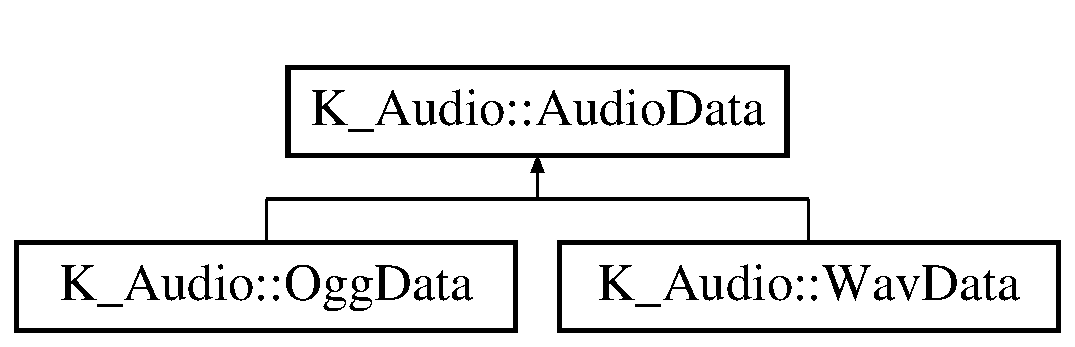
\includegraphics[height=2.000000cm]{class_k___audio_1_1_audio_data}
\end{center}
\end{figure}
\subsection*{公開型}
\begin{DoxyCompactItemize}
\item 
enum \mbox{\hyperlink{class_k___audio_1_1_audio_data_a7ef9acd4f7d2140951605d835cff2435}{Sound\+Format}} \{ \mbox{\hyperlink{class_k___audio_1_1_audio_data_a7ef9acd4f7d2140951605d835cff2435a9cfb443c5ead7e17f06e768eb2a9e915}{Mono8}}, 
\mbox{\hyperlink{class_k___audio_1_1_audio_data_a7ef9acd4f7d2140951605d835cff2435ad51581c07626d73329902c1587893768}{Mono16}}, 
\mbox{\hyperlink{class_k___audio_1_1_audio_data_a7ef9acd4f7d2140951605d835cff2435aecf057ba8d0fde7613a07aa0be0fcd3b}{Stereo8}}, 
\mbox{\hyperlink{class_k___audio_1_1_audio_data_a7ef9acd4f7d2140951605d835cff2435a4ebe72d0f83b3fc18973504a68c63f65}{Stereo16}}
 \}
\begin{DoxyCompactList}\small\item\em サウンド形式列挙型、数字はビット数を表す \end{DoxyCompactList}\end{DoxyCompactItemize}
\subsection*{公開メンバ関数}
\begin{DoxyCompactItemize}
\item 
\mbox{\hyperlink{class_k___audio_1_1_audio_data_a78c3668af550d54e5a16e5658afc4ec8}{Audio\+Data}} ()
\item 
virtual \mbox{\hyperlink{class_k___audio_1_1_audio_data_aebb74e1d7096a4580497da2bd72c019c}{$\sim$\+Audio\+Data}} ()
\item 
virtual bool \mbox{\hyperlink{class_k___audio_1_1_audio_data_a97453a72c7161214868303f6fdca9494}{Load\+File}} (const char $\ast$file\+Pass)=0
\item 
virtual int \mbox{\hyperlink{class_k___audio_1_1_audio_data_af42b123ad2ce45867401d697fd572392}{Read}} (char $\ast$buffer, int max\+Size)=0
\item 
virtual void \mbox{\hyperlink{class_k___audio_1_1_audio_data_a1ba3ab1b4bae0b460d26278cb29ce16e}{Seek}} (int \mbox{\hyperlink{class_k___audio_1_1_audio_data_a8c1a6d96d9c2c55467baf9c0e7e58c98}{pcm\+Offset}})=0
\item 
virtual int \mbox{\hyperlink{class_k___audio_1_1_audio_data_ae075eaedf3a552c083d0ed7e0c24fdce}{Get\+Pcm\+Offset}} ()
\item 
virtual int \mbox{\hyperlink{class_k___audio_1_1_audio_data_a94740233be10a58fba516fe6ae0aaa3a}{Get\+Loop\+Start}} ()
\item 
virtual int \mbox{\hyperlink{class_k___audio_1_1_audio_data_ae29cd0dcfcd55a12d6279f4b95956f1b}{Get\+Loop\+Length}} ()
\item 
virtual int \mbox{\hyperlink{class_k___audio_1_1_audio_data_ac44af4a5c1cecb476fff9faa2cab64b8}{Get\+Pcm\+Size}} ()
\item 
virtual int \mbox{\hyperlink{class_k___audio_1_1_audio_data_a2a5e7bf50936f9974a4e6f07bdb45037}{Get\+Block\+Size}} ()
\item 
virtual \mbox{\hyperlink{class_k___audio_1_1_audio_data_a7ef9acd4f7d2140951605d835cff2435}{Sound\+Format}} \mbox{\hyperlink{class_k___audio_1_1_audio_data_a7d2e29b72ce32c6b733b856b59d38492}{Get\+Format}} ()
\item 
virtual int \mbox{\hyperlink{class_k___audio_1_1_audio_data_a52ca0190e77d44e12ca222a7eb1b5e84}{Get\+Sampling\+Rate}} ()
\end{DoxyCompactItemize}
\subsection*{限定公開変数類}
\begin{DoxyCompactItemize}
\item 
int \mbox{\hyperlink{class_k___audio_1_1_audio_data_a2d6bf30ca113346be54ac45e1ffcd05a}{pcm\+Size}}
\item 
int \mbox{\hyperlink{class_k___audio_1_1_audio_data_a8c1a6d96d9c2c55467baf9c0e7e58c98}{pcm\+Offset}}
\item 
int \mbox{\hyperlink{class_k___audio_1_1_audio_data_a94a2c5cc216653a4928e86953c03d0ba}{loop\+Start}}
\item 
int \mbox{\hyperlink{class_k___audio_1_1_audio_data_aeeeb3e8ef6215672507749088fe41266}{loop\+Length}}
\item 
\mbox{\hyperlink{class_k___audio_1_1_audio_data_a7ef9acd4f7d2140951605d835cff2435}{Sound\+Format}} \mbox{\hyperlink{class_k___audio_1_1_audio_data_a9dc7fef30a3ca815a829c1009a6ecc33}{format}}
\item 
int \mbox{\hyperlink{class_k___audio_1_1_audio_data_a6730a05b5833bbbeb5512d28a09df9ff}{sampling\+Rate}}
\item 
int \mbox{\hyperlink{class_k___audio_1_1_audio_data_a8e8445d5d8449b7b7bbafeaf893bad74}{block\+Size}}
\end{DoxyCompactItemize}


\subsection{列挙型メンバ詳解}
\mbox{\Hypertarget{class_k___audio_1_1_audio_data_a7ef9acd4f7d2140951605d835cff2435}\label{class_k___audio_1_1_audio_data_a7ef9acd4f7d2140951605d835cff2435}} 
\index{K\+\_\+\+Audio\+::\+Audio\+Data@{K\+\_\+\+Audio\+::\+Audio\+Data}!Sound\+Format@{Sound\+Format}}
\index{Sound\+Format@{Sound\+Format}!K\+\_\+\+Audio\+::\+Audio\+Data@{K\+\_\+\+Audio\+::\+Audio\+Data}}
\subsubsection{\texorpdfstring{Sound\+Format}{SoundFormat}}
{\footnotesize\ttfamily enum \mbox{\hyperlink{class_k___audio_1_1_audio_data_a7ef9acd4f7d2140951605d835cff2435}{K\+\_\+\+Audio\+::\+Audio\+Data\+::\+Sound\+Format}}}



サウンド形式列挙型、数字はビット数を表す 

\begin{DoxyEnumFields}{列挙値}
\raisebox{\heightof{T}}[0pt][0pt]{\index{Mono8@{Mono8}!K\+\_\+\+Audio\+::\+Audio\+Data@{K\+\_\+\+Audio\+::\+Audio\+Data}}\index{K\+\_\+\+Audio\+::\+Audio\+Data@{K\+\_\+\+Audio\+::\+Audio\+Data}!Mono8@{Mono8}}}\mbox{\Hypertarget{class_k___audio_1_1_audio_data_a7ef9acd4f7d2140951605d835cff2435a9cfb443c5ead7e17f06e768eb2a9e915}\label{class_k___audio_1_1_audio_data_a7ef9acd4f7d2140951605d835cff2435a9cfb443c5ead7e17f06e768eb2a9e915}} 
Mono8&\\
\hline

\raisebox{\heightof{T}}[0pt][0pt]{\index{Mono16@{Mono16}!K\+\_\+\+Audio\+::\+Audio\+Data@{K\+\_\+\+Audio\+::\+Audio\+Data}}\index{K\+\_\+\+Audio\+::\+Audio\+Data@{K\+\_\+\+Audio\+::\+Audio\+Data}!Mono16@{Mono16}}}\mbox{\Hypertarget{class_k___audio_1_1_audio_data_a7ef9acd4f7d2140951605d835cff2435ad51581c07626d73329902c1587893768}\label{class_k___audio_1_1_audio_data_a7ef9acd4f7d2140951605d835cff2435ad51581c07626d73329902c1587893768}} 
Mono16&\\
\hline

\raisebox{\heightof{T}}[0pt][0pt]{\index{Stereo8@{Stereo8}!K\+\_\+\+Audio\+::\+Audio\+Data@{K\+\_\+\+Audio\+::\+Audio\+Data}}\index{K\+\_\+\+Audio\+::\+Audio\+Data@{K\+\_\+\+Audio\+::\+Audio\+Data}!Stereo8@{Stereo8}}}\mbox{\Hypertarget{class_k___audio_1_1_audio_data_a7ef9acd4f7d2140951605d835cff2435aecf057ba8d0fde7613a07aa0be0fcd3b}\label{class_k___audio_1_1_audio_data_a7ef9acd4f7d2140951605d835cff2435aecf057ba8d0fde7613a07aa0be0fcd3b}} 
Stereo8&\\
\hline

\raisebox{\heightof{T}}[0pt][0pt]{\index{Stereo16@{Stereo16}!K\+\_\+\+Audio\+::\+Audio\+Data@{K\+\_\+\+Audio\+::\+Audio\+Data}}\index{K\+\_\+\+Audio\+::\+Audio\+Data@{K\+\_\+\+Audio\+::\+Audio\+Data}!Stereo16@{Stereo16}}}\mbox{\Hypertarget{class_k___audio_1_1_audio_data_a7ef9acd4f7d2140951605d835cff2435a4ebe72d0f83b3fc18973504a68c63f65}\label{class_k___audio_1_1_audio_data_a7ef9acd4f7d2140951605d835cff2435a4ebe72d0f83b3fc18973504a68c63f65}} 
Stereo16&\\
\hline

\end{DoxyEnumFields}


\subsection{構築子と解体子}
\mbox{\Hypertarget{class_k___audio_1_1_audio_data_a78c3668af550d54e5a16e5658afc4ec8}\label{class_k___audio_1_1_audio_data_a78c3668af550d54e5a16e5658afc4ec8}} 
\index{K\+\_\+\+Audio\+::\+Audio\+Data@{K\+\_\+\+Audio\+::\+Audio\+Data}!Audio\+Data@{Audio\+Data}}
\index{Audio\+Data@{Audio\+Data}!K\+\_\+\+Audio\+::\+Audio\+Data@{K\+\_\+\+Audio\+::\+Audio\+Data}}
\subsubsection{\texorpdfstring{Audio\+Data()}{AudioData()}}
{\footnotesize\ttfamily K\+\_\+\+Audio\+::\+Audio\+Data\+::\+Audio\+Data (\begin{DoxyParamCaption}{ }\end{DoxyParamCaption})}

\mbox{\Hypertarget{class_k___audio_1_1_audio_data_aebb74e1d7096a4580497da2bd72c019c}\label{class_k___audio_1_1_audio_data_aebb74e1d7096a4580497da2bd72c019c}} 
\index{K\+\_\+\+Audio\+::\+Audio\+Data@{K\+\_\+\+Audio\+::\+Audio\+Data}!````~Audio\+Data@{$\sim$\+Audio\+Data}}
\index{````~Audio\+Data@{$\sim$\+Audio\+Data}!K\+\_\+\+Audio\+::\+Audio\+Data@{K\+\_\+\+Audio\+::\+Audio\+Data}}
\subsubsection{\texorpdfstring{$\sim$\+Audio\+Data()}{~AudioData()}}
{\footnotesize\ttfamily virtual K\+\_\+\+Audio\+::\+Audio\+Data\+::$\sim$\+Audio\+Data (\begin{DoxyParamCaption}{ }\end{DoxyParamCaption})\hspace{0.3cm}{\ttfamily [virtual]}}



\subsection{関数詳解}
\mbox{\Hypertarget{class_k___audio_1_1_audio_data_a2a5e7bf50936f9974a4e6f07bdb45037}\label{class_k___audio_1_1_audio_data_a2a5e7bf50936f9974a4e6f07bdb45037}} 
\index{K\+\_\+\+Audio\+::\+Audio\+Data@{K\+\_\+\+Audio\+::\+Audio\+Data}!Get\+Block\+Size@{Get\+Block\+Size}}
\index{Get\+Block\+Size@{Get\+Block\+Size}!K\+\_\+\+Audio\+::\+Audio\+Data@{K\+\_\+\+Audio\+::\+Audio\+Data}}
\subsubsection{\texorpdfstring{Get\+Block\+Size()}{GetBlockSize()}}
{\footnotesize\ttfamily virtual int K\+\_\+\+Audio\+::\+Audio\+Data\+::\+Get\+Block\+Size (\begin{DoxyParamCaption}{ }\end{DoxyParamCaption})\hspace{0.3cm}{\ttfamily [virtual]}}

\mbox{\Hypertarget{class_k___audio_1_1_audio_data_a7d2e29b72ce32c6b733b856b59d38492}\label{class_k___audio_1_1_audio_data_a7d2e29b72ce32c6b733b856b59d38492}} 
\index{K\+\_\+\+Audio\+::\+Audio\+Data@{K\+\_\+\+Audio\+::\+Audio\+Data}!Get\+Format@{Get\+Format}}
\index{Get\+Format@{Get\+Format}!K\+\_\+\+Audio\+::\+Audio\+Data@{K\+\_\+\+Audio\+::\+Audio\+Data}}
\subsubsection{\texorpdfstring{Get\+Format()}{GetFormat()}}
{\footnotesize\ttfamily virtual \mbox{\hyperlink{class_k___audio_1_1_audio_data_a7ef9acd4f7d2140951605d835cff2435}{Sound\+Format}} K\+\_\+\+Audio\+::\+Audio\+Data\+::\+Get\+Format (\begin{DoxyParamCaption}{ }\end{DoxyParamCaption})\hspace{0.3cm}{\ttfamily [virtual]}}

\mbox{\Hypertarget{class_k___audio_1_1_audio_data_ae29cd0dcfcd55a12d6279f4b95956f1b}\label{class_k___audio_1_1_audio_data_ae29cd0dcfcd55a12d6279f4b95956f1b}} 
\index{K\+\_\+\+Audio\+::\+Audio\+Data@{K\+\_\+\+Audio\+::\+Audio\+Data}!Get\+Loop\+Length@{Get\+Loop\+Length}}
\index{Get\+Loop\+Length@{Get\+Loop\+Length}!K\+\_\+\+Audio\+::\+Audio\+Data@{K\+\_\+\+Audio\+::\+Audio\+Data}}
\subsubsection{\texorpdfstring{Get\+Loop\+Length()}{GetLoopLength()}}
{\footnotesize\ttfamily virtual int K\+\_\+\+Audio\+::\+Audio\+Data\+::\+Get\+Loop\+Length (\begin{DoxyParamCaption}{ }\end{DoxyParamCaption})\hspace{0.3cm}{\ttfamily [virtual]}}

\mbox{\Hypertarget{class_k___audio_1_1_audio_data_a94740233be10a58fba516fe6ae0aaa3a}\label{class_k___audio_1_1_audio_data_a94740233be10a58fba516fe6ae0aaa3a}} 
\index{K\+\_\+\+Audio\+::\+Audio\+Data@{K\+\_\+\+Audio\+::\+Audio\+Data}!Get\+Loop\+Start@{Get\+Loop\+Start}}
\index{Get\+Loop\+Start@{Get\+Loop\+Start}!K\+\_\+\+Audio\+::\+Audio\+Data@{K\+\_\+\+Audio\+::\+Audio\+Data}}
\subsubsection{\texorpdfstring{Get\+Loop\+Start()}{GetLoopStart()}}
{\footnotesize\ttfamily virtual int K\+\_\+\+Audio\+::\+Audio\+Data\+::\+Get\+Loop\+Start (\begin{DoxyParamCaption}{ }\end{DoxyParamCaption})\hspace{0.3cm}{\ttfamily [virtual]}}

\mbox{\Hypertarget{class_k___audio_1_1_audio_data_ae075eaedf3a552c083d0ed7e0c24fdce}\label{class_k___audio_1_1_audio_data_ae075eaedf3a552c083d0ed7e0c24fdce}} 
\index{K\+\_\+\+Audio\+::\+Audio\+Data@{K\+\_\+\+Audio\+::\+Audio\+Data}!Get\+Pcm\+Offset@{Get\+Pcm\+Offset}}
\index{Get\+Pcm\+Offset@{Get\+Pcm\+Offset}!K\+\_\+\+Audio\+::\+Audio\+Data@{K\+\_\+\+Audio\+::\+Audio\+Data}}
\subsubsection{\texorpdfstring{Get\+Pcm\+Offset()}{GetPcmOffset()}}
{\footnotesize\ttfamily virtual int K\+\_\+\+Audio\+::\+Audio\+Data\+::\+Get\+Pcm\+Offset (\begin{DoxyParamCaption}{ }\end{DoxyParamCaption})\hspace{0.3cm}{\ttfamily [virtual]}}

\mbox{\Hypertarget{class_k___audio_1_1_audio_data_ac44af4a5c1cecb476fff9faa2cab64b8}\label{class_k___audio_1_1_audio_data_ac44af4a5c1cecb476fff9faa2cab64b8}} 
\index{K\+\_\+\+Audio\+::\+Audio\+Data@{K\+\_\+\+Audio\+::\+Audio\+Data}!Get\+Pcm\+Size@{Get\+Pcm\+Size}}
\index{Get\+Pcm\+Size@{Get\+Pcm\+Size}!K\+\_\+\+Audio\+::\+Audio\+Data@{K\+\_\+\+Audio\+::\+Audio\+Data}}
\subsubsection{\texorpdfstring{Get\+Pcm\+Size()}{GetPcmSize()}}
{\footnotesize\ttfamily virtual int K\+\_\+\+Audio\+::\+Audio\+Data\+::\+Get\+Pcm\+Size (\begin{DoxyParamCaption}{ }\end{DoxyParamCaption})\hspace{0.3cm}{\ttfamily [virtual]}}

\mbox{\Hypertarget{class_k___audio_1_1_audio_data_a52ca0190e77d44e12ca222a7eb1b5e84}\label{class_k___audio_1_1_audio_data_a52ca0190e77d44e12ca222a7eb1b5e84}} 
\index{K\+\_\+\+Audio\+::\+Audio\+Data@{K\+\_\+\+Audio\+::\+Audio\+Data}!Get\+Sampling\+Rate@{Get\+Sampling\+Rate}}
\index{Get\+Sampling\+Rate@{Get\+Sampling\+Rate}!K\+\_\+\+Audio\+::\+Audio\+Data@{K\+\_\+\+Audio\+::\+Audio\+Data}}
\subsubsection{\texorpdfstring{Get\+Sampling\+Rate()}{GetSamplingRate()}}
{\footnotesize\ttfamily virtual int K\+\_\+\+Audio\+::\+Audio\+Data\+::\+Get\+Sampling\+Rate (\begin{DoxyParamCaption}{ }\end{DoxyParamCaption})\hspace{0.3cm}{\ttfamily [virtual]}}

\mbox{\Hypertarget{class_k___audio_1_1_audio_data_a97453a72c7161214868303f6fdca9494}\label{class_k___audio_1_1_audio_data_a97453a72c7161214868303f6fdca9494}} 
\index{K\+\_\+\+Audio\+::\+Audio\+Data@{K\+\_\+\+Audio\+::\+Audio\+Data}!Load\+File@{Load\+File}}
\index{Load\+File@{Load\+File}!K\+\_\+\+Audio\+::\+Audio\+Data@{K\+\_\+\+Audio\+::\+Audio\+Data}}
\subsubsection{\texorpdfstring{Load\+File()}{LoadFile()}}
{\footnotesize\ttfamily virtual bool K\+\_\+\+Audio\+::\+Audio\+Data\+::\+Load\+File (\begin{DoxyParamCaption}\item[{const char $\ast$}]{file\+Pass }\end{DoxyParamCaption})\hspace{0.3cm}{\ttfamily [pure virtual]}}

\mbox{\Hypertarget{class_k___audio_1_1_audio_data_af42b123ad2ce45867401d697fd572392}\label{class_k___audio_1_1_audio_data_af42b123ad2ce45867401d697fd572392}} 
\index{K\+\_\+\+Audio\+::\+Audio\+Data@{K\+\_\+\+Audio\+::\+Audio\+Data}!Read@{Read}}
\index{Read@{Read}!K\+\_\+\+Audio\+::\+Audio\+Data@{K\+\_\+\+Audio\+::\+Audio\+Data}}
\subsubsection{\texorpdfstring{Read()}{Read()}}
{\footnotesize\ttfamily virtual int K\+\_\+\+Audio\+::\+Audio\+Data\+::\+Read (\begin{DoxyParamCaption}\item[{char $\ast$}]{buffer,  }\item[{int}]{max\+Size }\end{DoxyParamCaption})\hspace{0.3cm}{\ttfamily [pure virtual]}}



\mbox{\hyperlink{class_k___audio_1_1_wav_data_a9b64967d83ac218c71949335d0583e69}{K\+\_\+\+Audio\+::\+Wav\+Data}}, \mbox{\hyperlink{class_k___audio_1_1_ogg_data_ac4c50916e0f2eaa384539b2dbedc1d6e}{K\+\_\+\+Audio\+::\+Ogg\+Data}}で実装されています。

\mbox{\Hypertarget{class_k___audio_1_1_audio_data_a1ba3ab1b4bae0b460d26278cb29ce16e}\label{class_k___audio_1_1_audio_data_a1ba3ab1b4bae0b460d26278cb29ce16e}} 
\index{K\+\_\+\+Audio\+::\+Audio\+Data@{K\+\_\+\+Audio\+::\+Audio\+Data}!Seek@{Seek}}
\index{Seek@{Seek}!K\+\_\+\+Audio\+::\+Audio\+Data@{K\+\_\+\+Audio\+::\+Audio\+Data}}
\subsubsection{\texorpdfstring{Seek()}{Seek()}}
{\footnotesize\ttfamily virtual void K\+\_\+\+Audio\+::\+Audio\+Data\+::\+Seek (\begin{DoxyParamCaption}\item[{int}]{pcm\+Offset }\end{DoxyParamCaption})\hspace{0.3cm}{\ttfamily [pure virtual]}}



\mbox{\hyperlink{class_k___audio_1_1_wav_data_a2af2d93fb22fe25a4739c2b40526a7af}{K\+\_\+\+Audio\+::\+Wav\+Data}}, \mbox{\hyperlink{class_k___audio_1_1_ogg_data_aac0e955981398bf31053f27fbe19b2ba}{K\+\_\+\+Audio\+::\+Ogg\+Data}}で実装されています。



\subsection{メンバ詳解}
\mbox{\Hypertarget{class_k___audio_1_1_audio_data_a8e8445d5d8449b7b7bbafeaf893bad74}\label{class_k___audio_1_1_audio_data_a8e8445d5d8449b7b7bbafeaf893bad74}} 
\index{K\+\_\+\+Audio\+::\+Audio\+Data@{K\+\_\+\+Audio\+::\+Audio\+Data}!block\+Size@{block\+Size}}
\index{block\+Size@{block\+Size}!K\+\_\+\+Audio\+::\+Audio\+Data@{K\+\_\+\+Audio\+::\+Audio\+Data}}
\subsubsection{\texorpdfstring{block\+Size}{blockSize}}
{\footnotesize\ttfamily int K\+\_\+\+Audio\+::\+Audio\+Data\+::block\+Size\hspace{0.3cm}{\ttfamily [protected]}}

\mbox{\Hypertarget{class_k___audio_1_1_audio_data_a9dc7fef30a3ca815a829c1009a6ecc33}\label{class_k___audio_1_1_audio_data_a9dc7fef30a3ca815a829c1009a6ecc33}} 
\index{K\+\_\+\+Audio\+::\+Audio\+Data@{K\+\_\+\+Audio\+::\+Audio\+Data}!format@{format}}
\index{format@{format}!K\+\_\+\+Audio\+::\+Audio\+Data@{K\+\_\+\+Audio\+::\+Audio\+Data}}
\subsubsection{\texorpdfstring{format}{format}}
{\footnotesize\ttfamily \mbox{\hyperlink{class_k___audio_1_1_audio_data_a7ef9acd4f7d2140951605d835cff2435}{Sound\+Format}} K\+\_\+\+Audio\+::\+Audio\+Data\+::format\hspace{0.3cm}{\ttfamily [protected]}}

\mbox{\Hypertarget{class_k___audio_1_1_audio_data_aeeeb3e8ef6215672507749088fe41266}\label{class_k___audio_1_1_audio_data_aeeeb3e8ef6215672507749088fe41266}} 
\index{K\+\_\+\+Audio\+::\+Audio\+Data@{K\+\_\+\+Audio\+::\+Audio\+Data}!loop\+Length@{loop\+Length}}
\index{loop\+Length@{loop\+Length}!K\+\_\+\+Audio\+::\+Audio\+Data@{K\+\_\+\+Audio\+::\+Audio\+Data}}
\subsubsection{\texorpdfstring{loop\+Length}{loopLength}}
{\footnotesize\ttfamily int K\+\_\+\+Audio\+::\+Audio\+Data\+::loop\+Length\hspace{0.3cm}{\ttfamily [protected]}}

\mbox{\Hypertarget{class_k___audio_1_1_audio_data_a94a2c5cc216653a4928e86953c03d0ba}\label{class_k___audio_1_1_audio_data_a94a2c5cc216653a4928e86953c03d0ba}} 
\index{K\+\_\+\+Audio\+::\+Audio\+Data@{K\+\_\+\+Audio\+::\+Audio\+Data}!loop\+Start@{loop\+Start}}
\index{loop\+Start@{loop\+Start}!K\+\_\+\+Audio\+::\+Audio\+Data@{K\+\_\+\+Audio\+::\+Audio\+Data}}
\subsubsection{\texorpdfstring{loop\+Start}{loopStart}}
{\footnotesize\ttfamily int K\+\_\+\+Audio\+::\+Audio\+Data\+::loop\+Start\hspace{0.3cm}{\ttfamily [protected]}}

\mbox{\Hypertarget{class_k___audio_1_1_audio_data_a8c1a6d96d9c2c55467baf9c0e7e58c98}\label{class_k___audio_1_1_audio_data_a8c1a6d96d9c2c55467baf9c0e7e58c98}} 
\index{K\+\_\+\+Audio\+::\+Audio\+Data@{K\+\_\+\+Audio\+::\+Audio\+Data}!pcm\+Offset@{pcm\+Offset}}
\index{pcm\+Offset@{pcm\+Offset}!K\+\_\+\+Audio\+::\+Audio\+Data@{K\+\_\+\+Audio\+::\+Audio\+Data}}
\subsubsection{\texorpdfstring{pcm\+Offset}{pcmOffset}}
{\footnotesize\ttfamily int K\+\_\+\+Audio\+::\+Audio\+Data\+::pcm\+Offset\hspace{0.3cm}{\ttfamily [protected]}}

\mbox{\Hypertarget{class_k___audio_1_1_audio_data_a2d6bf30ca113346be54ac45e1ffcd05a}\label{class_k___audio_1_1_audio_data_a2d6bf30ca113346be54ac45e1ffcd05a}} 
\index{K\+\_\+\+Audio\+::\+Audio\+Data@{K\+\_\+\+Audio\+::\+Audio\+Data}!pcm\+Size@{pcm\+Size}}
\index{pcm\+Size@{pcm\+Size}!K\+\_\+\+Audio\+::\+Audio\+Data@{K\+\_\+\+Audio\+::\+Audio\+Data}}
\subsubsection{\texorpdfstring{pcm\+Size}{pcmSize}}
{\footnotesize\ttfamily int K\+\_\+\+Audio\+::\+Audio\+Data\+::pcm\+Size\hspace{0.3cm}{\ttfamily [protected]}}

\mbox{\Hypertarget{class_k___audio_1_1_audio_data_a6730a05b5833bbbeb5512d28a09df9ff}\label{class_k___audio_1_1_audio_data_a6730a05b5833bbbeb5512d28a09df9ff}} 
\index{K\+\_\+\+Audio\+::\+Audio\+Data@{K\+\_\+\+Audio\+::\+Audio\+Data}!sampling\+Rate@{sampling\+Rate}}
\index{sampling\+Rate@{sampling\+Rate}!K\+\_\+\+Audio\+::\+Audio\+Data@{K\+\_\+\+Audio\+::\+Audio\+Data}}
\subsubsection{\texorpdfstring{sampling\+Rate}{samplingRate}}
{\footnotesize\ttfamily int K\+\_\+\+Audio\+::\+Audio\+Data\+::sampling\+Rate\hspace{0.3cm}{\ttfamily [protected]}}


\hypertarget{class_k___audio_1_1_audio_data_factory}{}\section{K\+\_\+\+Audio\+:\+:Audio\+Data\+Factory クラス}
\label{class_k___audio_1_1_audio_data_factory}\index{K\+\_\+\+Audio\+::\+Audio\+Data\+Factory@{K\+\_\+\+Audio\+::\+Audio\+Data\+Factory}}


{\ttfamily \#include $<$Audio\+Data\+Factory.\+h$>$}

\subsection*{公開型}
\begin{DoxyCompactItemize}
\item 
enum \mbox{\hyperlink{class_k___audio_1_1_audio_data_factory_a070a4d999e204c8c78cd9f16a1c732ea}{Audio\+Type}} \{ \mbox{\hyperlink{class_k___audio_1_1_audio_data_factory_a070a4d999e204c8c78cd9f16a1c732eaac50f7a3cb913ee2eb98fe1664b442f6b}{Wave}}, 
\mbox{\hyperlink{class_k___audio_1_1_audio_data_factory_a070a4d999e204c8c78cd9f16a1c732eaac4e902b17eee79a21d1ab0550fb152be}{Ogg}}, 
\mbox{\hyperlink{class_k___audio_1_1_audio_data_factory_a070a4d999e204c8c78cd9f16a1c732eaab27c3fa7a2eb8cd78b05809b36596e10}{Non\+Support}}
 \}
\end{DoxyCompactItemize}
\subsection*{公開メンバ関数}
\begin{DoxyCompactItemize}
\item 
\mbox{\hyperlink{class_k___audio_1_1_audio_data_factory_a13e01c1708127344b0f8b44b27b847e0}{Audio\+Data\+Factory}} ()
\item 
\mbox{\hyperlink{class_k___audio_1_1_audio_data_factory_a922d66a38fbf21340c291283487388da}{$\sim$\+Audio\+Data\+Factory}} ()
\item 
\mbox{\hyperlink{class_k___audio_1_1_audio_data}{Audio\+Data}} $\ast$ \mbox{\hyperlink{class_k___audio_1_1_audio_data_factory_a2ab1886d205b300e8255b153ded7ffcb}{Create}} (const char $\ast$file\+Pass)
\end{DoxyCompactItemize}


\subsection{列挙型メンバ詳解}
\mbox{\Hypertarget{class_k___audio_1_1_audio_data_factory_a070a4d999e204c8c78cd9f16a1c732ea}\label{class_k___audio_1_1_audio_data_factory_a070a4d999e204c8c78cd9f16a1c732ea}} 
\index{K\+\_\+\+Audio\+::\+Audio\+Data\+Factory@{K\+\_\+\+Audio\+::\+Audio\+Data\+Factory}!Audio\+Type@{Audio\+Type}}
\index{Audio\+Type@{Audio\+Type}!K\+\_\+\+Audio\+::\+Audio\+Data\+Factory@{K\+\_\+\+Audio\+::\+Audio\+Data\+Factory}}
\subsubsection{\texorpdfstring{Audio\+Type}{AudioType}}
{\footnotesize\ttfamily enum \mbox{\hyperlink{class_k___audio_1_1_audio_data_factory_a070a4d999e204c8c78cd9f16a1c732ea}{K\+\_\+\+Audio\+::\+Audio\+Data\+Factory\+::\+Audio\+Type}}}

\begin{DoxyEnumFields}{列挙値}
\raisebox{\heightof{T}}[0pt][0pt]{\index{Wave@{Wave}!K\+\_\+\+Audio\+::\+Audio\+Data\+Factory@{K\+\_\+\+Audio\+::\+Audio\+Data\+Factory}}\index{K\+\_\+\+Audio\+::\+Audio\+Data\+Factory@{K\+\_\+\+Audio\+::\+Audio\+Data\+Factory}!Wave@{Wave}}}\mbox{\Hypertarget{class_k___audio_1_1_audio_data_factory_a070a4d999e204c8c78cd9f16a1c732eaac50f7a3cb913ee2eb98fe1664b442f6b}\label{class_k___audio_1_1_audio_data_factory_a070a4d999e204c8c78cd9f16a1c732eaac50f7a3cb913ee2eb98fe1664b442f6b}} 
Wave&\\
\hline

\raisebox{\heightof{T}}[0pt][0pt]{\index{Ogg@{Ogg}!K\+\_\+\+Audio\+::\+Audio\+Data\+Factory@{K\+\_\+\+Audio\+::\+Audio\+Data\+Factory}}\index{K\+\_\+\+Audio\+::\+Audio\+Data\+Factory@{K\+\_\+\+Audio\+::\+Audio\+Data\+Factory}!Ogg@{Ogg}}}\mbox{\Hypertarget{class_k___audio_1_1_audio_data_factory_a070a4d999e204c8c78cd9f16a1c732eaac4e902b17eee79a21d1ab0550fb152be}\label{class_k___audio_1_1_audio_data_factory_a070a4d999e204c8c78cd9f16a1c732eaac4e902b17eee79a21d1ab0550fb152be}} 
Ogg&\\
\hline

\raisebox{\heightof{T}}[0pt][0pt]{\index{Non\+Support@{Non\+Support}!K\+\_\+\+Audio\+::\+Audio\+Data\+Factory@{K\+\_\+\+Audio\+::\+Audio\+Data\+Factory}}\index{K\+\_\+\+Audio\+::\+Audio\+Data\+Factory@{K\+\_\+\+Audio\+::\+Audio\+Data\+Factory}!Non\+Support@{Non\+Support}}}\mbox{\Hypertarget{class_k___audio_1_1_audio_data_factory_a070a4d999e204c8c78cd9f16a1c732eaab27c3fa7a2eb8cd78b05809b36596e10}\label{class_k___audio_1_1_audio_data_factory_a070a4d999e204c8c78cd9f16a1c732eaab27c3fa7a2eb8cd78b05809b36596e10}} 
Non\+Support&\\
\hline

\end{DoxyEnumFields}


\subsection{構築子と解体子}
\mbox{\Hypertarget{class_k___audio_1_1_audio_data_factory_a13e01c1708127344b0f8b44b27b847e0}\label{class_k___audio_1_1_audio_data_factory_a13e01c1708127344b0f8b44b27b847e0}} 
\index{K\+\_\+\+Audio\+::\+Audio\+Data\+Factory@{K\+\_\+\+Audio\+::\+Audio\+Data\+Factory}!Audio\+Data\+Factory@{Audio\+Data\+Factory}}
\index{Audio\+Data\+Factory@{Audio\+Data\+Factory}!K\+\_\+\+Audio\+::\+Audio\+Data\+Factory@{K\+\_\+\+Audio\+::\+Audio\+Data\+Factory}}
\subsubsection{\texorpdfstring{Audio\+Data\+Factory()}{AudioDataFactory()}}
{\footnotesize\ttfamily K\+\_\+\+Audio\+::\+Audio\+Data\+Factory\+::\+Audio\+Data\+Factory (\begin{DoxyParamCaption}{ }\end{DoxyParamCaption})}

\mbox{\Hypertarget{class_k___audio_1_1_audio_data_factory_a922d66a38fbf21340c291283487388da}\label{class_k___audio_1_1_audio_data_factory_a922d66a38fbf21340c291283487388da}} 
\index{K\+\_\+\+Audio\+::\+Audio\+Data\+Factory@{K\+\_\+\+Audio\+::\+Audio\+Data\+Factory}!````~Audio\+Data\+Factory@{$\sim$\+Audio\+Data\+Factory}}
\index{````~Audio\+Data\+Factory@{$\sim$\+Audio\+Data\+Factory}!K\+\_\+\+Audio\+::\+Audio\+Data\+Factory@{K\+\_\+\+Audio\+::\+Audio\+Data\+Factory}}
\subsubsection{\texorpdfstring{$\sim$\+Audio\+Data\+Factory()}{~AudioDataFactory()}}
{\footnotesize\ttfamily K\+\_\+\+Audio\+::\+Audio\+Data\+Factory\+::$\sim$\+Audio\+Data\+Factory (\begin{DoxyParamCaption}{ }\end{DoxyParamCaption})}



\subsection{関数詳解}
\mbox{\Hypertarget{class_k___audio_1_1_audio_data_factory_a2ab1886d205b300e8255b153ded7ffcb}\label{class_k___audio_1_1_audio_data_factory_a2ab1886d205b300e8255b153ded7ffcb}} 
\index{K\+\_\+\+Audio\+::\+Audio\+Data\+Factory@{K\+\_\+\+Audio\+::\+Audio\+Data\+Factory}!Create@{Create}}
\index{Create@{Create}!K\+\_\+\+Audio\+::\+Audio\+Data\+Factory@{K\+\_\+\+Audio\+::\+Audio\+Data\+Factory}}
\subsubsection{\texorpdfstring{Create()}{Create()}}
{\footnotesize\ttfamily \mbox{\hyperlink{class_k___audio_1_1_audio_data}{Audio\+Data}}$\ast$ K\+\_\+\+Audio\+::\+Audio\+Data\+Factory\+::\+Create (\begin{DoxyParamCaption}\item[{const char $\ast$}]{file\+Pass }\end{DoxyParamCaption})}


\hypertarget{struct_k___input_1_1_axis_state}{}\section{K\+\_\+\+Input\+:\+:Axis\+State 構造体}
\label{struct_k___input_1_1_axis_state}\index{K\+\_\+\+Input\+::\+Axis\+State@{K\+\_\+\+Input\+::\+Axis\+State}}


アナログスティックの軸  




{\ttfamily \#include $<$Vpad\+States.\+h$>$}

\subsection*{公開変数類}
\begin{DoxyCompactItemize}
\item 
\mbox{\hyperlink{namespace_k___input_a82230ae06723a21cc710ae3d66fd078f}{Joy\+Axis}} \mbox{\hyperlink{struct_k___input_1_1_axis_state_a253890a432ae112fc57d39f7e06c88ad}{axis}}
\item 
\mbox{\hyperlink{namespace_k___input_af62d80c77b12db01035e4b9aa27a09d6}{Key}} \mbox{\hyperlink{struct_k___input_1_1_axis_state_ad652895e754dfc2be58995677bf97ec6}{plus\+Button}}
\item 
\mbox{\hyperlink{namespace_k___input_af62d80c77b12db01035e4b9aa27a09d6}{Key}} \mbox{\hyperlink{struct_k___input_1_1_axis_state_ad1c843ecba70aa4035dfe71c498b26c1}{minus\+Button}}
\item 
float \mbox{\hyperlink{struct_k___input_1_1_axis_state_ac23cfe9122fca5a53ca24fcacb3f2123}{pos}}
\end{DoxyCompactItemize}


\subsection{詳解}
アナログスティックの軸 

\subsection{メンバ詳解}
\mbox{\Hypertarget{struct_k___input_1_1_axis_state_a253890a432ae112fc57d39f7e06c88ad}\label{struct_k___input_1_1_axis_state_a253890a432ae112fc57d39f7e06c88ad}} 
\index{K\+\_\+\+Input\+::\+Axis\+State@{K\+\_\+\+Input\+::\+Axis\+State}!axis@{axis}}
\index{axis@{axis}!K\+\_\+\+Input\+::\+Axis\+State@{K\+\_\+\+Input\+::\+Axis\+State}}
\subsubsection{\texorpdfstring{axis}{axis}}
{\footnotesize\ttfamily \mbox{\hyperlink{namespace_k___input_a82230ae06723a21cc710ae3d66fd078f}{Joy\+Axis}} K\+\_\+\+Input\+::\+Axis\+State\+::axis}

\mbox{\Hypertarget{struct_k___input_1_1_axis_state_ad1c843ecba70aa4035dfe71c498b26c1}\label{struct_k___input_1_1_axis_state_ad1c843ecba70aa4035dfe71c498b26c1}} 
\index{K\+\_\+\+Input\+::\+Axis\+State@{K\+\_\+\+Input\+::\+Axis\+State}!minus\+Button@{minus\+Button}}
\index{minus\+Button@{minus\+Button}!K\+\_\+\+Input\+::\+Axis\+State@{K\+\_\+\+Input\+::\+Axis\+State}}
\subsubsection{\texorpdfstring{minus\+Button}{minusButton}}
{\footnotesize\ttfamily \mbox{\hyperlink{namespace_k___input_af62d80c77b12db01035e4b9aa27a09d6}{Key}} K\+\_\+\+Input\+::\+Axis\+State\+::minus\+Button}

\mbox{\Hypertarget{struct_k___input_1_1_axis_state_ad652895e754dfc2be58995677bf97ec6}\label{struct_k___input_1_1_axis_state_ad652895e754dfc2be58995677bf97ec6}} 
\index{K\+\_\+\+Input\+::\+Axis\+State@{K\+\_\+\+Input\+::\+Axis\+State}!plus\+Button@{plus\+Button}}
\index{plus\+Button@{plus\+Button}!K\+\_\+\+Input\+::\+Axis\+State@{K\+\_\+\+Input\+::\+Axis\+State}}
\subsubsection{\texorpdfstring{plus\+Button}{plusButton}}
{\footnotesize\ttfamily \mbox{\hyperlink{namespace_k___input_af62d80c77b12db01035e4b9aa27a09d6}{Key}} K\+\_\+\+Input\+::\+Axis\+State\+::plus\+Button}

\mbox{\Hypertarget{struct_k___input_1_1_axis_state_ac23cfe9122fca5a53ca24fcacb3f2123}\label{struct_k___input_1_1_axis_state_ac23cfe9122fca5a53ca24fcacb3f2123}} 
\index{K\+\_\+\+Input\+::\+Axis\+State@{K\+\_\+\+Input\+::\+Axis\+State}!pos@{pos}}
\index{pos@{pos}!K\+\_\+\+Input\+::\+Axis\+State@{K\+\_\+\+Input\+::\+Axis\+State}}
\subsubsection{\texorpdfstring{pos}{pos}}
{\footnotesize\ttfamily float K\+\_\+\+Input\+::\+Axis\+State\+::pos}


\hypertarget{struct_k___graphics_1_1_bone}{}\section{K\+\_\+\+Graphics\+:\+:Bone 構造体}
\label{struct_k___graphics_1_1_bone}\index{K\+\_\+\+Graphics\+::\+Bone@{K\+\_\+\+Graphics\+::\+Bone}}


{\ttfamily \#include $<$Model\+Data.\+h$>$}

\subsection*{公開変数類}
\begin{DoxyCompactItemize}
\item 
Fbx\+Cluster $\ast$ \mbox{\hyperlink{struct_k___graphics_1_1_bone_a600aba5c378824041b5cd7a3ea218544}{cluster}}
\item 
\mbox{\hyperlink{namespace_k___math_a345271af9d32dff2c964bc679b13b45c}{K\+\_\+\+Math\+::\+Matrix4x4}} \mbox{\hyperlink{struct_k___graphics_1_1_bone_a97cb7b7d9513a7fbc059fa57c7963383}{bind\+Mat}}
\item 
\mbox{\hyperlink{namespace_k___math_a345271af9d32dff2c964bc679b13b45c}{K\+\_\+\+Math\+::\+Matrix4x4}} \mbox{\hyperlink{struct_k___graphics_1_1_bone_a82de526d464ccddea11100c9f8705f61}{current\+Mat}}
\item 
\mbox{\hyperlink{namespace_k___math_a345271af9d32dff2c964bc679b13b45c}{K\+\_\+\+Math\+::\+Matrix4x4}} \mbox{\hyperlink{struct_k___graphics_1_1_bone_a817786fd242058e38092a5631470a962}{inter\+Polation\+Mat}}
\end{DoxyCompactItemize}


\subsection{メンバ詳解}
\mbox{\Hypertarget{struct_k___graphics_1_1_bone_a97cb7b7d9513a7fbc059fa57c7963383}\label{struct_k___graphics_1_1_bone_a97cb7b7d9513a7fbc059fa57c7963383}} 
\index{K\+\_\+\+Graphics\+::\+Bone@{K\+\_\+\+Graphics\+::\+Bone}!bind\+Mat@{bind\+Mat}}
\index{bind\+Mat@{bind\+Mat}!K\+\_\+\+Graphics\+::\+Bone@{K\+\_\+\+Graphics\+::\+Bone}}
\subsubsection{\texorpdfstring{bind\+Mat}{bindMat}}
{\footnotesize\ttfamily \mbox{\hyperlink{namespace_k___math_a345271af9d32dff2c964bc679b13b45c}{K\+\_\+\+Math\+::\+Matrix4x4}} K\+\_\+\+Graphics\+::\+Bone\+::bind\+Mat}

\mbox{\Hypertarget{struct_k___graphics_1_1_bone_a600aba5c378824041b5cd7a3ea218544}\label{struct_k___graphics_1_1_bone_a600aba5c378824041b5cd7a3ea218544}} 
\index{K\+\_\+\+Graphics\+::\+Bone@{K\+\_\+\+Graphics\+::\+Bone}!cluster@{cluster}}
\index{cluster@{cluster}!K\+\_\+\+Graphics\+::\+Bone@{K\+\_\+\+Graphics\+::\+Bone}}
\subsubsection{\texorpdfstring{cluster}{cluster}}
{\footnotesize\ttfamily Fbx\+Cluster$\ast$ K\+\_\+\+Graphics\+::\+Bone\+::cluster}

\mbox{\Hypertarget{struct_k___graphics_1_1_bone_a82de526d464ccddea11100c9f8705f61}\label{struct_k___graphics_1_1_bone_a82de526d464ccddea11100c9f8705f61}} 
\index{K\+\_\+\+Graphics\+::\+Bone@{K\+\_\+\+Graphics\+::\+Bone}!current\+Mat@{current\+Mat}}
\index{current\+Mat@{current\+Mat}!K\+\_\+\+Graphics\+::\+Bone@{K\+\_\+\+Graphics\+::\+Bone}}
\subsubsection{\texorpdfstring{current\+Mat}{currentMat}}
{\footnotesize\ttfamily \mbox{\hyperlink{namespace_k___math_a345271af9d32dff2c964bc679b13b45c}{K\+\_\+\+Math\+::\+Matrix4x4}} K\+\_\+\+Graphics\+::\+Bone\+::current\+Mat}

\mbox{\Hypertarget{struct_k___graphics_1_1_bone_a817786fd242058e38092a5631470a962}\label{struct_k___graphics_1_1_bone_a817786fd242058e38092a5631470a962}} 
\index{K\+\_\+\+Graphics\+::\+Bone@{K\+\_\+\+Graphics\+::\+Bone}!inter\+Polation\+Mat@{inter\+Polation\+Mat}}
\index{inter\+Polation\+Mat@{inter\+Polation\+Mat}!K\+\_\+\+Graphics\+::\+Bone@{K\+\_\+\+Graphics\+::\+Bone}}
\subsubsection{\texorpdfstring{inter\+Polation\+Mat}{interPolationMat}}
{\footnotesize\ttfamily \mbox{\hyperlink{namespace_k___math_a345271af9d32dff2c964bc679b13b45c}{K\+\_\+\+Math\+::\+Matrix4x4}} K\+\_\+\+Graphics\+::\+Bone\+::inter\+Polation\+Mat}


\hypertarget{class_k___graphics_1_1_bone_data}{}\section{K\+\_\+\+Graphics\+:\+:Bone\+Data クラス}
\label{class_k___graphics_1_1_bone_data}\index{K\+\_\+\+Graphics\+::\+Bone\+Data@{K\+\_\+\+Graphics\+::\+Bone\+Data}}


{\ttfamily \#include $<$Model\+Data.\+h$>$}

\subsection*{公開メンバ関数}
\begin{DoxyCompactItemize}
\item 
\mbox{\hyperlink{class_k___graphics_1_1_bone_data_a85dc211fe21cca0a722542a026cb661c}{Bone\+Data}} ()
\item 
\mbox{\hyperlink{class_k___graphics_1_1_bone_data_a98a5d1fcad5065855a955c2b49baea34}{$\sim$\+Bone\+Data}} ()
\item 
void \mbox{\hyperlink{class_k___graphics_1_1_bone_data_a5fe073eb7d0d22c43070db7eec940bd0}{Add}} (std\+::vector$<$ \mbox{\hyperlink{struct_k___graphics_1_1_bone}{Bone}} $>$ \&bone\+Data)
\item 
void \mbox{\hyperlink{class_k___graphics_1_1_bone_data_ab35b68473446fa8c476220c34b47cf5d}{Set\+Clurrent\+Bone\+Data}} (int array\+Index, int time)
\item 
void \mbox{\hyperlink{class_k___graphics_1_1_bone_data_a51bd89e02a538b588f0b9e620fa8dbcb}{Set\+Matrix\+Texture\+Data}} (int array\+Index, \mbox{\hyperlink{class_k___graphics_1_1_texture}{Texture}} $\ast$texture)
\item 
void \mbox{\hyperlink{class_k___graphics_1_1_bone_data_ae7ddd03ed42054dc910b098d80a0834b}{Start\+Interporation}} (int frame\+Count)
\item 
int \mbox{\hyperlink{class_k___graphics_1_1_bone_data_a3e6b8437e07517f3c0e924fa88f76467}{Get\+Num\+Bone}} (int array\+Index)
\end{DoxyCompactItemize}


\subsection{構築子と解体子}
\mbox{\Hypertarget{class_k___graphics_1_1_bone_data_a85dc211fe21cca0a722542a026cb661c}\label{class_k___graphics_1_1_bone_data_a85dc211fe21cca0a722542a026cb661c}} 
\index{K\+\_\+\+Graphics\+::\+Bone\+Data@{K\+\_\+\+Graphics\+::\+Bone\+Data}!Bone\+Data@{Bone\+Data}}
\index{Bone\+Data@{Bone\+Data}!K\+\_\+\+Graphics\+::\+Bone\+Data@{K\+\_\+\+Graphics\+::\+Bone\+Data}}
\subsubsection{\texorpdfstring{Bone\+Data()}{BoneData()}}
{\footnotesize\ttfamily K\+\_\+\+Graphics\+::\+Bone\+Data\+::\+Bone\+Data (\begin{DoxyParamCaption}{ }\end{DoxyParamCaption})}

\mbox{\Hypertarget{class_k___graphics_1_1_bone_data_a98a5d1fcad5065855a955c2b49baea34}\label{class_k___graphics_1_1_bone_data_a98a5d1fcad5065855a955c2b49baea34}} 
\index{K\+\_\+\+Graphics\+::\+Bone\+Data@{K\+\_\+\+Graphics\+::\+Bone\+Data}!````~Bone\+Data@{$\sim$\+Bone\+Data}}
\index{````~Bone\+Data@{$\sim$\+Bone\+Data}!K\+\_\+\+Graphics\+::\+Bone\+Data@{K\+\_\+\+Graphics\+::\+Bone\+Data}}
\subsubsection{\texorpdfstring{$\sim$\+Bone\+Data()}{~BoneData()}}
{\footnotesize\ttfamily K\+\_\+\+Graphics\+::\+Bone\+Data\+::$\sim$\+Bone\+Data (\begin{DoxyParamCaption}{ }\end{DoxyParamCaption})}



\subsection{関数詳解}
\mbox{\Hypertarget{class_k___graphics_1_1_bone_data_a5fe073eb7d0d22c43070db7eec940bd0}\label{class_k___graphics_1_1_bone_data_a5fe073eb7d0d22c43070db7eec940bd0}} 
\index{K\+\_\+\+Graphics\+::\+Bone\+Data@{K\+\_\+\+Graphics\+::\+Bone\+Data}!Add@{Add}}
\index{Add@{Add}!K\+\_\+\+Graphics\+::\+Bone\+Data@{K\+\_\+\+Graphics\+::\+Bone\+Data}}
\subsubsection{\texorpdfstring{Add()}{Add()}}
{\footnotesize\ttfamily void K\+\_\+\+Graphics\+::\+Bone\+Data\+::\+Add (\begin{DoxyParamCaption}\item[{std\+::vector$<$ \mbox{\hyperlink{struct_k___graphics_1_1_bone}{Bone}} $>$ \&}]{bone\+Data }\end{DoxyParamCaption})}

\mbox{\Hypertarget{class_k___graphics_1_1_bone_data_a3e6b8437e07517f3c0e924fa88f76467}\label{class_k___graphics_1_1_bone_data_a3e6b8437e07517f3c0e924fa88f76467}} 
\index{K\+\_\+\+Graphics\+::\+Bone\+Data@{K\+\_\+\+Graphics\+::\+Bone\+Data}!Get\+Num\+Bone@{Get\+Num\+Bone}}
\index{Get\+Num\+Bone@{Get\+Num\+Bone}!K\+\_\+\+Graphics\+::\+Bone\+Data@{K\+\_\+\+Graphics\+::\+Bone\+Data}}
\subsubsection{\texorpdfstring{Get\+Num\+Bone()}{GetNumBone()}}
{\footnotesize\ttfamily int K\+\_\+\+Graphics\+::\+Bone\+Data\+::\+Get\+Num\+Bone (\begin{DoxyParamCaption}\item[{int}]{array\+Index }\end{DoxyParamCaption})}

\mbox{\Hypertarget{class_k___graphics_1_1_bone_data_ab35b68473446fa8c476220c34b47cf5d}\label{class_k___graphics_1_1_bone_data_ab35b68473446fa8c476220c34b47cf5d}} 
\index{K\+\_\+\+Graphics\+::\+Bone\+Data@{K\+\_\+\+Graphics\+::\+Bone\+Data}!Set\+Clurrent\+Bone\+Data@{Set\+Clurrent\+Bone\+Data}}
\index{Set\+Clurrent\+Bone\+Data@{Set\+Clurrent\+Bone\+Data}!K\+\_\+\+Graphics\+::\+Bone\+Data@{K\+\_\+\+Graphics\+::\+Bone\+Data}}
\subsubsection{\texorpdfstring{Set\+Clurrent\+Bone\+Data()}{SetClurrentBoneData()}}
{\footnotesize\ttfamily void K\+\_\+\+Graphics\+::\+Bone\+Data\+::\+Set\+Clurrent\+Bone\+Data (\begin{DoxyParamCaption}\item[{int}]{array\+Index,  }\item[{int}]{time }\end{DoxyParamCaption})}

\mbox{\Hypertarget{class_k___graphics_1_1_bone_data_a51bd89e02a538b588f0b9e620fa8dbcb}\label{class_k___graphics_1_1_bone_data_a51bd89e02a538b588f0b9e620fa8dbcb}} 
\index{K\+\_\+\+Graphics\+::\+Bone\+Data@{K\+\_\+\+Graphics\+::\+Bone\+Data}!Set\+Matrix\+Texture\+Data@{Set\+Matrix\+Texture\+Data}}
\index{Set\+Matrix\+Texture\+Data@{Set\+Matrix\+Texture\+Data}!K\+\_\+\+Graphics\+::\+Bone\+Data@{K\+\_\+\+Graphics\+::\+Bone\+Data}}
\subsubsection{\texorpdfstring{Set\+Matrix\+Texture\+Data()}{SetMatrixTextureData()}}
{\footnotesize\ttfamily void K\+\_\+\+Graphics\+::\+Bone\+Data\+::\+Set\+Matrix\+Texture\+Data (\begin{DoxyParamCaption}\item[{int}]{array\+Index,  }\item[{\mbox{\hyperlink{class_k___graphics_1_1_texture}{Texture}} $\ast$}]{texture }\end{DoxyParamCaption})}

\mbox{\Hypertarget{class_k___graphics_1_1_bone_data_ae7ddd03ed42054dc910b098d80a0834b}\label{class_k___graphics_1_1_bone_data_ae7ddd03ed42054dc910b098d80a0834b}} 
\index{K\+\_\+\+Graphics\+::\+Bone\+Data@{K\+\_\+\+Graphics\+::\+Bone\+Data}!Start\+Interporation@{Start\+Interporation}}
\index{Start\+Interporation@{Start\+Interporation}!K\+\_\+\+Graphics\+::\+Bone\+Data@{K\+\_\+\+Graphics\+::\+Bone\+Data}}
\subsubsection{\texorpdfstring{Start\+Interporation()}{StartInterporation()}}
{\footnotesize\ttfamily void K\+\_\+\+Graphics\+::\+Bone\+Data\+::\+Start\+Interporation (\begin{DoxyParamCaption}\item[{int}]{frame\+Count }\end{DoxyParamCaption})}


\hypertarget{struct_k___math_1_1_box2_d}{}\section{K\+\_\+\+Math\+:\+:Box2D 構造体}
\label{struct_k___math_1_1_box2_d}\index{K\+\_\+\+Math\+::\+Box2D@{K\+\_\+\+Math\+::\+Box2D}}


座標の\char`\"{}x\char`\"{}\char`\"{}y\char`\"{}、幅高さの\char`\"{}w\char`\"{}\char`\"{}h\char`\"{}を持つ~\newline
全てint型で、2\+D描画用  




{\ttfamily \#include $<$My\+Math\+Fanctions.\+h$>$}

\subsection*{公開メンバ関数}
\begin{DoxyCompactItemize}
\item 
\mbox{\hyperlink{struct_k___math_1_1_box2_d_a358b6caf8258401115b46e6e6b1352f4}{Box2D}} ()
\item 
\mbox{\hyperlink{struct_k___math_1_1_box2_d_ad83faeb716bef219c197b8ae6cd8cb57}{Box2D}} (int \mbox{\hyperlink{struct_k___math_1_1_box2_d_a6538275d6c5461d3b9f3855995fb9959}{x}}, int \mbox{\hyperlink{struct_k___math_1_1_box2_d_af410df89cae1158f086bc1da564341c3}{y}}, int \mbox{\hyperlink{struct_k___math_1_1_box2_d_a487b65240733f294df1fd47565b97bbe}{w}}, int \mbox{\hyperlink{struct_k___math_1_1_box2_d_aa2748256cc120ac6f245bcee1923beaa}{h}})
\item 
\mbox{\hyperlink{struct_k___math_1_1_box2_d}{Box2D}} \& \mbox{\hyperlink{struct_k___math_1_1_box2_d_a69ed48590dac9fd0d1ea1b36ccc3186b}{operator=}} (\mbox{\hyperlink{struct_k___math_1_1_box2_d}{Box2D}} \&box)
\end{DoxyCompactItemize}
\subsection*{公開変数類}
\begin{DoxyCompactItemize}
\item 
int \mbox{\hyperlink{struct_k___math_1_1_box2_d_a6538275d6c5461d3b9f3855995fb9959}{x}}
\item 
int \mbox{\hyperlink{struct_k___math_1_1_box2_d_af410df89cae1158f086bc1da564341c3}{y}}
\item 
int \mbox{\hyperlink{struct_k___math_1_1_box2_d_a487b65240733f294df1fd47565b97bbe}{w}}
\item 
int \mbox{\hyperlink{struct_k___math_1_1_box2_d_aa2748256cc120ac6f245bcee1923beaa}{h}}
\end{DoxyCompactItemize}


\subsection{詳解}
座標の\char`\"{}x\char`\"{}\char`\"{}y\char`\"{}、幅高さの\char`\"{}w\char`\"{}\char`\"{}h\char`\"{}を持つ~\newline
全てint型で、2\+D描画用 

\subsection{構築子と解体子}
\mbox{\Hypertarget{struct_k___math_1_1_box2_d_a358b6caf8258401115b46e6e6b1352f4}\label{struct_k___math_1_1_box2_d_a358b6caf8258401115b46e6e6b1352f4}} 
\index{K\+\_\+\+Math\+::\+Box2D@{K\+\_\+\+Math\+::\+Box2D}!Box2D@{Box2D}}
\index{Box2D@{Box2D}!K\+\_\+\+Math\+::\+Box2D@{K\+\_\+\+Math\+::\+Box2D}}
\subsubsection{\texorpdfstring{Box2\+D()}{Box2D()}\hspace{0.1cm}{\footnotesize\ttfamily [1/2]}}
{\footnotesize\ttfamily K\+\_\+\+Math\+::\+Box2\+D\+::\+Box2D (\begin{DoxyParamCaption}{ }\end{DoxyParamCaption})}

\mbox{\Hypertarget{struct_k___math_1_1_box2_d_ad83faeb716bef219c197b8ae6cd8cb57}\label{struct_k___math_1_1_box2_d_ad83faeb716bef219c197b8ae6cd8cb57}} 
\index{K\+\_\+\+Math\+::\+Box2D@{K\+\_\+\+Math\+::\+Box2D}!Box2D@{Box2D}}
\index{Box2D@{Box2D}!K\+\_\+\+Math\+::\+Box2D@{K\+\_\+\+Math\+::\+Box2D}}
\subsubsection{\texorpdfstring{Box2\+D()}{Box2D()}\hspace{0.1cm}{\footnotesize\ttfamily [2/2]}}
{\footnotesize\ttfamily K\+\_\+\+Math\+::\+Box2\+D\+::\+Box2D (\begin{DoxyParamCaption}\item[{int}]{x,  }\item[{int}]{y,  }\item[{int}]{w,  }\item[{int}]{h }\end{DoxyParamCaption})}



\subsection{関数詳解}
\mbox{\Hypertarget{struct_k___math_1_1_box2_d_a69ed48590dac9fd0d1ea1b36ccc3186b}\label{struct_k___math_1_1_box2_d_a69ed48590dac9fd0d1ea1b36ccc3186b}} 
\index{K\+\_\+\+Math\+::\+Box2D@{K\+\_\+\+Math\+::\+Box2D}!operator=@{operator=}}
\index{operator=@{operator=}!K\+\_\+\+Math\+::\+Box2D@{K\+\_\+\+Math\+::\+Box2D}}
\subsubsection{\texorpdfstring{operator=()}{operator=()}}
{\footnotesize\ttfamily \mbox{\hyperlink{struct_k___math_1_1_box2_d}{K\+\_\+\+Math\+::\+Box2D}} \& K\+\_\+\+Math\+::\+Box2\+D\+::operator= (\begin{DoxyParamCaption}\item[{\mbox{\hyperlink{struct_k___math_1_1_box2_d}{Box2D}} \&}]{box }\end{DoxyParamCaption})}



\subsection{メンバ詳解}
\mbox{\Hypertarget{struct_k___math_1_1_box2_d_aa2748256cc120ac6f245bcee1923beaa}\label{struct_k___math_1_1_box2_d_aa2748256cc120ac6f245bcee1923beaa}} 
\index{K\+\_\+\+Math\+::\+Box2D@{K\+\_\+\+Math\+::\+Box2D}!h@{h}}
\index{h@{h}!K\+\_\+\+Math\+::\+Box2D@{K\+\_\+\+Math\+::\+Box2D}}
\subsubsection{\texorpdfstring{h}{h}}
{\footnotesize\ttfamily int K\+\_\+\+Math\+::\+Box2\+D\+::h}

\mbox{\Hypertarget{struct_k___math_1_1_box2_d_a487b65240733f294df1fd47565b97bbe}\label{struct_k___math_1_1_box2_d_a487b65240733f294df1fd47565b97bbe}} 
\index{K\+\_\+\+Math\+::\+Box2D@{K\+\_\+\+Math\+::\+Box2D}!w@{w}}
\index{w@{w}!K\+\_\+\+Math\+::\+Box2D@{K\+\_\+\+Math\+::\+Box2D}}
\subsubsection{\texorpdfstring{w}{w}}
{\footnotesize\ttfamily int K\+\_\+\+Math\+::\+Box2\+D\+::w}

\mbox{\Hypertarget{struct_k___math_1_1_box2_d_a6538275d6c5461d3b9f3855995fb9959}\label{struct_k___math_1_1_box2_d_a6538275d6c5461d3b9f3855995fb9959}} 
\index{K\+\_\+\+Math\+::\+Box2D@{K\+\_\+\+Math\+::\+Box2D}!x@{x}}
\index{x@{x}!K\+\_\+\+Math\+::\+Box2D@{K\+\_\+\+Math\+::\+Box2D}}
\subsubsection{\texorpdfstring{x}{x}}
{\footnotesize\ttfamily int K\+\_\+\+Math\+::\+Box2\+D\+::x}

\mbox{\Hypertarget{struct_k___math_1_1_box2_d_af410df89cae1158f086bc1da564341c3}\label{struct_k___math_1_1_box2_d_af410df89cae1158f086bc1da564341c3}} 
\index{K\+\_\+\+Math\+::\+Box2D@{K\+\_\+\+Math\+::\+Box2D}!y@{y}}
\index{y@{y}!K\+\_\+\+Math\+::\+Box2D@{K\+\_\+\+Math\+::\+Box2D}}
\subsubsection{\texorpdfstring{y}{y}}
{\footnotesize\ttfamily int K\+\_\+\+Math\+::\+Box2\+D\+::y}


\hypertarget{class_k___physics_1_1bullet_debug_draw}{}\section{K\+\_\+\+Physics\+:\+:bullet\+Debug\+Draw クラス}
\label{class_k___physics_1_1bullet_debug_draw}\index{K\+\_\+\+Physics\+::bullet\+Debug\+Draw@{K\+\_\+\+Physics\+::bullet\+Debug\+Draw}}


{\ttfamily \#include $<$bullet\+Debug\+Draw.\+h$>$}

K\+\_\+\+Physics\+:\+:bullet\+Debug\+Draw の継承関係図\begin{figure}[H]
\begin{center}
\leavevmode
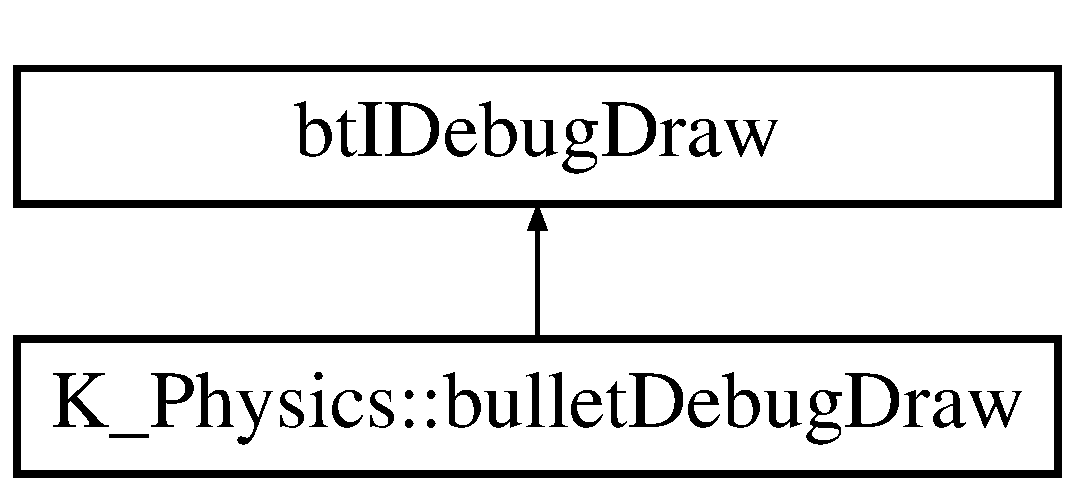
\includegraphics[height=2.000000cm]{class_k___physics_1_1bullet_debug_draw}
\end{center}
\end{figure}
\subsection*{公開メンバ関数}
\begin{DoxyCompactItemize}
\item 
\mbox{\hyperlink{class_k___physics_1_1bullet_debug_draw_ac969f58383a6b62a778bb16eb4026ad6}{bullet\+Debug\+Draw}} ()
\item 
\mbox{\hyperlink{class_k___physics_1_1bullet_debug_draw_a2b26e0588632a32ecef03088f0486378}{$\sim$bullet\+Debug\+Draw}} ()
\item 
void \mbox{\hyperlink{class_k___physics_1_1bullet_debug_draw_a361177ad23a76003b5e0811e4d3643d5}{draw\+Line}} (const bt\+Vector3 \&from, const bt\+Vector3 \&to, const bt\+Vector3 \&color)
\item 
void \mbox{\hyperlink{class_k___physics_1_1bullet_debug_draw_a0842dd424336cc1e332cd2c01f68ac86}{draw\+Line}} (const bt\+Vector3 \&from, const bt\+Vector3 \&to, const bt\+Vector3 \&from\+Color, const bt\+Vector3 \&to\+Color)
\item 
void \mbox{\hyperlink{class_k___physics_1_1bullet_debug_draw_aee36880ac9b46c4379317b8f6d77d312}{draw\+Contact\+Point}} (const bt\+Vector3 \&Point\+OnB, const bt\+Vector3 \&normal\+OnB, bt\+Scalar distance, int life\+Time, const bt\+Vector3 \&color)
\item 
void \mbox{\hyperlink{class_k___physics_1_1bullet_debug_draw_aa421c8d4afa407e1e8c9784fce42115e}{report\+Error\+Warning}} (const char $\ast$warning\+String)
\item 
void \mbox{\hyperlink{class_k___physics_1_1bullet_debug_draw_ad3e665ca605b58a03474ccafc02a5bd9}{draw3d\+Text}} (const bt\+Vector3 \&location, const char $\ast$text\+String)
\item 
void \mbox{\hyperlink{class_k___physics_1_1bullet_debug_draw_a1502ab78aca04f7cae91532fb24a4875}{set\+Debug\+Mode}} (int debug\+Mode)
\item 
int \mbox{\hyperlink{class_k___physics_1_1bullet_debug_draw_aafca54d1beeece0bcaaf3da4765e7699}{get\+Debug\+Mode}} () const
\end{DoxyCompactItemize}


\subsection{構築子と解体子}
\mbox{\Hypertarget{class_k___physics_1_1bullet_debug_draw_ac969f58383a6b62a778bb16eb4026ad6}\label{class_k___physics_1_1bullet_debug_draw_ac969f58383a6b62a778bb16eb4026ad6}} 
\index{K\+\_\+\+Physics\+::bullet\+Debug\+Draw@{K\+\_\+\+Physics\+::bullet\+Debug\+Draw}!bullet\+Debug\+Draw@{bullet\+Debug\+Draw}}
\index{bullet\+Debug\+Draw@{bullet\+Debug\+Draw}!K\+\_\+\+Physics\+::bullet\+Debug\+Draw@{K\+\_\+\+Physics\+::bullet\+Debug\+Draw}}
\subsubsection{\texorpdfstring{bullet\+Debug\+Draw()}{bulletDebugDraw()}}
{\footnotesize\ttfamily K\+\_\+\+Physics\+::bullet\+Debug\+Draw\+::bullet\+Debug\+Draw (\begin{DoxyParamCaption}{ }\end{DoxyParamCaption})}

\mbox{\Hypertarget{class_k___physics_1_1bullet_debug_draw_a2b26e0588632a32ecef03088f0486378}\label{class_k___physics_1_1bullet_debug_draw_a2b26e0588632a32ecef03088f0486378}} 
\index{K\+\_\+\+Physics\+::bullet\+Debug\+Draw@{K\+\_\+\+Physics\+::bullet\+Debug\+Draw}!````~bullet\+Debug\+Draw@{$\sim$bullet\+Debug\+Draw}}
\index{````~bullet\+Debug\+Draw@{$\sim$bullet\+Debug\+Draw}!K\+\_\+\+Physics\+::bullet\+Debug\+Draw@{K\+\_\+\+Physics\+::bullet\+Debug\+Draw}}
\subsubsection{\texorpdfstring{$\sim$bullet\+Debug\+Draw()}{~bulletDebugDraw()}}
{\footnotesize\ttfamily K\+\_\+\+Physics\+::bullet\+Debug\+Draw\+::$\sim$bullet\+Debug\+Draw (\begin{DoxyParamCaption}{ }\end{DoxyParamCaption})}



\subsection{関数詳解}
\mbox{\Hypertarget{class_k___physics_1_1bullet_debug_draw_ad3e665ca605b58a03474ccafc02a5bd9}\label{class_k___physics_1_1bullet_debug_draw_ad3e665ca605b58a03474ccafc02a5bd9}} 
\index{K\+\_\+\+Physics\+::bullet\+Debug\+Draw@{K\+\_\+\+Physics\+::bullet\+Debug\+Draw}!draw3d\+Text@{draw3d\+Text}}
\index{draw3d\+Text@{draw3d\+Text}!K\+\_\+\+Physics\+::bullet\+Debug\+Draw@{K\+\_\+\+Physics\+::bullet\+Debug\+Draw}}
\subsubsection{\texorpdfstring{draw3d\+Text()}{draw3dText()}}
{\footnotesize\ttfamily void K\+\_\+\+Physics\+::bullet\+Debug\+Draw\+::draw3d\+Text (\begin{DoxyParamCaption}\item[{const bt\+Vector3 \&}]{location,  }\item[{const char $\ast$}]{text\+String }\end{DoxyParamCaption})}

\mbox{\Hypertarget{class_k___physics_1_1bullet_debug_draw_aee36880ac9b46c4379317b8f6d77d312}\label{class_k___physics_1_1bullet_debug_draw_aee36880ac9b46c4379317b8f6d77d312}} 
\index{K\+\_\+\+Physics\+::bullet\+Debug\+Draw@{K\+\_\+\+Physics\+::bullet\+Debug\+Draw}!draw\+Contact\+Point@{draw\+Contact\+Point}}
\index{draw\+Contact\+Point@{draw\+Contact\+Point}!K\+\_\+\+Physics\+::bullet\+Debug\+Draw@{K\+\_\+\+Physics\+::bullet\+Debug\+Draw}}
\subsubsection{\texorpdfstring{draw\+Contact\+Point()}{drawContactPoint()}}
{\footnotesize\ttfamily void K\+\_\+\+Physics\+::bullet\+Debug\+Draw\+::draw\+Contact\+Point (\begin{DoxyParamCaption}\item[{const bt\+Vector3 \&}]{Point\+OnB,  }\item[{const bt\+Vector3 \&}]{normal\+OnB,  }\item[{bt\+Scalar}]{distance,  }\item[{int}]{life\+Time,  }\item[{const bt\+Vector3 \&}]{color }\end{DoxyParamCaption})}

\mbox{\Hypertarget{class_k___physics_1_1bullet_debug_draw_a361177ad23a76003b5e0811e4d3643d5}\label{class_k___physics_1_1bullet_debug_draw_a361177ad23a76003b5e0811e4d3643d5}} 
\index{K\+\_\+\+Physics\+::bullet\+Debug\+Draw@{K\+\_\+\+Physics\+::bullet\+Debug\+Draw}!draw\+Line@{draw\+Line}}
\index{draw\+Line@{draw\+Line}!K\+\_\+\+Physics\+::bullet\+Debug\+Draw@{K\+\_\+\+Physics\+::bullet\+Debug\+Draw}}
\subsubsection{\texorpdfstring{draw\+Line()}{drawLine()}\hspace{0.1cm}{\footnotesize\ttfamily [1/2]}}
{\footnotesize\ttfamily void K\+\_\+\+Physics\+::bullet\+Debug\+Draw\+::draw\+Line (\begin{DoxyParamCaption}\item[{const bt\+Vector3 \&}]{from,  }\item[{const bt\+Vector3 \&}]{to,  }\item[{const bt\+Vector3 \&}]{color }\end{DoxyParamCaption})}

\mbox{\Hypertarget{class_k___physics_1_1bullet_debug_draw_a0842dd424336cc1e332cd2c01f68ac86}\label{class_k___physics_1_1bullet_debug_draw_a0842dd424336cc1e332cd2c01f68ac86}} 
\index{K\+\_\+\+Physics\+::bullet\+Debug\+Draw@{K\+\_\+\+Physics\+::bullet\+Debug\+Draw}!draw\+Line@{draw\+Line}}
\index{draw\+Line@{draw\+Line}!K\+\_\+\+Physics\+::bullet\+Debug\+Draw@{K\+\_\+\+Physics\+::bullet\+Debug\+Draw}}
\subsubsection{\texorpdfstring{draw\+Line()}{drawLine()}\hspace{0.1cm}{\footnotesize\ttfamily [2/2]}}
{\footnotesize\ttfamily void K\+\_\+\+Physics\+::bullet\+Debug\+Draw\+::draw\+Line (\begin{DoxyParamCaption}\item[{const bt\+Vector3 \&}]{from,  }\item[{const bt\+Vector3 \&}]{to,  }\item[{const bt\+Vector3 \&}]{from\+Color,  }\item[{const bt\+Vector3 \&}]{to\+Color }\end{DoxyParamCaption})}

\mbox{\Hypertarget{class_k___physics_1_1bullet_debug_draw_aafca54d1beeece0bcaaf3da4765e7699}\label{class_k___physics_1_1bullet_debug_draw_aafca54d1beeece0bcaaf3da4765e7699}} 
\index{K\+\_\+\+Physics\+::bullet\+Debug\+Draw@{K\+\_\+\+Physics\+::bullet\+Debug\+Draw}!get\+Debug\+Mode@{get\+Debug\+Mode}}
\index{get\+Debug\+Mode@{get\+Debug\+Mode}!K\+\_\+\+Physics\+::bullet\+Debug\+Draw@{K\+\_\+\+Physics\+::bullet\+Debug\+Draw}}
\subsubsection{\texorpdfstring{get\+Debug\+Mode()}{getDebugMode()}}
{\footnotesize\ttfamily int K\+\_\+\+Physics\+::bullet\+Debug\+Draw\+::get\+Debug\+Mode (\begin{DoxyParamCaption}{ }\end{DoxyParamCaption}) const}

\mbox{\Hypertarget{class_k___physics_1_1bullet_debug_draw_aa421c8d4afa407e1e8c9784fce42115e}\label{class_k___physics_1_1bullet_debug_draw_aa421c8d4afa407e1e8c9784fce42115e}} 
\index{K\+\_\+\+Physics\+::bullet\+Debug\+Draw@{K\+\_\+\+Physics\+::bullet\+Debug\+Draw}!report\+Error\+Warning@{report\+Error\+Warning}}
\index{report\+Error\+Warning@{report\+Error\+Warning}!K\+\_\+\+Physics\+::bullet\+Debug\+Draw@{K\+\_\+\+Physics\+::bullet\+Debug\+Draw}}
\subsubsection{\texorpdfstring{report\+Error\+Warning()}{reportErrorWarning()}}
{\footnotesize\ttfamily void K\+\_\+\+Physics\+::bullet\+Debug\+Draw\+::report\+Error\+Warning (\begin{DoxyParamCaption}\item[{const char $\ast$}]{warning\+String }\end{DoxyParamCaption})}

\mbox{\Hypertarget{class_k___physics_1_1bullet_debug_draw_a1502ab78aca04f7cae91532fb24a4875}\label{class_k___physics_1_1bullet_debug_draw_a1502ab78aca04f7cae91532fb24a4875}} 
\index{K\+\_\+\+Physics\+::bullet\+Debug\+Draw@{K\+\_\+\+Physics\+::bullet\+Debug\+Draw}!set\+Debug\+Mode@{set\+Debug\+Mode}}
\index{set\+Debug\+Mode@{set\+Debug\+Mode}!K\+\_\+\+Physics\+::bullet\+Debug\+Draw@{K\+\_\+\+Physics\+::bullet\+Debug\+Draw}}
\subsubsection{\texorpdfstring{set\+Debug\+Mode()}{setDebugMode()}}
{\footnotesize\ttfamily void K\+\_\+\+Physics\+::bullet\+Debug\+Draw\+::set\+Debug\+Mode (\begin{DoxyParamCaption}\item[{int}]{debug\+Mode }\end{DoxyParamCaption})}


\hypertarget{class_k___physics_1_1_bullet_physics}{}\section{K\+\_\+\+Physics\+:\+:Bullet\+Physics クラス}
\label{class_k___physics_1_1_bullet_physics}\index{K\+\_\+\+Physics\+::\+Bullet\+Physics@{K\+\_\+\+Physics\+::\+Bullet\+Physics}}


bulletのワールドを管理するクラス~\newline
コリジョンの生成・判定関数を提供している  




{\ttfamily \#include $<$Bullet\+Physics.\+h$>$}

\subsection*{公開メンバ関数}
\begin{DoxyCompactItemize}
\item 
\mbox{\hyperlink{class_k___physics_1_1_bullet_physics_a8c8e7b9c5c8c53861e409aa7a6a644f4}{Bullet\+Physics}} ()
\begin{DoxyCompactList}\small\item\em \mbox{\hyperlink{class_k___physics_1_1_bullet_physics_ad280b1eeb62f13463d47be6182d5b978}{Initialize()}}を呼ぶ \end{DoxyCompactList}\item 
\mbox{\hyperlink{class_k___physics_1_1_bullet_physics_a0fca03e6a99d9cc53cc86f54629f23a7}{$\sim$\+Bullet\+Physics}} ()
\begin{DoxyCompactList}\small\item\em \mbox{\hyperlink{class_k___physics_1_1_bullet_physics_ae7d67b163870213501e3bba697981b35}{Finalize()}}を呼ぶ \end{DoxyCompactList}\item 
bool \mbox{\hyperlink{class_k___physics_1_1_bullet_physics_ad280b1eeb62f13463d47be6182d5b978}{Initialize}} ()
\begin{DoxyCompactList}\small\item\em bulletの初期化を行う \end{DoxyCompactList}\item 
void \mbox{\hyperlink{class_k___physics_1_1_bullet_physics_ae7d67b163870213501e3bba697981b35}{Finalize}} ()
\begin{DoxyCompactList}\small\item\em bulletの終了処理を行う \end{DoxyCompactList}\item 
void \mbox{\hyperlink{class_k___physics_1_1_bullet_physics_a251957471a8ab4f8bbace69c995d325f}{Run}} ()
\begin{DoxyCompactList}\small\item\em bulletの物理世界を更新して座標を変更する~\newline
プレイヤーの地形判定関数は別駆動なのでフレームの初めに呼ぶとよい \end{DoxyCompactList}\item 
void \mbox{\hyperlink{class_k___physics_1_1_bullet_physics_a772c665942f1e1855cd218f50b44a9d7}{Debug\+Draw}} (\mbox{\hyperlink{class_k___graphics_1_1_shader_class}{K\+\_\+\+Graphics\+::\+Shader\+Class}} $\ast$shader, \mbox{\hyperlink{class_k___graphics_1_1_camera_class}{K\+\_\+\+Graphics\+::\+Camera\+Class}} $\ast$camera, const \mbox{\hyperlink{namespace_k___math_a345271af9d32dff2c964bc679b13b45c}{K\+\_\+\+Math\+::\+Matrix4x4}} \&trans=K\+\_\+\+Math\+::\+Matrix4x4\+::\+Identity())
\begin{DoxyCompactList}\small\item\em bulletのコリジョンを可視化する \end{DoxyCompactList}\item 
bt\+Collision\+Shape $\ast$ \mbox{\hyperlink{class_k___physics_1_1_bullet_physics_a70d73ada453638ed643a117b6b2a9809}{Create\+Triangle\+Hull\+Shape}} (const bt\+Vector3 \&point1, const bt\+Vector3 \&point2, const bt\+Vector3 \&point3)
\begin{DoxyCompactList}\small\item\em 三角形の形状を作成 \end{DoxyCompactList}\item 
bt\+Triangle\+Mesh $\ast$ \mbox{\hyperlink{class_k___physics_1_1_bullet_physics_a22e01fd34d8040fb70f4ccf12d69969e}{Create\+Triangle\+Mesh}} (bt\+Vector3 $\ast$vectice, int num\+Face)
\begin{DoxyCompactList}\small\item\em ポリゴンの集合形状を作成 \end{DoxyCompactList}\item 
bt\+Collision\+Shape $\ast$ \mbox{\hyperlink{class_k___physics_1_1_bullet_physics_ad78ad1e12f268bac61731b636ea040b4}{Create\+Triangle\+Mesh\+Shape}} (bt\+Triangle\+Mesh $\ast$mesh)
\begin{DoxyCompactList}\small\item\em bt\+Triangle\+Meshからメッシュ形状を作成 \end{DoxyCompactList}\item 
bt\+Collision\+Shape $\ast$ \mbox{\hyperlink{class_k___physics_1_1_bullet_physics_af6f877441f5b5d7da250bcc39a694273}{Create\+Sphere\+Shape}} (float radius)
\begin{DoxyCompactList}\small\item\em 球の形状を作成 \end{DoxyCompactList}\item 
bt\+Collision\+Shape $\ast$ \mbox{\hyperlink{class_k___physics_1_1_bullet_physics_a67e200395443fdfb27aef63b0e154078}{Create\+Capsule\+Shape}} (float radius, float height)
\begin{DoxyCompactList}\small\item\em カプセルの形状を作成 \end{DoxyCompactList}\item 
bt\+Collision\+Shape $\ast$ \mbox{\hyperlink{class_k___physics_1_1_bullet_physics_a12af3e18b74c5dd8bf6a866f6eb1df03}{Create\+Box\+Shape}} (float half\+Width, float half\+Height, float half\+Depth)
\begin{DoxyCompactList}\small\item\em 直方体の形状を作成 \end{DoxyCompactList}\item 
\mbox{\hyperlink{class_k___physics_1_1_collision_data}{Collision\+Data}} $\ast$ \mbox{\hyperlink{class_k___physics_1_1_bullet_physics_ad8d394a940bd7504521d3345173b15cc}{Create\+Rigid\+Body}} (bt\+Collision\+Shape $\ast$shape, bt\+Scalar mass, int mask, const bt\+Vector3 \&pos=bt\+Vector3(0, 0, 0), const bt\+Vector3 \&rot=bt\+Vector3(0, 0, 0))
\begin{DoxyCompactList}\small\item\em 剛体オブジェクトを作成し、ポインタを返す \end{DoxyCompactList}\item 
\mbox{\hyperlink{class_k___physics_1_1_collision_data}{Collision\+Data}} $\ast$ \mbox{\hyperlink{class_k___physics_1_1_bullet_physics_ae8587763df623623783cce96a444ea15}{Create\+Collision\+Object}} (bt\+Collision\+Shape $\ast$shape, bool ghost, int mask, const bt\+Vector3 \&pos=bt\+Vector3(0, 0, 0), const bt\+Vector3 \&rot=bt\+Vector3(0, 0, 0))
\begin{DoxyCompactList}\small\item\em コリジョンオブジェクトを作成し、ポインタを返す \end{DoxyCompactList}\item 
void \mbox{\hyperlink{class_k___physics_1_1_bullet_physics_ad5e9e30666e87099f84dc5b2c009c4d4}{Remove\+Collision\+Object}} (bt\+Collision\+Object $\ast$rigidbody)
\begin{DoxyCompactList}\small\item\em 明示的に世界に登録している剛体を世界から外してからポインタをdeleteする~\newline
このクラスのデストラクタにてこの関数によって全て開放している \end{DoxyCompactList}\item 
void \mbox{\hyperlink{class_k___physics_1_1_bullet_physics_a1501fdf81207cffa2b1b964d6a38129e}{Remove\+Collision\+Shape}} (bt\+Collision\+Shape $\ast$shape)
\begin{DoxyCompactList}\small\item\em 明示的にリストに存在する形状情報をリストから外してdeleteする この関数を呼ばなくても、このクラスのデストラクタで全て開放している この関数の後は、形状へのポインタは使えないので注意 \end{DoxyCompactList}\item 
void \mbox{\hyperlink{class_k___physics_1_1_bullet_physics_a2064ce3d899413b10a2c77e1294c8e53}{Move\+Character}} (bt\+Collision\+Object $\ast$obj, const bt\+Vector3 \&move)
\begin{DoxyCompactList}\small\item\em 操作性を意識したコリジョンの移動、壁判定も行う(重いが正確) \end{DoxyCompactList}\item 
void \mbox{\hyperlink{class_k___physics_1_1_bullet_physics_af3ed7672b8971271c02610906cab62be}{Move\+Character\+Discrete}} (bt\+Collision\+Object $\ast$obj, const bt\+Vector3 \&h\+Move, const bt\+Vector3 \&v\+Move)
\begin{DoxyCompactList}\small\item\em 離散的なコリジョンの移動、判定が Move\+Character よりも大雑把(ただし軽い) \end{DoxyCompactList}\item 
std\+::vector$<$ \mbox{\hyperlink{struct_k___physics_1_1_collision_tag}{Collision\+Tag}} $>$ \& \mbox{\hyperlink{class_k___physics_1_1_bullet_physics_ade016d6e87e8dfdcc8d559455a161692}{Find\+Confriction\+Objects}} (bt\+Collision\+Object $\ast$myself)
\begin{DoxyCompactList}\small\item\em 現在の物理世界での特定のオブジェクトに対する衝突のチェック \end{DoxyCompactList}\item 
void \mbox{\hyperlink{class_k___physics_1_1_bullet_physics_ac9b3ed073b61a866485f462fa98ec14c}{Set\+Sky\+Vector}} (const bt\+Vector3 \&vector)
\begin{DoxyCompactList}\small\item\em 重力とは反対方向を指す単位ベクトルを設定、キャラクターの移動に利用する \end{DoxyCompactList}\end{DoxyCompactItemize}


\subsection{詳解}
bulletのワールドを管理するクラス~\newline
コリジョンの生成・判定関数を提供している 

\subsection{構築子と解体子}
\mbox{\Hypertarget{class_k___physics_1_1_bullet_physics_a8c8e7b9c5c8c53861e409aa7a6a644f4}\label{class_k___physics_1_1_bullet_physics_a8c8e7b9c5c8c53861e409aa7a6a644f4}} 
\index{K\+\_\+\+Physics\+::\+Bullet\+Physics@{K\+\_\+\+Physics\+::\+Bullet\+Physics}!Bullet\+Physics@{Bullet\+Physics}}
\index{Bullet\+Physics@{Bullet\+Physics}!K\+\_\+\+Physics\+::\+Bullet\+Physics@{K\+\_\+\+Physics\+::\+Bullet\+Physics}}
\subsubsection{\texorpdfstring{Bullet\+Physics()}{BulletPhysics()}}
{\footnotesize\ttfamily K\+\_\+\+Physics\+::\+Bullet\+Physics\+::\+Bullet\+Physics (\begin{DoxyParamCaption}{ }\end{DoxyParamCaption})}



\mbox{\hyperlink{class_k___physics_1_1_bullet_physics_ad280b1eeb62f13463d47be6182d5b978}{Initialize()}}を呼ぶ 

\mbox{\Hypertarget{class_k___physics_1_1_bullet_physics_a0fca03e6a99d9cc53cc86f54629f23a7}\label{class_k___physics_1_1_bullet_physics_a0fca03e6a99d9cc53cc86f54629f23a7}} 
\index{K\+\_\+\+Physics\+::\+Bullet\+Physics@{K\+\_\+\+Physics\+::\+Bullet\+Physics}!````~Bullet\+Physics@{$\sim$\+Bullet\+Physics}}
\index{````~Bullet\+Physics@{$\sim$\+Bullet\+Physics}!K\+\_\+\+Physics\+::\+Bullet\+Physics@{K\+\_\+\+Physics\+::\+Bullet\+Physics}}
\subsubsection{\texorpdfstring{$\sim$\+Bullet\+Physics()}{~BulletPhysics()}}
{\footnotesize\ttfamily K\+\_\+\+Physics\+::\+Bullet\+Physics\+::$\sim$\+Bullet\+Physics (\begin{DoxyParamCaption}{ }\end{DoxyParamCaption})}



\mbox{\hyperlink{class_k___physics_1_1_bullet_physics_ae7d67b163870213501e3bba697981b35}{Finalize()}}を呼ぶ 



\subsection{関数詳解}
\mbox{\Hypertarget{class_k___physics_1_1_bullet_physics_a12af3e18b74c5dd8bf6a866f6eb1df03}\label{class_k___physics_1_1_bullet_physics_a12af3e18b74c5dd8bf6a866f6eb1df03}} 
\index{K\+\_\+\+Physics\+::\+Bullet\+Physics@{K\+\_\+\+Physics\+::\+Bullet\+Physics}!Create\+Box\+Shape@{Create\+Box\+Shape}}
\index{Create\+Box\+Shape@{Create\+Box\+Shape}!K\+\_\+\+Physics\+::\+Bullet\+Physics@{K\+\_\+\+Physics\+::\+Bullet\+Physics}}
\subsubsection{\texorpdfstring{Create\+Box\+Shape()}{CreateBoxShape()}}
{\footnotesize\ttfamily bt\+Collision\+Shape $\ast$ K\+\_\+\+Physics\+::\+Bullet\+Physics\+::\+Create\+Box\+Shape (\begin{DoxyParamCaption}\item[{float}]{half\+Width,  }\item[{float}]{half\+Height,  }\item[{float}]{half\+Depth }\end{DoxyParamCaption})}



直方体の形状を作成 


\begin{DoxyParams}[1]{引数}
\mbox{\tt in}  & {\em half\+Width} & 中心からの直方体の幅 \\
\hline
\mbox{\tt in}  & {\em half\+Height} & 中心からの直方体の高さ \\
\hline
\mbox{\tt in}  & {\em half\+Depth} & 中心からの直方体の奥行き \\
\hline
\end{DoxyParams}
\mbox{\Hypertarget{class_k___physics_1_1_bullet_physics_a67e200395443fdfb27aef63b0e154078}\label{class_k___physics_1_1_bullet_physics_a67e200395443fdfb27aef63b0e154078}} 
\index{K\+\_\+\+Physics\+::\+Bullet\+Physics@{K\+\_\+\+Physics\+::\+Bullet\+Physics}!Create\+Capsule\+Shape@{Create\+Capsule\+Shape}}
\index{Create\+Capsule\+Shape@{Create\+Capsule\+Shape}!K\+\_\+\+Physics\+::\+Bullet\+Physics@{K\+\_\+\+Physics\+::\+Bullet\+Physics}}
\subsubsection{\texorpdfstring{Create\+Capsule\+Shape()}{CreateCapsuleShape()}}
{\footnotesize\ttfamily bt\+Collision\+Shape $\ast$ K\+\_\+\+Physics\+::\+Bullet\+Physics\+::\+Create\+Capsule\+Shape (\begin{DoxyParamCaption}\item[{float}]{radius,  }\item[{float}]{height }\end{DoxyParamCaption})}



カプセルの形状を作成 


\begin{DoxyParams}[1]{引数}
\mbox{\tt in}  & {\em radius} & 球の半径 \\
\hline
\mbox{\tt in}  & {\em height} & カプセルの高さ \\
\hline
\end{DoxyParams}
\mbox{\Hypertarget{class_k___physics_1_1_bullet_physics_ae8587763df623623783cce96a444ea15}\label{class_k___physics_1_1_bullet_physics_ae8587763df623623783cce96a444ea15}} 
\index{K\+\_\+\+Physics\+::\+Bullet\+Physics@{K\+\_\+\+Physics\+::\+Bullet\+Physics}!Create\+Collision\+Object@{Create\+Collision\+Object}}
\index{Create\+Collision\+Object@{Create\+Collision\+Object}!K\+\_\+\+Physics\+::\+Bullet\+Physics@{K\+\_\+\+Physics\+::\+Bullet\+Physics}}
\subsubsection{\texorpdfstring{Create\+Collision\+Object()}{CreateCollisionObject()}}
{\footnotesize\ttfamily \mbox{\hyperlink{class_k___physics_1_1_collision_data}{Collision\+Data}} $\ast$ K\+\_\+\+Physics\+::\+Bullet\+Physics\+::\+Create\+Collision\+Object (\begin{DoxyParamCaption}\item[{bt\+Collision\+Shape $\ast$}]{shape,  }\item[{bool}]{ghost,  }\item[{int}]{mask,  }\item[{const bt\+Vector3 \&}]{pos = {\ttfamily btVector3(0,~0,~0)},  }\item[{const bt\+Vector3 \&}]{rot = {\ttfamily btVector3(0,~0,~0)} }\end{DoxyParamCaption})}



コリジョンオブジェクトを作成し、ポインタを返す 


\begin{DoxyParams}[1]{引数}
\mbox{\tt in}  & {\em shape} & コリジョンの形状へのポインタ \\
\hline
\mbox{\tt in}  & {\em ghost} & コリジョンが剛体と衝突するかのフラグ(trueで剛体とは衝突しない) \\
\hline
\mbox{\tt in}  & {\em mask} & 衝突フィルタに使うビットマスク \\
\hline
\mbox{\tt in}  & {\em pos} & コリジョンの初期位置(省略時はすべて0) \\
\hline
\mbox{\tt in}  & {\em rot} & コリジョンの回転(省略時はすべて0) \\
\hline
\end{DoxyParams}
\mbox{\Hypertarget{class_k___physics_1_1_bullet_physics_ad8d394a940bd7504521d3345173b15cc}\label{class_k___physics_1_1_bullet_physics_ad8d394a940bd7504521d3345173b15cc}} 
\index{K\+\_\+\+Physics\+::\+Bullet\+Physics@{K\+\_\+\+Physics\+::\+Bullet\+Physics}!Create\+Rigid\+Body@{Create\+Rigid\+Body}}
\index{Create\+Rigid\+Body@{Create\+Rigid\+Body}!K\+\_\+\+Physics\+::\+Bullet\+Physics@{K\+\_\+\+Physics\+::\+Bullet\+Physics}}
\subsubsection{\texorpdfstring{Create\+Rigid\+Body()}{CreateRigidBody()}}
{\footnotesize\ttfamily \mbox{\hyperlink{class_k___physics_1_1_collision_data}{Collision\+Data}} $\ast$ K\+\_\+\+Physics\+::\+Bullet\+Physics\+::\+Create\+Rigid\+Body (\begin{DoxyParamCaption}\item[{bt\+Collision\+Shape $\ast$}]{shape,  }\item[{bt\+Scalar}]{mass,  }\item[{int}]{mask,  }\item[{const bt\+Vector3 \&}]{pos = {\ttfamily btVector3(0,~0,~0)},  }\item[{const bt\+Vector3 \&}]{rot = {\ttfamily btVector3(0,~0,~0)} }\end{DoxyParamCaption})}



剛体オブジェクトを作成し、ポインタを返す 


\begin{DoxyParams}[1]{引数}
\mbox{\tt in}  & {\em shape} & 剛体の形状へのポインタ \\
\hline
\mbox{\tt in}  & {\em mass} & 剛体の質量 \\
\hline
\mbox{\tt in}  & {\em mask} & 衝突フィルタに使うビットマスク \\
\hline
\mbox{\tt in}  & {\em pos} & 剛体の初期位置(省略時はすべて0) \\
\hline
\mbox{\tt in}  & {\em rot} & 剛体の回転(省略時はすべて0) \\
\hline
\end{DoxyParams}
\mbox{\Hypertarget{class_k___physics_1_1_bullet_physics_af6f877441f5b5d7da250bcc39a694273}\label{class_k___physics_1_1_bullet_physics_af6f877441f5b5d7da250bcc39a694273}} 
\index{K\+\_\+\+Physics\+::\+Bullet\+Physics@{K\+\_\+\+Physics\+::\+Bullet\+Physics}!Create\+Sphere\+Shape@{Create\+Sphere\+Shape}}
\index{Create\+Sphere\+Shape@{Create\+Sphere\+Shape}!K\+\_\+\+Physics\+::\+Bullet\+Physics@{K\+\_\+\+Physics\+::\+Bullet\+Physics}}
\subsubsection{\texorpdfstring{Create\+Sphere\+Shape()}{CreateSphereShape()}}
{\footnotesize\ttfamily bt\+Collision\+Shape $\ast$ K\+\_\+\+Physics\+::\+Bullet\+Physics\+::\+Create\+Sphere\+Shape (\begin{DoxyParamCaption}\item[{float}]{radius }\end{DoxyParamCaption})}



球の形状を作成 


\begin{DoxyParams}[1]{引数}
\mbox{\tt in}  & {\em radius} & 球の半径 \\
\hline
\end{DoxyParams}
\mbox{\Hypertarget{class_k___physics_1_1_bullet_physics_a70d73ada453638ed643a117b6b2a9809}\label{class_k___physics_1_1_bullet_physics_a70d73ada453638ed643a117b6b2a9809}} 
\index{K\+\_\+\+Physics\+::\+Bullet\+Physics@{K\+\_\+\+Physics\+::\+Bullet\+Physics}!Create\+Triangle\+Hull\+Shape@{Create\+Triangle\+Hull\+Shape}}
\index{Create\+Triangle\+Hull\+Shape@{Create\+Triangle\+Hull\+Shape}!K\+\_\+\+Physics\+::\+Bullet\+Physics@{K\+\_\+\+Physics\+::\+Bullet\+Physics}}
\subsubsection{\texorpdfstring{Create\+Triangle\+Hull\+Shape()}{CreateTriangleHullShape()}}
{\footnotesize\ttfamily bt\+Collision\+Shape $\ast$ K\+\_\+\+Physics\+::\+Bullet\+Physics\+::\+Create\+Triangle\+Hull\+Shape (\begin{DoxyParamCaption}\item[{const bt\+Vector3 \&}]{point1,  }\item[{const bt\+Vector3 \&}]{point2,  }\item[{const bt\+Vector3 \&}]{point3 }\end{DoxyParamCaption})}



三角形の形状を作成 


\begin{DoxyParams}[1]{引数}
\mbox{\tt in}  & {\em point1} & 角の座標 \\
\hline
\mbox{\tt in}  & {\em point2} & 角の座標 \\
\hline
\mbox{\tt in}  & {\em point3} & 角の座標 \\
\hline
\end{DoxyParams}
\mbox{\Hypertarget{class_k___physics_1_1_bullet_physics_a22e01fd34d8040fb70f4ccf12d69969e}\label{class_k___physics_1_1_bullet_physics_a22e01fd34d8040fb70f4ccf12d69969e}} 
\index{K\+\_\+\+Physics\+::\+Bullet\+Physics@{K\+\_\+\+Physics\+::\+Bullet\+Physics}!Create\+Triangle\+Mesh@{Create\+Triangle\+Mesh}}
\index{Create\+Triangle\+Mesh@{Create\+Triangle\+Mesh}!K\+\_\+\+Physics\+::\+Bullet\+Physics@{K\+\_\+\+Physics\+::\+Bullet\+Physics}}
\subsubsection{\texorpdfstring{Create\+Triangle\+Mesh()}{CreateTriangleMesh()}}
{\footnotesize\ttfamily bt\+Triangle\+Mesh $\ast$ K\+\_\+\+Physics\+::\+Bullet\+Physics\+::\+Create\+Triangle\+Mesh (\begin{DoxyParamCaption}\item[{bt\+Vector3 $\ast$}]{vectice,  }\item[{int}]{num\+Face }\end{DoxyParamCaption})}



ポリゴンの集合形状を作成 


\begin{DoxyParams}[1]{引数}
\mbox{\tt in}  & {\em vectice} & 三角形の角座標の配列 \\
\hline
\mbox{\tt in}  & {\em num\+Face} & 三角形の数 \\
\hline
\end{DoxyParams}
\mbox{\Hypertarget{class_k___physics_1_1_bullet_physics_ad78ad1e12f268bac61731b636ea040b4}\label{class_k___physics_1_1_bullet_physics_ad78ad1e12f268bac61731b636ea040b4}} 
\index{K\+\_\+\+Physics\+::\+Bullet\+Physics@{K\+\_\+\+Physics\+::\+Bullet\+Physics}!Create\+Triangle\+Mesh\+Shape@{Create\+Triangle\+Mesh\+Shape}}
\index{Create\+Triangle\+Mesh\+Shape@{Create\+Triangle\+Mesh\+Shape}!K\+\_\+\+Physics\+::\+Bullet\+Physics@{K\+\_\+\+Physics\+::\+Bullet\+Physics}}
\subsubsection{\texorpdfstring{Create\+Triangle\+Mesh\+Shape()}{CreateTriangleMeshShape()}}
{\footnotesize\ttfamily bt\+Collision\+Shape $\ast$ K\+\_\+\+Physics\+::\+Bullet\+Physics\+::\+Create\+Triangle\+Mesh\+Shape (\begin{DoxyParamCaption}\item[{bt\+Triangle\+Mesh $\ast$}]{mesh }\end{DoxyParamCaption})}



bt\+Triangle\+Meshからメッシュ形状を作成 


\begin{DoxyParams}[1]{引数}
\mbox{\tt in}  & {\em mesh} & \mbox{\hyperlink{class_k___physics_1_1_bullet_physics_a22e01fd34d8040fb70f4ccf12d69969e}{Create\+Triangle\+Mesh()}}が返す形状のポインタ \\
\hline
\end{DoxyParams}
\mbox{\Hypertarget{class_k___physics_1_1_bullet_physics_a772c665942f1e1855cd218f50b44a9d7}\label{class_k___physics_1_1_bullet_physics_a772c665942f1e1855cd218f50b44a9d7}} 
\index{K\+\_\+\+Physics\+::\+Bullet\+Physics@{K\+\_\+\+Physics\+::\+Bullet\+Physics}!Debug\+Draw@{Debug\+Draw}}
\index{Debug\+Draw@{Debug\+Draw}!K\+\_\+\+Physics\+::\+Bullet\+Physics@{K\+\_\+\+Physics\+::\+Bullet\+Physics}}
\subsubsection{\texorpdfstring{Debug\+Draw()}{DebugDraw()}}
{\footnotesize\ttfamily void K\+\_\+\+Physics\+::\+Bullet\+Physics\+::\+Debug\+Draw (\begin{DoxyParamCaption}\item[{\mbox{\hyperlink{class_k___graphics_1_1_shader_class}{K\+\_\+\+Graphics\+::\+Shader\+Class}} $\ast$}]{shader,  }\item[{\mbox{\hyperlink{class_k___graphics_1_1_camera_class}{K\+\_\+\+Graphics\+::\+Camera\+Class}} $\ast$}]{camera,  }\item[{const \mbox{\hyperlink{namespace_k___math_a345271af9d32dff2c964bc679b13b45c}{K\+\_\+\+Math\+::\+Matrix4x4}} \&}]{trans = {\ttfamily K\+\_\+Math\+:\+:Matrix4x4\+:\+:Identity()} }\end{DoxyParamCaption})}



bulletのコリジョンを可視化する 


\begin{DoxyParams}[1]{引数}
\mbox{\tt in}  & {\em shader} & 使用するシェーダー \\
\hline
\mbox{\tt in}  & {\em camera} & 使用するカメラ \\
\hline
\mbox{\tt in}  & {\em trans} & 変形行列(省略時単位行列) \\
\hline
\end{DoxyParams}
\mbox{\Hypertarget{class_k___physics_1_1_bullet_physics_ae7d67b163870213501e3bba697981b35}\label{class_k___physics_1_1_bullet_physics_ae7d67b163870213501e3bba697981b35}} 
\index{K\+\_\+\+Physics\+::\+Bullet\+Physics@{K\+\_\+\+Physics\+::\+Bullet\+Physics}!Finalize@{Finalize}}
\index{Finalize@{Finalize}!K\+\_\+\+Physics\+::\+Bullet\+Physics@{K\+\_\+\+Physics\+::\+Bullet\+Physics}}
\subsubsection{\texorpdfstring{Finalize()}{Finalize()}}
{\footnotesize\ttfamily void K\+\_\+\+Physics\+::\+Bullet\+Physics\+::\+Finalize (\begin{DoxyParamCaption}{ }\end{DoxyParamCaption})}



bulletの終了処理を行う 

\mbox{\Hypertarget{class_k___physics_1_1_bullet_physics_ade016d6e87e8dfdcc8d559455a161692}\label{class_k___physics_1_1_bullet_physics_ade016d6e87e8dfdcc8d559455a161692}} 
\index{K\+\_\+\+Physics\+::\+Bullet\+Physics@{K\+\_\+\+Physics\+::\+Bullet\+Physics}!Find\+Confriction\+Objects@{Find\+Confriction\+Objects}}
\index{Find\+Confriction\+Objects@{Find\+Confriction\+Objects}!K\+\_\+\+Physics\+::\+Bullet\+Physics@{K\+\_\+\+Physics\+::\+Bullet\+Physics}}
\subsubsection{\texorpdfstring{Find\+Confriction\+Objects()}{FindConfrictionObjects()}}
{\footnotesize\ttfamily std\+::vector$<$ \mbox{\hyperlink{struct_k___physics_1_1_collision_tag}{Collision\+Tag}} $>$ \& K\+\_\+\+Physics\+::\+Bullet\+Physics\+::\+Find\+Confriction\+Objects (\begin{DoxyParamCaption}\item[{bt\+Collision\+Object $\ast$}]{myself }\end{DoxyParamCaption})}



現在の物理世界での特定のオブジェクトに対する衝突のチェック 


\begin{DoxyParams}[1]{引数}
\mbox{\tt in}  & {\em 衝突をチェックしたいオブジェクト} & \\
\hline
\end{DoxyParams}
\begin{DoxyReturn}{戻り値}
衝突が起こったオブジェクトのタグ情報 
\end{DoxyReturn}
\mbox{\Hypertarget{class_k___physics_1_1_bullet_physics_ad280b1eeb62f13463d47be6182d5b978}\label{class_k___physics_1_1_bullet_physics_ad280b1eeb62f13463d47be6182d5b978}} 
\index{K\+\_\+\+Physics\+::\+Bullet\+Physics@{K\+\_\+\+Physics\+::\+Bullet\+Physics}!Initialize@{Initialize}}
\index{Initialize@{Initialize}!K\+\_\+\+Physics\+::\+Bullet\+Physics@{K\+\_\+\+Physics\+::\+Bullet\+Physics}}
\subsubsection{\texorpdfstring{Initialize()}{Initialize()}}
{\footnotesize\ttfamily bool K\+\_\+\+Physics\+::\+Bullet\+Physics\+::\+Initialize (\begin{DoxyParamCaption}{ }\end{DoxyParamCaption})}



bulletの初期化を行う 

\mbox{\Hypertarget{class_k___physics_1_1_bullet_physics_a2064ce3d899413b10a2c77e1294c8e53}\label{class_k___physics_1_1_bullet_physics_a2064ce3d899413b10a2c77e1294c8e53}} 
\index{K\+\_\+\+Physics\+::\+Bullet\+Physics@{K\+\_\+\+Physics\+::\+Bullet\+Physics}!Move\+Character@{Move\+Character}}
\index{Move\+Character@{Move\+Character}!K\+\_\+\+Physics\+::\+Bullet\+Physics@{K\+\_\+\+Physics\+::\+Bullet\+Physics}}
\subsubsection{\texorpdfstring{Move\+Character()}{MoveCharacter()}}
{\footnotesize\ttfamily void K\+\_\+\+Physics\+::\+Bullet\+Physics\+::\+Move\+Character (\begin{DoxyParamCaption}\item[{bt\+Collision\+Object $\ast$}]{obj,  }\item[{const bt\+Vector3 \&}]{move }\end{DoxyParamCaption})}



操作性を意識したコリジョンの移動、壁判定も行う(重いが正確) 


\begin{DoxyParams}[1]{引数}
\mbox{\tt in}  & {\em obj} & 移動するコリジョンオブジェクト \\
\hline
\mbox{\tt in}  & {\em move} & 移動ベクトル \\
\hline
\end{DoxyParams}
\mbox{\Hypertarget{class_k___physics_1_1_bullet_physics_af3ed7672b8971271c02610906cab62be}\label{class_k___physics_1_1_bullet_physics_af3ed7672b8971271c02610906cab62be}} 
\index{K\+\_\+\+Physics\+::\+Bullet\+Physics@{K\+\_\+\+Physics\+::\+Bullet\+Physics}!Move\+Character\+Discrete@{Move\+Character\+Discrete}}
\index{Move\+Character\+Discrete@{Move\+Character\+Discrete}!K\+\_\+\+Physics\+::\+Bullet\+Physics@{K\+\_\+\+Physics\+::\+Bullet\+Physics}}
\subsubsection{\texorpdfstring{Move\+Character\+Discrete()}{MoveCharacterDiscrete()}}
{\footnotesize\ttfamily void K\+\_\+\+Physics\+::\+Bullet\+Physics\+::\+Move\+Character\+Discrete (\begin{DoxyParamCaption}\item[{bt\+Collision\+Object $\ast$}]{obj,  }\item[{const bt\+Vector3 \&}]{h\+Move,  }\item[{const bt\+Vector3 \&}]{v\+Move }\end{DoxyParamCaption})}



離散的なコリジョンの移動、判定が Move\+Character よりも大雑把(ただし軽い) 


\begin{DoxyParams}[1]{引数}
\mbox{\tt in}  & {\em obj} & 移動するコリジョンオブジェクト \\
\hline
\mbox{\tt in}  & {\em h\+Move} & 横移動ベクトル \\
\hline
\mbox{\tt in}  & {\em v\+Move} & 縦移動ベクトル \\
\hline
\end{DoxyParams}
\mbox{\Hypertarget{class_k___physics_1_1_bullet_physics_ad5e9e30666e87099f84dc5b2c009c4d4}\label{class_k___physics_1_1_bullet_physics_ad5e9e30666e87099f84dc5b2c009c4d4}} 
\index{K\+\_\+\+Physics\+::\+Bullet\+Physics@{K\+\_\+\+Physics\+::\+Bullet\+Physics}!Remove\+Collision\+Object@{Remove\+Collision\+Object}}
\index{Remove\+Collision\+Object@{Remove\+Collision\+Object}!K\+\_\+\+Physics\+::\+Bullet\+Physics@{K\+\_\+\+Physics\+::\+Bullet\+Physics}}
\subsubsection{\texorpdfstring{Remove\+Collision\+Object()}{RemoveCollisionObject()}}
{\footnotesize\ttfamily void K\+\_\+\+Physics\+::\+Bullet\+Physics\+::\+Remove\+Collision\+Object (\begin{DoxyParamCaption}\item[{bt\+Collision\+Object $\ast$}]{rigidbody }\end{DoxyParamCaption})}



明示的に世界に登録している剛体を世界から外してからポインタをdeleteする~\newline
このクラスのデストラクタにてこの関数によって全て開放している 

\mbox{\Hypertarget{class_k___physics_1_1_bullet_physics_a1501fdf81207cffa2b1b964d6a38129e}\label{class_k___physics_1_1_bullet_physics_a1501fdf81207cffa2b1b964d6a38129e}} 
\index{K\+\_\+\+Physics\+::\+Bullet\+Physics@{K\+\_\+\+Physics\+::\+Bullet\+Physics}!Remove\+Collision\+Shape@{Remove\+Collision\+Shape}}
\index{Remove\+Collision\+Shape@{Remove\+Collision\+Shape}!K\+\_\+\+Physics\+::\+Bullet\+Physics@{K\+\_\+\+Physics\+::\+Bullet\+Physics}}
\subsubsection{\texorpdfstring{Remove\+Collision\+Shape()}{RemoveCollisionShape()}}
{\footnotesize\ttfamily void K\+\_\+\+Physics\+::\+Bullet\+Physics\+::\+Remove\+Collision\+Shape (\begin{DoxyParamCaption}\item[{bt\+Collision\+Shape $\ast$}]{shape }\end{DoxyParamCaption})}



明示的にリストに存在する形状情報をリストから外してdeleteする この関数を呼ばなくても、このクラスのデストラクタで全て開放している この関数の後は、形状へのポインタは使えないので注意 

\mbox{\Hypertarget{class_k___physics_1_1_bullet_physics_a251957471a8ab4f8bbace69c995d325f}\label{class_k___physics_1_1_bullet_physics_a251957471a8ab4f8bbace69c995d325f}} 
\index{K\+\_\+\+Physics\+::\+Bullet\+Physics@{K\+\_\+\+Physics\+::\+Bullet\+Physics}!Run@{Run}}
\index{Run@{Run}!K\+\_\+\+Physics\+::\+Bullet\+Physics@{K\+\_\+\+Physics\+::\+Bullet\+Physics}}
\subsubsection{\texorpdfstring{Run()}{Run()}}
{\footnotesize\ttfamily void K\+\_\+\+Physics\+::\+Bullet\+Physics\+::\+Run (\begin{DoxyParamCaption}{ }\end{DoxyParamCaption})}



bulletの物理世界を更新して座標を変更する~\newline
プレイヤーの地形判定関数は別駆動なのでフレームの初めに呼ぶとよい 

\mbox{\Hypertarget{class_k___physics_1_1_bullet_physics_ac9b3ed073b61a866485f462fa98ec14c}\label{class_k___physics_1_1_bullet_physics_ac9b3ed073b61a866485f462fa98ec14c}} 
\index{K\+\_\+\+Physics\+::\+Bullet\+Physics@{K\+\_\+\+Physics\+::\+Bullet\+Physics}!Set\+Sky\+Vector@{Set\+Sky\+Vector}}
\index{Set\+Sky\+Vector@{Set\+Sky\+Vector}!K\+\_\+\+Physics\+::\+Bullet\+Physics@{K\+\_\+\+Physics\+::\+Bullet\+Physics}}
\subsubsection{\texorpdfstring{Set\+Sky\+Vector()}{SetSkyVector()}}
{\footnotesize\ttfamily void K\+\_\+\+Physics\+::\+Bullet\+Physics\+::\+Set\+Sky\+Vector (\begin{DoxyParamCaption}\item[{const bt\+Vector3 \&}]{vector }\end{DoxyParamCaption})}



重力とは反対方向を指す単位ベクトルを設定、キャラクターの移動に利用する 


\begin{DoxyParams}[1]{引数}
\mbox{\tt in}  & {\em vector} & 重力と反対方向の単位ベクトル \\
\hline
\end{DoxyParams}

\hypertarget{struct_k___input_1_1_button_state}{}\section{K\+\_\+\+Input\+:\+:Button\+State 構造体}
\label{struct_k___input_1_1_button_state}\index{K\+\_\+\+Input\+::\+Button\+State@{K\+\_\+\+Input\+::\+Button\+State}}


ジョイパッドの状態  




{\ttfamily \#include $<$Vpad\+States.\+h$>$}

\subsection*{公開変数類}
\begin{DoxyCompactItemize}
\item 
\mbox{\hyperlink{namespace_k___input_a0fad93a64181d6776849d43118c26902}{Joy\+Button}} \mbox{\hyperlink{struct_k___input_1_1_button_state_a7f22bf8e7e2078e45af31f7a1f3a7d2d}{button}}
\item 
\mbox{\hyperlink{namespace_k___input_af62d80c77b12db01035e4b9aa27a09d6}{Key}} \mbox{\hyperlink{struct_k___input_1_1_button_state_a98dffa8b4114f7dfef0750b6444713cb}{keyboard}}
\item 
int \mbox{\hyperlink{struct_k___input_1_1_button_state_a8c2311c266401355c0ff149bd23a2f66}{press}}
\item 
int \mbox{\hyperlink{struct_k___input_1_1_button_state_aec5fd955922f378e854cf9d39877113c}{prev\+Press}}
\end{DoxyCompactItemize}


\subsection{詳解}
ジョイパッドの状態 

\subsection{メンバ詳解}
\mbox{\Hypertarget{struct_k___input_1_1_button_state_a7f22bf8e7e2078e45af31f7a1f3a7d2d}\label{struct_k___input_1_1_button_state_a7f22bf8e7e2078e45af31f7a1f3a7d2d}} 
\index{K\+\_\+\+Input\+::\+Button\+State@{K\+\_\+\+Input\+::\+Button\+State}!button@{button}}
\index{button@{button}!K\+\_\+\+Input\+::\+Button\+State@{K\+\_\+\+Input\+::\+Button\+State}}
\subsubsection{\texorpdfstring{button}{button}}
{\footnotesize\ttfamily \mbox{\hyperlink{namespace_k___input_a0fad93a64181d6776849d43118c26902}{Joy\+Button}} K\+\_\+\+Input\+::\+Button\+State\+::button}

\mbox{\Hypertarget{struct_k___input_1_1_button_state_a98dffa8b4114f7dfef0750b6444713cb}\label{struct_k___input_1_1_button_state_a98dffa8b4114f7dfef0750b6444713cb}} 
\index{K\+\_\+\+Input\+::\+Button\+State@{K\+\_\+\+Input\+::\+Button\+State}!keyboard@{keyboard}}
\index{keyboard@{keyboard}!K\+\_\+\+Input\+::\+Button\+State@{K\+\_\+\+Input\+::\+Button\+State}}
\subsubsection{\texorpdfstring{keyboard}{keyboard}}
{\footnotesize\ttfamily \mbox{\hyperlink{namespace_k___input_af62d80c77b12db01035e4b9aa27a09d6}{Key}} K\+\_\+\+Input\+::\+Button\+State\+::keyboard}

\mbox{\Hypertarget{struct_k___input_1_1_button_state_a8c2311c266401355c0ff149bd23a2f66}\label{struct_k___input_1_1_button_state_a8c2311c266401355c0ff149bd23a2f66}} 
\index{K\+\_\+\+Input\+::\+Button\+State@{K\+\_\+\+Input\+::\+Button\+State}!press@{press}}
\index{press@{press}!K\+\_\+\+Input\+::\+Button\+State@{K\+\_\+\+Input\+::\+Button\+State}}
\subsubsection{\texorpdfstring{press}{press}}
{\footnotesize\ttfamily int K\+\_\+\+Input\+::\+Button\+State\+::press}

\mbox{\Hypertarget{struct_k___input_1_1_button_state_aec5fd955922f378e854cf9d39877113c}\label{struct_k___input_1_1_button_state_aec5fd955922f378e854cf9d39877113c}} 
\index{K\+\_\+\+Input\+::\+Button\+State@{K\+\_\+\+Input\+::\+Button\+State}!prev\+Press@{prev\+Press}}
\index{prev\+Press@{prev\+Press}!K\+\_\+\+Input\+::\+Button\+State@{K\+\_\+\+Input\+::\+Button\+State}}
\subsubsection{\texorpdfstring{prev\+Press}{prevPress}}
{\footnotesize\ttfamily int K\+\_\+\+Input\+::\+Button\+State\+::prev\+Press}


\hypertarget{class_k___graphics_1_1_camera_class}{}\section{K\+\_\+\+Graphics\+:\+:Camera\+Class クラス}
\label{class_k___graphics_1_1_camera_class}\index{K\+\_\+\+Graphics\+::\+Camera\+Class@{K\+\_\+\+Graphics\+::\+Camera\+Class}}


カメラの情報を管理し、ビュー行列と投影行列を提供するクラス  




{\ttfamily \#include $<$Camera\+Class.\+h$>$}

\subsection*{公開メンバ関数}
\begin{DoxyCompactItemize}
\item 
\mbox{\hyperlink{class_k___graphics_1_1_camera_class_a2b371f16a80374ab07522af4bfe8f97c}{Camera\+Class}} (\mbox{\hyperlink{namespace_k___graphics_a46f486e742ad696f88bfbeb22f8af10f}{Camera\+Type}} type, int width, int height, float near, float far, float fov)
\begin{DoxyCompactList}\small\item\em \mbox{\hyperlink{class_k___graphics_1_1_camera_class_af9efd95b7a5b0285c5bda70ca01a002a}{Initialize()}}を呼ぶ \end{DoxyCompactList}\item 
\mbox{\hyperlink{class_k___graphics_1_1_camera_class_a6fadd430bd4da7c246c8e2042c5693af}{$\sim$\+Camera\+Class}} ()
\begin{DoxyCompactList}\small\item\em 特に何もしない \end{DoxyCompactList}\item 
void \mbox{\hyperlink{class_k___graphics_1_1_camera_class_af9efd95b7a5b0285c5bda70ca01a002a}{Initialize}} (\mbox{\hyperlink{namespace_k___graphics_a46f486e742ad696f88bfbeb22f8af10f}{Camera\+Type}} type, int screen\+Width, int screen\+Height, float camera\+Neer, float camera\+Far, float field\+Of\+View)
\begin{DoxyCompactList}\small\item\em カメラを一気に初期化 \end{DoxyCompactList}\item 
void \mbox{\hyperlink{class_k___graphics_1_1_camera_class_a9ca92b03f3171a749da3fabd77743e05}{Draw}} ()
\begin{DoxyCompactList}\small\item\em 行列を作成する、この関数を呼ばない限りカメラは更新されない \end{DoxyCompactList}\item 
const \mbox{\hyperlink{namespace_k___math_a345271af9d32dff2c964bc679b13b45c}{K\+\_\+\+Math\+::\+Matrix4x4}} \& \mbox{\hyperlink{class_k___graphics_1_1_camera_class_a25c8ec2869536e3ba080d5c34749defc}{Get\+View\+Matrix}} ()
\begin{DoxyCompactList}\small\item\em ビュー行列を取得する \end{DoxyCompactList}\item 
const \mbox{\hyperlink{namespace_k___math_a345271af9d32dff2c964bc679b13b45c}{K\+\_\+\+Math\+::\+Matrix4x4}} \& \mbox{\hyperlink{class_k___graphics_1_1_camera_class_a8e972464a146b6f87198debd8571d4e9}{Get\+Camera\+Matrix}} ()
\begin{DoxyCompactList}\small\item\em ビュー行列の逆行列を取得する \end{DoxyCompactList}\item 
const \mbox{\hyperlink{namespace_k___math_a345271af9d32dff2c964bc679b13b45c}{K\+\_\+\+Math\+::\+Matrix4x4}} \& \mbox{\hyperlink{class_k___graphics_1_1_camera_class_a660c15df166e940e7dac70f2dfed98e1}{Get\+Projection\+Matrix}} ()
\begin{DoxyCompactList}\small\item\em 投影行列を取得する \end{DoxyCompactList}\item 
void \mbox{\hyperlink{class_k___graphics_1_1_camera_class_af8264e04ed973e00f3c331d6988f15c1}{Set\+Position}} (float x, float y, float z)
\begin{DoxyCompactList}\small\item\em カメラの座標を指定 \end{DoxyCompactList}\item 
void \mbox{\hyperlink{class_k___graphics_1_1_camera_class_a06189cd5e4c554e46724204053e69a2d}{Set\+Position}} (float distance, const \mbox{\hyperlink{namespace_k___math_a66884d78082c39ada4091c211f3570f8}{K\+\_\+\+Math\+::\+Vector3}} \&vector)
\begin{DoxyCompactList}\small\item\em ターゲットからの方向と距離を指定してカメラ位置を設定 \end{DoxyCompactList}\item 
void \mbox{\hyperlink{class_k___graphics_1_1_camera_class_af40a20fb1f670a489544774c30272188}{Set\+Target}} (float x, float y, float z)
\begin{DoxyCompactList}\small\item\em ターゲット(注視点)を指定 \end{DoxyCompactList}\item 
const \mbox{\hyperlink{namespace_k___math_a66884d78082c39ada4091c211f3570f8}{K\+\_\+\+Math\+::\+Vector3}} \& \mbox{\hyperlink{class_k___graphics_1_1_camera_class_a7ed2ff417ce65d309fb37fdce4805ed1}{Get\+AxisX}} ()
\item 
const \mbox{\hyperlink{namespace_k___math_a66884d78082c39ada4091c211f3570f8}{K\+\_\+\+Math\+::\+Vector3}} \& \mbox{\hyperlink{class_k___graphics_1_1_camera_class_ad66d73d5ab556f074f5d8d082b040f49}{Get\+AxisY}} ()
\item 
const \mbox{\hyperlink{namespace_k___math_a66884d78082c39ada4091c211f3570f8}{K\+\_\+\+Math\+::\+Vector3}} \& \mbox{\hyperlink{class_k___graphics_1_1_camera_class_af7a6866617e0e004b95a6dd33c4396b1}{Get\+AxisZ}} ()
\item 
const \mbox{\hyperlink{namespace_k___math_a66884d78082c39ada4091c211f3570f8}{K\+\_\+\+Math\+::\+Vector3}} \& \mbox{\hyperlink{class_k___graphics_1_1_camera_class_a681845d905fef611bbc88474bc145cdc}{Get\+Terget}} ()
\item 
const \mbox{\hyperlink{namespace_k___math_a66884d78082c39ada4091c211f3570f8}{K\+\_\+\+Math\+::\+Vector3}} \& \mbox{\hyperlink{class_k___graphics_1_1_camera_class_a8ff01ed106d9ee0ac2a6baed8530fa34}{Get\+Position}} ()
\item 
int \mbox{\hyperlink{class_k___graphics_1_1_camera_class_af395ed2ac8596700200324379b38e2f1}{Get\+Screen\+Width}} ()
\item 
int \mbox{\hyperlink{class_k___graphics_1_1_camera_class_a62cca8a08a917056082dacc1f56d05ba}{Get\+Screen\+Height}} ()
\item 
float \mbox{\hyperlink{class_k___graphics_1_1_camera_class_a6d7954b3e2c543b10ccbbca7228f4435}{Get\+Screen\+Near}} ()
\item 
float \mbox{\hyperlink{class_k___graphics_1_1_camera_class_ad7b0263ca8ed5d8b36adda3d9209600d}{Get\+Screen\+Far}} ()
\item 
float \mbox{\hyperlink{class_k___graphics_1_1_camera_class_ae9b70a2f55f2784e14630ae221bcc386}{Get\+Field\+Of\+View}} ()
\begin{DoxyCompactList}\small\item\em 平行投影カメラの場合は値が不定なので注意 \end{DoxyCompactList}\end{DoxyCompactItemize}


\subsection{詳解}
カメラの情報を管理し、ビュー行列と投影行列を提供するクラス 

\subsection{構築子と解体子}
\mbox{\Hypertarget{class_k___graphics_1_1_camera_class_a2b371f16a80374ab07522af4bfe8f97c}\label{class_k___graphics_1_1_camera_class_a2b371f16a80374ab07522af4bfe8f97c}} 
\index{K\+\_\+\+Graphics\+::\+Camera\+Class@{K\+\_\+\+Graphics\+::\+Camera\+Class}!Camera\+Class@{Camera\+Class}}
\index{Camera\+Class@{Camera\+Class}!K\+\_\+\+Graphics\+::\+Camera\+Class@{K\+\_\+\+Graphics\+::\+Camera\+Class}}
\subsubsection{\texorpdfstring{Camera\+Class()}{CameraClass()}}
{\footnotesize\ttfamily K\+\_\+\+Graphics\+::\+Camera\+Class\+::\+Camera\+Class (\begin{DoxyParamCaption}\item[{\mbox{\hyperlink{namespace_k___graphics_a46f486e742ad696f88bfbeb22f8af10f}{Camera\+Type}}}]{type,  }\item[{int}]{width,  }\item[{int}]{height,  }\item[{float}]{near,  }\item[{float}]{far,  }\item[{float}]{fov }\end{DoxyParamCaption})}



\mbox{\hyperlink{class_k___graphics_1_1_camera_class_af9efd95b7a5b0285c5bda70ca01a002a}{Initialize()}}を呼ぶ 

\mbox{\Hypertarget{class_k___graphics_1_1_camera_class_a6fadd430bd4da7c246c8e2042c5693af}\label{class_k___graphics_1_1_camera_class_a6fadd430bd4da7c246c8e2042c5693af}} 
\index{K\+\_\+\+Graphics\+::\+Camera\+Class@{K\+\_\+\+Graphics\+::\+Camera\+Class}!````~Camera\+Class@{$\sim$\+Camera\+Class}}
\index{````~Camera\+Class@{$\sim$\+Camera\+Class}!K\+\_\+\+Graphics\+::\+Camera\+Class@{K\+\_\+\+Graphics\+::\+Camera\+Class}}
\subsubsection{\texorpdfstring{$\sim$\+Camera\+Class()}{~CameraClass()}}
{\footnotesize\ttfamily K\+\_\+\+Graphics\+::\+Camera\+Class\+::$\sim$\+Camera\+Class (\begin{DoxyParamCaption}{ }\end{DoxyParamCaption})}



特に何もしない 



\subsection{関数詳解}
\mbox{\Hypertarget{class_k___graphics_1_1_camera_class_a9ca92b03f3171a749da3fabd77743e05}\label{class_k___graphics_1_1_camera_class_a9ca92b03f3171a749da3fabd77743e05}} 
\index{K\+\_\+\+Graphics\+::\+Camera\+Class@{K\+\_\+\+Graphics\+::\+Camera\+Class}!Draw@{Draw}}
\index{Draw@{Draw}!K\+\_\+\+Graphics\+::\+Camera\+Class@{K\+\_\+\+Graphics\+::\+Camera\+Class}}
\subsubsection{\texorpdfstring{Draw()}{Draw()}}
{\footnotesize\ttfamily void K\+\_\+\+Graphics\+::\+Camera\+Class\+::\+Draw (\begin{DoxyParamCaption}{ }\end{DoxyParamCaption})}



行列を作成する、この関数を呼ばない限りカメラは更新されない 

\mbox{\Hypertarget{class_k___graphics_1_1_camera_class_a7ed2ff417ce65d309fb37fdce4805ed1}\label{class_k___graphics_1_1_camera_class_a7ed2ff417ce65d309fb37fdce4805ed1}} 
\index{K\+\_\+\+Graphics\+::\+Camera\+Class@{K\+\_\+\+Graphics\+::\+Camera\+Class}!Get\+AxisX@{Get\+AxisX}}
\index{Get\+AxisX@{Get\+AxisX}!K\+\_\+\+Graphics\+::\+Camera\+Class@{K\+\_\+\+Graphics\+::\+Camera\+Class}}
\subsubsection{\texorpdfstring{Get\+Axis\+X()}{GetAxisX()}}
{\footnotesize\ttfamily const \mbox{\hyperlink{namespace_k___math_a66884d78082c39ada4091c211f3570f8}{K\+\_\+\+Math\+::\+Vector3}} \& K\+\_\+\+Graphics\+::\+Camera\+Class\+::\+Get\+AxisX (\begin{DoxyParamCaption}{ }\end{DoxyParamCaption})}

\begin{DoxyReturn}{戻り値}
カメラ空間\+X軸の単位ベクトル 
\end{DoxyReturn}
\mbox{\Hypertarget{class_k___graphics_1_1_camera_class_ad66d73d5ab556f074f5d8d082b040f49}\label{class_k___graphics_1_1_camera_class_ad66d73d5ab556f074f5d8d082b040f49}} 
\index{K\+\_\+\+Graphics\+::\+Camera\+Class@{K\+\_\+\+Graphics\+::\+Camera\+Class}!Get\+AxisY@{Get\+AxisY}}
\index{Get\+AxisY@{Get\+AxisY}!K\+\_\+\+Graphics\+::\+Camera\+Class@{K\+\_\+\+Graphics\+::\+Camera\+Class}}
\subsubsection{\texorpdfstring{Get\+Axis\+Y()}{GetAxisY()}}
{\footnotesize\ttfamily const \mbox{\hyperlink{namespace_k___math_a66884d78082c39ada4091c211f3570f8}{K\+\_\+\+Math\+::\+Vector3}} \& K\+\_\+\+Graphics\+::\+Camera\+Class\+::\+Get\+AxisY (\begin{DoxyParamCaption}{ }\end{DoxyParamCaption})}

\begin{DoxyReturn}{戻り値}
カメラ空間\+Y軸の単位ベクトル 
\end{DoxyReturn}
\mbox{\Hypertarget{class_k___graphics_1_1_camera_class_af7a6866617e0e004b95a6dd33c4396b1}\label{class_k___graphics_1_1_camera_class_af7a6866617e0e004b95a6dd33c4396b1}} 
\index{K\+\_\+\+Graphics\+::\+Camera\+Class@{K\+\_\+\+Graphics\+::\+Camera\+Class}!Get\+AxisZ@{Get\+AxisZ}}
\index{Get\+AxisZ@{Get\+AxisZ}!K\+\_\+\+Graphics\+::\+Camera\+Class@{K\+\_\+\+Graphics\+::\+Camera\+Class}}
\subsubsection{\texorpdfstring{Get\+Axis\+Z()}{GetAxisZ()}}
{\footnotesize\ttfamily const \mbox{\hyperlink{namespace_k___math_a66884d78082c39ada4091c211f3570f8}{K\+\_\+\+Math\+::\+Vector3}} \& K\+\_\+\+Graphics\+::\+Camera\+Class\+::\+Get\+AxisZ (\begin{DoxyParamCaption}{ }\end{DoxyParamCaption})}

\begin{DoxyReturn}{戻り値}
カメラ空間\+Z軸の単位ベクトル 
\end{DoxyReturn}
\mbox{\Hypertarget{class_k___graphics_1_1_camera_class_a8e972464a146b6f87198debd8571d4e9}\label{class_k___graphics_1_1_camera_class_a8e972464a146b6f87198debd8571d4e9}} 
\index{K\+\_\+\+Graphics\+::\+Camera\+Class@{K\+\_\+\+Graphics\+::\+Camera\+Class}!Get\+Camera\+Matrix@{Get\+Camera\+Matrix}}
\index{Get\+Camera\+Matrix@{Get\+Camera\+Matrix}!K\+\_\+\+Graphics\+::\+Camera\+Class@{K\+\_\+\+Graphics\+::\+Camera\+Class}}
\subsubsection{\texorpdfstring{Get\+Camera\+Matrix()}{GetCameraMatrix()}}
{\footnotesize\ttfamily const \mbox{\hyperlink{namespace_k___math_a345271af9d32dff2c964bc679b13b45c}{K\+\_\+\+Math\+::\+Matrix4x4}} \& K\+\_\+\+Graphics\+::\+Camera\+Class\+::\+Get\+Camera\+Matrix (\begin{DoxyParamCaption}{ }\end{DoxyParamCaption})}



ビュー行列の逆行列を取得する 

\begin{DoxyReturn}{戻り値}
4x4のビュー変換行列の逆行列 
\end{DoxyReturn}
\mbox{\Hypertarget{class_k___graphics_1_1_camera_class_ae9b70a2f55f2784e14630ae221bcc386}\label{class_k___graphics_1_1_camera_class_ae9b70a2f55f2784e14630ae221bcc386}} 
\index{K\+\_\+\+Graphics\+::\+Camera\+Class@{K\+\_\+\+Graphics\+::\+Camera\+Class}!Get\+Field\+Of\+View@{Get\+Field\+Of\+View}}
\index{Get\+Field\+Of\+View@{Get\+Field\+Of\+View}!K\+\_\+\+Graphics\+::\+Camera\+Class@{K\+\_\+\+Graphics\+::\+Camera\+Class}}
\subsubsection{\texorpdfstring{Get\+Field\+Of\+View()}{GetFieldOfView()}}
{\footnotesize\ttfamily float K\+\_\+\+Graphics\+::\+Camera\+Class\+::\+Get\+Field\+Of\+View (\begin{DoxyParamCaption}{ }\end{DoxyParamCaption})}



平行投影カメラの場合は値が不定なので注意 

\begin{DoxyReturn}{戻り値}
カメラの視野角 
\end{DoxyReturn}
\mbox{\Hypertarget{class_k___graphics_1_1_camera_class_a8ff01ed106d9ee0ac2a6baed8530fa34}\label{class_k___graphics_1_1_camera_class_a8ff01ed106d9ee0ac2a6baed8530fa34}} 
\index{K\+\_\+\+Graphics\+::\+Camera\+Class@{K\+\_\+\+Graphics\+::\+Camera\+Class}!Get\+Position@{Get\+Position}}
\index{Get\+Position@{Get\+Position}!K\+\_\+\+Graphics\+::\+Camera\+Class@{K\+\_\+\+Graphics\+::\+Camera\+Class}}
\subsubsection{\texorpdfstring{Get\+Position()}{GetPosition()}}
{\footnotesize\ttfamily const \mbox{\hyperlink{namespace_k___math_a66884d78082c39ada4091c211f3570f8}{K\+\_\+\+Math\+::\+Vector3}} \& K\+\_\+\+Graphics\+::\+Camera\+Class\+::\+Get\+Position (\begin{DoxyParamCaption}{ }\end{DoxyParamCaption})}

\begin{DoxyReturn}{戻り値}
カメラ位置ベクトル 
\end{DoxyReturn}
\mbox{\Hypertarget{class_k___graphics_1_1_camera_class_a660c15df166e940e7dac70f2dfed98e1}\label{class_k___graphics_1_1_camera_class_a660c15df166e940e7dac70f2dfed98e1}} 
\index{K\+\_\+\+Graphics\+::\+Camera\+Class@{K\+\_\+\+Graphics\+::\+Camera\+Class}!Get\+Projection\+Matrix@{Get\+Projection\+Matrix}}
\index{Get\+Projection\+Matrix@{Get\+Projection\+Matrix}!K\+\_\+\+Graphics\+::\+Camera\+Class@{K\+\_\+\+Graphics\+::\+Camera\+Class}}
\subsubsection{\texorpdfstring{Get\+Projection\+Matrix()}{GetProjectionMatrix()}}
{\footnotesize\ttfamily const \mbox{\hyperlink{namespace_k___math_a345271af9d32dff2c964bc679b13b45c}{K\+\_\+\+Math\+::\+Matrix4x4}} \& K\+\_\+\+Graphics\+::\+Camera\+Class\+::\+Get\+Projection\+Matrix (\begin{DoxyParamCaption}{ }\end{DoxyParamCaption})}



投影行列を取得する 

\begin{DoxyReturn}{戻り値}
4x4の投影変換行列 
\end{DoxyReturn}
\mbox{\Hypertarget{class_k___graphics_1_1_camera_class_ad7b0263ca8ed5d8b36adda3d9209600d}\label{class_k___graphics_1_1_camera_class_ad7b0263ca8ed5d8b36adda3d9209600d}} 
\index{K\+\_\+\+Graphics\+::\+Camera\+Class@{K\+\_\+\+Graphics\+::\+Camera\+Class}!Get\+Screen\+Far@{Get\+Screen\+Far}}
\index{Get\+Screen\+Far@{Get\+Screen\+Far}!K\+\_\+\+Graphics\+::\+Camera\+Class@{K\+\_\+\+Graphics\+::\+Camera\+Class}}
\subsubsection{\texorpdfstring{Get\+Screen\+Far()}{GetScreenFar()}}
{\footnotesize\ttfamily float K\+\_\+\+Graphics\+::\+Camera\+Class\+::\+Get\+Screen\+Far (\begin{DoxyParamCaption}{ }\end{DoxyParamCaption})}

\begin{DoxyReturn}{戻り値}
クリッピング平面の最遠面 
\end{DoxyReturn}
\mbox{\Hypertarget{class_k___graphics_1_1_camera_class_a62cca8a08a917056082dacc1f56d05ba}\label{class_k___graphics_1_1_camera_class_a62cca8a08a917056082dacc1f56d05ba}} 
\index{K\+\_\+\+Graphics\+::\+Camera\+Class@{K\+\_\+\+Graphics\+::\+Camera\+Class}!Get\+Screen\+Height@{Get\+Screen\+Height}}
\index{Get\+Screen\+Height@{Get\+Screen\+Height}!K\+\_\+\+Graphics\+::\+Camera\+Class@{K\+\_\+\+Graphics\+::\+Camera\+Class}}
\subsubsection{\texorpdfstring{Get\+Screen\+Height()}{GetScreenHeight()}}
{\footnotesize\ttfamily int K\+\_\+\+Graphics\+::\+Camera\+Class\+::\+Get\+Screen\+Height (\begin{DoxyParamCaption}{ }\end{DoxyParamCaption})}

\begin{DoxyReturn}{戻り値}
カメラに設定されたビューポート高さ 
\end{DoxyReturn}
\mbox{\Hypertarget{class_k___graphics_1_1_camera_class_a6d7954b3e2c543b10ccbbca7228f4435}\label{class_k___graphics_1_1_camera_class_a6d7954b3e2c543b10ccbbca7228f4435}} 
\index{K\+\_\+\+Graphics\+::\+Camera\+Class@{K\+\_\+\+Graphics\+::\+Camera\+Class}!Get\+Screen\+Near@{Get\+Screen\+Near}}
\index{Get\+Screen\+Near@{Get\+Screen\+Near}!K\+\_\+\+Graphics\+::\+Camera\+Class@{K\+\_\+\+Graphics\+::\+Camera\+Class}}
\subsubsection{\texorpdfstring{Get\+Screen\+Near()}{GetScreenNear()}}
{\footnotesize\ttfamily float K\+\_\+\+Graphics\+::\+Camera\+Class\+::\+Get\+Screen\+Near (\begin{DoxyParamCaption}{ }\end{DoxyParamCaption})}

\begin{DoxyReturn}{戻り値}
クリッピング平面の最近面 
\end{DoxyReturn}
\mbox{\Hypertarget{class_k___graphics_1_1_camera_class_af395ed2ac8596700200324379b38e2f1}\label{class_k___graphics_1_1_camera_class_af395ed2ac8596700200324379b38e2f1}} 
\index{K\+\_\+\+Graphics\+::\+Camera\+Class@{K\+\_\+\+Graphics\+::\+Camera\+Class}!Get\+Screen\+Width@{Get\+Screen\+Width}}
\index{Get\+Screen\+Width@{Get\+Screen\+Width}!K\+\_\+\+Graphics\+::\+Camera\+Class@{K\+\_\+\+Graphics\+::\+Camera\+Class}}
\subsubsection{\texorpdfstring{Get\+Screen\+Width()}{GetScreenWidth()}}
{\footnotesize\ttfamily int K\+\_\+\+Graphics\+::\+Camera\+Class\+::\+Get\+Screen\+Width (\begin{DoxyParamCaption}{ }\end{DoxyParamCaption})}

\begin{DoxyReturn}{戻り値}
カメラに設定されたビューポート幅 
\end{DoxyReturn}
\mbox{\Hypertarget{class_k___graphics_1_1_camera_class_a681845d905fef611bbc88474bc145cdc}\label{class_k___graphics_1_1_camera_class_a681845d905fef611bbc88474bc145cdc}} 
\index{K\+\_\+\+Graphics\+::\+Camera\+Class@{K\+\_\+\+Graphics\+::\+Camera\+Class}!Get\+Terget@{Get\+Terget}}
\index{Get\+Terget@{Get\+Terget}!K\+\_\+\+Graphics\+::\+Camera\+Class@{K\+\_\+\+Graphics\+::\+Camera\+Class}}
\subsubsection{\texorpdfstring{Get\+Terget()}{GetTerget()}}
{\footnotesize\ttfamily const \mbox{\hyperlink{namespace_k___math_a66884d78082c39ada4091c211f3570f8}{K\+\_\+\+Math\+::\+Vector3}} \& K\+\_\+\+Graphics\+::\+Camera\+Class\+::\+Get\+Terget (\begin{DoxyParamCaption}{ }\end{DoxyParamCaption})}

\begin{DoxyReturn}{戻り値}
注視点ベクトル 
\end{DoxyReturn}
\mbox{\Hypertarget{class_k___graphics_1_1_camera_class_a25c8ec2869536e3ba080d5c34749defc}\label{class_k___graphics_1_1_camera_class_a25c8ec2869536e3ba080d5c34749defc}} 
\index{K\+\_\+\+Graphics\+::\+Camera\+Class@{K\+\_\+\+Graphics\+::\+Camera\+Class}!Get\+View\+Matrix@{Get\+View\+Matrix}}
\index{Get\+View\+Matrix@{Get\+View\+Matrix}!K\+\_\+\+Graphics\+::\+Camera\+Class@{K\+\_\+\+Graphics\+::\+Camera\+Class}}
\subsubsection{\texorpdfstring{Get\+View\+Matrix()}{GetViewMatrix()}}
{\footnotesize\ttfamily const \mbox{\hyperlink{namespace_k___math_a345271af9d32dff2c964bc679b13b45c}{K\+\_\+\+Math\+::\+Matrix4x4}} \& K\+\_\+\+Graphics\+::\+Camera\+Class\+::\+Get\+View\+Matrix (\begin{DoxyParamCaption}{ }\end{DoxyParamCaption})}



ビュー行列を取得する 

\begin{DoxyReturn}{戻り値}
4x4のビュー変換行列 
\end{DoxyReturn}
\mbox{\Hypertarget{class_k___graphics_1_1_camera_class_af9efd95b7a5b0285c5bda70ca01a002a}\label{class_k___graphics_1_1_camera_class_af9efd95b7a5b0285c5bda70ca01a002a}} 
\index{K\+\_\+\+Graphics\+::\+Camera\+Class@{K\+\_\+\+Graphics\+::\+Camera\+Class}!Initialize@{Initialize}}
\index{Initialize@{Initialize}!K\+\_\+\+Graphics\+::\+Camera\+Class@{K\+\_\+\+Graphics\+::\+Camera\+Class}}
\subsubsection{\texorpdfstring{Initialize()}{Initialize()}}
{\footnotesize\ttfamily void K\+\_\+\+Graphics\+::\+Camera\+Class\+::\+Initialize (\begin{DoxyParamCaption}\item[{\mbox{\hyperlink{namespace_k___graphics_a46f486e742ad696f88bfbeb22f8af10f}{Camera\+Type}}}]{type,  }\item[{int}]{screen\+Width,  }\item[{int}]{screen\+Height,  }\item[{float}]{camera\+Neer,  }\item[{float}]{camera\+Far,  }\item[{float}]{field\+Of\+View }\end{DoxyParamCaption})}



カメラを一気に初期化 


\begin{DoxyParams}[1]{引数}
\mbox{\tt in}  & {\em type} & カメラのタイプ \\
\hline
\mbox{\tt in}  & {\em screen\+Width} & ビューポートの幅(アスペクト比を出すのに使用する) \\
\hline
\mbox{\tt in}  & {\em screen\+Height} & ビューポートの高さ(アスペクト比を出すのに使用する) \\
\hline
\mbox{\tt in}  & {\em camera\+Neer} & クリッピング平面の最近面 \\
\hline
\mbox{\tt in}  & {\em camera\+Far} & クリッピング平面の最遠面 \\
\hline
\mbox{\tt in}  & {\em field\+Of\+View} & 縦の視野角 \\
\hline
\end{DoxyParams}
\mbox{\Hypertarget{class_k___graphics_1_1_camera_class_af8264e04ed973e00f3c331d6988f15c1}\label{class_k___graphics_1_1_camera_class_af8264e04ed973e00f3c331d6988f15c1}} 
\index{K\+\_\+\+Graphics\+::\+Camera\+Class@{K\+\_\+\+Graphics\+::\+Camera\+Class}!Set\+Position@{Set\+Position}}
\index{Set\+Position@{Set\+Position}!K\+\_\+\+Graphics\+::\+Camera\+Class@{K\+\_\+\+Graphics\+::\+Camera\+Class}}
\subsubsection{\texorpdfstring{Set\+Position()}{SetPosition()}\hspace{0.1cm}{\footnotesize\ttfamily [1/2]}}
{\footnotesize\ttfamily void K\+\_\+\+Graphics\+::\+Camera\+Class\+::\+Set\+Position (\begin{DoxyParamCaption}\item[{float}]{x,  }\item[{float}]{y,  }\item[{float}]{z }\end{DoxyParamCaption})}



カメラの座標を指定 


\begin{DoxyParams}[1]{引数}
\mbox{\tt in}  & {\em x} & x座標 \\
\hline
\mbox{\tt in}  & {\em y} & y座標 \\
\hline
\mbox{\tt in}  & {\em z} & z座標 \\
\hline
\end{DoxyParams}
\mbox{\Hypertarget{class_k___graphics_1_1_camera_class_a06189cd5e4c554e46724204053e69a2d}\label{class_k___graphics_1_1_camera_class_a06189cd5e4c554e46724204053e69a2d}} 
\index{K\+\_\+\+Graphics\+::\+Camera\+Class@{K\+\_\+\+Graphics\+::\+Camera\+Class}!Set\+Position@{Set\+Position}}
\index{Set\+Position@{Set\+Position}!K\+\_\+\+Graphics\+::\+Camera\+Class@{K\+\_\+\+Graphics\+::\+Camera\+Class}}
\subsubsection{\texorpdfstring{Set\+Position()}{SetPosition()}\hspace{0.1cm}{\footnotesize\ttfamily [2/2]}}
{\footnotesize\ttfamily void K\+\_\+\+Graphics\+::\+Camera\+Class\+::\+Set\+Position (\begin{DoxyParamCaption}\item[{float}]{distance,  }\item[{const \mbox{\hyperlink{namespace_k___math_a66884d78082c39ada4091c211f3570f8}{K\+\_\+\+Math\+::\+Vector3}} \&}]{vector }\end{DoxyParamCaption})}



ターゲットからの方向と距離を指定してカメラ位置を設定 


\begin{DoxyParams}[1]{引数}
\mbox{\tt in}  & {\em distance} & ターゲットからの距離 \\
\hline
\mbox{\tt in}  & {\em vector} & ターゲットから離れる向き \\
\hline
\end{DoxyParams}
\mbox{\Hypertarget{class_k___graphics_1_1_camera_class_af40a20fb1f670a489544774c30272188}\label{class_k___graphics_1_1_camera_class_af40a20fb1f670a489544774c30272188}} 
\index{K\+\_\+\+Graphics\+::\+Camera\+Class@{K\+\_\+\+Graphics\+::\+Camera\+Class}!Set\+Target@{Set\+Target}}
\index{Set\+Target@{Set\+Target}!K\+\_\+\+Graphics\+::\+Camera\+Class@{K\+\_\+\+Graphics\+::\+Camera\+Class}}
\subsubsection{\texorpdfstring{Set\+Target()}{SetTarget()}}
{\footnotesize\ttfamily void K\+\_\+\+Graphics\+::\+Camera\+Class\+::\+Set\+Target (\begin{DoxyParamCaption}\item[{float}]{x,  }\item[{float}]{y,  }\item[{float}]{z }\end{DoxyParamCaption})}



ターゲット(注視点)を指定 


\begin{DoxyParams}[1]{引数}
\mbox{\tt in}  & {\em x} & x座標 \\
\hline
\mbox{\tt in}  & {\em y} & y座標 \\
\hline
\mbox{\tt in}  & {\em z} & z座標 \\
\hline
\end{DoxyParams}

\hypertarget{class_k___graphics_1_1_camera_list}{}\section{K\+\_\+\+Graphics\+:\+:Camera\+List クラス}
\label{class_k___graphics_1_1_camera_list}\index{K\+\_\+\+Graphics\+::\+Camera\+List@{K\+\_\+\+Graphics\+::\+Camera\+List}}


カメラに名前を付けて管理するクラス  




{\ttfamily \#include $<$Camera\+List.\+h$>$}

\subsection*{公開メンバ関数}
\begin{DoxyCompactItemize}
\item 
\mbox{\hyperlink{class_k___graphics_1_1_camera_list_a83eea14d2963da7f46309fc06675da86}{Camera\+List}} ()
\begin{DoxyCompactList}\small\item\em \mbox{\hyperlink{class_k___graphics_1_1_camera_list_a933c12ada5504b803d7ad91f38a709fc}{Initialize()}}を呼ぶ \end{DoxyCompactList}\item 
\mbox{\hyperlink{class_k___graphics_1_1_camera_list_a6bd62a622ec57ba1bfd3266213024f4b}{$\sim$\+Camera\+List}} ()
\begin{DoxyCompactList}\small\item\em \mbox{\hyperlink{class_k___graphics_1_1_camera_list_a933c12ada5504b803d7ad91f38a709fc}{Initialize()}}を呼ぶ \end{DoxyCompactList}\item 
void \mbox{\hyperlink{class_k___graphics_1_1_camera_list_a933c12ada5504b803d7ad91f38a709fc}{Initialize}} ()
\begin{DoxyCompactList}\small\item\em リスト内のカメラクラスを全開放している \end{DoxyCompactList}\item 
void \mbox{\hyperlink{class_k___graphics_1_1_camera_list_a2cb2f2ae77ead81009a8e1677617a4a8}{Add\+Perspective\+Camera}} (const std\+::string \&name, const \mbox{\hyperlink{namespace_k___math_a66884d78082c39ada4091c211f3570f8}{K\+\_\+\+Math\+::\+Vector3}} \&position, const \mbox{\hyperlink{namespace_k___math_a66884d78082c39ada4091c211f3570f8}{K\+\_\+\+Math\+::\+Vector3}} \&target, int screen\+Width, int screen\+Height, float camera\+Neer, float camera\+Far, float field\+Of\+View)
\begin{DoxyCompactList}\small\item\em 射影投影のカメラを追加する、射影投影か平行投影かは後で変更できる~\newline
同じ名前は登録できない \end{DoxyCompactList}\item 
void \mbox{\hyperlink{class_k___graphics_1_1_camera_list_ae3e95b8007efa81d1552e05a1b6df63b}{Add\+Ortho\+Camera}} (const std\+::string \&name, const \mbox{\hyperlink{namespace_k___math_a66884d78082c39ada4091c211f3570f8}{K\+\_\+\+Math\+::\+Vector3}} \&position, const \mbox{\hyperlink{namespace_k___math_a66884d78082c39ada4091c211f3570f8}{K\+\_\+\+Math\+::\+Vector3}} \&target, int screen\+Width, int screen\+Height, float camera\+Neer, float camera\+Far)
\begin{DoxyCompactList}\small\item\em 平行投影のカメラを追加する、射影投影か平行投影かは後で変更できる~\newline
同じ名前は登録できない \end{DoxyCompactList}\item 
\mbox{\hyperlink{class_k___graphics_1_1_camera_class}{Camera\+Class}} $\ast$ \mbox{\hyperlink{class_k___graphics_1_1_camera_list_aa4f8101671c5d4c548853891738b6265}{Get\+Camera}} (const std\+::string \&name)
\begin{DoxyCompactList}\small\item\em 名前からカメラを取得する \end{DoxyCompactList}\end{DoxyCompactItemize}


\subsection{詳解}
カメラに名前を付けて管理するクラス 

\subsection{構築子と解体子}
\mbox{\Hypertarget{class_k___graphics_1_1_camera_list_a83eea14d2963da7f46309fc06675da86}\label{class_k___graphics_1_1_camera_list_a83eea14d2963da7f46309fc06675da86}} 
\index{K\+\_\+\+Graphics\+::\+Camera\+List@{K\+\_\+\+Graphics\+::\+Camera\+List}!Camera\+List@{Camera\+List}}
\index{Camera\+List@{Camera\+List}!K\+\_\+\+Graphics\+::\+Camera\+List@{K\+\_\+\+Graphics\+::\+Camera\+List}}
\subsubsection{\texorpdfstring{Camera\+List()}{CameraList()}}
{\footnotesize\ttfamily K\+\_\+\+Graphics\+::\+Camera\+List\+::\+Camera\+List (\begin{DoxyParamCaption}{ }\end{DoxyParamCaption})}



\mbox{\hyperlink{class_k___graphics_1_1_camera_list_a933c12ada5504b803d7ad91f38a709fc}{Initialize()}}を呼ぶ 

\mbox{\Hypertarget{class_k___graphics_1_1_camera_list_a6bd62a622ec57ba1bfd3266213024f4b}\label{class_k___graphics_1_1_camera_list_a6bd62a622ec57ba1bfd3266213024f4b}} 
\index{K\+\_\+\+Graphics\+::\+Camera\+List@{K\+\_\+\+Graphics\+::\+Camera\+List}!````~Camera\+List@{$\sim$\+Camera\+List}}
\index{````~Camera\+List@{$\sim$\+Camera\+List}!K\+\_\+\+Graphics\+::\+Camera\+List@{K\+\_\+\+Graphics\+::\+Camera\+List}}
\subsubsection{\texorpdfstring{$\sim$\+Camera\+List()}{~CameraList()}}
{\footnotesize\ttfamily K\+\_\+\+Graphics\+::\+Camera\+List\+::$\sim$\+Camera\+List (\begin{DoxyParamCaption}{ }\end{DoxyParamCaption})}



\mbox{\hyperlink{class_k___graphics_1_1_camera_list_a933c12ada5504b803d7ad91f38a709fc}{Initialize()}}を呼ぶ 



\subsection{関数詳解}
\mbox{\Hypertarget{class_k___graphics_1_1_camera_list_ae3e95b8007efa81d1552e05a1b6df63b}\label{class_k___graphics_1_1_camera_list_ae3e95b8007efa81d1552e05a1b6df63b}} 
\index{K\+\_\+\+Graphics\+::\+Camera\+List@{K\+\_\+\+Graphics\+::\+Camera\+List}!Add\+Ortho\+Camera@{Add\+Ortho\+Camera}}
\index{Add\+Ortho\+Camera@{Add\+Ortho\+Camera}!K\+\_\+\+Graphics\+::\+Camera\+List@{K\+\_\+\+Graphics\+::\+Camera\+List}}
\subsubsection{\texorpdfstring{Add\+Ortho\+Camera()}{AddOrthoCamera()}}
{\footnotesize\ttfamily void K\+\_\+\+Graphics\+::\+Camera\+List\+::\+Add\+Ortho\+Camera (\begin{DoxyParamCaption}\item[{const std\+::string \&}]{name,  }\item[{const \mbox{\hyperlink{namespace_k___math_a66884d78082c39ada4091c211f3570f8}{K\+\_\+\+Math\+::\+Vector3}} \&}]{position,  }\item[{const \mbox{\hyperlink{namespace_k___math_a66884d78082c39ada4091c211f3570f8}{K\+\_\+\+Math\+::\+Vector3}} \&}]{target,  }\item[{int}]{screen\+Width,  }\item[{int}]{screen\+Height,  }\item[{float}]{camera\+Neer,  }\item[{float}]{camera\+Far }\end{DoxyParamCaption})}



平行投影のカメラを追加する、射影投影か平行投影かは後で変更できる~\newline
同じ名前は登録できない 


\begin{DoxyParams}[1]{引数}
\mbox{\tt in}  & {\em name} & 登録するカメラのユーザー定義名 \\
\hline
\mbox{\tt in}  & {\em position} & カメラ位置 \\
\hline
\mbox{\tt in}  & {\em target} & 注視点位置 \\
\hline
\mbox{\tt in}  & {\em screen\+Width} & ビューポートの幅(アスペクト比を出すのに使用する) \\
\hline
\mbox{\tt in}  & {\em screen\+Height} & ビューポートの高さ(アスペクト比を出すのに使用する) \\
\hline
\mbox{\tt in}  & {\em camera\+Neer} & クリッピング平面の最近面 \\
\hline
\mbox{\tt in}  & {\em camera\+Far} & クリッピング平面の最遠面 \\
\hline
\end{DoxyParams}
\mbox{\Hypertarget{class_k___graphics_1_1_camera_list_a2cb2f2ae77ead81009a8e1677617a4a8}\label{class_k___graphics_1_1_camera_list_a2cb2f2ae77ead81009a8e1677617a4a8}} 
\index{K\+\_\+\+Graphics\+::\+Camera\+List@{K\+\_\+\+Graphics\+::\+Camera\+List}!Add\+Perspective\+Camera@{Add\+Perspective\+Camera}}
\index{Add\+Perspective\+Camera@{Add\+Perspective\+Camera}!K\+\_\+\+Graphics\+::\+Camera\+List@{K\+\_\+\+Graphics\+::\+Camera\+List}}
\subsubsection{\texorpdfstring{Add\+Perspective\+Camera()}{AddPerspectiveCamera()}}
{\footnotesize\ttfamily void K\+\_\+\+Graphics\+::\+Camera\+List\+::\+Add\+Perspective\+Camera (\begin{DoxyParamCaption}\item[{const std\+::string \&}]{name,  }\item[{const \mbox{\hyperlink{namespace_k___math_a66884d78082c39ada4091c211f3570f8}{K\+\_\+\+Math\+::\+Vector3}} \&}]{position,  }\item[{const \mbox{\hyperlink{namespace_k___math_a66884d78082c39ada4091c211f3570f8}{K\+\_\+\+Math\+::\+Vector3}} \&}]{target,  }\item[{int}]{screen\+Width,  }\item[{int}]{screen\+Height,  }\item[{float}]{camera\+Neer,  }\item[{float}]{camera\+Far,  }\item[{float}]{field\+Of\+View }\end{DoxyParamCaption})}



射影投影のカメラを追加する、射影投影か平行投影かは後で変更できる~\newline
同じ名前は登録できない 


\begin{DoxyParams}[1]{引数}
\mbox{\tt in}  & {\em name} & 登録するカメラのユーザー定義名 \\
\hline
\mbox{\tt in}  & {\em position} & カメラ位置 \\
\hline
\mbox{\tt in}  & {\em target} & 注視点位置 \\
\hline
\mbox{\tt in}  & {\em screen\+Width} & ビューポートの幅(アスペクト比を出すのに使用する) \\
\hline
\mbox{\tt in}  & {\em screen\+Height} & ビューポートの高さ(アスペクト比を出すのに使用する) \\
\hline
\mbox{\tt in}  & {\em camera\+Neer} & クリッピング平面の最近面 \\
\hline
\mbox{\tt in}  & {\em camera\+Far} & クリッピング平面の最遠面 \\
\hline
\mbox{\tt in}  & {\em field\+Of\+View} & 縦の視野角 \\
\hline
\end{DoxyParams}
\mbox{\Hypertarget{class_k___graphics_1_1_camera_list_aa4f8101671c5d4c548853891738b6265}\label{class_k___graphics_1_1_camera_list_aa4f8101671c5d4c548853891738b6265}} 
\index{K\+\_\+\+Graphics\+::\+Camera\+List@{K\+\_\+\+Graphics\+::\+Camera\+List}!Get\+Camera@{Get\+Camera}}
\index{Get\+Camera@{Get\+Camera}!K\+\_\+\+Graphics\+::\+Camera\+List@{K\+\_\+\+Graphics\+::\+Camera\+List}}
\subsubsection{\texorpdfstring{Get\+Camera()}{GetCamera()}}
{\footnotesize\ttfamily \mbox{\hyperlink{class_k___graphics_1_1_camera_class}{Camera\+Class}} $\ast$ K\+\_\+\+Graphics\+::\+Camera\+List\+::\+Get\+Camera (\begin{DoxyParamCaption}\item[{const std\+::string \&}]{name }\end{DoxyParamCaption})}



名前からカメラを取得する 


\begin{DoxyParams}[1]{引数}
\mbox{\tt in}  & {\em name} & カメラのユーザー定義名 \\
\hline
\end{DoxyParams}
\begin{DoxyReturn}{戻り値}
その名前のカメラへのポインタ、失敗した場合はnullptr 
\end{DoxyReturn}
\mbox{\Hypertarget{class_k___graphics_1_1_camera_list_a933c12ada5504b803d7ad91f38a709fc}\label{class_k___graphics_1_1_camera_list_a933c12ada5504b803d7ad91f38a709fc}} 
\index{K\+\_\+\+Graphics\+::\+Camera\+List@{K\+\_\+\+Graphics\+::\+Camera\+List}!Initialize@{Initialize}}
\index{Initialize@{Initialize}!K\+\_\+\+Graphics\+::\+Camera\+List@{K\+\_\+\+Graphics\+::\+Camera\+List}}
\subsubsection{\texorpdfstring{Initialize()}{Initialize()}}
{\footnotesize\ttfamily void K\+\_\+\+Graphics\+::\+Camera\+List\+::\+Initialize (\begin{DoxyParamCaption}{ }\end{DoxyParamCaption})}



リスト内のカメラクラスを全開放している 


\hypertarget{struct_k___graphics_1_1_font_generator_1_1_char_data}{}\section{K\+\_\+\+Graphics\+:\+:Font\+Generator\+:\+:Char\+Data 構造体}
\label{struct_k___graphics_1_1_font_generator_1_1_char_data}\index{K\+\_\+\+Graphics\+::\+Font\+Generator\+::\+Char\+Data@{K\+\_\+\+Graphics\+::\+Font\+Generator\+::\+Char\+Data}}


{\ttfamily \#include $<$Font\+Generator.\+h$>$}

\subsection*{公開変数類}
\begin{DoxyCompactItemize}
\item 
std\+::unordered\+\_\+map$<$ int, \mbox{\hyperlink{struct_k___graphics_1_1_font_generator_1_1_font_data}{Font\+Data}} $>$ \mbox{\hyperlink{struct_k___graphics_1_1_font_generator_1_1_char_data_aa0c328dbd5a5188198eecb505ca3bed8}{font\+Data}}
\end{DoxyCompactItemize}


\subsection{メンバ詳解}
\mbox{\Hypertarget{struct_k___graphics_1_1_font_generator_1_1_char_data_aa0c328dbd5a5188198eecb505ca3bed8}\label{struct_k___graphics_1_1_font_generator_1_1_char_data_aa0c328dbd5a5188198eecb505ca3bed8}} 
\index{K\+\_\+\+Graphics\+::\+Font\+Generator\+::\+Char\+Data@{K\+\_\+\+Graphics\+::\+Font\+Generator\+::\+Char\+Data}!font\+Data@{font\+Data}}
\index{font\+Data@{font\+Data}!K\+\_\+\+Graphics\+::\+Font\+Generator\+::\+Char\+Data@{K\+\_\+\+Graphics\+::\+Font\+Generator\+::\+Char\+Data}}
\subsubsection{\texorpdfstring{font\+Data}{fontData}}
{\footnotesize\ttfamily std\+::unordered\+\_\+map$<$int, \mbox{\hyperlink{struct_k___graphics_1_1_font_generator_1_1_font_data}{Font\+Data}}$>$ K\+\_\+\+Graphics\+::\+Font\+Generator\+::\+Char\+Data\+::font\+Data}


\hypertarget{struct_k___physics_1_1_collect_collision_call_back}{}\section{K\+\_\+\+Physics\+:\+:Collect\+Collision\+Call\+Back 構造体}
\label{struct_k___physics_1_1_collect_collision_call_back}\index{K\+\_\+\+Physics\+::\+Collect\+Collision\+Call\+Back@{K\+\_\+\+Physics\+::\+Collect\+Collision\+Call\+Back}}


{\ttfamily \#include $<$Bullet\+Physics.\+h$>$}

K\+\_\+\+Physics\+:\+:Collect\+Collision\+Call\+Back の継承関係図\begin{figure}[H]
\begin{center}
\leavevmode
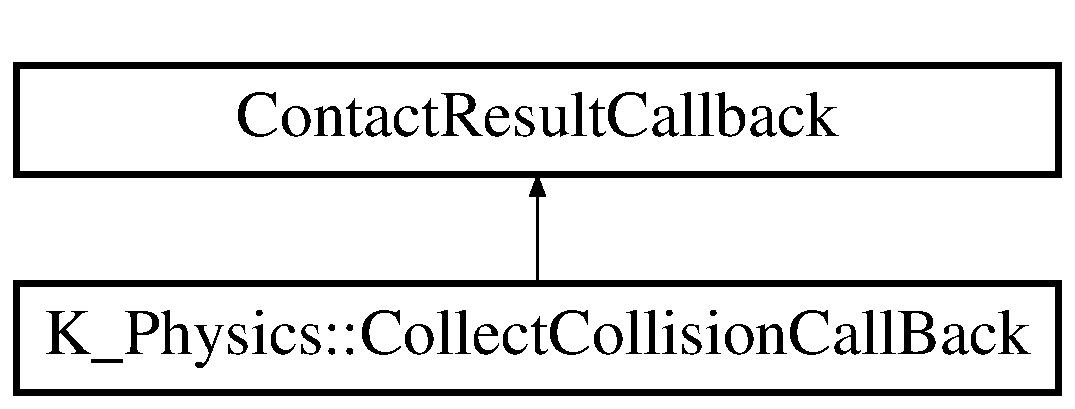
\includegraphics[height=2.000000cm]{struct_k___physics_1_1_collect_collision_call_back}
\end{center}
\end{figure}
\subsection*{公開メンバ関数}
\begin{DoxyCompactItemize}
\item 
\mbox{\hyperlink{struct_k___physics_1_1_collect_collision_call_back_af31aa674f34cfe4dcf0e50a4ac7e0a28}{Collect\+Collision\+Call\+Back}} (std\+::vector$<$ \mbox{\hyperlink{struct_k___physics_1_1_collision_tag}{Collision\+Tag}} $>$ \&tag\+List)
\item 
virtual bt\+Scalar \mbox{\hyperlink{struct_k___physics_1_1_collect_collision_call_back_aab1f994d72f55d819b7cf0a1a371d0ac}{add\+Single\+Result}} (bt\+Manifold\+Point \&cp, const bt\+Collision\+Object\+Wrapper $\ast$col\+Obj0\+Wrap, int part\+Id0, int index0, const bt\+Collision\+Object\+Wrapper $\ast$col\+Obj1\+Wrap, int part\+Id1, int index1)
\end{DoxyCompactItemize}
\subsection*{公開変数類}
\begin{DoxyCompactItemize}
\item 
bt\+Collision\+Object $\ast$ \mbox{\hyperlink{struct_k___physics_1_1_collect_collision_call_back_ac95b38d8abfd6f8cf868ac42878d4dba}{obj}}
\item 
std\+::vector$<$ \mbox{\hyperlink{struct_k___physics_1_1_collision_tag}{Collision\+Tag}} $>$ \& \mbox{\hyperlink{struct_k___physics_1_1_collect_collision_call_back_aa0b6872894b53f34f5c69d14eb23aada}{result}}
\item 
bool \mbox{\hyperlink{struct_k___physics_1_1_collect_collision_call_back_a22aa53d54265d3f318754626ba06031a}{is\+Hit}}
\end{DoxyCompactItemize}


\subsection{構築子と解体子}
\mbox{\Hypertarget{struct_k___physics_1_1_collect_collision_call_back_af31aa674f34cfe4dcf0e50a4ac7e0a28}\label{struct_k___physics_1_1_collect_collision_call_back_af31aa674f34cfe4dcf0e50a4ac7e0a28}} 
\index{K\+\_\+\+Physics\+::\+Collect\+Collision\+Call\+Back@{K\+\_\+\+Physics\+::\+Collect\+Collision\+Call\+Back}!Collect\+Collision\+Call\+Back@{Collect\+Collision\+Call\+Back}}
\index{Collect\+Collision\+Call\+Back@{Collect\+Collision\+Call\+Back}!K\+\_\+\+Physics\+::\+Collect\+Collision\+Call\+Back@{K\+\_\+\+Physics\+::\+Collect\+Collision\+Call\+Back}}
\subsubsection{\texorpdfstring{Collect\+Collision\+Call\+Back()}{CollectCollisionCallBack()}}
{\footnotesize\ttfamily K\+\_\+\+Physics\+::\+Collect\+Collision\+Call\+Back\+::\+Collect\+Collision\+Call\+Back (\begin{DoxyParamCaption}\item[{std\+::vector$<$ \mbox{\hyperlink{struct_k___physics_1_1_collision_tag}{Collision\+Tag}} $>$ \&}]{tag\+List }\end{DoxyParamCaption})}



\subsection{関数詳解}
\mbox{\Hypertarget{struct_k___physics_1_1_collect_collision_call_back_aab1f994d72f55d819b7cf0a1a371d0ac}\label{struct_k___physics_1_1_collect_collision_call_back_aab1f994d72f55d819b7cf0a1a371d0ac}} 
\index{K\+\_\+\+Physics\+::\+Collect\+Collision\+Call\+Back@{K\+\_\+\+Physics\+::\+Collect\+Collision\+Call\+Back}!add\+Single\+Result@{add\+Single\+Result}}
\index{add\+Single\+Result@{add\+Single\+Result}!K\+\_\+\+Physics\+::\+Collect\+Collision\+Call\+Back@{K\+\_\+\+Physics\+::\+Collect\+Collision\+Call\+Back}}
\subsubsection{\texorpdfstring{add\+Single\+Result()}{addSingleResult()}}
{\footnotesize\ttfamily bt\+Scalar K\+\_\+\+Physics\+::\+Collect\+Collision\+Call\+Back\+::add\+Single\+Result (\begin{DoxyParamCaption}\item[{bt\+Manifold\+Point \&}]{cp,  }\item[{const bt\+Collision\+Object\+Wrapper $\ast$}]{col\+Obj0\+Wrap,  }\item[{int}]{part\+Id0,  }\item[{int}]{index0,  }\item[{const bt\+Collision\+Object\+Wrapper $\ast$}]{col\+Obj1\+Wrap,  }\item[{int}]{part\+Id1,  }\item[{int}]{index1 }\end{DoxyParamCaption})\hspace{0.3cm}{\ttfamily [virtual]}}



\subsection{メンバ詳解}
\mbox{\Hypertarget{struct_k___physics_1_1_collect_collision_call_back_a22aa53d54265d3f318754626ba06031a}\label{struct_k___physics_1_1_collect_collision_call_back_a22aa53d54265d3f318754626ba06031a}} 
\index{K\+\_\+\+Physics\+::\+Collect\+Collision\+Call\+Back@{K\+\_\+\+Physics\+::\+Collect\+Collision\+Call\+Back}!is\+Hit@{is\+Hit}}
\index{is\+Hit@{is\+Hit}!K\+\_\+\+Physics\+::\+Collect\+Collision\+Call\+Back@{K\+\_\+\+Physics\+::\+Collect\+Collision\+Call\+Back}}
\subsubsection{\texorpdfstring{is\+Hit}{isHit}}
{\footnotesize\ttfamily bool K\+\_\+\+Physics\+::\+Collect\+Collision\+Call\+Back\+::is\+Hit}

\mbox{\Hypertarget{struct_k___physics_1_1_collect_collision_call_back_ac95b38d8abfd6f8cf868ac42878d4dba}\label{struct_k___physics_1_1_collect_collision_call_back_ac95b38d8abfd6f8cf868ac42878d4dba}} 
\index{K\+\_\+\+Physics\+::\+Collect\+Collision\+Call\+Back@{K\+\_\+\+Physics\+::\+Collect\+Collision\+Call\+Back}!obj@{obj}}
\index{obj@{obj}!K\+\_\+\+Physics\+::\+Collect\+Collision\+Call\+Back@{K\+\_\+\+Physics\+::\+Collect\+Collision\+Call\+Back}}
\subsubsection{\texorpdfstring{obj}{obj}}
{\footnotesize\ttfamily bt\+Collision\+Object$\ast$ K\+\_\+\+Physics\+::\+Collect\+Collision\+Call\+Back\+::obj}

\mbox{\Hypertarget{struct_k___physics_1_1_collect_collision_call_back_aa0b6872894b53f34f5c69d14eb23aada}\label{struct_k___physics_1_1_collect_collision_call_back_aa0b6872894b53f34f5c69d14eb23aada}} 
\index{K\+\_\+\+Physics\+::\+Collect\+Collision\+Call\+Back@{K\+\_\+\+Physics\+::\+Collect\+Collision\+Call\+Back}!result@{result}}
\index{result@{result}!K\+\_\+\+Physics\+::\+Collect\+Collision\+Call\+Back@{K\+\_\+\+Physics\+::\+Collect\+Collision\+Call\+Back}}
\subsubsection{\texorpdfstring{result}{result}}
{\footnotesize\ttfamily std\+::vector$<$\mbox{\hyperlink{struct_k___physics_1_1_collision_tag}{Collision\+Tag}}$>$\& K\+\_\+\+Physics\+::\+Collect\+Collision\+Call\+Back\+::result}


\hypertarget{class_k___physics_1_1_collision_data}{}\section{K\+\_\+\+Physics\+:\+:Collision\+Data クラス}
\label{class_k___physics_1_1_collision_data}\index{K\+\_\+\+Physics\+::\+Collision\+Data@{K\+\_\+\+Physics\+::\+Collision\+Data}}


コリジョンの移動機能を持つ、要はbulletのコリジョン情報を扱いやすくしたクラス  




{\ttfamily \#include $<$Bullet\+Physics.\+h$>$}

\subsection*{公開メンバ関数}
\begin{DoxyCompactItemize}
\item 
\mbox{\hyperlink{class_k___physics_1_1_collision_data_abc664918f597d9ef7ccc00530d6f9c5c}{Collision\+Data}} (bt\+Collision\+Object $\ast$obj, \mbox{\hyperlink{struct_k___physics_1_1_collision_tag}{Collision\+Tag}} \mbox{\hyperlink{class_k___physics_1_1_collision_data_aca2f02c2b5deed664630c0a04c4f2b1f}{tag}})
\item 
void \mbox{\hyperlink{class_k___physics_1_1_collision_data_ae62b85485120979ffbc0be94b371ed5a}{Set\+Collision\+Position}} (const bt\+Vector3 \&position)
\item 
bt\+Vector3 \mbox{\hyperlink{class_k___physics_1_1_collision_data_a2f9a7ee59434120e3d18f66af035db7b}{Get\+Collision\+Position}} ()
\end{DoxyCompactItemize}
\subsection*{公開変数類}
\begin{DoxyCompactItemize}
\item 
bt\+Collision\+Object $\ast$const \mbox{\hyperlink{class_k___physics_1_1_collision_data_a45dc4d1f2a85cef93993b2872c49fc49}{collision}}
\item 
\mbox{\hyperlink{struct_k___physics_1_1_collision_tag}{Collision\+Tag}} \mbox{\hyperlink{class_k___physics_1_1_collision_data_aca2f02c2b5deed664630c0a04c4f2b1f}{tag}}
\end{DoxyCompactItemize}


\subsection{詳解}
コリジョンの移動機能を持つ、要はbulletのコリジョン情報を扱いやすくしたクラス 

\subsection{構築子と解体子}
\mbox{\Hypertarget{class_k___physics_1_1_collision_data_abc664918f597d9ef7ccc00530d6f9c5c}\label{class_k___physics_1_1_collision_data_abc664918f597d9ef7ccc00530d6f9c5c}} 
\index{K\+\_\+\+Physics\+::\+Collision\+Data@{K\+\_\+\+Physics\+::\+Collision\+Data}!Collision\+Data@{Collision\+Data}}
\index{Collision\+Data@{Collision\+Data}!K\+\_\+\+Physics\+::\+Collision\+Data@{K\+\_\+\+Physics\+::\+Collision\+Data}}
\subsubsection{\texorpdfstring{Collision\+Data()}{CollisionData()}}
{\footnotesize\ttfamily K\+\_\+\+Physics\+::\+Collision\+Data\+::\+Collision\+Data (\begin{DoxyParamCaption}\item[{bt\+Collision\+Object $\ast$}]{obj,  }\item[{\mbox{\hyperlink{struct_k___physics_1_1_collision_tag}{Collision\+Tag}}}]{tag }\end{DoxyParamCaption})}



\subsection{関数詳解}
\mbox{\Hypertarget{class_k___physics_1_1_collision_data_a2f9a7ee59434120e3d18f66af035db7b}\label{class_k___physics_1_1_collision_data_a2f9a7ee59434120e3d18f66af035db7b}} 
\index{K\+\_\+\+Physics\+::\+Collision\+Data@{K\+\_\+\+Physics\+::\+Collision\+Data}!Get\+Collision\+Position@{Get\+Collision\+Position}}
\index{Get\+Collision\+Position@{Get\+Collision\+Position}!K\+\_\+\+Physics\+::\+Collision\+Data@{K\+\_\+\+Physics\+::\+Collision\+Data}}
\subsubsection{\texorpdfstring{Get\+Collision\+Position()}{GetCollisionPosition()}}
{\footnotesize\ttfamily bt\+Vector3 K\+\_\+\+Physics\+::\+Collision\+Data\+::\+Get\+Collision\+Position (\begin{DoxyParamCaption}{ }\end{DoxyParamCaption})}

\mbox{\Hypertarget{class_k___physics_1_1_collision_data_ae62b85485120979ffbc0be94b371ed5a}\label{class_k___physics_1_1_collision_data_ae62b85485120979ffbc0be94b371ed5a}} 
\index{K\+\_\+\+Physics\+::\+Collision\+Data@{K\+\_\+\+Physics\+::\+Collision\+Data}!Set\+Collision\+Position@{Set\+Collision\+Position}}
\index{Set\+Collision\+Position@{Set\+Collision\+Position}!K\+\_\+\+Physics\+::\+Collision\+Data@{K\+\_\+\+Physics\+::\+Collision\+Data}}
\subsubsection{\texorpdfstring{Set\+Collision\+Position()}{SetCollisionPosition()}}
{\footnotesize\ttfamily void K\+\_\+\+Physics\+::\+Collision\+Data\+::\+Set\+Collision\+Position (\begin{DoxyParamCaption}\item[{const bt\+Vector3 \&}]{position }\end{DoxyParamCaption})}



\subsection{メンバ詳解}
\mbox{\Hypertarget{class_k___physics_1_1_collision_data_a45dc4d1f2a85cef93993b2872c49fc49}\label{class_k___physics_1_1_collision_data_a45dc4d1f2a85cef93993b2872c49fc49}} 
\index{K\+\_\+\+Physics\+::\+Collision\+Data@{K\+\_\+\+Physics\+::\+Collision\+Data}!collision@{collision}}
\index{collision@{collision}!K\+\_\+\+Physics\+::\+Collision\+Data@{K\+\_\+\+Physics\+::\+Collision\+Data}}
\subsubsection{\texorpdfstring{collision}{collision}}
{\footnotesize\ttfamily bt\+Collision\+Object$\ast$ const K\+\_\+\+Physics\+::\+Collision\+Data\+::collision}

\mbox{\Hypertarget{class_k___physics_1_1_collision_data_aca2f02c2b5deed664630c0a04c4f2b1f}\label{class_k___physics_1_1_collision_data_aca2f02c2b5deed664630c0a04c4f2b1f}} 
\index{K\+\_\+\+Physics\+::\+Collision\+Data@{K\+\_\+\+Physics\+::\+Collision\+Data}!tag@{tag}}
\index{tag@{tag}!K\+\_\+\+Physics\+::\+Collision\+Data@{K\+\_\+\+Physics\+::\+Collision\+Data}}
\subsubsection{\texorpdfstring{tag}{tag}}
{\footnotesize\ttfamily \mbox{\hyperlink{struct_k___physics_1_1_collision_tag}{Collision\+Tag}} K\+\_\+\+Physics\+::\+Collision\+Data\+::tag}


\hypertarget{struct_k___physics_1_1_collision_tag}{}\section{K\+\_\+\+Physics\+:\+:Collision\+Tag 構造体}
\label{struct_k___physics_1_1_collision_tag}\index{K\+\_\+\+Physics\+::\+Collision\+Tag@{K\+\_\+\+Physics\+::\+Collision\+Tag}}


衝突時に返すタグ情報  




{\ttfamily \#include $<$Bullet\+Physics.\+h$>$}

\subsection*{公開変数類}
\begin{DoxyCompactItemize}
\item 
std\+::string \mbox{\hyperlink{struct_k___physics_1_1_collision_tag_afa1f88c74c5dbaec8943ec444c891cc4}{tag\+Name}}
\item 
int \mbox{\hyperlink{struct_k___physics_1_1_collision_tag_a1909a79ab275b8d7498a2464c3164560}{tag\+Index}}
\item 
void $\ast$ \mbox{\hyperlink{struct_k___physics_1_1_collision_tag_a246e8b0daa7a3b70e80e19cecf002699}{user\+Data}}
\end{DoxyCompactItemize}


\subsection{詳解}
衝突時に返すタグ情報 

\subsection{メンバ詳解}
\mbox{\Hypertarget{struct_k___physics_1_1_collision_tag_a1909a79ab275b8d7498a2464c3164560}\label{struct_k___physics_1_1_collision_tag_a1909a79ab275b8d7498a2464c3164560}} 
\index{K\+\_\+\+Physics\+::\+Collision\+Tag@{K\+\_\+\+Physics\+::\+Collision\+Tag}!tag\+Index@{tag\+Index}}
\index{tag\+Index@{tag\+Index}!K\+\_\+\+Physics\+::\+Collision\+Tag@{K\+\_\+\+Physics\+::\+Collision\+Tag}}
\subsubsection{\texorpdfstring{tag\+Index}{tagIndex}}
{\footnotesize\ttfamily int K\+\_\+\+Physics\+::\+Collision\+Tag\+::tag\+Index}

\mbox{\Hypertarget{struct_k___physics_1_1_collision_tag_afa1f88c74c5dbaec8943ec444c891cc4}\label{struct_k___physics_1_1_collision_tag_afa1f88c74c5dbaec8943ec444c891cc4}} 
\index{K\+\_\+\+Physics\+::\+Collision\+Tag@{K\+\_\+\+Physics\+::\+Collision\+Tag}!tag\+Name@{tag\+Name}}
\index{tag\+Name@{tag\+Name}!K\+\_\+\+Physics\+::\+Collision\+Tag@{K\+\_\+\+Physics\+::\+Collision\+Tag}}
\subsubsection{\texorpdfstring{tag\+Name}{tagName}}
{\footnotesize\ttfamily std\+::string K\+\_\+\+Physics\+::\+Collision\+Tag\+::tag\+Name}

\mbox{\Hypertarget{struct_k___physics_1_1_collision_tag_a246e8b0daa7a3b70e80e19cecf002699}\label{struct_k___physics_1_1_collision_tag_a246e8b0daa7a3b70e80e19cecf002699}} 
\index{K\+\_\+\+Physics\+::\+Collision\+Tag@{K\+\_\+\+Physics\+::\+Collision\+Tag}!user\+Data@{user\+Data}}
\index{user\+Data@{user\+Data}!K\+\_\+\+Physics\+::\+Collision\+Tag@{K\+\_\+\+Physics\+::\+Collision\+Tag}}
\subsubsection{\texorpdfstring{user\+Data}{userData}}
{\footnotesize\ttfamily void$\ast$ K\+\_\+\+Physics\+::\+Collision\+Tag\+::user\+Data}


\hypertarget{class_k___graphics_1_1_directional_light}{}\section{K\+\_\+\+Graphics\+:\+:Directional\+Light クラス}
\label{class_k___graphics_1_1_directional_light}\index{K\+\_\+\+Graphics\+::\+Directional\+Light@{K\+\_\+\+Graphics\+::\+Directional\+Light}}


{\ttfamily \#include $<$Light.\+h$>$}

\subsection*{公開メンバ関数}
\begin{DoxyCompactItemize}
\item 
\mbox{\hyperlink{class_k___graphics_1_1_directional_light_a59cd654e88bff0875908bf87bb5e0f05}{Directional\+Light}} ()
\item 
void \mbox{\hyperlink{class_k___graphics_1_1_directional_light_a402ab2c96733b3213ee79ee43b8b421b}{Set\+Light}} (\mbox{\hyperlink{class_k___graphics_1_1_shader_class}{Shader\+Class}} $\ast$shader)
\item 
void \mbox{\hyperlink{class_k___graphics_1_1_directional_light_a69bbb0459bf12919943c80eb3d3ba69f}{Set\+Power}} (float \mbox{\hyperlink{class_k___graphics_1_1_directional_light_a537dfbbe17c8c6cf0e827a74aa3d62c9}{power}})
\item 
void \mbox{\hyperlink{class_k___graphics_1_1_directional_light_a4fde47662dc631b7ae403272df4b8b41}{Set\+Color}} (float r, float g, float b, float a)
\item 
float \mbox{\hyperlink{class_k___graphics_1_1_directional_light_a787382b67a5603227533c674b68e2636}{Get\+Power}} ()
\item 
const \mbox{\hyperlink{namespace_k___math_a8d82de9de17eae460600de1e40e8a01f}{K\+\_\+\+Math\+::\+Vector4}} \& \mbox{\hyperlink{class_k___graphics_1_1_directional_light_a091844225b764f4a59038b6f39f1f56e}{Get\+Color}} ()
\item 
void \mbox{\hyperlink{class_k___graphics_1_1_directional_light_a6efbacdc754be4209e5ddeb50fd7c3be}{Set\+Direction}} (float x, float y, float z)
\item 
const \mbox{\hyperlink{namespace_k___math_a66884d78082c39ada4091c211f3570f8}{K\+\_\+\+Math\+::\+Vector3}} \& \mbox{\hyperlink{class_k___graphics_1_1_directional_light_a6f421195d534f3f5e6c62eb64bf5605f}{Get\+Direction}} ()
\end{DoxyCompactItemize}
\subsection*{限定公開変数類}
\begin{DoxyCompactItemize}
\item 
float \mbox{\hyperlink{class_k___graphics_1_1_directional_light_a537dfbbe17c8c6cf0e827a74aa3d62c9}{power}}
\item 
\mbox{\hyperlink{namespace_k___math_a8d82de9de17eae460600de1e40e8a01f}{K\+\_\+\+Math\+::\+Vector4}} \mbox{\hyperlink{class_k___graphics_1_1_directional_light_a136a2152a4f66c7c8f9676abc2c7211c}{color}}
\item 
\mbox{\hyperlink{namespace_k___math_a66884d78082c39ada4091c211f3570f8}{K\+\_\+\+Math\+::\+Vector3}} \mbox{\hyperlink{class_k___graphics_1_1_directional_light_aa2fe5f127475e2751039b9636e3e3487}{direction}}
\end{DoxyCompactItemize}


\subsection{構築子と解体子}
\mbox{\Hypertarget{class_k___graphics_1_1_directional_light_a59cd654e88bff0875908bf87bb5e0f05}\label{class_k___graphics_1_1_directional_light_a59cd654e88bff0875908bf87bb5e0f05}} 
\index{K\+\_\+\+Graphics\+::\+Directional\+Light@{K\+\_\+\+Graphics\+::\+Directional\+Light}!Directional\+Light@{Directional\+Light}}
\index{Directional\+Light@{Directional\+Light}!K\+\_\+\+Graphics\+::\+Directional\+Light@{K\+\_\+\+Graphics\+::\+Directional\+Light}}
\subsubsection{\texorpdfstring{Directional\+Light()}{DirectionalLight()}}
{\footnotesize\ttfamily K\+\_\+\+Graphics\+::\+Directional\+Light\+::\+Directional\+Light (\begin{DoxyParamCaption}{ }\end{DoxyParamCaption})}



\subsection{関数詳解}
\mbox{\Hypertarget{class_k___graphics_1_1_directional_light_a091844225b764f4a59038b6f39f1f56e}\label{class_k___graphics_1_1_directional_light_a091844225b764f4a59038b6f39f1f56e}} 
\index{K\+\_\+\+Graphics\+::\+Directional\+Light@{K\+\_\+\+Graphics\+::\+Directional\+Light}!Get\+Color@{Get\+Color}}
\index{Get\+Color@{Get\+Color}!K\+\_\+\+Graphics\+::\+Directional\+Light@{K\+\_\+\+Graphics\+::\+Directional\+Light}}
\subsubsection{\texorpdfstring{Get\+Color()}{GetColor()}}
{\footnotesize\ttfamily const \mbox{\hyperlink{namespace_k___math_a8d82de9de17eae460600de1e40e8a01f}{K\+\_\+\+Math\+::\+Vector4}} \& K\+\_\+\+Graphics\+::\+Directional\+Light\+::\+Get\+Color (\begin{DoxyParamCaption}{ }\end{DoxyParamCaption})}

\mbox{\Hypertarget{class_k___graphics_1_1_directional_light_a6f421195d534f3f5e6c62eb64bf5605f}\label{class_k___graphics_1_1_directional_light_a6f421195d534f3f5e6c62eb64bf5605f}} 
\index{K\+\_\+\+Graphics\+::\+Directional\+Light@{K\+\_\+\+Graphics\+::\+Directional\+Light}!Get\+Direction@{Get\+Direction}}
\index{Get\+Direction@{Get\+Direction}!K\+\_\+\+Graphics\+::\+Directional\+Light@{K\+\_\+\+Graphics\+::\+Directional\+Light}}
\subsubsection{\texorpdfstring{Get\+Direction()}{GetDirection()}}
{\footnotesize\ttfamily const \mbox{\hyperlink{namespace_k___math_a66884d78082c39ada4091c211f3570f8}{K\+\_\+\+Math\+::\+Vector3}} \& K\+\_\+\+Graphics\+::\+Directional\+Light\+::\+Get\+Direction (\begin{DoxyParamCaption}{ }\end{DoxyParamCaption})}

\mbox{\Hypertarget{class_k___graphics_1_1_directional_light_a787382b67a5603227533c674b68e2636}\label{class_k___graphics_1_1_directional_light_a787382b67a5603227533c674b68e2636}} 
\index{K\+\_\+\+Graphics\+::\+Directional\+Light@{K\+\_\+\+Graphics\+::\+Directional\+Light}!Get\+Power@{Get\+Power}}
\index{Get\+Power@{Get\+Power}!K\+\_\+\+Graphics\+::\+Directional\+Light@{K\+\_\+\+Graphics\+::\+Directional\+Light}}
\subsubsection{\texorpdfstring{Get\+Power()}{GetPower()}}
{\footnotesize\ttfamily float K\+\_\+\+Graphics\+::\+Directional\+Light\+::\+Get\+Power (\begin{DoxyParamCaption}{ }\end{DoxyParamCaption})}

\mbox{\Hypertarget{class_k___graphics_1_1_directional_light_a4fde47662dc631b7ae403272df4b8b41}\label{class_k___graphics_1_1_directional_light_a4fde47662dc631b7ae403272df4b8b41}} 
\index{K\+\_\+\+Graphics\+::\+Directional\+Light@{K\+\_\+\+Graphics\+::\+Directional\+Light}!Set\+Color@{Set\+Color}}
\index{Set\+Color@{Set\+Color}!K\+\_\+\+Graphics\+::\+Directional\+Light@{K\+\_\+\+Graphics\+::\+Directional\+Light}}
\subsubsection{\texorpdfstring{Set\+Color()}{SetColor()}}
{\footnotesize\ttfamily void K\+\_\+\+Graphics\+::\+Directional\+Light\+::\+Set\+Color (\begin{DoxyParamCaption}\item[{float}]{r,  }\item[{float}]{g,  }\item[{float}]{b,  }\item[{float}]{a }\end{DoxyParamCaption})}

\mbox{\Hypertarget{class_k___graphics_1_1_directional_light_a6efbacdc754be4209e5ddeb50fd7c3be}\label{class_k___graphics_1_1_directional_light_a6efbacdc754be4209e5ddeb50fd7c3be}} 
\index{K\+\_\+\+Graphics\+::\+Directional\+Light@{K\+\_\+\+Graphics\+::\+Directional\+Light}!Set\+Direction@{Set\+Direction}}
\index{Set\+Direction@{Set\+Direction}!K\+\_\+\+Graphics\+::\+Directional\+Light@{K\+\_\+\+Graphics\+::\+Directional\+Light}}
\subsubsection{\texorpdfstring{Set\+Direction()}{SetDirection()}}
{\footnotesize\ttfamily void K\+\_\+\+Graphics\+::\+Directional\+Light\+::\+Set\+Direction (\begin{DoxyParamCaption}\item[{float}]{x,  }\item[{float}]{y,  }\item[{float}]{z }\end{DoxyParamCaption})}

\mbox{\Hypertarget{class_k___graphics_1_1_directional_light_a402ab2c96733b3213ee79ee43b8b421b}\label{class_k___graphics_1_1_directional_light_a402ab2c96733b3213ee79ee43b8b421b}} 
\index{K\+\_\+\+Graphics\+::\+Directional\+Light@{K\+\_\+\+Graphics\+::\+Directional\+Light}!Set\+Light@{Set\+Light}}
\index{Set\+Light@{Set\+Light}!K\+\_\+\+Graphics\+::\+Directional\+Light@{K\+\_\+\+Graphics\+::\+Directional\+Light}}
\subsubsection{\texorpdfstring{Set\+Light()}{SetLight()}}
{\footnotesize\ttfamily void K\+\_\+\+Graphics\+::\+Directional\+Light\+::\+Set\+Light (\begin{DoxyParamCaption}\item[{\mbox{\hyperlink{class_k___graphics_1_1_shader_class}{Shader\+Class}} $\ast$}]{shader }\end{DoxyParamCaption})}

\mbox{\Hypertarget{class_k___graphics_1_1_directional_light_a69bbb0459bf12919943c80eb3d3ba69f}\label{class_k___graphics_1_1_directional_light_a69bbb0459bf12919943c80eb3d3ba69f}} 
\index{K\+\_\+\+Graphics\+::\+Directional\+Light@{K\+\_\+\+Graphics\+::\+Directional\+Light}!Set\+Power@{Set\+Power}}
\index{Set\+Power@{Set\+Power}!K\+\_\+\+Graphics\+::\+Directional\+Light@{K\+\_\+\+Graphics\+::\+Directional\+Light}}
\subsubsection{\texorpdfstring{Set\+Power()}{SetPower()}}
{\footnotesize\ttfamily void K\+\_\+\+Graphics\+::\+Directional\+Light\+::\+Set\+Power (\begin{DoxyParamCaption}\item[{float}]{power }\end{DoxyParamCaption})}



\subsection{メンバ詳解}
\mbox{\Hypertarget{class_k___graphics_1_1_directional_light_a136a2152a4f66c7c8f9676abc2c7211c}\label{class_k___graphics_1_1_directional_light_a136a2152a4f66c7c8f9676abc2c7211c}} 
\index{K\+\_\+\+Graphics\+::\+Directional\+Light@{K\+\_\+\+Graphics\+::\+Directional\+Light}!color@{color}}
\index{color@{color}!K\+\_\+\+Graphics\+::\+Directional\+Light@{K\+\_\+\+Graphics\+::\+Directional\+Light}}
\subsubsection{\texorpdfstring{color}{color}}
{\footnotesize\ttfamily \mbox{\hyperlink{namespace_k___math_a8d82de9de17eae460600de1e40e8a01f}{K\+\_\+\+Math\+::\+Vector4}} K\+\_\+\+Graphics\+::\+Directional\+Light\+::color\hspace{0.3cm}{\ttfamily [protected]}}

\mbox{\Hypertarget{class_k___graphics_1_1_directional_light_aa2fe5f127475e2751039b9636e3e3487}\label{class_k___graphics_1_1_directional_light_aa2fe5f127475e2751039b9636e3e3487}} 
\index{K\+\_\+\+Graphics\+::\+Directional\+Light@{K\+\_\+\+Graphics\+::\+Directional\+Light}!direction@{direction}}
\index{direction@{direction}!K\+\_\+\+Graphics\+::\+Directional\+Light@{K\+\_\+\+Graphics\+::\+Directional\+Light}}
\subsubsection{\texorpdfstring{direction}{direction}}
{\footnotesize\ttfamily \mbox{\hyperlink{namespace_k___math_a66884d78082c39ada4091c211f3570f8}{K\+\_\+\+Math\+::\+Vector3}} K\+\_\+\+Graphics\+::\+Directional\+Light\+::direction\hspace{0.3cm}{\ttfamily [protected]}}

\mbox{\Hypertarget{class_k___graphics_1_1_directional_light_a537dfbbe17c8c6cf0e827a74aa3d62c9}\label{class_k___graphics_1_1_directional_light_a537dfbbe17c8c6cf0e827a74aa3d62c9}} 
\index{K\+\_\+\+Graphics\+::\+Directional\+Light@{K\+\_\+\+Graphics\+::\+Directional\+Light}!power@{power}}
\index{power@{power}!K\+\_\+\+Graphics\+::\+Directional\+Light@{K\+\_\+\+Graphics\+::\+Directional\+Light}}
\subsubsection{\texorpdfstring{power}{power}}
{\footnotesize\ttfamily float K\+\_\+\+Graphics\+::\+Directional\+Light\+::power\hspace{0.3cm}{\ttfamily [protected]}}


\hypertarget{class_k___graphics_1_1_effect_class}{}\section{K\+\_\+\+Graphics\+:\+:Effect\+Class クラス}
\label{class_k___graphics_1_1_effect_class}\index{K\+\_\+\+Graphics\+::\+Effect\+Class@{K\+\_\+\+Graphics\+::\+Effect\+Class}}


エフェクト管理クラス~\newline
ほぼ\+Effekseerの機能をラッピングしただけにとどまっている  




{\ttfamily \#include $<$Effect\+Class.\+h$>$}

\subsection*{公開メンバ関数}
\begin{DoxyCompactItemize}
\item 
\mbox{\hyperlink{class_k___graphics_1_1_effect_class_a33755c964db87d459d46c28788b19dd2}{Effect\+Class}} ()
\begin{DoxyCompactList}\small\item\em Effekseerを初期化 \end{DoxyCompactList}\item 
\mbox{\hyperlink{class_k___graphics_1_1_effect_class_ab51e3f43095aac4bb6f7826254c4723b}{$\sim$\+Effect\+Class}} ()
\begin{DoxyCompactList}\small\item\em Effekseerの終了処理 \end{DoxyCompactList}\item 
void \mbox{\hyperlink{class_k___graphics_1_1_effect_class_ac23549936fee9b53059d94dfd0679413}{Set\+Matrix}} (\mbox{\hyperlink{class_k___graphics_1_1_camera_class}{Camera\+Class}} $\ast$view\+Camera)
\begin{DoxyCompactList}\small\item\em エフェクト描画に使うカメラを設定 \end{DoxyCompactList}\item 
void \mbox{\hyperlink{class_k___graphics_1_1_effect_class_a60605a1855dbfc6ce6a97b7014a148c0}{Run}} ()
\begin{DoxyCompactList}\small\item\em エフェクト全体の更新 \end{DoxyCompactList}\item 
void \mbox{\hyperlink{class_k___graphics_1_1_effect_class_aee527e320342f218b88293f41beec6e7}{Draw}} ()
\begin{DoxyCompactList}\small\item\em エフェクトはこの関数でまとめて描画される \end{DoxyCompactList}\item 
bool \mbox{\hyperlink{class_k___graphics_1_1_effect_class_a24ee0a55014d5f2ef0b29ebce31d8d1f}{Add\+Effect\+Source}} (const std\+::string \&effect\+Name, const char $\ast$file\+Pass)
\begin{DoxyCompactList}\small\item\em エフェクトの読み込み \end{DoxyCompactList}\item 
void \mbox{\hyperlink{class_k___graphics_1_1_effect_class_abe5a20c2680329b045d3a60dddb886ed}{Delete\+Effect\+Source}} (const std\+::string \&effect\+Name)
\begin{DoxyCompactList}\small\item\em エフェクトの消去 \end{DoxyCompactList}\item 
\mbox{\hyperlink{namespace_k___graphics_afb3a0fd0adc77eb95104e697c9b6b7a9}{Effect\+Handle}} \mbox{\hyperlink{class_k___graphics_1_1_effect_class_ab9559608debb6f33a0c92b5886eecada}{Play}} (const std\+::string \&effect\+Name, float posX, float posY, float posZ)
\begin{DoxyCompactList}\small\item\em エフェクトを指定位置で再生 \end{DoxyCompactList}\item 
void \mbox{\hyperlink{class_k___graphics_1_1_effect_class_aeeb968f668c73b1ffff7679c99328b45}{Stop}} (\mbox{\hyperlink{namespace_k___graphics_afb3a0fd0adc77eb95104e697c9b6b7a9}{Effect\+Handle}} handle)
\begin{DoxyCompactList}\small\item\em エフェクトを明示的に停止、こちらは呼んだ瞬間にすぐ消える \end{DoxyCompactList}\item 
void \mbox{\hyperlink{class_k___graphics_1_1_effect_class_a16c4d3b8ab2775a782748ea409d2de2d}{Stop\+Root}} (\mbox{\hyperlink{namespace_k___graphics_afb3a0fd0adc77eb95104e697c9b6b7a9}{Effect\+Handle}} handle)
\begin{DoxyCompactList}\small\item\em エフェクトを明示的に停止、ただしエフェクトの生成をやめるだけなのでしばらく残る \end{DoxyCompactList}\end{DoxyCompactItemize}


\subsection{詳解}
エフェクト管理クラス~\newline
ほぼ\+Effekseerの機能をラッピングしただけにとどまっている 

\subsection{構築子と解体子}
\mbox{\Hypertarget{class_k___graphics_1_1_effect_class_a33755c964db87d459d46c28788b19dd2}\label{class_k___graphics_1_1_effect_class_a33755c964db87d459d46c28788b19dd2}} 
\index{K\+\_\+\+Graphics\+::\+Effect\+Class@{K\+\_\+\+Graphics\+::\+Effect\+Class}!Effect\+Class@{Effect\+Class}}
\index{Effect\+Class@{Effect\+Class}!K\+\_\+\+Graphics\+::\+Effect\+Class@{K\+\_\+\+Graphics\+::\+Effect\+Class}}
\subsubsection{\texorpdfstring{Effect\+Class()}{EffectClass()}}
{\footnotesize\ttfamily K\+\_\+\+Graphics\+::\+Effect\+Class\+::\+Effect\+Class (\begin{DoxyParamCaption}{ }\end{DoxyParamCaption})}



Effekseerを初期化 

\mbox{\Hypertarget{class_k___graphics_1_1_effect_class_ab51e3f43095aac4bb6f7826254c4723b}\label{class_k___graphics_1_1_effect_class_ab51e3f43095aac4bb6f7826254c4723b}} 
\index{K\+\_\+\+Graphics\+::\+Effect\+Class@{K\+\_\+\+Graphics\+::\+Effect\+Class}!````~Effect\+Class@{$\sim$\+Effect\+Class}}
\index{````~Effect\+Class@{$\sim$\+Effect\+Class}!K\+\_\+\+Graphics\+::\+Effect\+Class@{K\+\_\+\+Graphics\+::\+Effect\+Class}}
\subsubsection{\texorpdfstring{$\sim$\+Effect\+Class()}{~EffectClass()}}
{\footnotesize\ttfamily K\+\_\+\+Graphics\+::\+Effect\+Class\+::$\sim$\+Effect\+Class (\begin{DoxyParamCaption}{ }\end{DoxyParamCaption})}



Effekseerの終了処理 



\subsection{関数詳解}
\mbox{\Hypertarget{class_k___graphics_1_1_effect_class_a24ee0a55014d5f2ef0b29ebce31d8d1f}\label{class_k___graphics_1_1_effect_class_a24ee0a55014d5f2ef0b29ebce31d8d1f}} 
\index{K\+\_\+\+Graphics\+::\+Effect\+Class@{K\+\_\+\+Graphics\+::\+Effect\+Class}!Add\+Effect\+Source@{Add\+Effect\+Source}}
\index{Add\+Effect\+Source@{Add\+Effect\+Source}!K\+\_\+\+Graphics\+::\+Effect\+Class@{K\+\_\+\+Graphics\+::\+Effect\+Class}}
\subsubsection{\texorpdfstring{Add\+Effect\+Source()}{AddEffectSource()}}
{\footnotesize\ttfamily bool K\+\_\+\+Graphics\+::\+Effect\+Class\+::\+Add\+Effect\+Source (\begin{DoxyParamCaption}\item[{const std\+::string \&}]{effect\+Name,  }\item[{const char $\ast$}]{file\+Pass }\end{DoxyParamCaption})}



エフェクトの読み込み 


\begin{DoxyParams}[1]{引数}
\mbox{\tt in}  & {\em effect\+Name} & エフェクトのユーザー定義名(同じ名前は登録できない) \\
\hline
\mbox{\tt in}  & {\em file\+Pass} & Effekseerで製作したエフェクトへのファイルパス \\
\hline
\end{DoxyParams}
\mbox{\Hypertarget{class_k___graphics_1_1_effect_class_abe5a20c2680329b045d3a60dddb886ed}\label{class_k___graphics_1_1_effect_class_abe5a20c2680329b045d3a60dddb886ed}} 
\index{K\+\_\+\+Graphics\+::\+Effect\+Class@{K\+\_\+\+Graphics\+::\+Effect\+Class}!Delete\+Effect\+Source@{Delete\+Effect\+Source}}
\index{Delete\+Effect\+Source@{Delete\+Effect\+Source}!K\+\_\+\+Graphics\+::\+Effect\+Class@{K\+\_\+\+Graphics\+::\+Effect\+Class}}
\subsubsection{\texorpdfstring{Delete\+Effect\+Source()}{DeleteEffectSource()}}
{\footnotesize\ttfamily void K\+\_\+\+Graphics\+::\+Effect\+Class\+::\+Delete\+Effect\+Source (\begin{DoxyParamCaption}\item[{const std\+::string \&}]{effect\+Name }\end{DoxyParamCaption})}



エフェクトの消去 


\begin{DoxyParams}[1]{引数}
\mbox{\tt in}  & {\em effect\+Name} & エフェクト名 \\
\hline
\end{DoxyParams}
\mbox{\Hypertarget{class_k___graphics_1_1_effect_class_aee527e320342f218b88293f41beec6e7}\label{class_k___graphics_1_1_effect_class_aee527e320342f218b88293f41beec6e7}} 
\index{K\+\_\+\+Graphics\+::\+Effect\+Class@{K\+\_\+\+Graphics\+::\+Effect\+Class}!Draw@{Draw}}
\index{Draw@{Draw}!K\+\_\+\+Graphics\+::\+Effect\+Class@{K\+\_\+\+Graphics\+::\+Effect\+Class}}
\subsubsection{\texorpdfstring{Draw()}{Draw()}}
{\footnotesize\ttfamily void K\+\_\+\+Graphics\+::\+Effect\+Class\+::\+Draw (\begin{DoxyParamCaption}{ }\end{DoxyParamCaption})}



エフェクトはこの関数でまとめて描画される 

\mbox{\Hypertarget{class_k___graphics_1_1_effect_class_ab9559608debb6f33a0c92b5886eecada}\label{class_k___graphics_1_1_effect_class_ab9559608debb6f33a0c92b5886eecada}} 
\index{K\+\_\+\+Graphics\+::\+Effect\+Class@{K\+\_\+\+Graphics\+::\+Effect\+Class}!Play@{Play}}
\index{Play@{Play}!K\+\_\+\+Graphics\+::\+Effect\+Class@{K\+\_\+\+Graphics\+::\+Effect\+Class}}
\subsubsection{\texorpdfstring{Play()}{Play()}}
{\footnotesize\ttfamily \mbox{\hyperlink{namespace_k___graphics_afb3a0fd0adc77eb95104e697c9b6b7a9}{Effect\+Handle}} K\+\_\+\+Graphics\+::\+Effect\+Class\+::\+Play (\begin{DoxyParamCaption}\item[{const std\+::string \&}]{effect\+Name,  }\item[{float}]{posX,  }\item[{float}]{posY,  }\item[{float}]{posZ }\end{DoxyParamCaption})}



エフェクトを指定位置で再生 


\begin{DoxyParams}[1]{引数}
\mbox{\tt in}  & {\em effect\+Name} & エフェクト名 \\
\hline
\mbox{\tt in}  & {\em posX} & 位置\+X座標 \\
\hline
\mbox{\tt in}  & {\em posY} & 位置\+Y座標 \\
\hline
\mbox{\tt in}  & {\em posZ} & 位置\+Z座標 \\
\hline
\end{DoxyParams}
\begin{DoxyReturn}{戻り値}
エフェクトを走査するハンドル番号、移動などの操作をしないなら変数で取っておかなくてもいい 
\end{DoxyReturn}
\mbox{\Hypertarget{class_k___graphics_1_1_effect_class_a60605a1855dbfc6ce6a97b7014a148c0}\label{class_k___graphics_1_1_effect_class_a60605a1855dbfc6ce6a97b7014a148c0}} 
\index{K\+\_\+\+Graphics\+::\+Effect\+Class@{K\+\_\+\+Graphics\+::\+Effect\+Class}!Run@{Run}}
\index{Run@{Run}!K\+\_\+\+Graphics\+::\+Effect\+Class@{K\+\_\+\+Graphics\+::\+Effect\+Class}}
\subsubsection{\texorpdfstring{Run()}{Run()}}
{\footnotesize\ttfamily void K\+\_\+\+Graphics\+::\+Effect\+Class\+::\+Run (\begin{DoxyParamCaption}{ }\end{DoxyParamCaption})}



エフェクト全体の更新 

\mbox{\Hypertarget{class_k___graphics_1_1_effect_class_ac23549936fee9b53059d94dfd0679413}\label{class_k___graphics_1_1_effect_class_ac23549936fee9b53059d94dfd0679413}} 
\index{K\+\_\+\+Graphics\+::\+Effect\+Class@{K\+\_\+\+Graphics\+::\+Effect\+Class}!Set\+Matrix@{Set\+Matrix}}
\index{Set\+Matrix@{Set\+Matrix}!K\+\_\+\+Graphics\+::\+Effect\+Class@{K\+\_\+\+Graphics\+::\+Effect\+Class}}
\subsubsection{\texorpdfstring{Set\+Matrix()}{SetMatrix()}}
{\footnotesize\ttfamily void K\+\_\+\+Graphics\+::\+Effect\+Class\+::\+Set\+Matrix (\begin{DoxyParamCaption}\item[{\mbox{\hyperlink{class_k___graphics_1_1_camera_class}{Camera\+Class}} $\ast$}]{view\+Camera }\end{DoxyParamCaption})}



エフェクト描画に使うカメラを設定 


\begin{DoxyParams}[1]{引数}
\mbox{\tt in}  & {\em カメラのポインタ} & \\
\hline
\end{DoxyParams}
\mbox{\Hypertarget{class_k___graphics_1_1_effect_class_aeeb968f668c73b1ffff7679c99328b45}\label{class_k___graphics_1_1_effect_class_aeeb968f668c73b1ffff7679c99328b45}} 
\index{K\+\_\+\+Graphics\+::\+Effect\+Class@{K\+\_\+\+Graphics\+::\+Effect\+Class}!Stop@{Stop}}
\index{Stop@{Stop}!K\+\_\+\+Graphics\+::\+Effect\+Class@{K\+\_\+\+Graphics\+::\+Effect\+Class}}
\subsubsection{\texorpdfstring{Stop()}{Stop()}}
{\footnotesize\ttfamily void K\+\_\+\+Graphics\+::\+Effect\+Class\+::\+Stop (\begin{DoxyParamCaption}\item[{\mbox{\hyperlink{namespace_k___graphics_afb3a0fd0adc77eb95104e697c9b6b7a9}{Effect\+Handle}}}]{handle }\end{DoxyParamCaption})}



エフェクトを明示的に停止、こちらは呼んだ瞬間にすぐ消える 


\begin{DoxyParams}[1]{引数}
\mbox{\tt in}  & {\em handle} & \mbox{\hyperlink{class_k___graphics_1_1_effect_class_ab9559608debb6f33a0c92b5886eecada}{Play()}}で帰ってくるエフェクト番号 \\
\hline
\end{DoxyParams}
\mbox{\Hypertarget{class_k___graphics_1_1_effect_class_a16c4d3b8ab2775a782748ea409d2de2d}\label{class_k___graphics_1_1_effect_class_a16c4d3b8ab2775a782748ea409d2de2d}} 
\index{K\+\_\+\+Graphics\+::\+Effect\+Class@{K\+\_\+\+Graphics\+::\+Effect\+Class}!Stop\+Root@{Stop\+Root}}
\index{Stop\+Root@{Stop\+Root}!K\+\_\+\+Graphics\+::\+Effect\+Class@{K\+\_\+\+Graphics\+::\+Effect\+Class}}
\subsubsection{\texorpdfstring{Stop\+Root()}{StopRoot()}}
{\footnotesize\ttfamily void K\+\_\+\+Graphics\+::\+Effect\+Class\+::\+Stop\+Root (\begin{DoxyParamCaption}\item[{\mbox{\hyperlink{namespace_k___graphics_afb3a0fd0adc77eb95104e697c9b6b7a9}{Effect\+Handle}}}]{handle }\end{DoxyParamCaption})}



エフェクトを明示的に停止、ただしエフェクトの生成をやめるだけなのでしばらく残る 


\begin{DoxyParams}[1]{引数}
\mbox{\tt in}  & {\em handle} & \mbox{\hyperlink{class_k___graphics_1_1_effect_class_ab9559608debb6f33a0c92b5886eecada}{Play()}}で帰ってくるエフェクト番号 \\
\hline
\end{DoxyParams}

\hypertarget{class_k___graphics_1_1_fbx_data}{}\section{K\+\_\+\+Graphics\+:\+:Fbx\+Data クラス}
\label{class_k___graphics_1_1_fbx_data}\index{K\+\_\+\+Graphics\+::\+Fbx\+Data@{K\+\_\+\+Graphics\+::\+Fbx\+Data}}


{\ttfamily \#include $<$Model\+Data.\+h$>$}

\subsection*{公開メンバ関数}
\begin{DoxyCompactItemize}
\item 
\mbox{\hyperlink{class_k___graphics_1_1_fbx_data_a1b25093e5b12ec37a09ac4ced59164f7}{Fbx\+Data}} ()
\item 
\mbox{\hyperlink{class_k___graphics_1_1_fbx_data_a01a56a8cb8a0d39e5d049e4d6325532d}{$\sim$\+Fbx\+Data}} ()
\item 
void \mbox{\hyperlink{class_k___graphics_1_1_fbx_data_a7dd8e6081a69857bb6b2d40473bb8713}{Add}} (Fbx\+Manager $\ast$manager, Fbx\+Importer $\ast$importer, Fbx\+Scene $\ast$scene)
\item 
Fbx\+Scene $\ast$ \mbox{\hyperlink{class_k___graphics_1_1_fbx_data_a8271d5aa74bb8795fb601bcb60ce5f6f}{Get\+Scene}} ()
\end{DoxyCompactItemize}


\subsection{構築子と解体子}
\mbox{\Hypertarget{class_k___graphics_1_1_fbx_data_a1b25093e5b12ec37a09ac4ced59164f7}\label{class_k___graphics_1_1_fbx_data_a1b25093e5b12ec37a09ac4ced59164f7}} 
\index{K\+\_\+\+Graphics\+::\+Fbx\+Data@{K\+\_\+\+Graphics\+::\+Fbx\+Data}!Fbx\+Data@{Fbx\+Data}}
\index{Fbx\+Data@{Fbx\+Data}!K\+\_\+\+Graphics\+::\+Fbx\+Data@{K\+\_\+\+Graphics\+::\+Fbx\+Data}}
\subsubsection{\texorpdfstring{Fbx\+Data()}{FbxData()}}
{\footnotesize\ttfamily K\+\_\+\+Graphics\+::\+Fbx\+Data\+::\+Fbx\+Data (\begin{DoxyParamCaption}{ }\end{DoxyParamCaption})}

\mbox{\Hypertarget{class_k___graphics_1_1_fbx_data_a01a56a8cb8a0d39e5d049e4d6325532d}\label{class_k___graphics_1_1_fbx_data_a01a56a8cb8a0d39e5d049e4d6325532d}} 
\index{K\+\_\+\+Graphics\+::\+Fbx\+Data@{K\+\_\+\+Graphics\+::\+Fbx\+Data}!````~Fbx\+Data@{$\sim$\+Fbx\+Data}}
\index{````~Fbx\+Data@{$\sim$\+Fbx\+Data}!K\+\_\+\+Graphics\+::\+Fbx\+Data@{K\+\_\+\+Graphics\+::\+Fbx\+Data}}
\subsubsection{\texorpdfstring{$\sim$\+Fbx\+Data()}{~FbxData()}}
{\footnotesize\ttfamily K\+\_\+\+Graphics\+::\+Fbx\+Data\+::$\sim$\+Fbx\+Data (\begin{DoxyParamCaption}{ }\end{DoxyParamCaption})}



\subsection{関数詳解}
\mbox{\Hypertarget{class_k___graphics_1_1_fbx_data_a7dd8e6081a69857bb6b2d40473bb8713}\label{class_k___graphics_1_1_fbx_data_a7dd8e6081a69857bb6b2d40473bb8713}} 
\index{K\+\_\+\+Graphics\+::\+Fbx\+Data@{K\+\_\+\+Graphics\+::\+Fbx\+Data}!Add@{Add}}
\index{Add@{Add}!K\+\_\+\+Graphics\+::\+Fbx\+Data@{K\+\_\+\+Graphics\+::\+Fbx\+Data}}
\subsubsection{\texorpdfstring{Add()}{Add()}}
{\footnotesize\ttfamily void K\+\_\+\+Graphics\+::\+Fbx\+Data\+::\+Add (\begin{DoxyParamCaption}\item[{Fbx\+Manager $\ast$}]{manager,  }\item[{Fbx\+Importer $\ast$}]{importer,  }\item[{Fbx\+Scene $\ast$}]{scene }\end{DoxyParamCaption})}

\mbox{\Hypertarget{class_k___graphics_1_1_fbx_data_a8271d5aa74bb8795fb601bcb60ce5f6f}\label{class_k___graphics_1_1_fbx_data_a8271d5aa74bb8795fb601bcb60ce5f6f}} 
\index{K\+\_\+\+Graphics\+::\+Fbx\+Data@{K\+\_\+\+Graphics\+::\+Fbx\+Data}!Get\+Scene@{Get\+Scene}}
\index{Get\+Scene@{Get\+Scene}!K\+\_\+\+Graphics\+::\+Fbx\+Data@{K\+\_\+\+Graphics\+::\+Fbx\+Data}}
\subsubsection{\texorpdfstring{Get\+Scene()}{GetScene()}}
{\footnotesize\ttfamily Fbx\+Scene $\ast$ K\+\_\+\+Graphics\+::\+Fbx\+Data\+::\+Get\+Scene (\begin{DoxyParamCaption}{ }\end{DoxyParamCaption})}


\hypertarget{class_k___loader_1_1_fbx_model_loader}{}\section{K\+\_\+\+Loader\+:\+:Fbx\+Model\+Loader クラス}
\label{class_k___loader_1_1_fbx_model_loader}\index{K\+\_\+\+Loader\+::\+Fbx\+Model\+Loader@{K\+\_\+\+Loader\+::\+Fbx\+Model\+Loader}}


{\ttfamily \#include $<$Fbx\+Model\+Loader.\+h$>$}

\subsection*{公開メンバ関数}
\begin{DoxyCompactItemize}
\item 
\mbox{\hyperlink{class_k___loader_1_1_fbx_model_loader_ac1fa3c46e19fae68e2603e66bf59c722}{Fbx\+Model\+Loader}} ()
\item 
\mbox{\hyperlink{class_k___loader_1_1_fbx_model_loader_a05f5c4c6e370fe2df1eab0c44ffffd3b}{$\sim$\+Fbx\+Model\+Loader}} ()
\item 
bool \mbox{\hyperlink{class_k___loader_1_1_fbx_model_loader_a3b0ef1c5d8eab4ca054cd6c02573af88}{Load\+F\+BX}} (const std\+::string \&file\+Name, \mbox{\hyperlink{class_k___graphics_1_1_texture_list}{K\+\_\+\+Graphics\+::\+Texture\+List}} $\ast$list)
\item 
\mbox{\hyperlink{class_k___graphics_1_1_fbx_data}{K\+\_\+\+Graphics\+::\+Fbx\+Data}} $\ast$ \mbox{\hyperlink{class_k___loader_1_1_fbx_model_loader_ac53152df10e62fbe22856d25ca419c1e}{Pass\+Fbx\+Data}} ()
\item 
\mbox{\hyperlink{class_k___graphics_1_1_vertex_data}{K\+\_\+\+Graphics\+::\+Vertex\+Data}} $\ast$ \mbox{\hyperlink{class_k___loader_1_1_fbx_model_loader_ada2dd218e597185dfd8bcb9369404bb0}{Pass\+Vertex\+Buffer}} ()
\item 
\mbox{\hyperlink{class_k___graphics_1_1_material_data}{K\+\_\+\+Graphics\+::\+Material\+Data}} $\ast$ \mbox{\hyperlink{class_k___loader_1_1_fbx_model_loader_a0a0b3df0dc9f4fa9832bf5740b34fa16}{Pass\+Material\+Data}} ()
\item 
\mbox{\hyperlink{class_k___graphics_1_1_animation_data}{K\+\_\+\+Graphics\+::\+Animation\+Data}} $\ast$ \mbox{\hyperlink{class_k___loader_1_1_fbx_model_loader_a71eebd03b1333facbfef984a4c4d5d09}{Pass\+Animation\+Data}} ()
\item 
\mbox{\hyperlink{class_k___graphics_1_1_bone_data}{K\+\_\+\+Graphics\+::\+Bone\+Data}} $\ast$ \mbox{\hyperlink{class_k___loader_1_1_fbx_model_loader_a008c36345eebef97d18a49b57c49f646}{Pass\+Bone\+Data}} ()
\end{DoxyCompactItemize}


\subsection{構築子と解体子}
\mbox{\Hypertarget{class_k___loader_1_1_fbx_model_loader_ac1fa3c46e19fae68e2603e66bf59c722}\label{class_k___loader_1_1_fbx_model_loader_ac1fa3c46e19fae68e2603e66bf59c722}} 
\index{K\+\_\+\+Loader\+::\+Fbx\+Model\+Loader@{K\+\_\+\+Loader\+::\+Fbx\+Model\+Loader}!Fbx\+Model\+Loader@{Fbx\+Model\+Loader}}
\index{Fbx\+Model\+Loader@{Fbx\+Model\+Loader}!K\+\_\+\+Loader\+::\+Fbx\+Model\+Loader@{K\+\_\+\+Loader\+::\+Fbx\+Model\+Loader}}
\subsubsection{\texorpdfstring{Fbx\+Model\+Loader()}{FbxModelLoader()}}
{\footnotesize\ttfamily K\+\_\+\+Loader\+::\+Fbx\+Model\+Loader\+::\+Fbx\+Model\+Loader (\begin{DoxyParamCaption}{ }\end{DoxyParamCaption})}

\mbox{\Hypertarget{class_k___loader_1_1_fbx_model_loader_a05f5c4c6e370fe2df1eab0c44ffffd3b}\label{class_k___loader_1_1_fbx_model_loader_a05f5c4c6e370fe2df1eab0c44ffffd3b}} 
\index{K\+\_\+\+Loader\+::\+Fbx\+Model\+Loader@{K\+\_\+\+Loader\+::\+Fbx\+Model\+Loader}!````~Fbx\+Model\+Loader@{$\sim$\+Fbx\+Model\+Loader}}
\index{````~Fbx\+Model\+Loader@{$\sim$\+Fbx\+Model\+Loader}!K\+\_\+\+Loader\+::\+Fbx\+Model\+Loader@{K\+\_\+\+Loader\+::\+Fbx\+Model\+Loader}}
\subsubsection{\texorpdfstring{$\sim$\+Fbx\+Model\+Loader()}{~FbxModelLoader()}}
{\footnotesize\ttfamily K\+\_\+\+Loader\+::\+Fbx\+Model\+Loader\+::$\sim$\+Fbx\+Model\+Loader (\begin{DoxyParamCaption}{ }\end{DoxyParamCaption})}



\subsection{関数詳解}
\mbox{\Hypertarget{class_k___loader_1_1_fbx_model_loader_a3b0ef1c5d8eab4ca054cd6c02573af88}\label{class_k___loader_1_1_fbx_model_loader_a3b0ef1c5d8eab4ca054cd6c02573af88}} 
\index{K\+\_\+\+Loader\+::\+Fbx\+Model\+Loader@{K\+\_\+\+Loader\+::\+Fbx\+Model\+Loader}!Load\+F\+BX@{Load\+F\+BX}}
\index{Load\+F\+BX@{Load\+F\+BX}!K\+\_\+\+Loader\+::\+Fbx\+Model\+Loader@{K\+\_\+\+Loader\+::\+Fbx\+Model\+Loader}}
\subsubsection{\texorpdfstring{Load\+F\+B\+X()}{LoadFBX()}}
{\footnotesize\ttfamily bool K\+\_\+\+Loader\+::\+Fbx\+Model\+Loader\+::\+Load\+F\+BX (\begin{DoxyParamCaption}\item[{const std\+::string \&}]{file\+Name,  }\item[{\mbox{\hyperlink{class_k___graphics_1_1_texture_list}{K\+\_\+\+Graphics\+::\+Texture\+List}} $\ast$}]{list }\end{DoxyParamCaption})}

\mbox{\Hypertarget{class_k___loader_1_1_fbx_model_loader_a71eebd03b1333facbfef984a4c4d5d09}\label{class_k___loader_1_1_fbx_model_loader_a71eebd03b1333facbfef984a4c4d5d09}} 
\index{K\+\_\+\+Loader\+::\+Fbx\+Model\+Loader@{K\+\_\+\+Loader\+::\+Fbx\+Model\+Loader}!Pass\+Animation\+Data@{Pass\+Animation\+Data}}
\index{Pass\+Animation\+Data@{Pass\+Animation\+Data}!K\+\_\+\+Loader\+::\+Fbx\+Model\+Loader@{K\+\_\+\+Loader\+::\+Fbx\+Model\+Loader}}
\subsubsection{\texorpdfstring{Pass\+Animation\+Data()}{PassAnimationData()}}
{\footnotesize\ttfamily \mbox{\hyperlink{class_k___graphics_1_1_animation_data}{K\+\_\+\+Graphics\+::\+Animation\+Data}} $\ast$ K\+\_\+\+Loader\+::\+Fbx\+Model\+Loader\+::\+Pass\+Animation\+Data (\begin{DoxyParamCaption}{ }\end{DoxyParamCaption})}

\mbox{\Hypertarget{class_k___loader_1_1_fbx_model_loader_a008c36345eebef97d18a49b57c49f646}\label{class_k___loader_1_1_fbx_model_loader_a008c36345eebef97d18a49b57c49f646}} 
\index{K\+\_\+\+Loader\+::\+Fbx\+Model\+Loader@{K\+\_\+\+Loader\+::\+Fbx\+Model\+Loader}!Pass\+Bone\+Data@{Pass\+Bone\+Data}}
\index{Pass\+Bone\+Data@{Pass\+Bone\+Data}!K\+\_\+\+Loader\+::\+Fbx\+Model\+Loader@{K\+\_\+\+Loader\+::\+Fbx\+Model\+Loader}}
\subsubsection{\texorpdfstring{Pass\+Bone\+Data()}{PassBoneData()}}
{\footnotesize\ttfamily \mbox{\hyperlink{class_k___graphics_1_1_bone_data}{K\+\_\+\+Graphics\+::\+Bone\+Data}} $\ast$ K\+\_\+\+Loader\+::\+Fbx\+Model\+Loader\+::\+Pass\+Bone\+Data (\begin{DoxyParamCaption}{ }\end{DoxyParamCaption})}

\mbox{\Hypertarget{class_k___loader_1_1_fbx_model_loader_ac53152df10e62fbe22856d25ca419c1e}\label{class_k___loader_1_1_fbx_model_loader_ac53152df10e62fbe22856d25ca419c1e}} 
\index{K\+\_\+\+Loader\+::\+Fbx\+Model\+Loader@{K\+\_\+\+Loader\+::\+Fbx\+Model\+Loader}!Pass\+Fbx\+Data@{Pass\+Fbx\+Data}}
\index{Pass\+Fbx\+Data@{Pass\+Fbx\+Data}!K\+\_\+\+Loader\+::\+Fbx\+Model\+Loader@{K\+\_\+\+Loader\+::\+Fbx\+Model\+Loader}}
\subsubsection{\texorpdfstring{Pass\+Fbx\+Data()}{PassFbxData()}}
{\footnotesize\ttfamily \mbox{\hyperlink{class_k___graphics_1_1_fbx_data}{K\+\_\+\+Graphics\+::\+Fbx\+Data}} $\ast$ K\+\_\+\+Loader\+::\+Fbx\+Model\+Loader\+::\+Pass\+Fbx\+Data (\begin{DoxyParamCaption}{ }\end{DoxyParamCaption})}

\mbox{\Hypertarget{class_k___loader_1_1_fbx_model_loader_a0a0b3df0dc9f4fa9832bf5740b34fa16}\label{class_k___loader_1_1_fbx_model_loader_a0a0b3df0dc9f4fa9832bf5740b34fa16}} 
\index{K\+\_\+\+Loader\+::\+Fbx\+Model\+Loader@{K\+\_\+\+Loader\+::\+Fbx\+Model\+Loader}!Pass\+Material\+Data@{Pass\+Material\+Data}}
\index{Pass\+Material\+Data@{Pass\+Material\+Data}!K\+\_\+\+Loader\+::\+Fbx\+Model\+Loader@{K\+\_\+\+Loader\+::\+Fbx\+Model\+Loader}}
\subsubsection{\texorpdfstring{Pass\+Material\+Data()}{PassMaterialData()}}
{\footnotesize\ttfamily \mbox{\hyperlink{class_k___graphics_1_1_material_data}{K\+\_\+\+Graphics\+::\+Material\+Data}} $\ast$ K\+\_\+\+Loader\+::\+Fbx\+Model\+Loader\+::\+Pass\+Material\+Data (\begin{DoxyParamCaption}{ }\end{DoxyParamCaption})}

\mbox{\Hypertarget{class_k___loader_1_1_fbx_model_loader_ada2dd218e597185dfd8bcb9369404bb0}\label{class_k___loader_1_1_fbx_model_loader_ada2dd218e597185dfd8bcb9369404bb0}} 
\index{K\+\_\+\+Loader\+::\+Fbx\+Model\+Loader@{K\+\_\+\+Loader\+::\+Fbx\+Model\+Loader}!Pass\+Vertex\+Buffer@{Pass\+Vertex\+Buffer}}
\index{Pass\+Vertex\+Buffer@{Pass\+Vertex\+Buffer}!K\+\_\+\+Loader\+::\+Fbx\+Model\+Loader@{K\+\_\+\+Loader\+::\+Fbx\+Model\+Loader}}
\subsubsection{\texorpdfstring{Pass\+Vertex\+Buffer()}{PassVertexBuffer()}}
{\footnotesize\ttfamily \mbox{\hyperlink{class_k___graphics_1_1_vertex_data}{K\+\_\+\+Graphics\+::\+Vertex\+Data}} $\ast$ K\+\_\+\+Loader\+::\+Fbx\+Model\+Loader\+::\+Pass\+Vertex\+Buffer (\begin{DoxyParamCaption}{ }\end{DoxyParamCaption})}


\hypertarget{struct_k___physics_1_1_fix_contact_call_back}{}\section{K\+\_\+\+Physics\+:\+:Fix\+Contact\+Call\+Back 構造体}
\label{struct_k___physics_1_1_fix_contact_call_back}\index{K\+\_\+\+Physics\+::\+Fix\+Contact\+Call\+Back@{K\+\_\+\+Physics\+::\+Fix\+Contact\+Call\+Back}}


{\ttfamily \#include $<$Bullet\+Physics.\+h$>$}

K\+\_\+\+Physics\+:\+:Fix\+Contact\+Call\+Back の継承関係図\begin{figure}[H]
\begin{center}
\leavevmode
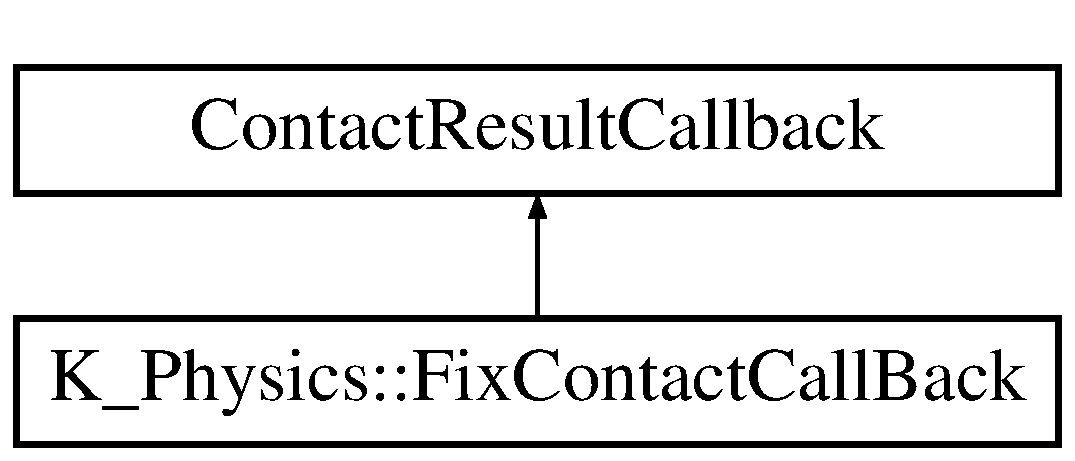
\includegraphics[height=2.000000cm]{struct_k___physics_1_1_fix_contact_call_back}
\end{center}
\end{figure}
\subsection*{公開メンバ関数}
\begin{DoxyCompactItemize}
\item 
\mbox{\hyperlink{struct_k___physics_1_1_fix_contact_call_back_aaa5c9013bf57d2196b55654bcdf360d3}{Fix\+Contact\+Call\+Back}} (bt\+Collision\+Object $\ast$\mbox{\hyperlink{struct_k___physics_1_1_fix_contact_call_back_ae632dff95a587e5cb73f5bbadf290a83}{obj}})
\item 
virtual bt\+Scalar \mbox{\hyperlink{struct_k___physics_1_1_fix_contact_call_back_ad6f9dd66fd4b001dfd4b687c18c16021}{add\+Single\+Result}} (bt\+Manifold\+Point \&cp, const bt\+Collision\+Object\+Wrapper $\ast$col\+Obj0\+Wrap, int part\+Id0, int index0, const bt\+Collision\+Object\+Wrapper $\ast$col\+Obj1\+Wrap, int part\+Id1, int index1)
\end{DoxyCompactItemize}
\subsection*{公開変数類}
\begin{DoxyCompactItemize}
\item 
bt\+Collision\+Object $\ast$ \mbox{\hyperlink{struct_k___physics_1_1_fix_contact_call_back_ae632dff95a587e5cb73f5bbadf290a83}{obj}}
\item 
float \mbox{\hyperlink{struct_k___physics_1_1_fix_contact_call_back_aba34225ba4a8474eaf9b22e9c18a1918}{max\+Distance}}
\item 
bt\+Vector3 \mbox{\hyperlink{struct_k___physics_1_1_fix_contact_call_back_a77ff8a19e7dff813ffc0831d03486411}{fix\+Vec}}
\item 
int \mbox{\hyperlink{struct_k___physics_1_1_fix_contact_call_back_a38ab6408dd65772d2db8ac20435cd4ec}{count}}
\item 
bool \mbox{\hyperlink{struct_k___physics_1_1_fix_contact_call_back_a0937fcc52b102eda9fc569acbff386c1}{is\+Loop}}
\end{DoxyCompactItemize}


\subsection{構築子と解体子}
\mbox{\Hypertarget{struct_k___physics_1_1_fix_contact_call_back_aaa5c9013bf57d2196b55654bcdf360d3}\label{struct_k___physics_1_1_fix_contact_call_back_aaa5c9013bf57d2196b55654bcdf360d3}} 
\index{K\+\_\+\+Physics\+::\+Fix\+Contact\+Call\+Back@{K\+\_\+\+Physics\+::\+Fix\+Contact\+Call\+Back}!Fix\+Contact\+Call\+Back@{Fix\+Contact\+Call\+Back}}
\index{Fix\+Contact\+Call\+Back@{Fix\+Contact\+Call\+Back}!K\+\_\+\+Physics\+::\+Fix\+Contact\+Call\+Back@{K\+\_\+\+Physics\+::\+Fix\+Contact\+Call\+Back}}
\subsubsection{\texorpdfstring{Fix\+Contact\+Call\+Back()}{FixContactCallBack()}}
{\footnotesize\ttfamily K\+\_\+\+Physics\+::\+Fix\+Contact\+Call\+Back\+::\+Fix\+Contact\+Call\+Back (\begin{DoxyParamCaption}\item[{bt\+Collision\+Object $\ast$}]{obj }\end{DoxyParamCaption})}



\subsection{関数詳解}
\mbox{\Hypertarget{struct_k___physics_1_1_fix_contact_call_back_ad6f9dd66fd4b001dfd4b687c18c16021}\label{struct_k___physics_1_1_fix_contact_call_back_ad6f9dd66fd4b001dfd4b687c18c16021}} 
\index{K\+\_\+\+Physics\+::\+Fix\+Contact\+Call\+Back@{K\+\_\+\+Physics\+::\+Fix\+Contact\+Call\+Back}!add\+Single\+Result@{add\+Single\+Result}}
\index{add\+Single\+Result@{add\+Single\+Result}!K\+\_\+\+Physics\+::\+Fix\+Contact\+Call\+Back@{K\+\_\+\+Physics\+::\+Fix\+Contact\+Call\+Back}}
\subsubsection{\texorpdfstring{add\+Single\+Result()}{addSingleResult()}}
{\footnotesize\ttfamily bt\+Scalar K\+\_\+\+Physics\+::\+Fix\+Contact\+Call\+Back\+::add\+Single\+Result (\begin{DoxyParamCaption}\item[{bt\+Manifold\+Point \&}]{cp,  }\item[{const bt\+Collision\+Object\+Wrapper $\ast$}]{col\+Obj0\+Wrap,  }\item[{int}]{part\+Id0,  }\item[{int}]{index0,  }\item[{const bt\+Collision\+Object\+Wrapper $\ast$}]{col\+Obj1\+Wrap,  }\item[{int}]{part\+Id1,  }\item[{int}]{index1 }\end{DoxyParamCaption})\hspace{0.3cm}{\ttfamily [virtual]}}



\subsection{メンバ詳解}
\mbox{\Hypertarget{struct_k___physics_1_1_fix_contact_call_back_a38ab6408dd65772d2db8ac20435cd4ec}\label{struct_k___physics_1_1_fix_contact_call_back_a38ab6408dd65772d2db8ac20435cd4ec}} 
\index{K\+\_\+\+Physics\+::\+Fix\+Contact\+Call\+Back@{K\+\_\+\+Physics\+::\+Fix\+Contact\+Call\+Back}!count@{count}}
\index{count@{count}!K\+\_\+\+Physics\+::\+Fix\+Contact\+Call\+Back@{K\+\_\+\+Physics\+::\+Fix\+Contact\+Call\+Back}}
\subsubsection{\texorpdfstring{count}{count}}
{\footnotesize\ttfamily int K\+\_\+\+Physics\+::\+Fix\+Contact\+Call\+Back\+::count}

\mbox{\Hypertarget{struct_k___physics_1_1_fix_contact_call_back_a77ff8a19e7dff813ffc0831d03486411}\label{struct_k___physics_1_1_fix_contact_call_back_a77ff8a19e7dff813ffc0831d03486411}} 
\index{K\+\_\+\+Physics\+::\+Fix\+Contact\+Call\+Back@{K\+\_\+\+Physics\+::\+Fix\+Contact\+Call\+Back}!fix\+Vec@{fix\+Vec}}
\index{fix\+Vec@{fix\+Vec}!K\+\_\+\+Physics\+::\+Fix\+Contact\+Call\+Back@{K\+\_\+\+Physics\+::\+Fix\+Contact\+Call\+Back}}
\subsubsection{\texorpdfstring{fix\+Vec}{fixVec}}
{\footnotesize\ttfamily bt\+Vector3 K\+\_\+\+Physics\+::\+Fix\+Contact\+Call\+Back\+::fix\+Vec}

\mbox{\Hypertarget{struct_k___physics_1_1_fix_contact_call_back_a0937fcc52b102eda9fc569acbff386c1}\label{struct_k___physics_1_1_fix_contact_call_back_a0937fcc52b102eda9fc569acbff386c1}} 
\index{K\+\_\+\+Physics\+::\+Fix\+Contact\+Call\+Back@{K\+\_\+\+Physics\+::\+Fix\+Contact\+Call\+Back}!is\+Loop@{is\+Loop}}
\index{is\+Loop@{is\+Loop}!K\+\_\+\+Physics\+::\+Fix\+Contact\+Call\+Back@{K\+\_\+\+Physics\+::\+Fix\+Contact\+Call\+Back}}
\subsubsection{\texorpdfstring{is\+Loop}{isLoop}}
{\footnotesize\ttfamily bool K\+\_\+\+Physics\+::\+Fix\+Contact\+Call\+Back\+::is\+Loop}

\mbox{\Hypertarget{struct_k___physics_1_1_fix_contact_call_back_aba34225ba4a8474eaf9b22e9c18a1918}\label{struct_k___physics_1_1_fix_contact_call_back_aba34225ba4a8474eaf9b22e9c18a1918}} 
\index{K\+\_\+\+Physics\+::\+Fix\+Contact\+Call\+Back@{K\+\_\+\+Physics\+::\+Fix\+Contact\+Call\+Back}!max\+Distance@{max\+Distance}}
\index{max\+Distance@{max\+Distance}!K\+\_\+\+Physics\+::\+Fix\+Contact\+Call\+Back@{K\+\_\+\+Physics\+::\+Fix\+Contact\+Call\+Back}}
\subsubsection{\texorpdfstring{max\+Distance}{maxDistance}}
{\footnotesize\ttfamily float K\+\_\+\+Physics\+::\+Fix\+Contact\+Call\+Back\+::max\+Distance}

\mbox{\Hypertarget{struct_k___physics_1_1_fix_contact_call_back_ae632dff95a587e5cb73f5bbadf290a83}\label{struct_k___physics_1_1_fix_contact_call_back_ae632dff95a587e5cb73f5bbadf290a83}} 
\index{K\+\_\+\+Physics\+::\+Fix\+Contact\+Call\+Back@{K\+\_\+\+Physics\+::\+Fix\+Contact\+Call\+Back}!obj@{obj}}
\index{obj@{obj}!K\+\_\+\+Physics\+::\+Fix\+Contact\+Call\+Back@{K\+\_\+\+Physics\+::\+Fix\+Contact\+Call\+Back}}
\subsubsection{\texorpdfstring{obj}{obj}}
{\footnotesize\ttfamily bt\+Collision\+Object$\ast$ K\+\_\+\+Physics\+::\+Fix\+Contact\+Call\+Back\+::obj}


\hypertarget{struct_k___graphics_1_1_font_generator_1_1_font_atlas}{}\section{K\+\_\+\+Graphics\+:\+:Font\+Generator\+:\+:Font\+Atlas 構造体}
\label{struct_k___graphics_1_1_font_generator_1_1_font_atlas}\index{K\+\_\+\+Graphics\+::\+Font\+Generator\+::\+Font\+Atlas@{K\+\_\+\+Graphics\+::\+Font\+Generator\+::\+Font\+Atlas}}


{\ttfamily \#include $<$Font\+Generator.\+h$>$}

\subsection*{公開変数類}
\begin{DoxyCompactItemize}
\item 
\mbox{\hyperlink{class_k___graphics_1_1_texture}{Texture}} $\ast$ \mbox{\hyperlink{struct_k___graphics_1_1_font_generator_1_1_font_atlas_a8baa5f2223d8b7d2c941f8b25dbe8bbb}{texture}}
\item 
char $\ast$ \mbox{\hyperlink{struct_k___graphics_1_1_font_generator_1_1_font_atlas_af111ad1cbd008ffda2493d2dbbf19313}{buffer}}
\item 
unsigned int \mbox{\hyperlink{struct_k___graphics_1_1_font_generator_1_1_font_atlas_aec8f2bf718152b3d8cb804a6da87b76b}{width}}
\item 
unsigned int \mbox{\hyperlink{struct_k___graphics_1_1_font_generator_1_1_font_atlas_a1bca66a68215e07df7ddb1e3de90fff7}{height}}
\item 
unsigned int \mbox{\hyperlink{struct_k___graphics_1_1_font_generator_1_1_font_atlas_a1e7f96ad116e52c8f1f00c3df998931c}{texture\+Width}}
\item 
unsigned int \mbox{\hyperlink{struct_k___graphics_1_1_font_generator_1_1_font_atlas_a69fa52d8f8237fdd3fbe2e272bd7b832}{texture\+Height}}
\end{DoxyCompactItemize}


\subsection{メンバ詳解}
\mbox{\Hypertarget{struct_k___graphics_1_1_font_generator_1_1_font_atlas_af111ad1cbd008ffda2493d2dbbf19313}\label{struct_k___graphics_1_1_font_generator_1_1_font_atlas_af111ad1cbd008ffda2493d2dbbf19313}} 
\index{K\+\_\+\+Graphics\+::\+Font\+Generator\+::\+Font\+Atlas@{K\+\_\+\+Graphics\+::\+Font\+Generator\+::\+Font\+Atlas}!buffer@{buffer}}
\index{buffer@{buffer}!K\+\_\+\+Graphics\+::\+Font\+Generator\+::\+Font\+Atlas@{K\+\_\+\+Graphics\+::\+Font\+Generator\+::\+Font\+Atlas}}
\subsubsection{\texorpdfstring{buffer}{buffer}}
{\footnotesize\ttfamily char$\ast$ K\+\_\+\+Graphics\+::\+Font\+Generator\+::\+Font\+Atlas\+::buffer}

\mbox{\Hypertarget{struct_k___graphics_1_1_font_generator_1_1_font_atlas_a1bca66a68215e07df7ddb1e3de90fff7}\label{struct_k___graphics_1_1_font_generator_1_1_font_atlas_a1bca66a68215e07df7ddb1e3de90fff7}} 
\index{K\+\_\+\+Graphics\+::\+Font\+Generator\+::\+Font\+Atlas@{K\+\_\+\+Graphics\+::\+Font\+Generator\+::\+Font\+Atlas}!height@{height}}
\index{height@{height}!K\+\_\+\+Graphics\+::\+Font\+Generator\+::\+Font\+Atlas@{K\+\_\+\+Graphics\+::\+Font\+Generator\+::\+Font\+Atlas}}
\subsubsection{\texorpdfstring{height}{height}}
{\footnotesize\ttfamily unsigned int K\+\_\+\+Graphics\+::\+Font\+Generator\+::\+Font\+Atlas\+::height}

\mbox{\Hypertarget{struct_k___graphics_1_1_font_generator_1_1_font_atlas_a8baa5f2223d8b7d2c941f8b25dbe8bbb}\label{struct_k___graphics_1_1_font_generator_1_1_font_atlas_a8baa5f2223d8b7d2c941f8b25dbe8bbb}} 
\index{K\+\_\+\+Graphics\+::\+Font\+Generator\+::\+Font\+Atlas@{K\+\_\+\+Graphics\+::\+Font\+Generator\+::\+Font\+Atlas}!texture@{texture}}
\index{texture@{texture}!K\+\_\+\+Graphics\+::\+Font\+Generator\+::\+Font\+Atlas@{K\+\_\+\+Graphics\+::\+Font\+Generator\+::\+Font\+Atlas}}
\subsubsection{\texorpdfstring{texture}{texture}}
{\footnotesize\ttfamily \mbox{\hyperlink{class_k___graphics_1_1_texture}{Texture}}$\ast$ K\+\_\+\+Graphics\+::\+Font\+Generator\+::\+Font\+Atlas\+::texture}

\mbox{\Hypertarget{struct_k___graphics_1_1_font_generator_1_1_font_atlas_a69fa52d8f8237fdd3fbe2e272bd7b832}\label{struct_k___graphics_1_1_font_generator_1_1_font_atlas_a69fa52d8f8237fdd3fbe2e272bd7b832}} 
\index{K\+\_\+\+Graphics\+::\+Font\+Generator\+::\+Font\+Atlas@{K\+\_\+\+Graphics\+::\+Font\+Generator\+::\+Font\+Atlas}!texture\+Height@{texture\+Height}}
\index{texture\+Height@{texture\+Height}!K\+\_\+\+Graphics\+::\+Font\+Generator\+::\+Font\+Atlas@{K\+\_\+\+Graphics\+::\+Font\+Generator\+::\+Font\+Atlas}}
\subsubsection{\texorpdfstring{texture\+Height}{textureHeight}}
{\footnotesize\ttfamily unsigned int K\+\_\+\+Graphics\+::\+Font\+Generator\+::\+Font\+Atlas\+::texture\+Height}

\mbox{\Hypertarget{struct_k___graphics_1_1_font_generator_1_1_font_atlas_a1e7f96ad116e52c8f1f00c3df998931c}\label{struct_k___graphics_1_1_font_generator_1_1_font_atlas_a1e7f96ad116e52c8f1f00c3df998931c}} 
\index{K\+\_\+\+Graphics\+::\+Font\+Generator\+::\+Font\+Atlas@{K\+\_\+\+Graphics\+::\+Font\+Generator\+::\+Font\+Atlas}!texture\+Width@{texture\+Width}}
\index{texture\+Width@{texture\+Width}!K\+\_\+\+Graphics\+::\+Font\+Generator\+::\+Font\+Atlas@{K\+\_\+\+Graphics\+::\+Font\+Generator\+::\+Font\+Atlas}}
\subsubsection{\texorpdfstring{texture\+Width}{textureWidth}}
{\footnotesize\ttfamily unsigned int K\+\_\+\+Graphics\+::\+Font\+Generator\+::\+Font\+Atlas\+::texture\+Width}

\mbox{\Hypertarget{struct_k___graphics_1_1_font_generator_1_1_font_atlas_aec8f2bf718152b3d8cb804a6da87b76b}\label{struct_k___graphics_1_1_font_generator_1_1_font_atlas_aec8f2bf718152b3d8cb804a6da87b76b}} 
\index{K\+\_\+\+Graphics\+::\+Font\+Generator\+::\+Font\+Atlas@{K\+\_\+\+Graphics\+::\+Font\+Generator\+::\+Font\+Atlas}!width@{width}}
\index{width@{width}!K\+\_\+\+Graphics\+::\+Font\+Generator\+::\+Font\+Atlas@{K\+\_\+\+Graphics\+::\+Font\+Generator\+::\+Font\+Atlas}}
\subsubsection{\texorpdfstring{width}{width}}
{\footnotesize\ttfamily unsigned int K\+\_\+\+Graphics\+::\+Font\+Generator\+::\+Font\+Atlas\+::width}


\hypertarget{struct_k___graphics_1_1_font_generator_1_1_font_data}{}\section{K\+\_\+\+Graphics\+:\+:Font\+Generator\+:\+:Font\+Data 構造体}
\label{struct_k___graphics_1_1_font_generator_1_1_font_data}\index{K\+\_\+\+Graphics\+::\+Font\+Generator\+::\+Font\+Data@{K\+\_\+\+Graphics\+::\+Font\+Generator\+::\+Font\+Data}}


{\ttfamily \#include $<$Font\+Generator.\+h$>$}

\subsection*{公開変数類}
\begin{DoxyCompactItemize}
\item 
\mbox{\hyperlink{struct_k___math_1_1_box2_d}{K\+\_\+\+Math\+::\+Box2D}} \mbox{\hyperlink{struct_k___graphics_1_1_font_generator_1_1_font_data_a5e3be02902ccaca08f784d24c0c011a1}{location\+UV}}
\item 
int \mbox{\hyperlink{struct_k___graphics_1_1_font_generator_1_1_font_data_a495dfde57ef35cebf27f26723a9328a9}{fix\+PositionY}}
\item 
int \mbox{\hyperlink{struct_k___graphics_1_1_font_generator_1_1_font_data_a95a1bfc9d1f370cd3f639355c73c86a0}{advance}}
\end{DoxyCompactItemize}


\subsection{メンバ詳解}
\mbox{\Hypertarget{struct_k___graphics_1_1_font_generator_1_1_font_data_a95a1bfc9d1f370cd3f639355c73c86a0}\label{struct_k___graphics_1_1_font_generator_1_1_font_data_a95a1bfc9d1f370cd3f639355c73c86a0}} 
\index{K\+\_\+\+Graphics\+::\+Font\+Generator\+::\+Font\+Data@{K\+\_\+\+Graphics\+::\+Font\+Generator\+::\+Font\+Data}!advance@{advance}}
\index{advance@{advance}!K\+\_\+\+Graphics\+::\+Font\+Generator\+::\+Font\+Data@{K\+\_\+\+Graphics\+::\+Font\+Generator\+::\+Font\+Data}}
\subsubsection{\texorpdfstring{advance}{advance}}
{\footnotesize\ttfamily int K\+\_\+\+Graphics\+::\+Font\+Generator\+::\+Font\+Data\+::advance}

\mbox{\Hypertarget{struct_k___graphics_1_1_font_generator_1_1_font_data_a495dfde57ef35cebf27f26723a9328a9}\label{struct_k___graphics_1_1_font_generator_1_1_font_data_a495dfde57ef35cebf27f26723a9328a9}} 
\index{K\+\_\+\+Graphics\+::\+Font\+Generator\+::\+Font\+Data@{K\+\_\+\+Graphics\+::\+Font\+Generator\+::\+Font\+Data}!fix\+PositionY@{fix\+PositionY}}
\index{fix\+PositionY@{fix\+PositionY}!K\+\_\+\+Graphics\+::\+Font\+Generator\+::\+Font\+Data@{K\+\_\+\+Graphics\+::\+Font\+Generator\+::\+Font\+Data}}
\subsubsection{\texorpdfstring{fix\+PositionY}{fixPositionY}}
{\footnotesize\ttfamily int K\+\_\+\+Graphics\+::\+Font\+Generator\+::\+Font\+Data\+::fix\+PositionY}

\mbox{\Hypertarget{struct_k___graphics_1_1_font_generator_1_1_font_data_a5e3be02902ccaca08f784d24c0c011a1}\label{struct_k___graphics_1_1_font_generator_1_1_font_data_a5e3be02902ccaca08f784d24c0c011a1}} 
\index{K\+\_\+\+Graphics\+::\+Font\+Generator\+::\+Font\+Data@{K\+\_\+\+Graphics\+::\+Font\+Generator\+::\+Font\+Data}!location\+UV@{location\+UV}}
\index{location\+UV@{location\+UV}!K\+\_\+\+Graphics\+::\+Font\+Generator\+::\+Font\+Data@{K\+\_\+\+Graphics\+::\+Font\+Generator\+::\+Font\+Data}}
\subsubsection{\texorpdfstring{location\+UV}{locationUV}}
{\footnotesize\ttfamily \mbox{\hyperlink{struct_k___math_1_1_box2_d}{K\+\_\+\+Math\+::\+Box2D}} K\+\_\+\+Graphics\+::\+Font\+Generator\+::\+Font\+Data\+::location\+UV}


\hypertarget{class_k___graphics_1_1_font_generator}{}\section{K\+\_\+\+Graphics\+:\+:Font\+Generator クラス}
\label{class_k___graphics_1_1_font_generator}\index{K\+\_\+\+Graphics\+::\+Font\+Generator@{K\+\_\+\+Graphics\+::\+Font\+Generator}}


{\ttfamily \#include $<$Font\+Generator.\+h$>$}

\subsection*{クラス}
\begin{DoxyCompactItemize}
\item 
struct \mbox{\hyperlink{struct_k___graphics_1_1_font_generator_1_1_char_data}{Char\+Data}}
\item 
struct \mbox{\hyperlink{struct_k___graphics_1_1_font_generator_1_1_font_atlas}{Font\+Atlas}}
\item 
struct \mbox{\hyperlink{struct_k___graphics_1_1_font_generator_1_1_font_data}{Font\+Data}}
\end{DoxyCompactItemize}
\subsection*{公開メンバ関数}
\begin{DoxyCompactItemize}
\item 
\mbox{\hyperlink{class_k___graphics_1_1_font_generator_a832617f2e9d50a7c6c613fa701665901}{Font\+Generator}} (const char $\ast$font\+File\+Pass)
\item 
\mbox{\hyperlink{class_k___graphics_1_1_font_generator_ab79beb1d0cf1780577d5ea16c8d89d67}{$\sim$\+Font\+Generator}} ()
\item 
void \mbox{\hyperlink{class_k___graphics_1_1_font_generator_a012e42323f6a295173f63e9acfc82dfc}{Set\+Font}} (wchar\+\_\+t character, int font\+Size)
\item 
\mbox{\hyperlink{class_k___graphics_1_1_texture}{Texture}} $\ast$ \mbox{\hyperlink{class_k___graphics_1_1_font_generator_a2b5d1ab68fcf0ffe83c65f4c694628bc}{Get\+Font\+Atlas}} (int font\+Size)
\item 
bool \mbox{\hyperlink{class_k___graphics_1_1_font_generator_ae6260c5ee857b4b95dc341d2160b1d6d}{Get\+Font\+Data}} (\mbox{\hyperlink{struct_k___graphics_1_1_font_generator_1_1_font_data}{Font\+Data}} \&result, wchar\+\_\+t font, int font\+Size)
\item 
void \mbox{\hyperlink{class_k___graphics_1_1_font_generator_ae84e22ce5a6e38d03f77f8a3b9393012}{Clear\+Font\+Atlas}} (int font\+Size)
\item 
void \mbox{\hyperlink{class_k___graphics_1_1_font_generator_a2e90321835a229436d378647aaddcab5}{Clear\+All\+Font\+Atlas}} ()
\end{DoxyCompactItemize}


\subsection{構築子と解体子}
\mbox{\Hypertarget{class_k___graphics_1_1_font_generator_a832617f2e9d50a7c6c613fa701665901}\label{class_k___graphics_1_1_font_generator_a832617f2e9d50a7c6c613fa701665901}} 
\index{K\+\_\+\+Graphics\+::\+Font\+Generator@{K\+\_\+\+Graphics\+::\+Font\+Generator}!Font\+Generator@{Font\+Generator}}
\index{Font\+Generator@{Font\+Generator}!K\+\_\+\+Graphics\+::\+Font\+Generator@{K\+\_\+\+Graphics\+::\+Font\+Generator}}
\subsubsection{\texorpdfstring{Font\+Generator()}{FontGenerator()}}
{\footnotesize\ttfamily K\+\_\+\+Graphics\+::\+Font\+Generator\+::\+Font\+Generator (\begin{DoxyParamCaption}\item[{const char $\ast$}]{font\+File\+Pass }\end{DoxyParamCaption})}

\mbox{\Hypertarget{class_k___graphics_1_1_font_generator_ab79beb1d0cf1780577d5ea16c8d89d67}\label{class_k___graphics_1_1_font_generator_ab79beb1d0cf1780577d5ea16c8d89d67}} 
\index{K\+\_\+\+Graphics\+::\+Font\+Generator@{K\+\_\+\+Graphics\+::\+Font\+Generator}!````~Font\+Generator@{$\sim$\+Font\+Generator}}
\index{````~Font\+Generator@{$\sim$\+Font\+Generator}!K\+\_\+\+Graphics\+::\+Font\+Generator@{K\+\_\+\+Graphics\+::\+Font\+Generator}}
\subsubsection{\texorpdfstring{$\sim$\+Font\+Generator()}{~FontGenerator()}}
{\footnotesize\ttfamily K\+\_\+\+Graphics\+::\+Font\+Generator\+::$\sim$\+Font\+Generator (\begin{DoxyParamCaption}{ }\end{DoxyParamCaption})}



\subsection{関数詳解}
\mbox{\Hypertarget{class_k___graphics_1_1_font_generator_a2e90321835a229436d378647aaddcab5}\label{class_k___graphics_1_1_font_generator_a2e90321835a229436d378647aaddcab5}} 
\index{K\+\_\+\+Graphics\+::\+Font\+Generator@{K\+\_\+\+Graphics\+::\+Font\+Generator}!Clear\+All\+Font\+Atlas@{Clear\+All\+Font\+Atlas}}
\index{Clear\+All\+Font\+Atlas@{Clear\+All\+Font\+Atlas}!K\+\_\+\+Graphics\+::\+Font\+Generator@{K\+\_\+\+Graphics\+::\+Font\+Generator}}
\subsubsection{\texorpdfstring{Clear\+All\+Font\+Atlas()}{ClearAllFontAtlas()}}
{\footnotesize\ttfamily void K\+\_\+\+Graphics\+::\+Font\+Generator\+::\+Clear\+All\+Font\+Atlas (\begin{DoxyParamCaption}{ }\end{DoxyParamCaption})}

\mbox{\Hypertarget{class_k___graphics_1_1_font_generator_ae84e22ce5a6e38d03f77f8a3b9393012}\label{class_k___graphics_1_1_font_generator_ae84e22ce5a6e38d03f77f8a3b9393012}} 
\index{K\+\_\+\+Graphics\+::\+Font\+Generator@{K\+\_\+\+Graphics\+::\+Font\+Generator}!Clear\+Font\+Atlas@{Clear\+Font\+Atlas}}
\index{Clear\+Font\+Atlas@{Clear\+Font\+Atlas}!K\+\_\+\+Graphics\+::\+Font\+Generator@{K\+\_\+\+Graphics\+::\+Font\+Generator}}
\subsubsection{\texorpdfstring{Clear\+Font\+Atlas()}{ClearFontAtlas()}}
{\footnotesize\ttfamily void K\+\_\+\+Graphics\+::\+Font\+Generator\+::\+Clear\+Font\+Atlas (\begin{DoxyParamCaption}\item[{int}]{font\+Size }\end{DoxyParamCaption})}

\mbox{\Hypertarget{class_k___graphics_1_1_font_generator_a2b5d1ab68fcf0ffe83c65f4c694628bc}\label{class_k___graphics_1_1_font_generator_a2b5d1ab68fcf0ffe83c65f4c694628bc}} 
\index{K\+\_\+\+Graphics\+::\+Font\+Generator@{K\+\_\+\+Graphics\+::\+Font\+Generator}!Get\+Font\+Atlas@{Get\+Font\+Atlas}}
\index{Get\+Font\+Atlas@{Get\+Font\+Atlas}!K\+\_\+\+Graphics\+::\+Font\+Generator@{K\+\_\+\+Graphics\+::\+Font\+Generator}}
\subsubsection{\texorpdfstring{Get\+Font\+Atlas()}{GetFontAtlas()}}
{\footnotesize\ttfamily \mbox{\hyperlink{class_k___graphics_1_1_texture}{Texture}} $\ast$ K\+\_\+\+Graphics\+::\+Font\+Generator\+::\+Get\+Font\+Atlas (\begin{DoxyParamCaption}\item[{int}]{font\+Size }\end{DoxyParamCaption})}

\mbox{\Hypertarget{class_k___graphics_1_1_font_generator_ae6260c5ee857b4b95dc341d2160b1d6d}\label{class_k___graphics_1_1_font_generator_ae6260c5ee857b4b95dc341d2160b1d6d}} 
\index{K\+\_\+\+Graphics\+::\+Font\+Generator@{K\+\_\+\+Graphics\+::\+Font\+Generator}!Get\+Font\+Data@{Get\+Font\+Data}}
\index{Get\+Font\+Data@{Get\+Font\+Data}!K\+\_\+\+Graphics\+::\+Font\+Generator@{K\+\_\+\+Graphics\+::\+Font\+Generator}}
\subsubsection{\texorpdfstring{Get\+Font\+Data()}{GetFontData()}}
{\footnotesize\ttfamily bool K\+\_\+\+Graphics\+::\+Font\+Generator\+::\+Get\+Font\+Data (\begin{DoxyParamCaption}\item[{\mbox{\hyperlink{struct_k___graphics_1_1_font_generator_1_1_font_data}{Font\+Data}} \&}]{result,  }\item[{wchar\+\_\+t}]{font,  }\item[{int}]{font\+Size }\end{DoxyParamCaption})}

\mbox{\Hypertarget{class_k___graphics_1_1_font_generator_a012e42323f6a295173f63e9acfc82dfc}\label{class_k___graphics_1_1_font_generator_a012e42323f6a295173f63e9acfc82dfc}} 
\index{K\+\_\+\+Graphics\+::\+Font\+Generator@{K\+\_\+\+Graphics\+::\+Font\+Generator}!Set\+Font@{Set\+Font}}
\index{Set\+Font@{Set\+Font}!K\+\_\+\+Graphics\+::\+Font\+Generator@{K\+\_\+\+Graphics\+::\+Font\+Generator}}
\subsubsection{\texorpdfstring{Set\+Font()}{SetFont()}}
{\footnotesize\ttfamily void K\+\_\+\+Graphics\+::\+Font\+Generator\+::\+Set\+Font (\begin{DoxyParamCaption}\item[{wchar\+\_\+t}]{character,  }\item[{int}]{font\+Size }\end{DoxyParamCaption})}


\hypertarget{class_k___graphics_1_1_font_renderer}{}\section{K\+\_\+\+Graphics\+:\+:Font\+Renderer クラス}
\label{class_k___graphics_1_1_font_renderer}\index{K\+\_\+\+Graphics\+::\+Font\+Renderer@{K\+\_\+\+Graphics\+::\+Font\+Renderer}}


フォントを生成し、描画するクラス(ワイド文字列)  




{\ttfamily \#include $<$Font\+Renderer.\+h$>$}

\subsection*{公開メンバ関数}
\begin{DoxyCompactItemize}
\item 
\mbox{\hyperlink{class_k___graphics_1_1_font_renderer_a1c3ac227f5eb40934d5d5ea84c80c96b}{Font\+Renderer}} ()
\begin{DoxyCompactList}\small\item\em 描画に使用するスプライトを初期化 \end{DoxyCompactList}\item 
\mbox{\hyperlink{class_k___graphics_1_1_font_renderer_a0b3a9b0d7fa0e07342be6469e668b7cd}{$\sim$\+Font\+Renderer}} ()
\begin{DoxyCompactList}\small\item\em スプライトのポインタを開放 \end{DoxyCompactList}\item 
void \mbox{\hyperlink{class_k___graphics_1_1_font_renderer_a90ee7dabacdc9c324b6e422cd7402b89}{Draw}} (\mbox{\hyperlink{class_k___graphics_1_1_camera_class}{Camera\+Class}} $\ast$camera, \mbox{\hyperlink{class_k___graphics_1_1_shader_class}{Shader\+Class}} $\ast$shader)
\begin{DoxyCompactList}\small\item\em 事前に呼ばれた描画命令をここで行う \end{DoxyCompactList}\item 
bool \mbox{\hyperlink{class_k___graphics_1_1_font_renderer_a9fffd9b8ec36986810cfbaad1d58ab70}{Load\+Font}} (const char $\ast$font\+Name, const char $\ast$file\+Pass)
\begin{DoxyCompactList}\small\item\em フォントを読み込む \end{DoxyCompactList}\item 
bool \mbox{\hyperlink{class_k___graphics_1_1_font_renderer_afde212f8e56262e86ef01d12b2704dbd}{Set\+Cullent\+Font}} (const char $\ast$font\+Name)
\begin{DoxyCompactList}\small\item\em 使用するフォントを設定、失敗するとfalseを返し、セットされない \end{DoxyCompactList}\item 
void \mbox{\hyperlink{class_k___graphics_1_1_font_renderer_a8d3687d4a4dad3682ab2bfa29e9cc15b}{Draw\+String2D}} (const std\+::string \&text, int font\+Size, int posX, int posY)
\begin{DoxyCompactList}\small\item\em 指定座標からテキストの描画予約(位置はスクリーンの座標) \end{DoxyCompactList}\item 
void \mbox{\hyperlink{class_k___graphics_1_1_font_renderer_adfb9bb5d77fdcb2a52c5ce5b7f011a67}{Draw\+String3D}} (const std\+::string \&text, int font\+Size, float posX, float posY, float posZ)
\begin{DoxyCompactList}\small\item\em 指定座標からテキストの描画予約(位置は3\+D空間の座標) \end{DoxyCompactList}\item 
void \mbox{\hyperlink{class_k___graphics_1_1_font_renderer_ace5f43f6cbd1a5b18e41350ca2e64dea}{Clear\+Font\+Texture}} (int size)
\begin{DoxyCompactList}\small\item\em フォント描画に利用しているテクスチャを削除する \end{DoxyCompactList}\item 
void \mbox{\hyperlink{class_k___graphics_1_1_font_renderer_a7e75db1a4ddf8bb6c888ece135783673}{Clear\+All\+Font\+Texture}} ()
\begin{DoxyCompactList}\small\item\em フォント描画に利用しているテクスチャをすべて削除する \end{DoxyCompactList}\end{DoxyCompactItemize}


\subsection{詳解}
フォントを生成し、描画するクラス(ワイド文字列) 

\subsection{構築子と解体子}
\mbox{\Hypertarget{class_k___graphics_1_1_font_renderer_a1c3ac227f5eb40934d5d5ea84c80c96b}\label{class_k___graphics_1_1_font_renderer_a1c3ac227f5eb40934d5d5ea84c80c96b}} 
\index{K\+\_\+\+Graphics\+::\+Font\+Renderer@{K\+\_\+\+Graphics\+::\+Font\+Renderer}!Font\+Renderer@{Font\+Renderer}}
\index{Font\+Renderer@{Font\+Renderer}!K\+\_\+\+Graphics\+::\+Font\+Renderer@{K\+\_\+\+Graphics\+::\+Font\+Renderer}}
\subsubsection{\texorpdfstring{Font\+Renderer()}{FontRenderer()}}
{\footnotesize\ttfamily K\+\_\+\+Graphics\+::\+Font\+Renderer\+::\+Font\+Renderer (\begin{DoxyParamCaption}{ }\end{DoxyParamCaption})}



描画に使用するスプライトを初期化 

\mbox{\Hypertarget{class_k___graphics_1_1_font_renderer_a0b3a9b0d7fa0e07342be6469e668b7cd}\label{class_k___graphics_1_1_font_renderer_a0b3a9b0d7fa0e07342be6469e668b7cd}} 
\index{K\+\_\+\+Graphics\+::\+Font\+Renderer@{K\+\_\+\+Graphics\+::\+Font\+Renderer}!````~Font\+Renderer@{$\sim$\+Font\+Renderer}}
\index{````~Font\+Renderer@{$\sim$\+Font\+Renderer}!K\+\_\+\+Graphics\+::\+Font\+Renderer@{K\+\_\+\+Graphics\+::\+Font\+Renderer}}
\subsubsection{\texorpdfstring{$\sim$\+Font\+Renderer()}{~FontRenderer()}}
{\footnotesize\ttfamily K\+\_\+\+Graphics\+::\+Font\+Renderer\+::$\sim$\+Font\+Renderer (\begin{DoxyParamCaption}{ }\end{DoxyParamCaption})}



スプライトのポインタを開放 



\subsection{関数詳解}
\mbox{\Hypertarget{class_k___graphics_1_1_font_renderer_a7e75db1a4ddf8bb6c888ece135783673}\label{class_k___graphics_1_1_font_renderer_a7e75db1a4ddf8bb6c888ece135783673}} 
\index{K\+\_\+\+Graphics\+::\+Font\+Renderer@{K\+\_\+\+Graphics\+::\+Font\+Renderer}!Clear\+All\+Font\+Texture@{Clear\+All\+Font\+Texture}}
\index{Clear\+All\+Font\+Texture@{Clear\+All\+Font\+Texture}!K\+\_\+\+Graphics\+::\+Font\+Renderer@{K\+\_\+\+Graphics\+::\+Font\+Renderer}}
\subsubsection{\texorpdfstring{Clear\+All\+Font\+Texture()}{ClearAllFontTexture()}}
{\footnotesize\ttfamily void K\+\_\+\+Graphics\+::\+Font\+Renderer\+::\+Clear\+All\+Font\+Texture (\begin{DoxyParamCaption}{ }\end{DoxyParamCaption})}



フォント描画に利用しているテクスチャをすべて削除する 

\mbox{\Hypertarget{class_k___graphics_1_1_font_renderer_ace5f43f6cbd1a5b18e41350ca2e64dea}\label{class_k___graphics_1_1_font_renderer_ace5f43f6cbd1a5b18e41350ca2e64dea}} 
\index{K\+\_\+\+Graphics\+::\+Font\+Renderer@{K\+\_\+\+Graphics\+::\+Font\+Renderer}!Clear\+Font\+Texture@{Clear\+Font\+Texture}}
\index{Clear\+Font\+Texture@{Clear\+Font\+Texture}!K\+\_\+\+Graphics\+::\+Font\+Renderer@{K\+\_\+\+Graphics\+::\+Font\+Renderer}}
\subsubsection{\texorpdfstring{Clear\+Font\+Texture()}{ClearFontTexture()}}
{\footnotesize\ttfamily void K\+\_\+\+Graphics\+::\+Font\+Renderer\+::\+Clear\+Font\+Texture (\begin{DoxyParamCaption}\item[{int}]{size }\end{DoxyParamCaption})}



フォント描画に利用しているテクスチャを削除する 


\begin{DoxyParams}[1]{引数}
\mbox{\tt in}  & {\em size} & 削除するフォントのサイズ \\
\hline
\end{DoxyParams}
\mbox{\Hypertarget{class_k___graphics_1_1_font_renderer_a90ee7dabacdc9c324b6e422cd7402b89}\label{class_k___graphics_1_1_font_renderer_a90ee7dabacdc9c324b6e422cd7402b89}} 
\index{K\+\_\+\+Graphics\+::\+Font\+Renderer@{K\+\_\+\+Graphics\+::\+Font\+Renderer}!Draw@{Draw}}
\index{Draw@{Draw}!K\+\_\+\+Graphics\+::\+Font\+Renderer@{K\+\_\+\+Graphics\+::\+Font\+Renderer}}
\subsubsection{\texorpdfstring{Draw()}{Draw()}}
{\footnotesize\ttfamily void K\+\_\+\+Graphics\+::\+Font\+Renderer\+::\+Draw (\begin{DoxyParamCaption}\item[{\mbox{\hyperlink{class_k___graphics_1_1_camera_class}{Camera\+Class}} $\ast$}]{camera,  }\item[{\mbox{\hyperlink{class_k___graphics_1_1_shader_class}{Shader\+Class}} $\ast$}]{shader }\end{DoxyParamCaption})}



事前に呼ばれた描画命令をここで行う 


\begin{DoxyParams}[1]{引数}
\mbox{\tt in}  & {\em camera} & 使用するカメラ \\
\hline
\mbox{\tt in}  & {\em shader} & 使用するシェーダー(スプライトが描画できるもの) \\
\hline
\end{DoxyParams}
\mbox{\Hypertarget{class_k___graphics_1_1_font_renderer_a8d3687d4a4dad3682ab2bfa29e9cc15b}\label{class_k___graphics_1_1_font_renderer_a8d3687d4a4dad3682ab2bfa29e9cc15b}} 
\index{K\+\_\+\+Graphics\+::\+Font\+Renderer@{K\+\_\+\+Graphics\+::\+Font\+Renderer}!Draw\+String2D@{Draw\+String2D}}
\index{Draw\+String2D@{Draw\+String2D}!K\+\_\+\+Graphics\+::\+Font\+Renderer@{K\+\_\+\+Graphics\+::\+Font\+Renderer}}
\subsubsection{\texorpdfstring{Draw\+String2\+D()}{DrawString2D()}}
{\footnotesize\ttfamily void K\+\_\+\+Graphics\+::\+Font\+Renderer\+::\+Draw\+String2D (\begin{DoxyParamCaption}\item[{const std\+::string \&}]{text,  }\item[{int}]{font\+Size,  }\item[{int}]{posX,  }\item[{int}]{posY }\end{DoxyParamCaption})}



指定座標からテキストの描画予約(位置はスクリーンの座標) 


\begin{DoxyParams}[1]{引数}
\mbox{\tt in}  & {\em text} & 描画するテキスト \\
\hline
\mbox{\tt in}  & {\em font\+Size} & フォントのサイズ \\
\hline
\mbox{\tt in}  & {\em posX} & 描画座標 \\
\hline
\mbox{\tt in}  & {\em posY} & 描画座標 \\
\hline
\end{DoxyParams}
\mbox{\Hypertarget{class_k___graphics_1_1_font_renderer_adfb9bb5d77fdcb2a52c5ce5b7f011a67}\label{class_k___graphics_1_1_font_renderer_adfb9bb5d77fdcb2a52c5ce5b7f011a67}} 
\index{K\+\_\+\+Graphics\+::\+Font\+Renderer@{K\+\_\+\+Graphics\+::\+Font\+Renderer}!Draw\+String3D@{Draw\+String3D}}
\index{Draw\+String3D@{Draw\+String3D}!K\+\_\+\+Graphics\+::\+Font\+Renderer@{K\+\_\+\+Graphics\+::\+Font\+Renderer}}
\subsubsection{\texorpdfstring{Draw\+String3\+D()}{DrawString3D()}}
{\footnotesize\ttfamily void K\+\_\+\+Graphics\+::\+Font\+Renderer\+::\+Draw\+String3D (\begin{DoxyParamCaption}\item[{const std\+::string \&}]{text,  }\item[{int}]{font\+Size,  }\item[{float}]{posX,  }\item[{float}]{posY,  }\item[{float}]{posZ }\end{DoxyParamCaption})}



指定座標からテキストの描画予約(位置は3\+D空間の座標) 


\begin{DoxyParams}[1]{引数}
\mbox{\tt in}  & {\em text} & 描画するテキスト \\
\hline
\mbox{\tt in}  & {\em font\+Size} & フォントのサイズ \\
\hline
\mbox{\tt in}  & {\em posX} & 描画座標 \\
\hline
\mbox{\tt in}  & {\em posY} & 描画座標 \\
\hline
\mbox{\tt in}  & {\em posZ} & 描画座標 \\
\hline
\end{DoxyParams}
\mbox{\Hypertarget{class_k___graphics_1_1_font_renderer_a9fffd9b8ec36986810cfbaad1d58ab70}\label{class_k___graphics_1_1_font_renderer_a9fffd9b8ec36986810cfbaad1d58ab70}} 
\index{K\+\_\+\+Graphics\+::\+Font\+Renderer@{K\+\_\+\+Graphics\+::\+Font\+Renderer}!Load\+Font@{Load\+Font}}
\index{Load\+Font@{Load\+Font}!K\+\_\+\+Graphics\+::\+Font\+Renderer@{K\+\_\+\+Graphics\+::\+Font\+Renderer}}
\subsubsection{\texorpdfstring{Load\+Font()}{LoadFont()}}
{\footnotesize\ttfamily bool K\+\_\+\+Graphics\+::\+Font\+Renderer\+::\+Load\+Font (\begin{DoxyParamCaption}\item[{const char $\ast$}]{font\+Name,  }\item[{const char $\ast$}]{file\+Pass }\end{DoxyParamCaption})}



フォントを読み込む 


\begin{DoxyParams}[1]{引数}
\mbox{\tt in}  & {\em font\+Name} & フォントのユーザー定義名 \\
\hline
\mbox{\tt in}  & {\em file\+Pass} & フォントのファイルパス \\
\hline
\end{DoxyParams}
\mbox{\Hypertarget{class_k___graphics_1_1_font_renderer_afde212f8e56262e86ef01d12b2704dbd}\label{class_k___graphics_1_1_font_renderer_afde212f8e56262e86ef01d12b2704dbd}} 
\index{K\+\_\+\+Graphics\+::\+Font\+Renderer@{K\+\_\+\+Graphics\+::\+Font\+Renderer}!Set\+Cullent\+Font@{Set\+Cullent\+Font}}
\index{Set\+Cullent\+Font@{Set\+Cullent\+Font}!K\+\_\+\+Graphics\+::\+Font\+Renderer@{K\+\_\+\+Graphics\+::\+Font\+Renderer}}
\subsubsection{\texorpdfstring{Set\+Cullent\+Font()}{SetCullentFont()}}
{\footnotesize\ttfamily bool K\+\_\+\+Graphics\+::\+Font\+Renderer\+::\+Set\+Cullent\+Font (\begin{DoxyParamCaption}\item[{const char $\ast$}]{font\+Name }\end{DoxyParamCaption})}



使用するフォントを設定、失敗するとfalseを返し、セットされない 


\begin{DoxyParams}[1]{引数}
\mbox{\tt in}  & {\em font\+Name} & フォント名 \\
\hline
\end{DoxyParams}
\begin{DoxyReturn}{戻り値}
成功するとtrue 
\end{DoxyReturn}

\hypertarget{class_k___graphics_1_1_framebuffer}{}\section{K\+\_\+\+Graphics\+:\+:Framebuffer クラス}
\label{class_k___graphics_1_1_framebuffer}\index{K\+\_\+\+Graphics\+::\+Framebuffer@{K\+\_\+\+Graphics\+::\+Framebuffer}}


{\ttfamily \#include $<$Frame\+Buffer.\+h$>$}

\subsection*{公開メンバ関数}
\begin{DoxyCompactItemize}
\item 
\mbox{\hyperlink{class_k___graphics_1_1_framebuffer_a3f5d49c84ad44a44ca9878620d8b646d}{Framebuffer}} (\mbox{\hyperlink{class_k___graphics_1_1_texture}{Texture}} $\ast$texture, const std\+::string \&name)
\item 
\mbox{\hyperlink{class_k___graphics_1_1_framebuffer_a7c8f64070ecd55069b6964f1a5b48427}{Framebuffer}} (\mbox{\hyperlink{class_k___graphics_1_1_texture}{Texture}} $\ast$texture, const std\+::string \&name, G\+Luint depth\+Buffer)
\item 
\mbox{\hyperlink{class_k___graphics_1_1_framebuffer_ad3a492836b1ced0414f6b3aa4718097f}{$\sim$\+Framebuffer}} ()
\item 
bool \mbox{\hyperlink{class_k___graphics_1_1_framebuffer_a109152dd1cce45054686bcb1f6576528}{Initialize}} (\mbox{\hyperlink{class_k___graphics_1_1_texture}{Texture}} $\ast$texture, const std\+::string \&name, G\+Luint depth\+Buffer)
\item 
void \mbox{\hyperlink{class_k___graphics_1_1_framebuffer_adfc67359931e99fed0f3c2205dad593b}{Finalize}} ()
\item 
void \mbox{\hyperlink{class_k___graphics_1_1_framebuffer_afdbf1b4cf70c68149cd6c146d6a32687}{Bind}} ()
\item 
int \mbox{\hyperlink{class_k___graphics_1_1_framebuffer_a14bef34a3d986bca79cb0af59415bb3c}{Get\+Width}} ()
\item 
int \mbox{\hyperlink{class_k___graphics_1_1_framebuffer_aade734f04f110482729a7031f8b6301b}{Get\+Height}} ()
\item 
int \mbox{\hyperlink{class_k___graphics_1_1_framebuffer_a1f12c09991f4bb042206cd846b99b2ac}{Get\+Frame\+Buffer\+Handle}} ()
\item 
int \mbox{\hyperlink{class_k___graphics_1_1_framebuffer_aac0fa7173df91438b489cab5870e07eb}{Get\+Depth\+Buffer\+Handle}} ()
\end{DoxyCompactItemize}


\subsection{構築子と解体子}
\mbox{\Hypertarget{class_k___graphics_1_1_framebuffer_a3f5d49c84ad44a44ca9878620d8b646d}\label{class_k___graphics_1_1_framebuffer_a3f5d49c84ad44a44ca9878620d8b646d}} 
\index{K\+\_\+\+Graphics\+::\+Framebuffer@{K\+\_\+\+Graphics\+::\+Framebuffer}!Framebuffer@{Framebuffer}}
\index{Framebuffer@{Framebuffer}!K\+\_\+\+Graphics\+::\+Framebuffer@{K\+\_\+\+Graphics\+::\+Framebuffer}}
\subsubsection{\texorpdfstring{Framebuffer()}{Framebuffer()}\hspace{0.1cm}{\footnotesize\ttfamily [1/2]}}
{\footnotesize\ttfamily K\+\_\+\+Graphics\+::\+Framebuffer\+::\+Framebuffer (\begin{DoxyParamCaption}\item[{\mbox{\hyperlink{class_k___graphics_1_1_texture}{Texture}} $\ast$}]{texture,  }\item[{const std\+::string \&}]{name }\end{DoxyParamCaption})}

\mbox{\Hypertarget{class_k___graphics_1_1_framebuffer_a7c8f64070ecd55069b6964f1a5b48427}\label{class_k___graphics_1_1_framebuffer_a7c8f64070ecd55069b6964f1a5b48427}} 
\index{K\+\_\+\+Graphics\+::\+Framebuffer@{K\+\_\+\+Graphics\+::\+Framebuffer}!Framebuffer@{Framebuffer}}
\index{Framebuffer@{Framebuffer}!K\+\_\+\+Graphics\+::\+Framebuffer@{K\+\_\+\+Graphics\+::\+Framebuffer}}
\subsubsection{\texorpdfstring{Framebuffer()}{Framebuffer()}\hspace{0.1cm}{\footnotesize\ttfamily [2/2]}}
{\footnotesize\ttfamily K\+\_\+\+Graphics\+::\+Framebuffer\+::\+Framebuffer (\begin{DoxyParamCaption}\item[{\mbox{\hyperlink{class_k___graphics_1_1_texture}{Texture}} $\ast$}]{texture,  }\item[{const std\+::string \&}]{name,  }\item[{G\+Luint}]{depth\+Buffer }\end{DoxyParamCaption})}

\mbox{\Hypertarget{class_k___graphics_1_1_framebuffer_ad3a492836b1ced0414f6b3aa4718097f}\label{class_k___graphics_1_1_framebuffer_ad3a492836b1ced0414f6b3aa4718097f}} 
\index{K\+\_\+\+Graphics\+::\+Framebuffer@{K\+\_\+\+Graphics\+::\+Framebuffer}!````~Framebuffer@{$\sim$\+Framebuffer}}
\index{````~Framebuffer@{$\sim$\+Framebuffer}!K\+\_\+\+Graphics\+::\+Framebuffer@{K\+\_\+\+Graphics\+::\+Framebuffer}}
\subsubsection{\texorpdfstring{$\sim$\+Framebuffer()}{~Framebuffer()}}
{\footnotesize\ttfamily K\+\_\+\+Graphics\+::\+Framebuffer\+::$\sim$\+Framebuffer (\begin{DoxyParamCaption}{ }\end{DoxyParamCaption})}



\subsection{関数詳解}
\mbox{\Hypertarget{class_k___graphics_1_1_framebuffer_afdbf1b4cf70c68149cd6c146d6a32687}\label{class_k___graphics_1_1_framebuffer_afdbf1b4cf70c68149cd6c146d6a32687}} 
\index{K\+\_\+\+Graphics\+::\+Framebuffer@{K\+\_\+\+Graphics\+::\+Framebuffer}!Bind@{Bind}}
\index{Bind@{Bind}!K\+\_\+\+Graphics\+::\+Framebuffer@{K\+\_\+\+Graphics\+::\+Framebuffer}}
\subsubsection{\texorpdfstring{Bind()}{Bind()}}
{\footnotesize\ttfamily void K\+\_\+\+Graphics\+::\+Framebuffer\+::\+Bind (\begin{DoxyParamCaption}{ }\end{DoxyParamCaption})}

\mbox{\Hypertarget{class_k___graphics_1_1_framebuffer_adfc67359931e99fed0f3c2205dad593b}\label{class_k___graphics_1_1_framebuffer_adfc67359931e99fed0f3c2205dad593b}} 
\index{K\+\_\+\+Graphics\+::\+Framebuffer@{K\+\_\+\+Graphics\+::\+Framebuffer}!Finalize@{Finalize}}
\index{Finalize@{Finalize}!K\+\_\+\+Graphics\+::\+Framebuffer@{K\+\_\+\+Graphics\+::\+Framebuffer}}
\subsubsection{\texorpdfstring{Finalize()}{Finalize()}}
{\footnotesize\ttfamily void K\+\_\+\+Graphics\+::\+Framebuffer\+::\+Finalize (\begin{DoxyParamCaption}{ }\end{DoxyParamCaption})}

\mbox{\Hypertarget{class_k___graphics_1_1_framebuffer_aac0fa7173df91438b489cab5870e07eb}\label{class_k___graphics_1_1_framebuffer_aac0fa7173df91438b489cab5870e07eb}} 
\index{K\+\_\+\+Graphics\+::\+Framebuffer@{K\+\_\+\+Graphics\+::\+Framebuffer}!Get\+Depth\+Buffer\+Handle@{Get\+Depth\+Buffer\+Handle}}
\index{Get\+Depth\+Buffer\+Handle@{Get\+Depth\+Buffer\+Handle}!K\+\_\+\+Graphics\+::\+Framebuffer@{K\+\_\+\+Graphics\+::\+Framebuffer}}
\subsubsection{\texorpdfstring{Get\+Depth\+Buffer\+Handle()}{GetDepthBufferHandle()}}
{\footnotesize\ttfamily int K\+\_\+\+Graphics\+::\+Framebuffer\+::\+Get\+Depth\+Buffer\+Handle (\begin{DoxyParamCaption}{ }\end{DoxyParamCaption})}

\mbox{\Hypertarget{class_k___graphics_1_1_framebuffer_a1f12c09991f4bb042206cd846b99b2ac}\label{class_k___graphics_1_1_framebuffer_a1f12c09991f4bb042206cd846b99b2ac}} 
\index{K\+\_\+\+Graphics\+::\+Framebuffer@{K\+\_\+\+Graphics\+::\+Framebuffer}!Get\+Frame\+Buffer\+Handle@{Get\+Frame\+Buffer\+Handle}}
\index{Get\+Frame\+Buffer\+Handle@{Get\+Frame\+Buffer\+Handle}!K\+\_\+\+Graphics\+::\+Framebuffer@{K\+\_\+\+Graphics\+::\+Framebuffer}}
\subsubsection{\texorpdfstring{Get\+Frame\+Buffer\+Handle()}{GetFrameBufferHandle()}}
{\footnotesize\ttfamily int K\+\_\+\+Graphics\+::\+Framebuffer\+::\+Get\+Frame\+Buffer\+Handle (\begin{DoxyParamCaption}{ }\end{DoxyParamCaption})}

\mbox{\Hypertarget{class_k___graphics_1_1_framebuffer_aade734f04f110482729a7031f8b6301b}\label{class_k___graphics_1_1_framebuffer_aade734f04f110482729a7031f8b6301b}} 
\index{K\+\_\+\+Graphics\+::\+Framebuffer@{K\+\_\+\+Graphics\+::\+Framebuffer}!Get\+Height@{Get\+Height}}
\index{Get\+Height@{Get\+Height}!K\+\_\+\+Graphics\+::\+Framebuffer@{K\+\_\+\+Graphics\+::\+Framebuffer}}
\subsubsection{\texorpdfstring{Get\+Height()}{GetHeight()}}
{\footnotesize\ttfamily int K\+\_\+\+Graphics\+::\+Framebuffer\+::\+Get\+Height (\begin{DoxyParamCaption}{ }\end{DoxyParamCaption})}

\mbox{\Hypertarget{class_k___graphics_1_1_framebuffer_a14bef34a3d986bca79cb0af59415bb3c}\label{class_k___graphics_1_1_framebuffer_a14bef34a3d986bca79cb0af59415bb3c}} 
\index{K\+\_\+\+Graphics\+::\+Framebuffer@{K\+\_\+\+Graphics\+::\+Framebuffer}!Get\+Width@{Get\+Width}}
\index{Get\+Width@{Get\+Width}!K\+\_\+\+Graphics\+::\+Framebuffer@{K\+\_\+\+Graphics\+::\+Framebuffer}}
\subsubsection{\texorpdfstring{Get\+Width()}{GetWidth()}}
{\footnotesize\ttfamily int K\+\_\+\+Graphics\+::\+Framebuffer\+::\+Get\+Width (\begin{DoxyParamCaption}{ }\end{DoxyParamCaption})}

\mbox{\Hypertarget{class_k___graphics_1_1_framebuffer_a109152dd1cce45054686bcb1f6576528}\label{class_k___graphics_1_1_framebuffer_a109152dd1cce45054686bcb1f6576528}} 
\index{K\+\_\+\+Graphics\+::\+Framebuffer@{K\+\_\+\+Graphics\+::\+Framebuffer}!Initialize@{Initialize}}
\index{Initialize@{Initialize}!K\+\_\+\+Graphics\+::\+Framebuffer@{K\+\_\+\+Graphics\+::\+Framebuffer}}
\subsubsection{\texorpdfstring{Initialize()}{Initialize()}}
{\footnotesize\ttfamily bool K\+\_\+\+Graphics\+::\+Framebuffer\+::\+Initialize (\begin{DoxyParamCaption}\item[{\mbox{\hyperlink{class_k___graphics_1_1_texture}{Texture}} $\ast$}]{texture,  }\item[{const std\+::string \&}]{name,  }\item[{G\+Luint}]{depth\+Buffer }\end{DoxyParamCaption})}


\hypertarget{class_k___graphics_1_1_frame_buffer_list}{}\section{K\+\_\+\+Graphics\+:\+:Frame\+Buffer\+List クラス}
\label{class_k___graphics_1_1_frame_buffer_list}\index{K\+\_\+\+Graphics\+::\+Frame\+Buffer\+List@{K\+\_\+\+Graphics\+::\+Frame\+Buffer\+List}}


{\ttfamily \#include $<$Frame\+Buffer\+List.\+h$>$}

\subsection*{公開メンバ関数}
\begin{DoxyCompactItemize}
\item 
\mbox{\hyperlink{class_k___graphics_1_1_frame_buffer_list_adde18222008a5b4d2962b6432c9eea4f}{Frame\+Buffer\+List}} (\mbox{\hyperlink{class_k___graphics_1_1_texture_list}{Texture\+List}} $\ast$list)
\begin{DoxyCompactList}\small\item\em テクスチャリストへのポインタを渡して初期化 \end{DoxyCompactList}\item 
\mbox{\hyperlink{class_k___graphics_1_1_frame_buffer_list_a0e7f1925dd1ae7b506cab0d023438552}{$\sim$\+Frame\+Buffer\+List}} ()
\begin{DoxyCompactList}\small\item\em 終了処理をする \end{DoxyCompactList}\item 
bool \mbox{\hyperlink{class_k___graphics_1_1_frame_buffer_list_a21a4bff7e956835548565d9b46c031b5}{Create\+Frame\+Buffer}} (const std\+::string \&name, int width, int height)
\begin{DoxyCompactList}\small\item\em テクスチャリストに新規作成を依頼し、フレームバッファ作成&リスト登録 深度バッファを使いまわすときはそのフレームバッファの名前を引数に渡す \end{DoxyCompactList}\item 
bool \mbox{\hyperlink{class_k___graphics_1_1_frame_buffer_list_a0ba074b9922c099102a43e92b6815d4c}{Create\+Frame\+Buffer}} (const std\+::string \&name, const std\+::string \&depth\+Buffer, int width, int height)
\begin{DoxyCompactList}\small\item\em テクスチャリストに新規作成を依頼し、フレームバッファ作成&リスト登録 深度バッファを使いまわすときはそのフレームバッファの名前を引数に渡す \end{DoxyCompactList}\item 
void \mbox{\hyperlink{class_k___graphics_1_1_frame_buffer_list_a2f45d6dd0bc044ebcbd2e2cd58b6786f}{Begin\+Draw}} (const std\+::string \&name, float r, float g, float b, bool not\+Delete\+Depth\+Stencil=false)
\begin{DoxyCompactList}\small\item\em 指定色でフレームバッファをクリアする \end{DoxyCompactList}\item 
void \mbox{\hyperlink{class_k___graphics_1_1_frame_buffer_list_aa850bab5299917ccd10a4f90439c733d}{Begin\+Draw}} (int view\+Port\+Width, int view\+Port\+Height, float r, float g, float b, bool not\+Delete\+Depth\+Stencil=false)
\begin{DoxyCompactList}\small\item\em ビューポートを設定し、指定色でバックバッファをクリアする \end{DoxyCompactList}\item 
void \mbox{\hyperlink{class_k___graphics_1_1_frame_buffer_list_a34e1278edf425c32aefd3e2684886930}{End\+Draw}} ()
\begin{DoxyCompactList}\small\item\em バインドを解いて描画終了 \end{DoxyCompactList}\end{DoxyCompactItemize}


\subsection{構築子と解体子}
\mbox{\Hypertarget{class_k___graphics_1_1_frame_buffer_list_adde18222008a5b4d2962b6432c9eea4f}\label{class_k___graphics_1_1_frame_buffer_list_adde18222008a5b4d2962b6432c9eea4f}} 
\index{K\+\_\+\+Graphics\+::\+Frame\+Buffer\+List@{K\+\_\+\+Graphics\+::\+Frame\+Buffer\+List}!Frame\+Buffer\+List@{Frame\+Buffer\+List}}
\index{Frame\+Buffer\+List@{Frame\+Buffer\+List}!K\+\_\+\+Graphics\+::\+Frame\+Buffer\+List@{K\+\_\+\+Graphics\+::\+Frame\+Buffer\+List}}
\subsubsection{\texorpdfstring{Frame\+Buffer\+List()}{FrameBufferList()}}
{\footnotesize\ttfamily K\+\_\+\+Graphics\+::\+Frame\+Buffer\+List\+::\+Frame\+Buffer\+List (\begin{DoxyParamCaption}\item[{\mbox{\hyperlink{class_k___graphics_1_1_texture_list}{Texture\+List}} $\ast$}]{list }\end{DoxyParamCaption})}



テクスチャリストへのポインタを渡して初期化 

\mbox{\Hypertarget{class_k___graphics_1_1_frame_buffer_list_a0e7f1925dd1ae7b506cab0d023438552}\label{class_k___graphics_1_1_frame_buffer_list_a0e7f1925dd1ae7b506cab0d023438552}} 
\index{K\+\_\+\+Graphics\+::\+Frame\+Buffer\+List@{K\+\_\+\+Graphics\+::\+Frame\+Buffer\+List}!````~Frame\+Buffer\+List@{$\sim$\+Frame\+Buffer\+List}}
\index{````~Frame\+Buffer\+List@{$\sim$\+Frame\+Buffer\+List}!K\+\_\+\+Graphics\+::\+Frame\+Buffer\+List@{K\+\_\+\+Graphics\+::\+Frame\+Buffer\+List}}
\subsubsection{\texorpdfstring{$\sim$\+Frame\+Buffer\+List()}{~FrameBufferList()}}
{\footnotesize\ttfamily K\+\_\+\+Graphics\+::\+Frame\+Buffer\+List\+::$\sim$\+Frame\+Buffer\+List (\begin{DoxyParamCaption}{ }\end{DoxyParamCaption})}



終了処理をする 



\subsection{関数詳解}
\mbox{\Hypertarget{class_k___graphics_1_1_frame_buffer_list_a2f45d6dd0bc044ebcbd2e2cd58b6786f}\label{class_k___graphics_1_1_frame_buffer_list_a2f45d6dd0bc044ebcbd2e2cd58b6786f}} 
\index{K\+\_\+\+Graphics\+::\+Frame\+Buffer\+List@{K\+\_\+\+Graphics\+::\+Frame\+Buffer\+List}!Begin\+Draw@{Begin\+Draw}}
\index{Begin\+Draw@{Begin\+Draw}!K\+\_\+\+Graphics\+::\+Frame\+Buffer\+List@{K\+\_\+\+Graphics\+::\+Frame\+Buffer\+List}}
\subsubsection{\texorpdfstring{Begin\+Draw()}{BeginDraw()}\hspace{0.1cm}{\footnotesize\ttfamily [1/2]}}
{\footnotesize\ttfamily void K\+\_\+\+Graphics\+::\+Frame\+Buffer\+List\+::\+Begin\+Draw (\begin{DoxyParamCaption}\item[{const std\+::string \&}]{name,  }\item[{float}]{r,  }\item[{float}]{g,  }\item[{float}]{b,  }\item[{bool}]{not\+Delete\+Depth\+Stencil = {\ttfamily false} }\end{DoxyParamCaption})}



指定色でフレームバッファをクリアする 


\begin{DoxyParams}[1]{引数}
\mbox{\tt in}  & {\em name} & クリアするフレームバッファの名前 \\
\hline
\mbox{\tt in}  & {\em r} & クリア色の\+R成分 \\
\hline
\mbox{\tt in}  & {\em g} & クリア色の\+G成分 \\
\hline
\mbox{\tt in}  & {\em b} & クリア色の\+B成分 \\
\hline
\mbox{\tt in}  & {\em not\+Delete\+Depth\+Stencil} & trueにすると深度とステンシルをクリアしない(省略時false) \\
\hline
\end{DoxyParams}
\mbox{\Hypertarget{class_k___graphics_1_1_frame_buffer_list_aa850bab5299917ccd10a4f90439c733d}\label{class_k___graphics_1_1_frame_buffer_list_aa850bab5299917ccd10a4f90439c733d}} 
\index{K\+\_\+\+Graphics\+::\+Frame\+Buffer\+List@{K\+\_\+\+Graphics\+::\+Frame\+Buffer\+List}!Begin\+Draw@{Begin\+Draw}}
\index{Begin\+Draw@{Begin\+Draw}!K\+\_\+\+Graphics\+::\+Frame\+Buffer\+List@{K\+\_\+\+Graphics\+::\+Frame\+Buffer\+List}}
\subsubsection{\texorpdfstring{Begin\+Draw()}{BeginDraw()}\hspace{0.1cm}{\footnotesize\ttfamily [2/2]}}
{\footnotesize\ttfamily void K\+\_\+\+Graphics\+::\+Frame\+Buffer\+List\+::\+Begin\+Draw (\begin{DoxyParamCaption}\item[{int}]{view\+Port\+Width,  }\item[{int}]{view\+Port\+Height,  }\item[{float}]{r,  }\item[{float}]{g,  }\item[{float}]{b,  }\item[{bool}]{not\+Delete\+Depth\+Stencil = {\ttfamily false} }\end{DoxyParamCaption})}



ビューポートを設定し、指定色でバックバッファをクリアする 


\begin{DoxyParams}[1]{引数}
\mbox{\tt in}  & {\em view\+Port\+Width} & ビューポートの幅 \\
\hline
\mbox{\tt in}  & {\em view\+Port\+Height} & ビューポートの高さ \\
\hline
\mbox{\tt in}  & {\em r} & クリア色の\+R成分 \\
\hline
\mbox{\tt in}  & {\em g} & クリア色の\+G成分 \\
\hline
\mbox{\tt in}  & {\em b} & クリア色の\+B成分 \\
\hline
\mbox{\tt in}  & {\em not\+Delete\+Depth\+Stencil} & trueにすると深度とステンシルをクリアしない(省略時false) \\
\hline
\end{DoxyParams}
\mbox{\Hypertarget{class_k___graphics_1_1_frame_buffer_list_a21a4bff7e956835548565d9b46c031b5}\label{class_k___graphics_1_1_frame_buffer_list_a21a4bff7e956835548565d9b46c031b5}} 
\index{K\+\_\+\+Graphics\+::\+Frame\+Buffer\+List@{K\+\_\+\+Graphics\+::\+Frame\+Buffer\+List}!Create\+Frame\+Buffer@{Create\+Frame\+Buffer}}
\index{Create\+Frame\+Buffer@{Create\+Frame\+Buffer}!K\+\_\+\+Graphics\+::\+Frame\+Buffer\+List@{K\+\_\+\+Graphics\+::\+Frame\+Buffer\+List}}
\subsubsection{\texorpdfstring{Create\+Frame\+Buffer()}{CreateFrameBuffer()}\hspace{0.1cm}{\footnotesize\ttfamily [1/2]}}
{\footnotesize\ttfamily bool K\+\_\+\+Graphics\+::\+Frame\+Buffer\+List\+::\+Create\+Frame\+Buffer (\begin{DoxyParamCaption}\item[{const std\+::string \&}]{name,  }\item[{int}]{width,  }\item[{int}]{height }\end{DoxyParamCaption})}



テクスチャリストに新規作成を依頼し、フレームバッファ作成&リスト登録 深度バッファを使いまわすときはそのフレームバッファの名前を引数に渡す 


\begin{DoxyParams}[1]{引数}
\mbox{\tt in}  & {\em name} & 作成するフレームバッファのユーザー定義名 \\
\hline
\mbox{\tt in}  & {\em width} & 作成するフレームバッファのビューポート幅 \\
\hline
\mbox{\tt in}  & {\em height} & 作成するフレームバッファのビューポート高さ \\
\hline
\end{DoxyParams}
\mbox{\Hypertarget{class_k___graphics_1_1_frame_buffer_list_a0ba074b9922c099102a43e92b6815d4c}\label{class_k___graphics_1_1_frame_buffer_list_a0ba074b9922c099102a43e92b6815d4c}} 
\index{K\+\_\+\+Graphics\+::\+Frame\+Buffer\+List@{K\+\_\+\+Graphics\+::\+Frame\+Buffer\+List}!Create\+Frame\+Buffer@{Create\+Frame\+Buffer}}
\index{Create\+Frame\+Buffer@{Create\+Frame\+Buffer}!K\+\_\+\+Graphics\+::\+Frame\+Buffer\+List@{K\+\_\+\+Graphics\+::\+Frame\+Buffer\+List}}
\subsubsection{\texorpdfstring{Create\+Frame\+Buffer()}{CreateFrameBuffer()}\hspace{0.1cm}{\footnotesize\ttfamily [2/2]}}
{\footnotesize\ttfamily bool K\+\_\+\+Graphics\+::\+Frame\+Buffer\+List\+::\+Create\+Frame\+Buffer (\begin{DoxyParamCaption}\item[{const std\+::string \&}]{name,  }\item[{const std\+::string \&}]{depth\+Buffer,  }\item[{int}]{width,  }\item[{int}]{height }\end{DoxyParamCaption})}



テクスチャリストに新規作成を依頼し、フレームバッファ作成&リスト登録 深度バッファを使いまわすときはそのフレームバッファの名前を引数に渡す 


\begin{DoxyParams}[1]{引数}
\mbox{\tt in}  & {\em name} & 作成するフレームバッファのユーザー定義名 \\
\hline
\mbox{\tt in}  & {\em depth\+Buffer} & 深度を使いまわすフレームバッファの名前 \\
\hline
\mbox{\tt in}  & {\em width} & 作成するフレームバッファのビューポート幅 \\
\hline
\mbox{\tt in}  & {\em height} & 作成するフレームバッファのビューポート高さ \\
\hline
\end{DoxyParams}
\mbox{\Hypertarget{class_k___graphics_1_1_frame_buffer_list_a34e1278edf425c32aefd3e2684886930}\label{class_k___graphics_1_1_frame_buffer_list_a34e1278edf425c32aefd3e2684886930}} 
\index{K\+\_\+\+Graphics\+::\+Frame\+Buffer\+List@{K\+\_\+\+Graphics\+::\+Frame\+Buffer\+List}!End\+Draw@{End\+Draw}}
\index{End\+Draw@{End\+Draw}!K\+\_\+\+Graphics\+::\+Frame\+Buffer\+List@{K\+\_\+\+Graphics\+::\+Frame\+Buffer\+List}}
\subsubsection{\texorpdfstring{End\+Draw()}{EndDraw()}}
{\footnotesize\ttfamily void K\+\_\+\+Graphics\+::\+Frame\+Buffer\+List\+::\+End\+Draw (\begin{DoxyParamCaption}{ }\end{DoxyParamCaption})}



バインドを解いて描画終了 


\hypertarget{class_k___loader_1_1_image_loader}{}\section{K\+\_\+\+Loader\+:\+:Image\+Loader クラス}
\label{class_k___loader_1_1_image_loader}\index{K\+\_\+\+Loader\+::\+Image\+Loader@{K\+\_\+\+Loader\+::\+Image\+Loader}}


{\ttfamily \#include $<$Image\+Loader.\+h$>$}

\subsection*{公開メンバ関数}
\begin{DoxyCompactItemize}
\item 
bool \mbox{\hyperlink{class_k___loader_1_1_image_loader_abb787c887f0beceafa2d7f77a7fbb39f}{Load\+T\+G\+A\+Image}} (const std\+::string \&file\+Name, G\+Luint Texture\+ID, unsigned int \&return\+Width, unsigned int \&return\+Height)
\end{DoxyCompactItemize}


\subsection{関数詳解}
\mbox{\Hypertarget{class_k___loader_1_1_image_loader_abb787c887f0beceafa2d7f77a7fbb39f}\label{class_k___loader_1_1_image_loader_abb787c887f0beceafa2d7f77a7fbb39f}} 
\index{K\+\_\+\+Loader\+::\+Image\+Loader@{K\+\_\+\+Loader\+::\+Image\+Loader}!Load\+T\+G\+A\+Image@{Load\+T\+G\+A\+Image}}
\index{Load\+T\+G\+A\+Image@{Load\+T\+G\+A\+Image}!K\+\_\+\+Loader\+::\+Image\+Loader@{K\+\_\+\+Loader\+::\+Image\+Loader}}
\subsubsection{\texorpdfstring{Load\+T\+G\+A\+Image()}{LoadTGAImage()}}
{\footnotesize\ttfamily bool K\+\_\+\+Loader\+::\+Image\+Loader\+::\+Load\+T\+G\+A\+Image (\begin{DoxyParamCaption}\item[{const std\+::string \&}]{file\+Name,  }\item[{G\+Luint}]{Texture\+ID,  }\item[{unsigned int \&}]{return\+Width,  }\item[{unsigned int \&}]{return\+Height }\end{DoxyParamCaption})}


\hypertarget{class_k___input_1_1_input_g_l_f_w}{}\section{K\+\_\+\+Input\+:\+:Input\+G\+L\+FW クラス}
\label{class_k___input_1_1_input_g_l_f_w}\index{K\+\_\+\+Input\+::\+Input\+G\+L\+FW@{K\+\_\+\+Input\+::\+Input\+G\+L\+FW}}


G\+L\+F\+Wを利用したキー入力とジョイパッドの入力を扱うクラス  




{\ttfamily \#include $<$Input\+G\+L\+F\+W.\+h$>$}

\subsection*{公開メンバ関数}
\begin{DoxyCompactItemize}
\item 
\mbox{\hyperlink{class_k___input_1_1_input_g_l_f_w_a733179261d9b94d99ca3a0a60c93437c}{Input\+G\+L\+FW}} (unsigned int joy\+ID, G\+L\+F\+Wwindow $\ast$handle)
\begin{DoxyCompactList}\small\item\em \mbox{\hyperlink{class_k___input_1_1_input_g_l_f_w_adebfa33e196d75a37714a452622cf90e}{Initialize()}}を呼ぶ \end{DoxyCompactList}\item 
\mbox{\hyperlink{class_k___input_1_1_input_g_l_f_w_a5125b026d330c14dccdb0399e7b6d38d}{$\sim$\+Input\+G\+L\+FW}} ()
\begin{DoxyCompactList}\small\item\em Finalize()を呼ぶ \end{DoxyCompactList}\item 
bool \mbox{\hyperlink{class_k___input_1_1_input_g_l_f_w_adebfa33e196d75a37714a452622cf90e}{Initialize}} (unsigned int joy\+ID, G\+L\+F\+Wwindow $\ast$handle)
\begin{DoxyCompactList}\small\item\em 入力設定を初期化 \end{DoxyCompactList}\item 
void \mbox{\hyperlink{class_k___input_1_1_input_g_l_f_w_a2e6aca10a49dfac3a8d49143910e0a2a}{Run}} ()
\begin{DoxyCompactList}\small\item\em 入力情報を更新 \end{DoxyCompactList}\item 
bool \mbox{\hyperlink{class_k___input_1_1_input_g_l_f_w_a9cad25e32f1286a72592cdd5b9d40cf1}{is\+Press\+Button}} (\mbox{\hyperlink{namespace_k___input_ab1b3c957b1b7070e86ccd1a908f3a101}{Vpad\+Button}} button\+ID)
\item 
bool \mbox{\hyperlink{class_k___input_1_1_input_g_l_f_w_afe17965f8cf7f982aa5c207a8df320df}{is\+Stay\+Button}} (\mbox{\hyperlink{namespace_k___input_ab1b3c957b1b7070e86ccd1a908f3a101}{Vpad\+Button}} button\+ID)
\item 
bool \mbox{\hyperlink{class_k___input_1_1_input_g_l_f_w_ac766fb5152814895ceb4ca938dfcecdb}{is\+Reave\+Button}} (\mbox{\hyperlink{namespace_k___input_ab1b3c957b1b7070e86ccd1a908f3a101}{Vpad\+Button}} button\+ID)
\item 
float \mbox{\hyperlink{class_k___input_1_1_input_g_l_f_w_a8caecda410096801715a7393acb0f049}{Get\+Stick\+State}} (\mbox{\hyperlink{namespace_k___input_a18bb7eb174cac2fd54b7a5b0d02a0116}{Vpad\+Stick}} axis\+ID)
\item 
float \mbox{\hyperlink{class_k___input_1_1_input_g_l_f_w_ada9df50df10a8636445468d3f04ad98e}{Get\+Stick\+Rotation}} (\mbox{\hyperlink{namespace_k___input_a18bb7eb174cac2fd54b7a5b0d02a0116}{Vpad\+Stick}} stick\+ID)
\item 
float \mbox{\hyperlink{class_k___input_1_1_input_g_l_f_w_a2c0ac7fae2b7f1c002a2649f28491cb9}{Get\+Stick\+Power}} (\mbox{\hyperlink{namespace_k___input_a18bb7eb174cac2fd54b7a5b0d02a0116}{Vpad\+Stick}} stick\+ID)
\item 
void \mbox{\hyperlink{class_k___input_1_1_input_g_l_f_w_aee6c383e0cdcf0f6eb8d3f51c0a4829f}{Set\+Button\+Config}} (\mbox{\hyperlink{namespace_k___input_ab1b3c957b1b7070e86ccd1a908f3a101}{Vpad\+Button}} vpad\+Button, \mbox{\hyperlink{namespace_k___input_a0fad93a64181d6776849d43118c26902}{Joy\+Button}} joypad\+Button, \mbox{\hyperlink{namespace_k___input_af62d80c77b12db01035e4b9aa27a09d6}{Key}} board)
\begin{DoxyCompactList}\small\item\em 指定の仮想パッドボタン定数と物理入力との対応を設定 \end{DoxyCompactList}\item 
void \mbox{\hyperlink{class_k___input_1_1_input_g_l_f_w_aa396c3e7ebc8dc6cad834a8caa36d549}{Set\+Axis\+Config}} (\mbox{\hyperlink{namespace_k___input_ae7980bb169b8a865a5e67d6fe06fb729}{Vpad\+Axis}} vpad\+Axis, \mbox{\hyperlink{namespace_k___input_a82230ae06723a21cc710ae3d66fd078f}{Joy\+Axis}} joypad\+Axis, \mbox{\hyperlink{namespace_k___input_af62d80c77b12db01035e4b9aa27a09d6}{Key}} axis\+Plus, \mbox{\hyperlink{namespace_k___input_af62d80c77b12db01035e4b9aa27a09d6}{Key}} axis\+Minus)
\begin{DoxyCompactList}\small\item\em 指定の仮想パッド軸定数と物理入力との対応を設定 \end{DoxyCompactList}\item 
void \mbox{\hyperlink{class_k___input_1_1_input_g_l_f_w_a16d6ed6b11b759930d02655d208bdd3b}{Set\+Stick\+Config}} (\mbox{\hyperlink{namespace_k___input_a18bb7eb174cac2fd54b7a5b0d02a0116}{Vpad\+Stick}} vpad\+Stick, \mbox{\hyperlink{namespace_k___input_ae7980bb169b8a865a5e67d6fe06fb729}{Vpad\+Axis}} x\+Axis, \mbox{\hyperlink{namespace_k___input_ae7980bb169b8a865a5e67d6fe06fb729}{Vpad\+Axis}} y\+Axis)
\begin{DoxyCompactList}\small\item\em 指定の仮想パッドスティック定数と物理入力との対応を設定 \end{DoxyCompactList}\end{DoxyCompactItemize}


\subsection{詳解}
G\+L\+F\+Wを利用したキー入力とジョイパッドの入力を扱うクラス 

\subsection{構築子と解体子}
\mbox{\Hypertarget{class_k___input_1_1_input_g_l_f_w_a733179261d9b94d99ca3a0a60c93437c}\label{class_k___input_1_1_input_g_l_f_w_a733179261d9b94d99ca3a0a60c93437c}} 
\index{K\+\_\+\+Input\+::\+Input\+G\+L\+FW@{K\+\_\+\+Input\+::\+Input\+G\+L\+FW}!Input\+G\+L\+FW@{Input\+G\+L\+FW}}
\index{Input\+G\+L\+FW@{Input\+G\+L\+FW}!K\+\_\+\+Input\+::\+Input\+G\+L\+FW@{K\+\_\+\+Input\+::\+Input\+G\+L\+FW}}
\subsubsection{\texorpdfstring{Input\+G\+L\+F\+W()}{InputGLFW()}}
{\footnotesize\ttfamily K\+\_\+\+Input\+::\+Input\+G\+L\+F\+W\+::\+Input\+G\+L\+FW (\begin{DoxyParamCaption}\item[{unsigned int}]{joy\+ID,  }\item[{G\+L\+F\+Wwindow $\ast$}]{handle }\end{DoxyParamCaption})}



\mbox{\hyperlink{class_k___input_1_1_input_g_l_f_w_adebfa33e196d75a37714a452622cf90e}{Initialize()}}を呼ぶ 

\mbox{\Hypertarget{class_k___input_1_1_input_g_l_f_w_a5125b026d330c14dccdb0399e7b6d38d}\label{class_k___input_1_1_input_g_l_f_w_a5125b026d330c14dccdb0399e7b6d38d}} 
\index{K\+\_\+\+Input\+::\+Input\+G\+L\+FW@{K\+\_\+\+Input\+::\+Input\+G\+L\+FW}!````~Input\+G\+L\+FW@{$\sim$\+Input\+G\+L\+FW}}
\index{````~Input\+G\+L\+FW@{$\sim$\+Input\+G\+L\+FW}!K\+\_\+\+Input\+::\+Input\+G\+L\+FW@{K\+\_\+\+Input\+::\+Input\+G\+L\+FW}}
\subsubsection{\texorpdfstring{$\sim$\+Input\+G\+L\+F\+W()}{~InputGLFW()}}
{\footnotesize\ttfamily K\+\_\+\+Input\+::\+Input\+G\+L\+F\+W\+::$\sim$\+Input\+G\+L\+FW (\begin{DoxyParamCaption}{ }\end{DoxyParamCaption})}



Finalize()を呼ぶ 



\subsection{関数詳解}
\mbox{\Hypertarget{class_k___input_1_1_input_g_l_f_w_a2c0ac7fae2b7f1c002a2649f28491cb9}\label{class_k___input_1_1_input_g_l_f_w_a2c0ac7fae2b7f1c002a2649f28491cb9}} 
\index{K\+\_\+\+Input\+::\+Input\+G\+L\+FW@{K\+\_\+\+Input\+::\+Input\+G\+L\+FW}!Get\+Stick\+Power@{Get\+Stick\+Power}}
\index{Get\+Stick\+Power@{Get\+Stick\+Power}!K\+\_\+\+Input\+::\+Input\+G\+L\+FW@{K\+\_\+\+Input\+::\+Input\+G\+L\+FW}}
\subsubsection{\texorpdfstring{Get\+Stick\+Power()}{GetStickPower()}}
{\footnotesize\ttfamily float K\+\_\+\+Input\+::\+Input\+G\+L\+F\+W\+::\+Get\+Stick\+Power (\begin{DoxyParamCaption}\item[{\mbox{\hyperlink{namespace_k___input_a18bb7eb174cac2fd54b7a5b0d02a0116}{Vpad\+Stick}}}]{stick\+ID }\end{DoxyParamCaption})}

\begin{DoxyReturn}{戻り値}
2軸スティックの傾きを取得 
\end{DoxyReturn}
\mbox{\Hypertarget{class_k___input_1_1_input_g_l_f_w_ada9df50df10a8636445468d3f04ad98e}\label{class_k___input_1_1_input_g_l_f_w_ada9df50df10a8636445468d3f04ad98e}} 
\index{K\+\_\+\+Input\+::\+Input\+G\+L\+FW@{K\+\_\+\+Input\+::\+Input\+G\+L\+FW}!Get\+Stick\+Rotation@{Get\+Stick\+Rotation}}
\index{Get\+Stick\+Rotation@{Get\+Stick\+Rotation}!K\+\_\+\+Input\+::\+Input\+G\+L\+FW@{K\+\_\+\+Input\+::\+Input\+G\+L\+FW}}
\subsubsection{\texorpdfstring{Get\+Stick\+Rotation()}{GetStickRotation()}}
{\footnotesize\ttfamily float K\+\_\+\+Input\+::\+Input\+G\+L\+F\+W\+::\+Get\+Stick\+Rotation (\begin{DoxyParamCaption}\item[{\mbox{\hyperlink{namespace_k___input_a18bb7eb174cac2fd54b7a5b0d02a0116}{Vpad\+Stick}}}]{stick\+ID }\end{DoxyParamCaption})}

\begin{DoxyReturn}{戻り値}
2軸スティックの角度を取得(\+X軸方向から始まるラジアン角度) 
\end{DoxyReturn}
\mbox{\Hypertarget{class_k___input_1_1_input_g_l_f_w_a8caecda410096801715a7393acb0f049}\label{class_k___input_1_1_input_g_l_f_w_a8caecda410096801715a7393acb0f049}} 
\index{K\+\_\+\+Input\+::\+Input\+G\+L\+FW@{K\+\_\+\+Input\+::\+Input\+G\+L\+FW}!Get\+Stick\+State@{Get\+Stick\+State}}
\index{Get\+Stick\+State@{Get\+Stick\+State}!K\+\_\+\+Input\+::\+Input\+G\+L\+FW@{K\+\_\+\+Input\+::\+Input\+G\+L\+FW}}
\subsubsection{\texorpdfstring{Get\+Stick\+State()}{GetStickState()}}
{\footnotesize\ttfamily float K\+\_\+\+Input\+::\+Input\+G\+L\+F\+W\+::\+Get\+Stick\+State (\begin{DoxyParamCaption}\item[{\mbox{\hyperlink{namespace_k___input_a18bb7eb174cac2fd54b7a5b0d02a0116}{Vpad\+Stick}}}]{axis\+ID }\end{DoxyParamCaption})}

\begin{DoxyReturn}{戻り値}
スティック1つの軸の位置 
\end{DoxyReturn}
\mbox{\Hypertarget{class_k___input_1_1_input_g_l_f_w_adebfa33e196d75a37714a452622cf90e}\label{class_k___input_1_1_input_g_l_f_w_adebfa33e196d75a37714a452622cf90e}} 
\index{K\+\_\+\+Input\+::\+Input\+G\+L\+FW@{K\+\_\+\+Input\+::\+Input\+G\+L\+FW}!Initialize@{Initialize}}
\index{Initialize@{Initialize}!K\+\_\+\+Input\+::\+Input\+G\+L\+FW@{K\+\_\+\+Input\+::\+Input\+G\+L\+FW}}
\subsubsection{\texorpdfstring{Initialize()}{Initialize()}}
{\footnotesize\ttfamily bool K\+\_\+\+Input\+::\+Input\+G\+L\+F\+W\+::\+Initialize (\begin{DoxyParamCaption}\item[{unsigned int}]{joy\+ID,  }\item[{G\+L\+F\+Wwindow $\ast$}]{handle }\end{DoxyParamCaption})}



入力設定を初期化 


\begin{DoxyParams}[1]{引数}
\mbox{\tt in}  & {\em joy\+ID} & ジョイパッドの番号(0,1,2...とコントローラーの数に応じて一つずつ設定する) \\
\hline
\mbox{\tt in}  & {\em handle} & System\+Classの持つウィンドウのハンドル \\
\hline
\end{DoxyParams}
\begin{DoxyReturn}{戻り値}
成功するとtrue 
\end{DoxyReturn}
\mbox{\Hypertarget{class_k___input_1_1_input_g_l_f_w_a9cad25e32f1286a72592cdd5b9d40cf1}\label{class_k___input_1_1_input_g_l_f_w_a9cad25e32f1286a72592cdd5b9d40cf1}} 
\index{K\+\_\+\+Input\+::\+Input\+G\+L\+FW@{K\+\_\+\+Input\+::\+Input\+G\+L\+FW}!is\+Press\+Button@{is\+Press\+Button}}
\index{is\+Press\+Button@{is\+Press\+Button}!K\+\_\+\+Input\+::\+Input\+G\+L\+FW@{K\+\_\+\+Input\+::\+Input\+G\+L\+FW}}
\subsubsection{\texorpdfstring{is\+Press\+Button()}{isPressButton()}}
{\footnotesize\ttfamily bool K\+\_\+\+Input\+::\+Input\+G\+L\+F\+W\+::is\+Press\+Button (\begin{DoxyParamCaption}\item[{\mbox{\hyperlink{namespace_k___input_ab1b3c957b1b7070e86ccd1a908f3a101}{Vpad\+Button}}}]{button\+ID }\end{DoxyParamCaption})}


\begin{DoxyParams}[1]{引数}
\mbox{\tt in}  & {\em button\+ID} & 調べる仮想キーの値 \\
\hline
\end{DoxyParams}
\begin{DoxyReturn}{戻り値}
そのボタンが押された瞬間true 
\end{DoxyReturn}
\mbox{\Hypertarget{class_k___input_1_1_input_g_l_f_w_ac766fb5152814895ceb4ca938dfcecdb}\label{class_k___input_1_1_input_g_l_f_w_ac766fb5152814895ceb4ca938dfcecdb}} 
\index{K\+\_\+\+Input\+::\+Input\+G\+L\+FW@{K\+\_\+\+Input\+::\+Input\+G\+L\+FW}!is\+Reave\+Button@{is\+Reave\+Button}}
\index{is\+Reave\+Button@{is\+Reave\+Button}!K\+\_\+\+Input\+::\+Input\+G\+L\+FW@{K\+\_\+\+Input\+::\+Input\+G\+L\+FW}}
\subsubsection{\texorpdfstring{is\+Reave\+Button()}{isReaveButton()}}
{\footnotesize\ttfamily bool K\+\_\+\+Input\+::\+Input\+G\+L\+F\+W\+::is\+Reave\+Button (\begin{DoxyParamCaption}\item[{\mbox{\hyperlink{namespace_k___input_ab1b3c957b1b7070e86ccd1a908f3a101}{Vpad\+Button}}}]{button\+ID }\end{DoxyParamCaption})}


\begin{DoxyParams}[1]{引数}
\mbox{\tt in}  & {\em button\+ID} & 調べる仮想キーの値 \\
\hline
\end{DoxyParams}
\begin{DoxyReturn}{戻り値}
そのボタンが離された瞬間true 
\end{DoxyReturn}
\mbox{\Hypertarget{class_k___input_1_1_input_g_l_f_w_afe17965f8cf7f982aa5c207a8df320df}\label{class_k___input_1_1_input_g_l_f_w_afe17965f8cf7f982aa5c207a8df320df}} 
\index{K\+\_\+\+Input\+::\+Input\+G\+L\+FW@{K\+\_\+\+Input\+::\+Input\+G\+L\+FW}!is\+Stay\+Button@{is\+Stay\+Button}}
\index{is\+Stay\+Button@{is\+Stay\+Button}!K\+\_\+\+Input\+::\+Input\+G\+L\+FW@{K\+\_\+\+Input\+::\+Input\+G\+L\+FW}}
\subsubsection{\texorpdfstring{is\+Stay\+Button()}{isStayButton()}}
{\footnotesize\ttfamily bool K\+\_\+\+Input\+::\+Input\+G\+L\+F\+W\+::is\+Stay\+Button (\begin{DoxyParamCaption}\item[{\mbox{\hyperlink{namespace_k___input_ab1b3c957b1b7070e86ccd1a908f3a101}{Vpad\+Button}}}]{button\+ID }\end{DoxyParamCaption})}


\begin{DoxyParams}[1]{引数}
\mbox{\tt in}  & {\em button\+ID} & 調べる仮想キーの値 \\
\hline
\end{DoxyParams}
\begin{DoxyReturn}{戻り値}
そのボタンを押している間true 
\end{DoxyReturn}
\mbox{\Hypertarget{class_k___input_1_1_input_g_l_f_w_a2e6aca10a49dfac3a8d49143910e0a2a}\label{class_k___input_1_1_input_g_l_f_w_a2e6aca10a49dfac3a8d49143910e0a2a}} 
\index{K\+\_\+\+Input\+::\+Input\+G\+L\+FW@{K\+\_\+\+Input\+::\+Input\+G\+L\+FW}!Run@{Run}}
\index{Run@{Run}!K\+\_\+\+Input\+::\+Input\+G\+L\+FW@{K\+\_\+\+Input\+::\+Input\+G\+L\+FW}}
\subsubsection{\texorpdfstring{Run()}{Run()}}
{\footnotesize\ttfamily void K\+\_\+\+Input\+::\+Input\+G\+L\+F\+W\+::\+Run (\begin{DoxyParamCaption}{ }\end{DoxyParamCaption})}



入力情報を更新 

\mbox{\Hypertarget{class_k___input_1_1_input_g_l_f_w_aa396c3e7ebc8dc6cad834a8caa36d549}\label{class_k___input_1_1_input_g_l_f_w_aa396c3e7ebc8dc6cad834a8caa36d549}} 
\index{K\+\_\+\+Input\+::\+Input\+G\+L\+FW@{K\+\_\+\+Input\+::\+Input\+G\+L\+FW}!Set\+Axis\+Config@{Set\+Axis\+Config}}
\index{Set\+Axis\+Config@{Set\+Axis\+Config}!K\+\_\+\+Input\+::\+Input\+G\+L\+FW@{K\+\_\+\+Input\+::\+Input\+G\+L\+FW}}
\subsubsection{\texorpdfstring{Set\+Axis\+Config()}{SetAxisConfig()}}
{\footnotesize\ttfamily void K\+\_\+\+Input\+::\+Input\+G\+L\+F\+W\+::\+Set\+Axis\+Config (\begin{DoxyParamCaption}\item[{\mbox{\hyperlink{namespace_k___input_ae7980bb169b8a865a5e67d6fe06fb729}{Vpad\+Axis}}}]{vpad\+Axis,  }\item[{\mbox{\hyperlink{namespace_k___input_a82230ae06723a21cc710ae3d66fd078f}{Joy\+Axis}}}]{joypad\+Axis,  }\item[{\mbox{\hyperlink{namespace_k___input_af62d80c77b12db01035e4b9aa27a09d6}{Key}}}]{axis\+Plus,  }\item[{\mbox{\hyperlink{namespace_k___input_af62d80c77b12db01035e4b9aa27a09d6}{Key}}}]{axis\+Minus }\end{DoxyParamCaption})}



指定の仮想パッド軸定数と物理入力との対応を設定 

\mbox{\Hypertarget{class_k___input_1_1_input_g_l_f_w_aee6c383e0cdcf0f6eb8d3f51c0a4829f}\label{class_k___input_1_1_input_g_l_f_w_aee6c383e0cdcf0f6eb8d3f51c0a4829f}} 
\index{K\+\_\+\+Input\+::\+Input\+G\+L\+FW@{K\+\_\+\+Input\+::\+Input\+G\+L\+FW}!Set\+Button\+Config@{Set\+Button\+Config}}
\index{Set\+Button\+Config@{Set\+Button\+Config}!K\+\_\+\+Input\+::\+Input\+G\+L\+FW@{K\+\_\+\+Input\+::\+Input\+G\+L\+FW}}
\subsubsection{\texorpdfstring{Set\+Button\+Config()}{SetButtonConfig()}}
{\footnotesize\ttfamily void K\+\_\+\+Input\+::\+Input\+G\+L\+F\+W\+::\+Set\+Button\+Config (\begin{DoxyParamCaption}\item[{\mbox{\hyperlink{namespace_k___input_ab1b3c957b1b7070e86ccd1a908f3a101}{Vpad\+Button}}}]{vpad\+Button,  }\item[{\mbox{\hyperlink{namespace_k___input_a0fad93a64181d6776849d43118c26902}{Joy\+Button}}}]{joypad\+Button,  }\item[{\mbox{\hyperlink{namespace_k___input_af62d80c77b12db01035e4b9aa27a09d6}{Key}}}]{board }\end{DoxyParamCaption})}



指定の仮想パッドボタン定数と物理入力との対応を設定 

\mbox{\Hypertarget{class_k___input_1_1_input_g_l_f_w_a16d6ed6b11b759930d02655d208bdd3b}\label{class_k___input_1_1_input_g_l_f_w_a16d6ed6b11b759930d02655d208bdd3b}} 
\index{K\+\_\+\+Input\+::\+Input\+G\+L\+FW@{K\+\_\+\+Input\+::\+Input\+G\+L\+FW}!Set\+Stick\+Config@{Set\+Stick\+Config}}
\index{Set\+Stick\+Config@{Set\+Stick\+Config}!K\+\_\+\+Input\+::\+Input\+G\+L\+FW@{K\+\_\+\+Input\+::\+Input\+G\+L\+FW}}
\subsubsection{\texorpdfstring{Set\+Stick\+Config()}{SetStickConfig()}}
{\footnotesize\ttfamily void K\+\_\+\+Input\+::\+Input\+G\+L\+F\+W\+::\+Set\+Stick\+Config (\begin{DoxyParamCaption}\item[{\mbox{\hyperlink{namespace_k___input_a18bb7eb174cac2fd54b7a5b0d02a0116}{Vpad\+Stick}}}]{vpad\+Stick,  }\item[{\mbox{\hyperlink{namespace_k___input_ae7980bb169b8a865a5e67d6fe06fb729}{Vpad\+Axis}}}]{x\+Axis,  }\item[{\mbox{\hyperlink{namespace_k___input_ae7980bb169b8a865a5e67d6fe06fb729}{Vpad\+Axis}}}]{y\+Axis }\end{DoxyParamCaption})}



指定の仮想パッドスティック定数と物理入力との対応を設定 


\hypertarget{class_k___graphics_1_1_light_list}{}\section{K\+\_\+\+Graphics\+:\+:Light\+List クラス}
\label{class_k___graphics_1_1_light_list}\index{K\+\_\+\+Graphics\+::\+Light\+List@{K\+\_\+\+Graphics\+::\+Light\+List}}


光源情報をまとめたクラス、複数光源はコストが高いので数を絞る アンビエント:1つ その他:4つ(まだ予定)  




{\ttfamily \#include $<$Light\+List.\+h$>$}

\subsection*{公開メンバ関数}
\begin{DoxyCompactItemize}
\item 
\mbox{\hyperlink{class_k___graphics_1_1_light_list_a9a93f06156dd12df543b69b5bf0e37b5}{Light\+List}} ()
\begin{DoxyCompactList}\small\item\em \mbox{\hyperlink{class_k___graphics_1_1_light_list_a00bcfff4cd52816b2eb31b8a55c6e1b3}{Initialize()}}を呼ぶ \end{DoxyCompactList}\item 
\mbox{\hyperlink{class_k___graphics_1_1_light_list_af8d54a762741383c985ca62175b11b55}{$\sim$\+Light\+List}} ()
\begin{DoxyCompactList}\small\item\em \mbox{\hyperlink{class_k___graphics_1_1_light_list_a00bcfff4cd52816b2eb31b8a55c6e1b3}{Initialize()}}を呼ぶ \end{DoxyCompactList}\item 
void \mbox{\hyperlink{class_k___graphics_1_1_light_list_a00bcfff4cd52816b2eb31b8a55c6e1b3}{Initialize}} ()
\begin{DoxyCompactList}\small\item\em リスト初期化 \end{DoxyCompactList}\item 
void \mbox{\hyperlink{class_k___graphics_1_1_light_list_a92da95153193c3e43e58c875555288c5}{Set\+Ambient}} (const std\+::string \&light\+Name, \mbox{\hyperlink{class_k___graphics_1_1_shader_class}{Shader\+Class}} $\ast$shader)
\begin{DoxyCompactList}\small\item\em シェーダーにアンビエントライト情報を渡す \end{DoxyCompactList}\item 
void \mbox{\hyperlink{class_k___graphics_1_1_light_list_ab4aee7280e8658fefd8fca3fef66e4c0}{Set\+Directional}} (const std\+::string \&light\+Name, \mbox{\hyperlink{class_k___graphics_1_1_shader_class}{Shader\+Class}} $\ast$shader)
\begin{DoxyCompactList}\small\item\em シェーダーにディレクショナルライト情報を渡す \end{DoxyCompactList}\item 
void \mbox{\hyperlink{class_k___graphics_1_1_light_list_a940f2dc8a56fb93f5020804a3c3cc53f}{Add\+Ambient}} (const std\+::string \&light\+Name, float power, const \mbox{\hyperlink{namespace_k___math_a8d82de9de17eae460600de1e40e8a01f}{K\+\_\+\+Math\+::\+Vector4}} \&color)
\begin{DoxyCompactList}\small\item\em 新しいアンビエントライトを追加 \end{DoxyCompactList}\item 
void \mbox{\hyperlink{class_k___graphics_1_1_light_list_a6374cf237f3d50a0ef1a36d32a439da3}{Add\+Directional}} (const std\+::string \&light\+Name, float power, const \mbox{\hyperlink{namespace_k___math_a8d82de9de17eae460600de1e40e8a01f}{K\+\_\+\+Math\+::\+Vector4}} \&color, const \mbox{\hyperlink{namespace_k___math_a66884d78082c39ada4091c211f3570f8}{K\+\_\+\+Math\+::\+Vector3}} \&direction)
\begin{DoxyCompactList}\small\item\em 新しいディレクショナルライトを追加 \end{DoxyCompactList}\end{DoxyCompactItemize}


\subsection{詳解}
光源情報をまとめたクラス、複数光源はコストが高いので数を絞る アンビエント:1つ その他:4つ(まだ予定) 

\subsection{構築子と解体子}
\mbox{\Hypertarget{class_k___graphics_1_1_light_list_a9a93f06156dd12df543b69b5bf0e37b5}\label{class_k___graphics_1_1_light_list_a9a93f06156dd12df543b69b5bf0e37b5}} 
\index{K\+\_\+\+Graphics\+::\+Light\+List@{K\+\_\+\+Graphics\+::\+Light\+List}!Light\+List@{Light\+List}}
\index{Light\+List@{Light\+List}!K\+\_\+\+Graphics\+::\+Light\+List@{K\+\_\+\+Graphics\+::\+Light\+List}}
\subsubsection{\texorpdfstring{Light\+List()}{LightList()}}
{\footnotesize\ttfamily K\+\_\+\+Graphics\+::\+Light\+List\+::\+Light\+List (\begin{DoxyParamCaption}{ }\end{DoxyParamCaption})}



\mbox{\hyperlink{class_k___graphics_1_1_light_list_a00bcfff4cd52816b2eb31b8a55c6e1b3}{Initialize()}}を呼ぶ 

\mbox{\Hypertarget{class_k___graphics_1_1_light_list_af8d54a762741383c985ca62175b11b55}\label{class_k___graphics_1_1_light_list_af8d54a762741383c985ca62175b11b55}} 
\index{K\+\_\+\+Graphics\+::\+Light\+List@{K\+\_\+\+Graphics\+::\+Light\+List}!````~Light\+List@{$\sim$\+Light\+List}}
\index{````~Light\+List@{$\sim$\+Light\+List}!K\+\_\+\+Graphics\+::\+Light\+List@{K\+\_\+\+Graphics\+::\+Light\+List}}
\subsubsection{\texorpdfstring{$\sim$\+Light\+List()}{~LightList()}}
{\footnotesize\ttfamily K\+\_\+\+Graphics\+::\+Light\+List\+::$\sim$\+Light\+List (\begin{DoxyParamCaption}{ }\end{DoxyParamCaption})}



\mbox{\hyperlink{class_k___graphics_1_1_light_list_a00bcfff4cd52816b2eb31b8a55c6e1b3}{Initialize()}}を呼ぶ 



\subsection{関数詳解}
\mbox{\Hypertarget{class_k___graphics_1_1_light_list_a940f2dc8a56fb93f5020804a3c3cc53f}\label{class_k___graphics_1_1_light_list_a940f2dc8a56fb93f5020804a3c3cc53f}} 
\index{K\+\_\+\+Graphics\+::\+Light\+List@{K\+\_\+\+Graphics\+::\+Light\+List}!Add\+Ambient@{Add\+Ambient}}
\index{Add\+Ambient@{Add\+Ambient}!K\+\_\+\+Graphics\+::\+Light\+List@{K\+\_\+\+Graphics\+::\+Light\+List}}
\subsubsection{\texorpdfstring{Add\+Ambient()}{AddAmbient()}}
{\footnotesize\ttfamily void K\+\_\+\+Graphics\+::\+Light\+List\+::\+Add\+Ambient (\begin{DoxyParamCaption}\item[{const std\+::string \&}]{light\+Name,  }\item[{float}]{power,  }\item[{const \mbox{\hyperlink{namespace_k___math_a8d82de9de17eae460600de1e40e8a01f}{K\+\_\+\+Math\+::\+Vector4}} \&}]{color }\end{DoxyParamCaption})}



新しいアンビエントライトを追加 


\begin{DoxyParams}[1]{引数}
\mbox{\tt in}  & {\em light\+Name} & アンビエントライトのユーザー定義名 \\
\hline
\mbox{\tt in}  & {\em power} & 光の強さ \\
\hline
\mbox{\tt in}  & {\em color} & 光の色 \\
\hline
\end{DoxyParams}
\mbox{\Hypertarget{class_k___graphics_1_1_light_list_a6374cf237f3d50a0ef1a36d32a439da3}\label{class_k___graphics_1_1_light_list_a6374cf237f3d50a0ef1a36d32a439da3}} 
\index{K\+\_\+\+Graphics\+::\+Light\+List@{K\+\_\+\+Graphics\+::\+Light\+List}!Add\+Directional@{Add\+Directional}}
\index{Add\+Directional@{Add\+Directional}!K\+\_\+\+Graphics\+::\+Light\+List@{K\+\_\+\+Graphics\+::\+Light\+List}}
\subsubsection{\texorpdfstring{Add\+Directional()}{AddDirectional()}}
{\footnotesize\ttfamily void K\+\_\+\+Graphics\+::\+Light\+List\+::\+Add\+Directional (\begin{DoxyParamCaption}\item[{const std\+::string \&}]{light\+Name,  }\item[{float}]{power,  }\item[{const \mbox{\hyperlink{namespace_k___math_a8d82de9de17eae460600de1e40e8a01f}{K\+\_\+\+Math\+::\+Vector4}} \&}]{color,  }\item[{const \mbox{\hyperlink{namespace_k___math_a66884d78082c39ada4091c211f3570f8}{K\+\_\+\+Math\+::\+Vector3}} \&}]{direction }\end{DoxyParamCaption})}



新しいディレクショナルライトを追加 


\begin{DoxyParams}[1]{引数}
\mbox{\tt in}  & {\em light\+Name} & ディレクショナルライトのユーザー定義名 \\
\hline
\mbox{\tt in}  & {\em power} & 光の強さ \\
\hline
\mbox{\tt in}  & {\em color} & 光の色 \\
\hline
\mbox{\tt in}  & {\em direction} & 光の方向 \\
\hline
\end{DoxyParams}
\mbox{\Hypertarget{class_k___graphics_1_1_light_list_a00bcfff4cd52816b2eb31b8a55c6e1b3}\label{class_k___graphics_1_1_light_list_a00bcfff4cd52816b2eb31b8a55c6e1b3}} 
\index{K\+\_\+\+Graphics\+::\+Light\+List@{K\+\_\+\+Graphics\+::\+Light\+List}!Initialize@{Initialize}}
\index{Initialize@{Initialize}!K\+\_\+\+Graphics\+::\+Light\+List@{K\+\_\+\+Graphics\+::\+Light\+List}}
\subsubsection{\texorpdfstring{Initialize()}{Initialize()}}
{\footnotesize\ttfamily void K\+\_\+\+Graphics\+::\+Light\+List\+::\+Initialize (\begin{DoxyParamCaption}{ }\end{DoxyParamCaption})}



リスト初期化 

\mbox{\Hypertarget{class_k___graphics_1_1_light_list_a92da95153193c3e43e58c875555288c5}\label{class_k___graphics_1_1_light_list_a92da95153193c3e43e58c875555288c5}} 
\index{K\+\_\+\+Graphics\+::\+Light\+List@{K\+\_\+\+Graphics\+::\+Light\+List}!Set\+Ambient@{Set\+Ambient}}
\index{Set\+Ambient@{Set\+Ambient}!K\+\_\+\+Graphics\+::\+Light\+List@{K\+\_\+\+Graphics\+::\+Light\+List}}
\subsubsection{\texorpdfstring{Set\+Ambient()}{SetAmbient()}}
{\footnotesize\ttfamily void K\+\_\+\+Graphics\+::\+Light\+List\+::\+Set\+Ambient (\begin{DoxyParamCaption}\item[{const std\+::string \&}]{light\+Name,  }\item[{\mbox{\hyperlink{class_k___graphics_1_1_shader_class}{Shader\+Class}} $\ast$}]{shader }\end{DoxyParamCaption})}



シェーダーにアンビエントライト情報を渡す 


\begin{DoxyParams}[1]{引数}
\mbox{\tt in}  & {\em light\+Name} & アンビエントライトの名前 \\
\hline
\mbox{\tt in}  & {\em shader} & 情報を渡すシェーダーへのポインタ \\
\hline
\end{DoxyParams}
\mbox{\Hypertarget{class_k___graphics_1_1_light_list_ab4aee7280e8658fefd8fca3fef66e4c0}\label{class_k___graphics_1_1_light_list_ab4aee7280e8658fefd8fca3fef66e4c0}} 
\index{K\+\_\+\+Graphics\+::\+Light\+List@{K\+\_\+\+Graphics\+::\+Light\+List}!Set\+Directional@{Set\+Directional}}
\index{Set\+Directional@{Set\+Directional}!K\+\_\+\+Graphics\+::\+Light\+List@{K\+\_\+\+Graphics\+::\+Light\+List}}
\subsubsection{\texorpdfstring{Set\+Directional()}{SetDirectional()}}
{\footnotesize\ttfamily void K\+\_\+\+Graphics\+::\+Light\+List\+::\+Set\+Directional (\begin{DoxyParamCaption}\item[{const std\+::string \&}]{light\+Name,  }\item[{\mbox{\hyperlink{class_k___graphics_1_1_shader_class}{Shader\+Class}} $\ast$}]{shader }\end{DoxyParamCaption})}



シェーダーにディレクショナルライト情報を渡す 


\begin{DoxyParams}[1]{引数}
\mbox{\tt in}  & {\em light\+Name} & ディレクショナルライトの名前 \\
\hline
\mbox{\tt in}  & {\em shader} & 情報を渡すシェーダーへのポインタ \\
\hline
\end{DoxyParams}

\hypertarget{class_k___physics_1_1_map_polygon}{}\section{K\+\_\+\+Physics\+:\+:Map\+Polygon クラス}
\label{class_k___physics_1_1_map_polygon}\index{K\+\_\+\+Physics\+::\+Map\+Polygon@{K\+\_\+\+Physics\+::\+Map\+Polygon}}


判定用モデルのポリゴン情報を持つクラス、描画は一切できない。行列による回転にも対応していない  




{\ttfamily \#include $<$Map\+Polygon.\+h$>$}

\subsection*{クラス}
\begin{DoxyCompactItemize}
\item 
struct \mbox{\hyperlink{struct_k___physics_1_1_map_polygon_1_1_polygon_data}{Polygon\+Data}}
\item 
struct \mbox{\hyperlink{struct_k___physics_1_1_map_polygon_1_1_polygon_type}{Polygon\+Type}}
\end{DoxyCompactItemize}
\subsection*{公開メンバ関数}
\begin{DoxyCompactItemize}
\item 
\mbox{\hyperlink{class_k___physics_1_1_map_polygon_af64be549128b41d162dbddac6d7114ae}{Map\+Polygon}} ()
\item 
\mbox{\hyperlink{class_k___physics_1_1_map_polygon_a6d567c81fe82421013c75f23e11449ef}{$\sim$\+Map\+Polygon}} ()
\item 
bool \mbox{\hyperlink{class_k___physics_1_1_map_polygon_aa8c2e118294dd0dfd4ae8b1cf031d9d0}{Initialize}} ()
\item 
void \mbox{\hyperlink{class_k___physics_1_1_map_polygon_a103457df47925a3259bda50b796bc949}{Finalize}} ()
\item 
bool \mbox{\hyperlink{class_k___physics_1_1_map_polygon_a2d2b5c00e23782bf9b205b74b7458e1d}{Load\+Model}} (const char $\ast$filename)
\begin{DoxyCompactList}\small\item\em F\+B\+X読み込み \end{DoxyCompactList}\item 
void \mbox{\hyperlink{class_k___physics_1_1_map_polygon_a17a4ee0e3fce46e74be6ce43f5a51d7e}{set\+Collision\+World}} (\mbox{\hyperlink{class_k___physics_1_1_bullet_physics}{Bullet\+Physics}} $\ast$physics)
\begin{DoxyCompactList}\small\item\em 読み込んだデータをもとに地形コリジョンを作成 \end{DoxyCompactList}\item 
int \mbox{\hyperlink{class_k___physics_1_1_map_polygon_a6266c6eeaea35b2e037f247e837c306f}{Get\+Num\+Face}} ()
\end{DoxyCompactItemize}


\subsection{詳解}
判定用モデルのポリゴン情報を持つクラス、描画は一切できない。行列による回転にも対応していない 

\subsection{構築子と解体子}
\mbox{\Hypertarget{class_k___physics_1_1_map_polygon_af64be549128b41d162dbddac6d7114ae}\label{class_k___physics_1_1_map_polygon_af64be549128b41d162dbddac6d7114ae}} 
\index{K\+\_\+\+Physics\+::\+Map\+Polygon@{K\+\_\+\+Physics\+::\+Map\+Polygon}!Map\+Polygon@{Map\+Polygon}}
\index{Map\+Polygon@{Map\+Polygon}!K\+\_\+\+Physics\+::\+Map\+Polygon@{K\+\_\+\+Physics\+::\+Map\+Polygon}}
\subsubsection{\texorpdfstring{Map\+Polygon()}{MapPolygon()}}
{\footnotesize\ttfamily K\+\_\+\+Physics\+::\+Map\+Polygon\+::\+Map\+Polygon (\begin{DoxyParamCaption}{ }\end{DoxyParamCaption})}

\mbox{\Hypertarget{class_k___physics_1_1_map_polygon_a6d567c81fe82421013c75f23e11449ef}\label{class_k___physics_1_1_map_polygon_a6d567c81fe82421013c75f23e11449ef}} 
\index{K\+\_\+\+Physics\+::\+Map\+Polygon@{K\+\_\+\+Physics\+::\+Map\+Polygon}!````~Map\+Polygon@{$\sim$\+Map\+Polygon}}
\index{````~Map\+Polygon@{$\sim$\+Map\+Polygon}!K\+\_\+\+Physics\+::\+Map\+Polygon@{K\+\_\+\+Physics\+::\+Map\+Polygon}}
\subsubsection{\texorpdfstring{$\sim$\+Map\+Polygon()}{~MapPolygon()}}
{\footnotesize\ttfamily K\+\_\+\+Physics\+::\+Map\+Polygon\+::$\sim$\+Map\+Polygon (\begin{DoxyParamCaption}{ }\end{DoxyParamCaption})}



\subsection{関数詳解}
\mbox{\Hypertarget{class_k___physics_1_1_map_polygon_a103457df47925a3259bda50b796bc949}\label{class_k___physics_1_1_map_polygon_a103457df47925a3259bda50b796bc949}} 
\index{K\+\_\+\+Physics\+::\+Map\+Polygon@{K\+\_\+\+Physics\+::\+Map\+Polygon}!Finalize@{Finalize}}
\index{Finalize@{Finalize}!K\+\_\+\+Physics\+::\+Map\+Polygon@{K\+\_\+\+Physics\+::\+Map\+Polygon}}
\subsubsection{\texorpdfstring{Finalize()}{Finalize()}}
{\footnotesize\ttfamily void K\+\_\+\+Physics\+::\+Map\+Polygon\+::\+Finalize (\begin{DoxyParamCaption}{ }\end{DoxyParamCaption})}

\mbox{\Hypertarget{class_k___physics_1_1_map_polygon_a6266c6eeaea35b2e037f247e837c306f}\label{class_k___physics_1_1_map_polygon_a6266c6eeaea35b2e037f247e837c306f}} 
\index{K\+\_\+\+Physics\+::\+Map\+Polygon@{K\+\_\+\+Physics\+::\+Map\+Polygon}!Get\+Num\+Face@{Get\+Num\+Face}}
\index{Get\+Num\+Face@{Get\+Num\+Face}!K\+\_\+\+Physics\+::\+Map\+Polygon@{K\+\_\+\+Physics\+::\+Map\+Polygon}}
\subsubsection{\texorpdfstring{Get\+Num\+Face()}{GetNumFace()}}
{\footnotesize\ttfamily int K\+\_\+\+Physics\+::\+Map\+Polygon\+::\+Get\+Num\+Face (\begin{DoxyParamCaption}{ }\end{DoxyParamCaption})}

\begin{DoxyReturn}{戻り値}
読み込んだモデルのポリゴン数 
\end{DoxyReturn}
\mbox{\Hypertarget{class_k___physics_1_1_map_polygon_aa8c2e118294dd0dfd4ae8b1cf031d9d0}\label{class_k___physics_1_1_map_polygon_aa8c2e118294dd0dfd4ae8b1cf031d9d0}} 
\index{K\+\_\+\+Physics\+::\+Map\+Polygon@{K\+\_\+\+Physics\+::\+Map\+Polygon}!Initialize@{Initialize}}
\index{Initialize@{Initialize}!K\+\_\+\+Physics\+::\+Map\+Polygon@{K\+\_\+\+Physics\+::\+Map\+Polygon}}
\subsubsection{\texorpdfstring{Initialize()}{Initialize()}}
{\footnotesize\ttfamily bool K\+\_\+\+Physics\+::\+Map\+Polygon\+::\+Initialize (\begin{DoxyParamCaption}{ }\end{DoxyParamCaption})}

\mbox{\Hypertarget{class_k___physics_1_1_map_polygon_a2d2b5c00e23782bf9b205b74b7458e1d}\label{class_k___physics_1_1_map_polygon_a2d2b5c00e23782bf9b205b74b7458e1d}} 
\index{K\+\_\+\+Physics\+::\+Map\+Polygon@{K\+\_\+\+Physics\+::\+Map\+Polygon}!Load\+Model@{Load\+Model}}
\index{Load\+Model@{Load\+Model}!K\+\_\+\+Physics\+::\+Map\+Polygon@{K\+\_\+\+Physics\+::\+Map\+Polygon}}
\subsubsection{\texorpdfstring{Load\+Model()}{LoadModel()}}
{\footnotesize\ttfamily bool K\+\_\+\+Physics\+::\+Map\+Polygon\+::\+Load\+Model (\begin{DoxyParamCaption}\item[{const char $\ast$}]{filename }\end{DoxyParamCaption})}



F\+B\+X読み込み 


\begin{DoxyParams}[1]{引数}
\mbox{\tt in}  & {\em filename} & ファイルのパス \\
\hline
\end{DoxyParams}
\begin{DoxyReturn}{戻り値}
成功するとtrue 
\end{DoxyReturn}
\mbox{\Hypertarget{class_k___physics_1_1_map_polygon_a17a4ee0e3fce46e74be6ce43f5a51d7e}\label{class_k___physics_1_1_map_polygon_a17a4ee0e3fce46e74be6ce43f5a51d7e}} 
\index{K\+\_\+\+Physics\+::\+Map\+Polygon@{K\+\_\+\+Physics\+::\+Map\+Polygon}!set\+Collision\+World@{set\+Collision\+World}}
\index{set\+Collision\+World@{set\+Collision\+World}!K\+\_\+\+Physics\+::\+Map\+Polygon@{K\+\_\+\+Physics\+::\+Map\+Polygon}}
\subsubsection{\texorpdfstring{set\+Collision\+World()}{setCollisionWorld()}}
{\footnotesize\ttfamily void K\+\_\+\+Physics\+::\+Map\+Polygon\+::set\+Collision\+World (\begin{DoxyParamCaption}\item[{\mbox{\hyperlink{class_k___physics_1_1_bullet_physics}{Bullet\+Physics}} $\ast$}]{physics }\end{DoxyParamCaption})}



読み込んだデータをもとに地形コリジョンを作成 


\begin{DoxyParams}[1]{引数}
\mbox{\tt in}  & {\em physics} & コリジョンを管理する物理クラスへのポインタ \\
\hline
\end{DoxyParams}

\hypertarget{struct_k___graphics_1_1_material}{}\section{K\+\_\+\+Graphics\+:\+:Material 構造体}
\label{struct_k___graphics_1_1_material}\index{K\+\_\+\+Graphics\+::\+Material@{K\+\_\+\+Graphics\+::\+Material}}


{\ttfamily \#include $<$Model\+Data.\+h$>$}

\subsection*{公開変数類}
\begin{DoxyCompactItemize}
\item 
std\+::string \mbox{\hyperlink{struct_k___graphics_1_1_material_a46639dd9cd5e4d0bc1f2c8937b9eb8a6}{material\+Name}}
\item 
\mbox{\hyperlink{class_k___graphics_1_1_texture}{Texture}} $\ast$ \mbox{\hyperlink{struct_k___graphics_1_1_material_a7dda4b3d5e5b22bafc4c51b8a898f85f}{texture}}
\item 
int \mbox{\hyperlink{struct_k___graphics_1_1_material_aab8d503269eda94bf6e106ed1bdb8682}{num\+Face}}
\item 
\mbox{\hyperlink{namespace_k___math_a8d82de9de17eae460600de1e40e8a01f}{K\+\_\+\+Math\+::\+Vector4}} \mbox{\hyperlink{struct_k___graphics_1_1_material_abb41fcdf2a6addf387a167e65020d927}{diffuse}}
\item 
\mbox{\hyperlink{namespace_k___math_a8d82de9de17eae460600de1e40e8a01f}{K\+\_\+\+Math\+::\+Vector4}} \mbox{\hyperlink{struct_k___graphics_1_1_material_a90c85b825fe0712b7a45574620de5b47}{ambient}}
\item 
\mbox{\hyperlink{namespace_k___math_a8d82de9de17eae460600de1e40e8a01f}{K\+\_\+\+Math\+::\+Vector4}} \mbox{\hyperlink{struct_k___graphics_1_1_material_acacefc1e75642a1b8113c91616f470bf}{specular}}
\item 
float \mbox{\hyperlink{struct_k___graphics_1_1_material_aa48c514ab3b2797cc0d2d23c472500f1}{power}}
\end{DoxyCompactItemize}


\subsection{メンバ詳解}
\mbox{\Hypertarget{struct_k___graphics_1_1_material_a90c85b825fe0712b7a45574620de5b47}\label{struct_k___graphics_1_1_material_a90c85b825fe0712b7a45574620de5b47}} 
\index{K\+\_\+\+Graphics\+::\+Material@{K\+\_\+\+Graphics\+::\+Material}!ambient@{ambient}}
\index{ambient@{ambient}!K\+\_\+\+Graphics\+::\+Material@{K\+\_\+\+Graphics\+::\+Material}}
\subsubsection{\texorpdfstring{ambient}{ambient}}
{\footnotesize\ttfamily \mbox{\hyperlink{namespace_k___math_a8d82de9de17eae460600de1e40e8a01f}{K\+\_\+\+Math\+::\+Vector4}} K\+\_\+\+Graphics\+::\+Material\+::ambient}

\mbox{\Hypertarget{struct_k___graphics_1_1_material_abb41fcdf2a6addf387a167e65020d927}\label{struct_k___graphics_1_1_material_abb41fcdf2a6addf387a167e65020d927}} 
\index{K\+\_\+\+Graphics\+::\+Material@{K\+\_\+\+Graphics\+::\+Material}!diffuse@{diffuse}}
\index{diffuse@{diffuse}!K\+\_\+\+Graphics\+::\+Material@{K\+\_\+\+Graphics\+::\+Material}}
\subsubsection{\texorpdfstring{diffuse}{diffuse}}
{\footnotesize\ttfamily \mbox{\hyperlink{namespace_k___math_a8d82de9de17eae460600de1e40e8a01f}{K\+\_\+\+Math\+::\+Vector4}} K\+\_\+\+Graphics\+::\+Material\+::diffuse}

\mbox{\Hypertarget{struct_k___graphics_1_1_material_a46639dd9cd5e4d0bc1f2c8937b9eb8a6}\label{struct_k___graphics_1_1_material_a46639dd9cd5e4d0bc1f2c8937b9eb8a6}} 
\index{K\+\_\+\+Graphics\+::\+Material@{K\+\_\+\+Graphics\+::\+Material}!material\+Name@{material\+Name}}
\index{material\+Name@{material\+Name}!K\+\_\+\+Graphics\+::\+Material@{K\+\_\+\+Graphics\+::\+Material}}
\subsubsection{\texorpdfstring{material\+Name}{materialName}}
{\footnotesize\ttfamily std\+::string K\+\_\+\+Graphics\+::\+Material\+::material\+Name}

\mbox{\Hypertarget{struct_k___graphics_1_1_material_aab8d503269eda94bf6e106ed1bdb8682}\label{struct_k___graphics_1_1_material_aab8d503269eda94bf6e106ed1bdb8682}} 
\index{K\+\_\+\+Graphics\+::\+Material@{K\+\_\+\+Graphics\+::\+Material}!num\+Face@{num\+Face}}
\index{num\+Face@{num\+Face}!K\+\_\+\+Graphics\+::\+Material@{K\+\_\+\+Graphics\+::\+Material}}
\subsubsection{\texorpdfstring{num\+Face}{numFace}}
{\footnotesize\ttfamily int K\+\_\+\+Graphics\+::\+Material\+::num\+Face}

\mbox{\Hypertarget{struct_k___graphics_1_1_material_aa48c514ab3b2797cc0d2d23c472500f1}\label{struct_k___graphics_1_1_material_aa48c514ab3b2797cc0d2d23c472500f1}} 
\index{K\+\_\+\+Graphics\+::\+Material@{K\+\_\+\+Graphics\+::\+Material}!power@{power}}
\index{power@{power}!K\+\_\+\+Graphics\+::\+Material@{K\+\_\+\+Graphics\+::\+Material}}
\subsubsection{\texorpdfstring{power}{power}}
{\footnotesize\ttfamily float K\+\_\+\+Graphics\+::\+Material\+::power}

\mbox{\Hypertarget{struct_k___graphics_1_1_material_acacefc1e75642a1b8113c91616f470bf}\label{struct_k___graphics_1_1_material_acacefc1e75642a1b8113c91616f470bf}} 
\index{K\+\_\+\+Graphics\+::\+Material@{K\+\_\+\+Graphics\+::\+Material}!specular@{specular}}
\index{specular@{specular}!K\+\_\+\+Graphics\+::\+Material@{K\+\_\+\+Graphics\+::\+Material}}
\subsubsection{\texorpdfstring{specular}{specular}}
{\footnotesize\ttfamily \mbox{\hyperlink{namespace_k___math_a8d82de9de17eae460600de1e40e8a01f}{K\+\_\+\+Math\+::\+Vector4}} K\+\_\+\+Graphics\+::\+Material\+::specular}

\mbox{\Hypertarget{struct_k___graphics_1_1_material_a7dda4b3d5e5b22bafc4c51b8a898f85f}\label{struct_k___graphics_1_1_material_a7dda4b3d5e5b22bafc4c51b8a898f85f}} 
\index{K\+\_\+\+Graphics\+::\+Material@{K\+\_\+\+Graphics\+::\+Material}!texture@{texture}}
\index{texture@{texture}!K\+\_\+\+Graphics\+::\+Material@{K\+\_\+\+Graphics\+::\+Material}}
\subsubsection{\texorpdfstring{texture}{texture}}
{\footnotesize\ttfamily \mbox{\hyperlink{class_k___graphics_1_1_texture}{Texture}}$\ast$ K\+\_\+\+Graphics\+::\+Material\+::texture}


\hypertarget{class_k___graphics_1_1_material_data}{}\section{K\+\_\+\+Graphics\+:\+:Material\+Data クラス}
\label{class_k___graphics_1_1_material_data}\index{K\+\_\+\+Graphics\+::\+Material\+Data@{K\+\_\+\+Graphics\+::\+Material\+Data}}


{\ttfamily \#include $<$Model\+Data.\+h$>$}

\subsection*{公開メンバ関数}
\begin{DoxyCompactItemize}
\item 
\mbox{\hyperlink{class_k___graphics_1_1_material_data_a2b33d7d9cd004446593d6f761348e030}{Material\+Data}} ()
\item 
\mbox{\hyperlink{class_k___graphics_1_1_material_data_abb3d2d10a13964dac5e3947476085123}{$\sim$\+Material\+Data}} ()
\item 
void \mbox{\hyperlink{class_k___graphics_1_1_material_data_a79f87cea104917e512d4efeb85a69933}{Add}} (std\+::vector$<$ \mbox{\hyperlink{struct_k___graphics_1_1_material}{Material}} $>$ material)
\item 
void \mbox{\hyperlink{class_k___graphics_1_1_material_data_a5040fffa5ba469df48ed169bf90349e8}{Set\+Texture}} (\mbox{\hyperlink{class_k___graphics_1_1_texture}{Texture}} $\ast$texture, int array\+Index, int material\+Index)
\item 
\mbox{\hyperlink{struct_k___graphics_1_1_material}{Material}} \& \mbox{\hyperlink{class_k___graphics_1_1_material_data_a5dc07afe7317b6c8b18b02a164d97724}{Get\+Material}} (int array\+Index, int material\+Index)
\item 
int \mbox{\hyperlink{class_k___graphics_1_1_material_data_a20e0e4f37a782d66093cf1388db1ac33}{Get\+Num\+Material}} (int array\+Index)
\item 
int \mbox{\hyperlink{class_k___graphics_1_1_material_data_a98e8c1c9eef3bb242a1eff791514b18e}{Get\+Num\+Face}} (int array\+Index, int material\+Index)
\end{DoxyCompactItemize}


\subsection{構築子と解体子}
\mbox{\Hypertarget{class_k___graphics_1_1_material_data_a2b33d7d9cd004446593d6f761348e030}\label{class_k___graphics_1_1_material_data_a2b33d7d9cd004446593d6f761348e030}} 
\index{K\+\_\+\+Graphics\+::\+Material\+Data@{K\+\_\+\+Graphics\+::\+Material\+Data}!Material\+Data@{Material\+Data}}
\index{Material\+Data@{Material\+Data}!K\+\_\+\+Graphics\+::\+Material\+Data@{K\+\_\+\+Graphics\+::\+Material\+Data}}
\subsubsection{\texorpdfstring{Material\+Data()}{MaterialData()}}
{\footnotesize\ttfamily K\+\_\+\+Graphics\+::\+Material\+Data\+::\+Material\+Data (\begin{DoxyParamCaption}{ }\end{DoxyParamCaption})}

\mbox{\Hypertarget{class_k___graphics_1_1_material_data_abb3d2d10a13964dac5e3947476085123}\label{class_k___graphics_1_1_material_data_abb3d2d10a13964dac5e3947476085123}} 
\index{K\+\_\+\+Graphics\+::\+Material\+Data@{K\+\_\+\+Graphics\+::\+Material\+Data}!````~Material\+Data@{$\sim$\+Material\+Data}}
\index{````~Material\+Data@{$\sim$\+Material\+Data}!K\+\_\+\+Graphics\+::\+Material\+Data@{K\+\_\+\+Graphics\+::\+Material\+Data}}
\subsubsection{\texorpdfstring{$\sim$\+Material\+Data()}{~MaterialData()}}
{\footnotesize\ttfamily K\+\_\+\+Graphics\+::\+Material\+Data\+::$\sim$\+Material\+Data (\begin{DoxyParamCaption}{ }\end{DoxyParamCaption})}



\subsection{関数詳解}
\mbox{\Hypertarget{class_k___graphics_1_1_material_data_a79f87cea104917e512d4efeb85a69933}\label{class_k___graphics_1_1_material_data_a79f87cea104917e512d4efeb85a69933}} 
\index{K\+\_\+\+Graphics\+::\+Material\+Data@{K\+\_\+\+Graphics\+::\+Material\+Data}!Add@{Add}}
\index{Add@{Add}!K\+\_\+\+Graphics\+::\+Material\+Data@{K\+\_\+\+Graphics\+::\+Material\+Data}}
\subsubsection{\texorpdfstring{Add()}{Add()}}
{\footnotesize\ttfamily void K\+\_\+\+Graphics\+::\+Material\+Data\+::\+Add (\begin{DoxyParamCaption}\item[{std\+::vector$<$ \mbox{\hyperlink{struct_k___graphics_1_1_material}{Material}} $>$}]{material }\end{DoxyParamCaption})}

\mbox{\Hypertarget{class_k___graphics_1_1_material_data_a5dc07afe7317b6c8b18b02a164d97724}\label{class_k___graphics_1_1_material_data_a5dc07afe7317b6c8b18b02a164d97724}} 
\index{K\+\_\+\+Graphics\+::\+Material\+Data@{K\+\_\+\+Graphics\+::\+Material\+Data}!Get\+Material@{Get\+Material}}
\index{Get\+Material@{Get\+Material}!K\+\_\+\+Graphics\+::\+Material\+Data@{K\+\_\+\+Graphics\+::\+Material\+Data}}
\subsubsection{\texorpdfstring{Get\+Material()}{GetMaterial()}}
{\footnotesize\ttfamily \mbox{\hyperlink{struct_k___graphics_1_1_material}{Material}} \& K\+\_\+\+Graphics\+::\+Material\+Data\+::\+Get\+Material (\begin{DoxyParamCaption}\item[{int}]{array\+Index,  }\item[{int}]{material\+Index }\end{DoxyParamCaption})}

\mbox{\Hypertarget{class_k___graphics_1_1_material_data_a98e8c1c9eef3bb242a1eff791514b18e}\label{class_k___graphics_1_1_material_data_a98e8c1c9eef3bb242a1eff791514b18e}} 
\index{K\+\_\+\+Graphics\+::\+Material\+Data@{K\+\_\+\+Graphics\+::\+Material\+Data}!Get\+Num\+Face@{Get\+Num\+Face}}
\index{Get\+Num\+Face@{Get\+Num\+Face}!K\+\_\+\+Graphics\+::\+Material\+Data@{K\+\_\+\+Graphics\+::\+Material\+Data}}
\subsubsection{\texorpdfstring{Get\+Num\+Face()}{GetNumFace()}}
{\footnotesize\ttfamily int K\+\_\+\+Graphics\+::\+Material\+Data\+::\+Get\+Num\+Face (\begin{DoxyParamCaption}\item[{int}]{array\+Index,  }\item[{int}]{material\+Index }\end{DoxyParamCaption})}

\mbox{\Hypertarget{class_k___graphics_1_1_material_data_a20e0e4f37a782d66093cf1388db1ac33}\label{class_k___graphics_1_1_material_data_a20e0e4f37a782d66093cf1388db1ac33}} 
\index{K\+\_\+\+Graphics\+::\+Material\+Data@{K\+\_\+\+Graphics\+::\+Material\+Data}!Get\+Num\+Material@{Get\+Num\+Material}}
\index{Get\+Num\+Material@{Get\+Num\+Material}!K\+\_\+\+Graphics\+::\+Material\+Data@{K\+\_\+\+Graphics\+::\+Material\+Data}}
\subsubsection{\texorpdfstring{Get\+Num\+Material()}{GetNumMaterial()}}
{\footnotesize\ttfamily int K\+\_\+\+Graphics\+::\+Material\+Data\+::\+Get\+Num\+Material (\begin{DoxyParamCaption}\item[{int}]{array\+Index }\end{DoxyParamCaption})}

\mbox{\Hypertarget{class_k___graphics_1_1_material_data_a5040fffa5ba469df48ed169bf90349e8}\label{class_k___graphics_1_1_material_data_a5040fffa5ba469df48ed169bf90349e8}} 
\index{K\+\_\+\+Graphics\+::\+Material\+Data@{K\+\_\+\+Graphics\+::\+Material\+Data}!Set\+Texture@{Set\+Texture}}
\index{Set\+Texture@{Set\+Texture}!K\+\_\+\+Graphics\+::\+Material\+Data@{K\+\_\+\+Graphics\+::\+Material\+Data}}
\subsubsection{\texorpdfstring{Set\+Texture()}{SetTexture()}}
{\footnotesize\ttfamily void K\+\_\+\+Graphics\+::\+Material\+Data\+::\+Set\+Texture (\begin{DoxyParamCaption}\item[{\mbox{\hyperlink{class_k___graphics_1_1_texture}{Texture}} $\ast$}]{texture,  }\item[{int}]{array\+Index,  }\item[{int}]{material\+Index }\end{DoxyParamCaption})}


\hypertarget{class_k___graphics_1_1_mesh_model}{}\section{K\+\_\+\+Graphics\+:\+:Mesh\+Model クラス}
\label{class_k___graphics_1_1_mesh_model}\index{K\+\_\+\+Graphics\+::\+Mesh\+Model@{K\+\_\+\+Graphics\+::\+Mesh\+Model}}


3\+Dモデルクラス~\newline
ファクトリーから生産されたモデルデータを受け取って初期化する 「形状」という扱いで、描画時には「\+Shader\+Class」のポインタが必須  




{\ttfamily \#include $<$Mesh\+Model.\+h$>$}

\subsection*{公開メンバ関数}
\begin{DoxyCompactItemize}
\item 
\mbox{\hyperlink{class_k___graphics_1_1_mesh_model_ab7ba0ef09b7548369c64fa306a017763}{Mesh\+Model}} (\mbox{\hyperlink{struct_k___graphics_1_1_model_datas}{Model\+Datas}} $\ast$data)
\begin{DoxyCompactList}\small\item\em \mbox{\hyperlink{class_k___graphics_1_1_mesh_model_a637186b0c2c238605024c1ac04b74fa5}{Initialize()}}を呼ぶ \end{DoxyCompactList}\item 
\mbox{\hyperlink{class_k___graphics_1_1_mesh_model_a1cad4b0768077d36ab31fdfdff1e3e61}{$\sim$\+Mesh\+Model}} ()
\begin{DoxyCompactList}\small\item\em \mbox{\hyperlink{class_k___graphics_1_1_mesh_model_a22ec15af1fc136d17ef87293acc1e4a7}{Finalize()}}を呼ぶ \end{DoxyCompactList}\item 
bool \mbox{\hyperlink{class_k___graphics_1_1_mesh_model_a637186b0c2c238605024c1ac04b74fa5}{Initialize}} (\mbox{\hyperlink{struct_k___graphics_1_1_model_datas}{Model\+Datas}} $\ast$data)
\begin{DoxyCompactList}\small\item\em モデルデータによって3\+Dモデルを初期化 \end{DoxyCompactList}\item 
void \mbox{\hyperlink{class_k___graphics_1_1_mesh_model_a22ec15af1fc136d17ef87293acc1e4a7}{Finalize}} ()
\begin{DoxyCompactList}\small\item\em 終了処理、モデルデータのポインタをdeleteしている \end{DoxyCompactList}\item 
void \mbox{\hyperlink{class_k___graphics_1_1_mesh_model_afd9c3efeb690b8acd03a83aa8382f22c}{Set\+Animation}} (const std\+::string \&animation\+Name, bool play\+Once, bool is\+Loop, int interpolation\+Frames)
\begin{DoxyCompactList}\small\item\em スキンメッシュアニメーションを選択、再生する \end{DoxyCompactList}\item 
void \mbox{\hyperlink{class_k___graphics_1_1_mesh_model_a35917ca955acf2d980790c1e5b51b01d}{Set\+Texture}} (\mbox{\hyperlink{class_k___graphics_1_1_texture}{Texture}} $\ast$texture, int array\+Index, int material\+Index)
\begin{DoxyCompactList}\small\item\em テクスチャを変更する、基本は使わなくてもいい \end{DoxyCompactList}\item 
void \mbox{\hyperlink{class_k___graphics_1_1_mesh_model_a6a691bb67f21e90cfeffe89d02fd2fa2}{Set\+Speed}} (float speed)
\begin{DoxyCompactList}\small\item\em アニメーションスピードを変更する \end{DoxyCompactList}\item 
void \mbox{\hyperlink{class_k___graphics_1_1_mesh_model_abdf4e1efb588647fa962296ac4bbed32}{Update\+Animation}} ()
\begin{DoxyCompactList}\small\item\em アニメーションを更新 \end{DoxyCompactList}\item 
void \mbox{\hyperlink{class_k___graphics_1_1_mesh_model_a2f3e54e2d4edaf4d54744446971447f3}{Draw}} (\mbox{\hyperlink{class_k___graphics_1_1_shader_class}{Shader\+Class}} $\ast$shader)
\begin{DoxyCompactList}\small\item\em 描画を行う~\newline
シェーダーには必要な行列がすでに入っているとする \end{DoxyCompactList}\item 
void \mbox{\hyperlink{class_k___graphics_1_1_mesh_model_ad6da27db2ea78c8b7b531707973d33f1}{Instance\+Draw}} (int num\+Instance, \mbox{\hyperlink{class_k___graphics_1_1_shader_class}{Shader\+Class}} $\ast$shader)
\begin{DoxyCompactList}\small\item\em (未完成)インスタンス描画を行う~\newline
シェーダーとの連携がまだできていないので未実装 \end{DoxyCompactList}\end{DoxyCompactItemize}


\subsection{詳解}
3\+Dモデルクラス~\newline
ファクトリーから生産されたモデルデータを受け取って初期化する 「形状」という扱いで、描画時には「\+Shader\+Class」のポインタが必須 

\subsection{構築子と解体子}
\mbox{\Hypertarget{class_k___graphics_1_1_mesh_model_ab7ba0ef09b7548369c64fa306a017763}\label{class_k___graphics_1_1_mesh_model_ab7ba0ef09b7548369c64fa306a017763}} 
\index{K\+\_\+\+Graphics\+::\+Mesh\+Model@{K\+\_\+\+Graphics\+::\+Mesh\+Model}!Mesh\+Model@{Mesh\+Model}}
\index{Mesh\+Model@{Mesh\+Model}!K\+\_\+\+Graphics\+::\+Mesh\+Model@{K\+\_\+\+Graphics\+::\+Mesh\+Model}}
\subsubsection{\texorpdfstring{Mesh\+Model()}{MeshModel()}}
{\footnotesize\ttfamily K\+\_\+\+Graphics\+::\+Mesh\+Model\+::\+Mesh\+Model (\begin{DoxyParamCaption}\item[{\mbox{\hyperlink{struct_k___graphics_1_1_model_datas}{Model\+Datas}} $\ast$}]{data }\end{DoxyParamCaption})}



\mbox{\hyperlink{class_k___graphics_1_1_mesh_model_a637186b0c2c238605024c1ac04b74fa5}{Initialize()}}を呼ぶ 

\mbox{\Hypertarget{class_k___graphics_1_1_mesh_model_a1cad4b0768077d36ab31fdfdff1e3e61}\label{class_k___graphics_1_1_mesh_model_a1cad4b0768077d36ab31fdfdff1e3e61}} 
\index{K\+\_\+\+Graphics\+::\+Mesh\+Model@{K\+\_\+\+Graphics\+::\+Mesh\+Model}!````~Mesh\+Model@{$\sim$\+Mesh\+Model}}
\index{````~Mesh\+Model@{$\sim$\+Mesh\+Model}!K\+\_\+\+Graphics\+::\+Mesh\+Model@{K\+\_\+\+Graphics\+::\+Mesh\+Model}}
\subsubsection{\texorpdfstring{$\sim$\+Mesh\+Model()}{~MeshModel()}}
{\footnotesize\ttfamily K\+\_\+\+Graphics\+::\+Mesh\+Model\+::$\sim$\+Mesh\+Model (\begin{DoxyParamCaption}{ }\end{DoxyParamCaption})}



\mbox{\hyperlink{class_k___graphics_1_1_mesh_model_a22ec15af1fc136d17ef87293acc1e4a7}{Finalize()}}を呼ぶ 



\subsection{関数詳解}
\mbox{\Hypertarget{class_k___graphics_1_1_mesh_model_a2f3e54e2d4edaf4d54744446971447f3}\label{class_k___graphics_1_1_mesh_model_a2f3e54e2d4edaf4d54744446971447f3}} 
\index{K\+\_\+\+Graphics\+::\+Mesh\+Model@{K\+\_\+\+Graphics\+::\+Mesh\+Model}!Draw@{Draw}}
\index{Draw@{Draw}!K\+\_\+\+Graphics\+::\+Mesh\+Model@{K\+\_\+\+Graphics\+::\+Mesh\+Model}}
\subsubsection{\texorpdfstring{Draw()}{Draw()}}
{\footnotesize\ttfamily void K\+\_\+\+Graphics\+::\+Mesh\+Model\+::\+Draw (\begin{DoxyParamCaption}\item[{\mbox{\hyperlink{class_k___graphics_1_1_shader_class}{Shader\+Class}} $\ast$}]{shader }\end{DoxyParamCaption})}



描画を行う~\newline
シェーダーには必要な行列がすでに入っているとする 


\begin{DoxyParams}[1]{引数}
\mbox{\tt in}  & {\em shader} & 使用するシェーダー \\
\hline
\end{DoxyParams}
\mbox{\Hypertarget{class_k___graphics_1_1_mesh_model_a22ec15af1fc136d17ef87293acc1e4a7}\label{class_k___graphics_1_1_mesh_model_a22ec15af1fc136d17ef87293acc1e4a7}} 
\index{K\+\_\+\+Graphics\+::\+Mesh\+Model@{K\+\_\+\+Graphics\+::\+Mesh\+Model}!Finalize@{Finalize}}
\index{Finalize@{Finalize}!K\+\_\+\+Graphics\+::\+Mesh\+Model@{K\+\_\+\+Graphics\+::\+Mesh\+Model}}
\subsubsection{\texorpdfstring{Finalize()}{Finalize()}}
{\footnotesize\ttfamily void K\+\_\+\+Graphics\+::\+Mesh\+Model\+::\+Finalize (\begin{DoxyParamCaption}{ }\end{DoxyParamCaption})}



終了処理、モデルデータのポインタをdeleteしている 

\mbox{\Hypertarget{class_k___graphics_1_1_mesh_model_a637186b0c2c238605024c1ac04b74fa5}\label{class_k___graphics_1_1_mesh_model_a637186b0c2c238605024c1ac04b74fa5}} 
\index{K\+\_\+\+Graphics\+::\+Mesh\+Model@{K\+\_\+\+Graphics\+::\+Mesh\+Model}!Initialize@{Initialize}}
\index{Initialize@{Initialize}!K\+\_\+\+Graphics\+::\+Mesh\+Model@{K\+\_\+\+Graphics\+::\+Mesh\+Model}}
\subsubsection{\texorpdfstring{Initialize()}{Initialize()}}
{\footnotesize\ttfamily bool K\+\_\+\+Graphics\+::\+Mesh\+Model\+::\+Initialize (\begin{DoxyParamCaption}\item[{\mbox{\hyperlink{struct_k___graphics_1_1_model_datas}{Model\+Datas}} $\ast$}]{data }\end{DoxyParamCaption})}



モデルデータによって3\+Dモデルを初期化 


\begin{DoxyParams}[1]{引数}
\mbox{\tt in}  & {\em Model\+Data\+Factoryクラスによって生成されたモデルデータへのポインタ} & \\
\hline
\end{DoxyParams}
\begin{DoxyReturn}{戻り値}
成功するとtrue 
\end{DoxyReturn}
\mbox{\Hypertarget{class_k___graphics_1_1_mesh_model_ad6da27db2ea78c8b7b531707973d33f1}\label{class_k___graphics_1_1_mesh_model_ad6da27db2ea78c8b7b531707973d33f1}} 
\index{K\+\_\+\+Graphics\+::\+Mesh\+Model@{K\+\_\+\+Graphics\+::\+Mesh\+Model}!Instance\+Draw@{Instance\+Draw}}
\index{Instance\+Draw@{Instance\+Draw}!K\+\_\+\+Graphics\+::\+Mesh\+Model@{K\+\_\+\+Graphics\+::\+Mesh\+Model}}
\subsubsection{\texorpdfstring{Instance\+Draw()}{InstanceDraw()}}
{\footnotesize\ttfamily void K\+\_\+\+Graphics\+::\+Mesh\+Model\+::\+Instance\+Draw (\begin{DoxyParamCaption}\item[{int}]{num\+Instance,  }\item[{\mbox{\hyperlink{class_k___graphics_1_1_shader_class}{Shader\+Class}} $\ast$}]{shader }\end{DoxyParamCaption})}



(未完成)インスタンス描画を行う~\newline
シェーダーとの連携がまだできていないので未実装 

\mbox{\Hypertarget{class_k___graphics_1_1_mesh_model_afd9c3efeb690b8acd03a83aa8382f22c}\label{class_k___graphics_1_1_mesh_model_afd9c3efeb690b8acd03a83aa8382f22c}} 
\index{K\+\_\+\+Graphics\+::\+Mesh\+Model@{K\+\_\+\+Graphics\+::\+Mesh\+Model}!Set\+Animation@{Set\+Animation}}
\index{Set\+Animation@{Set\+Animation}!K\+\_\+\+Graphics\+::\+Mesh\+Model@{K\+\_\+\+Graphics\+::\+Mesh\+Model}}
\subsubsection{\texorpdfstring{Set\+Animation()}{SetAnimation()}}
{\footnotesize\ttfamily void K\+\_\+\+Graphics\+::\+Mesh\+Model\+::\+Set\+Animation (\begin{DoxyParamCaption}\item[{const std\+::string \&}]{animation\+Name,  }\item[{bool}]{play\+Once,  }\item[{bool}]{is\+Loop,  }\item[{int}]{interpolation\+Frames }\end{DoxyParamCaption})}



スキンメッシュアニメーションを選択、再生する 


\begin{DoxyParams}[1]{引数}
\mbox{\tt in}  & {\em animation\+Name} & アニメーションの名前(モデリングソフトで作成したときのアニメーション名) \\
\hline
\mbox{\tt in}  & {\em play\+Once} & 連続して同じアニメーションを再生したときに初めから再生しなおすか \\
\hline
\mbox{\tt in}  & {\em is\+Loop} & アニメーションをループ再生するか \\
\hline
\mbox{\tt in}  & {\em interpolation\+Frames} & フレーム単位の補間時間(0で補完しない) \\
\hline
\end{DoxyParams}
\mbox{\Hypertarget{class_k___graphics_1_1_mesh_model_a6a691bb67f21e90cfeffe89d02fd2fa2}\label{class_k___graphics_1_1_mesh_model_a6a691bb67f21e90cfeffe89d02fd2fa2}} 
\index{K\+\_\+\+Graphics\+::\+Mesh\+Model@{K\+\_\+\+Graphics\+::\+Mesh\+Model}!Set\+Speed@{Set\+Speed}}
\index{Set\+Speed@{Set\+Speed}!K\+\_\+\+Graphics\+::\+Mesh\+Model@{K\+\_\+\+Graphics\+::\+Mesh\+Model}}
\subsubsection{\texorpdfstring{Set\+Speed()}{SetSpeed()}}
{\footnotesize\ttfamily void K\+\_\+\+Graphics\+::\+Mesh\+Model\+::\+Set\+Speed (\begin{DoxyParamCaption}\item[{float}]{speed }\end{DoxyParamCaption})}



アニメーションスピードを変更する 


\begin{DoxyParams}[1]{引数}
\mbox{\tt in}  & {\em 1を通常の速度としたアニメーションの速度} & \\
\hline
\end{DoxyParams}
\mbox{\Hypertarget{class_k___graphics_1_1_mesh_model_a35917ca955acf2d980790c1e5b51b01d}\label{class_k___graphics_1_1_mesh_model_a35917ca955acf2d980790c1e5b51b01d}} 
\index{K\+\_\+\+Graphics\+::\+Mesh\+Model@{K\+\_\+\+Graphics\+::\+Mesh\+Model}!Set\+Texture@{Set\+Texture}}
\index{Set\+Texture@{Set\+Texture}!K\+\_\+\+Graphics\+::\+Mesh\+Model@{K\+\_\+\+Graphics\+::\+Mesh\+Model}}
\subsubsection{\texorpdfstring{Set\+Texture()}{SetTexture()}}
{\footnotesize\ttfamily void K\+\_\+\+Graphics\+::\+Mesh\+Model\+::\+Set\+Texture (\begin{DoxyParamCaption}\item[{\mbox{\hyperlink{class_k___graphics_1_1_texture}{Texture}} $\ast$}]{texture,  }\item[{int}]{array\+Index,  }\item[{int}]{material\+Index }\end{DoxyParamCaption})}



テクスチャを変更する、基本は使わなくてもいい 


\begin{DoxyParams}[1]{引数}
\mbox{\tt in}  & {\em texture} & 使用するテクスチャへのポインタ \\
\hline
\mbox{\tt in}  & {\em array\+Index} & 対象となるメッシュ階層のインデックス \\
\hline
\mbox{\tt in}  & {\em material\+Index} & 対象となるメッシュ階層のなかのマテリアルインデックス \\
\hline
\end{DoxyParams}
\mbox{\Hypertarget{class_k___graphics_1_1_mesh_model_abdf4e1efb588647fa962296ac4bbed32}\label{class_k___graphics_1_1_mesh_model_abdf4e1efb588647fa962296ac4bbed32}} 
\index{K\+\_\+\+Graphics\+::\+Mesh\+Model@{K\+\_\+\+Graphics\+::\+Mesh\+Model}!Update\+Animation@{Update\+Animation}}
\index{Update\+Animation@{Update\+Animation}!K\+\_\+\+Graphics\+::\+Mesh\+Model@{K\+\_\+\+Graphics\+::\+Mesh\+Model}}
\subsubsection{\texorpdfstring{Update\+Animation()}{UpdateAnimation()}}
{\footnotesize\ttfamily void K\+\_\+\+Graphics\+::\+Mesh\+Model\+::\+Update\+Animation (\begin{DoxyParamCaption}{ }\end{DoxyParamCaption})}



アニメーションを更新 


\hypertarget{class_k___graphics_1_1_mesh_object}{}\section{K\+\_\+\+Graphics\+:\+:Mesh\+Object クラス}
\label{class_k___graphics_1_1_mesh_object}\index{K\+\_\+\+Graphics\+::\+Mesh\+Object@{K\+\_\+\+Graphics\+::\+Mesh\+Object}}


Mesh\+Modelの描画を\char`\"{}position\char`\"{}\char`\"{}rotation\char`\"{}\char`\"{}scale\char`\"{}の3つで行えるようにしたもの  




{\ttfamily \#include $<$Mesh\+Model.\+h$>$}

\subsection*{公開メンバ関数}
\begin{DoxyCompactItemize}
\item 
\mbox{\hyperlink{class_k___graphics_1_1_mesh_object_af59273310f07f67f766f9e90323ce641}{Mesh\+Object}} (\mbox{\hyperlink{class_k___graphics_1_1_mesh_model}{Mesh\+Model}} $\ast$model)
\begin{DoxyCompactList}\small\item\em \mbox{\hyperlink{class_k___graphics_1_1_mesh_object_a248233630419973244851f5d2070b5aa}{Initialize()}}を呼ぶ \end{DoxyCompactList}\item 
\mbox{\hyperlink{class_k___graphics_1_1_mesh_object_ae8c3f648521b8c14da19fa53fe1656f3}{$\sim$\+Mesh\+Object}} ()
\begin{DoxyCompactList}\small\item\em \mbox{\hyperlink{class_k___graphics_1_1_mesh_object_a2d7f1695e98aeba276e2f61b0bca00ab}{Finalize()}}を呼ぶ \end{DoxyCompactList}\item 
bool \mbox{\hyperlink{class_k___graphics_1_1_mesh_object_a248233630419973244851f5d2070b5aa}{Initialize}} (\mbox{\hyperlink{class_k___graphics_1_1_mesh_model}{Mesh\+Model}} $\ast$model)
\begin{DoxyCompactList}\small\item\em Mesh\+Modelへのポインタを渡して初期化 \end{DoxyCompactList}\item 
void \mbox{\hyperlink{class_k___graphics_1_1_mesh_object_a2d7f1695e98aeba276e2f61b0bca00ab}{Finalize}} ()
\begin{DoxyCompactList}\small\item\em \mbox{\hyperlink{class_k___graphics_1_1_mesh_object_a248233630419973244851f5d2070b5aa}{Initialize()}}で渡した\+Mesh\+Modelへのポインタを開放している \end{DoxyCompactList}\item 
void \mbox{\hyperlink{class_k___graphics_1_1_mesh_object_a53fca52d8b8b1abb8d91f666f97bb9ea}{Set\+Bone\+Animation}} (const std\+::string \&animation\+Name, bool play\+Once, bool is\+Loop, int interpolation\+Frames=0)
\begin{DoxyCompactList}\small\item\em スキンメッシュアニメーションを選択、再生する \end{DoxyCompactList}\item 
void \mbox{\hyperlink{class_k___graphics_1_1_mesh_object_ad45fbf9cf32b22335eeb994bfe3e1041}{Set\+Speed}} (float speed)
\begin{DoxyCompactList}\small\item\em アニメーションスピードを変更する \end{DoxyCompactList}\item 
void \mbox{\hyperlink{class_k___graphics_1_1_mesh_object_a0e4446fa8a0b979d488210bca87df41a}{Update\+Animation}} ()
\begin{DoxyCompactList}\small\item\em アニメーションを更新 \end{DoxyCompactList}\item 
void \mbox{\hyperlink{class_k___graphics_1_1_mesh_object_a86437d928a10a4ceaa0ccdb1ed174028}{Draw}} (\mbox{\hyperlink{class_k___graphics_1_1_camera_class}{Camera\+Class}} $\ast$camera, \mbox{\hyperlink{class_k___graphics_1_1_shader_class}{Shader\+Class}} $\ast$shader, const \mbox{\hyperlink{namespace_k___math_a66884d78082c39ada4091c211f3570f8}{K\+\_\+\+Math\+::\+Vector3}} \&position, const \mbox{\hyperlink{namespace_k___math_a66884d78082c39ada4091c211f3570f8}{K\+\_\+\+Math\+::\+Vector3}} \&rotation, const \mbox{\hyperlink{namespace_k___math_a66884d78082c39ada4091c211f3570f8}{K\+\_\+\+Math\+::\+Vector3}} \&scale)
\begin{DoxyCompactList}\small\item\em 各種行列を作り、シェーダーに渡して描画を行う \end{DoxyCompactList}\item 
void \mbox{\hyperlink{class_k___graphics_1_1_mesh_object_a049000c7a45b4119fa4523ad1705bb9a}{Instance\+Draw}} (\mbox{\hyperlink{class_k___graphics_1_1_camera_class}{Camera\+Class}} $\ast$camera, \mbox{\hyperlink{class_k___graphics_1_1_shader_class}{Shader\+Class}} $\ast$shader, int num\+Draw, const \mbox{\hyperlink{namespace_k___math_a66884d78082c39ada4091c211f3570f8}{K\+\_\+\+Math\+::\+Vector3}} \&position, const \mbox{\hyperlink{namespace_k___math_a66884d78082c39ada4091c211f3570f8}{K\+\_\+\+Math\+::\+Vector3}} \&rotation, const \mbox{\hyperlink{namespace_k___math_a66884d78082c39ada4091c211f3570f8}{K\+\_\+\+Math\+::\+Vector3}} \&scale)
\begin{DoxyCompactList}\small\item\em インスタンス描画は未実装 \end{DoxyCompactList}\end{DoxyCompactItemize}
\subsection*{限定公開メンバ関数}
\begin{DoxyCompactItemize}
\item 
void \mbox{\hyperlink{class_k___graphics_1_1_mesh_object_a29b665637b075b4839af390356c5bf3c}{Set\+Matrix}} (\mbox{\hyperlink{class_k___graphics_1_1_camera_class}{Camera\+Class}} $\ast$camera, \mbox{\hyperlink{class_k___graphics_1_1_shader_class}{Shader\+Class}} $\ast$shader, const \mbox{\hyperlink{namespace_k___math_a66884d78082c39ada4091c211f3570f8}{K\+\_\+\+Math\+::\+Vector3}} \&position, const \mbox{\hyperlink{namespace_k___math_a66884d78082c39ada4091c211f3570f8}{K\+\_\+\+Math\+::\+Vector3}} \&rotation, const \mbox{\hyperlink{namespace_k___math_a66884d78082c39ada4091c211f3570f8}{K\+\_\+\+Math\+::\+Vector3}} \&scale)
\end{DoxyCompactItemize}
\subsection*{限定公開変数類}
\begin{DoxyCompactItemize}
\item 
\mbox{\hyperlink{class_k___graphics_1_1_mesh_model}{Mesh\+Model}} $\ast$ \mbox{\hyperlink{class_k___graphics_1_1_mesh_object_a3691b447ef31ac253864166711b87ea7}{draw\+Model}}
\end{DoxyCompactItemize}


\subsection{詳解}
Mesh\+Modelの描画を\char`\"{}position\char`\"{}\char`\"{}rotation\char`\"{}\char`\"{}scale\char`\"{}の3つで行えるようにしたもの 

\subsection{構築子と解体子}
\mbox{\Hypertarget{class_k___graphics_1_1_mesh_object_af59273310f07f67f766f9e90323ce641}\label{class_k___graphics_1_1_mesh_object_af59273310f07f67f766f9e90323ce641}} 
\index{K\+\_\+\+Graphics\+::\+Mesh\+Object@{K\+\_\+\+Graphics\+::\+Mesh\+Object}!Mesh\+Object@{Mesh\+Object}}
\index{Mesh\+Object@{Mesh\+Object}!K\+\_\+\+Graphics\+::\+Mesh\+Object@{K\+\_\+\+Graphics\+::\+Mesh\+Object}}
\subsubsection{\texorpdfstring{Mesh\+Object()}{MeshObject()}}
{\footnotesize\ttfamily K\+\_\+\+Graphics\+::\+Mesh\+Object\+::\+Mesh\+Object (\begin{DoxyParamCaption}\item[{\mbox{\hyperlink{class_k___graphics_1_1_mesh_model}{Mesh\+Model}} $\ast$}]{model }\end{DoxyParamCaption})}



\mbox{\hyperlink{class_k___graphics_1_1_mesh_object_a248233630419973244851f5d2070b5aa}{Initialize()}}を呼ぶ 

\mbox{\Hypertarget{class_k___graphics_1_1_mesh_object_ae8c3f648521b8c14da19fa53fe1656f3}\label{class_k___graphics_1_1_mesh_object_ae8c3f648521b8c14da19fa53fe1656f3}} 
\index{K\+\_\+\+Graphics\+::\+Mesh\+Object@{K\+\_\+\+Graphics\+::\+Mesh\+Object}!````~Mesh\+Object@{$\sim$\+Mesh\+Object}}
\index{````~Mesh\+Object@{$\sim$\+Mesh\+Object}!K\+\_\+\+Graphics\+::\+Mesh\+Object@{K\+\_\+\+Graphics\+::\+Mesh\+Object}}
\subsubsection{\texorpdfstring{$\sim$\+Mesh\+Object()}{~MeshObject()}}
{\footnotesize\ttfamily K\+\_\+\+Graphics\+::\+Mesh\+Object\+::$\sim$\+Mesh\+Object (\begin{DoxyParamCaption}{ }\end{DoxyParamCaption})}



\mbox{\hyperlink{class_k___graphics_1_1_mesh_object_a2d7f1695e98aeba276e2f61b0bca00ab}{Finalize()}}を呼ぶ 



\subsection{関数詳解}
\mbox{\Hypertarget{class_k___graphics_1_1_mesh_object_a86437d928a10a4ceaa0ccdb1ed174028}\label{class_k___graphics_1_1_mesh_object_a86437d928a10a4ceaa0ccdb1ed174028}} 
\index{K\+\_\+\+Graphics\+::\+Mesh\+Object@{K\+\_\+\+Graphics\+::\+Mesh\+Object}!Draw@{Draw}}
\index{Draw@{Draw}!K\+\_\+\+Graphics\+::\+Mesh\+Object@{K\+\_\+\+Graphics\+::\+Mesh\+Object}}
\subsubsection{\texorpdfstring{Draw()}{Draw()}}
{\footnotesize\ttfamily void K\+\_\+\+Graphics\+::\+Mesh\+Object\+::\+Draw (\begin{DoxyParamCaption}\item[{\mbox{\hyperlink{class_k___graphics_1_1_camera_class}{Camera\+Class}} $\ast$}]{camera,  }\item[{\mbox{\hyperlink{class_k___graphics_1_1_shader_class}{Shader\+Class}} $\ast$}]{shader,  }\item[{const \mbox{\hyperlink{namespace_k___math_a66884d78082c39ada4091c211f3570f8}{K\+\_\+\+Math\+::\+Vector3}} \&}]{position,  }\item[{const \mbox{\hyperlink{namespace_k___math_a66884d78082c39ada4091c211f3570f8}{K\+\_\+\+Math\+::\+Vector3}} \&}]{rotation,  }\item[{const \mbox{\hyperlink{namespace_k___math_a66884d78082c39ada4091c211f3570f8}{K\+\_\+\+Math\+::\+Vector3}} \&}]{scale }\end{DoxyParamCaption})}



各種行列を作り、シェーダーに渡して描画を行う 


\begin{DoxyParams}[1]{引数}
\mbox{\tt in}  & {\em camera} & 使用するカメラクラスへのポインタ \\
\hline
\mbox{\tt in}  & {\em shader} & 使用するシェーダーへのポインタ \\
\hline
\mbox{\tt in}  & {\em position} & 3\+D空間上の位置座標 \\
\hline
\mbox{\tt in}  & {\em rotation} & X\+Y\+Zそれぞれの軸に関する回転角度(度数法で\+Y→\+X→\+Zの順で回転する) \\
\hline
\mbox{\tt in}  & {\em scale} & スケーリング \\
\hline
\end{DoxyParams}
\mbox{\Hypertarget{class_k___graphics_1_1_mesh_object_a2d7f1695e98aeba276e2f61b0bca00ab}\label{class_k___graphics_1_1_mesh_object_a2d7f1695e98aeba276e2f61b0bca00ab}} 
\index{K\+\_\+\+Graphics\+::\+Mesh\+Object@{K\+\_\+\+Graphics\+::\+Mesh\+Object}!Finalize@{Finalize}}
\index{Finalize@{Finalize}!K\+\_\+\+Graphics\+::\+Mesh\+Object@{K\+\_\+\+Graphics\+::\+Mesh\+Object}}
\subsubsection{\texorpdfstring{Finalize()}{Finalize()}}
{\footnotesize\ttfamily void K\+\_\+\+Graphics\+::\+Mesh\+Object\+::\+Finalize (\begin{DoxyParamCaption}{ }\end{DoxyParamCaption})}



\mbox{\hyperlink{class_k___graphics_1_1_mesh_object_a248233630419973244851f5d2070b5aa}{Initialize()}}で渡した\+Mesh\+Modelへのポインタを開放している 

\mbox{\Hypertarget{class_k___graphics_1_1_mesh_object_a248233630419973244851f5d2070b5aa}\label{class_k___graphics_1_1_mesh_object_a248233630419973244851f5d2070b5aa}} 
\index{K\+\_\+\+Graphics\+::\+Mesh\+Object@{K\+\_\+\+Graphics\+::\+Mesh\+Object}!Initialize@{Initialize}}
\index{Initialize@{Initialize}!K\+\_\+\+Graphics\+::\+Mesh\+Object@{K\+\_\+\+Graphics\+::\+Mesh\+Object}}
\subsubsection{\texorpdfstring{Initialize()}{Initialize()}}
{\footnotesize\ttfamily bool K\+\_\+\+Graphics\+::\+Mesh\+Object\+::\+Initialize (\begin{DoxyParamCaption}\item[{\mbox{\hyperlink{class_k___graphics_1_1_mesh_model}{Mesh\+Model}} $\ast$}]{model }\end{DoxyParamCaption})}



Mesh\+Modelへのポインタを渡して初期化 


\begin{DoxyParams}[1]{引数}
\mbox{\tt in}  & {\em model} & Mesh\+Modelへのポインタ \\
\hline
\end{DoxyParams}
\begin{DoxyReturn}{戻り値}
成功するとtrue 
\end{DoxyReturn}
\mbox{\Hypertarget{class_k___graphics_1_1_mesh_object_a049000c7a45b4119fa4523ad1705bb9a}\label{class_k___graphics_1_1_mesh_object_a049000c7a45b4119fa4523ad1705bb9a}} 
\index{K\+\_\+\+Graphics\+::\+Mesh\+Object@{K\+\_\+\+Graphics\+::\+Mesh\+Object}!Instance\+Draw@{Instance\+Draw}}
\index{Instance\+Draw@{Instance\+Draw}!K\+\_\+\+Graphics\+::\+Mesh\+Object@{K\+\_\+\+Graphics\+::\+Mesh\+Object}}
\subsubsection{\texorpdfstring{Instance\+Draw()}{InstanceDraw()}}
{\footnotesize\ttfamily void K\+\_\+\+Graphics\+::\+Mesh\+Object\+::\+Instance\+Draw (\begin{DoxyParamCaption}\item[{\mbox{\hyperlink{class_k___graphics_1_1_camera_class}{Camera\+Class}} $\ast$}]{camera,  }\item[{\mbox{\hyperlink{class_k___graphics_1_1_shader_class}{Shader\+Class}} $\ast$}]{shader,  }\item[{int}]{num\+Draw,  }\item[{const \mbox{\hyperlink{namespace_k___math_a66884d78082c39ada4091c211f3570f8}{K\+\_\+\+Math\+::\+Vector3}} \&}]{position,  }\item[{const \mbox{\hyperlink{namespace_k___math_a66884d78082c39ada4091c211f3570f8}{K\+\_\+\+Math\+::\+Vector3}} \&}]{rotation,  }\item[{const \mbox{\hyperlink{namespace_k___math_a66884d78082c39ada4091c211f3570f8}{K\+\_\+\+Math\+::\+Vector3}} \&}]{scale }\end{DoxyParamCaption})}



インスタンス描画は未実装 

\mbox{\Hypertarget{class_k___graphics_1_1_mesh_object_a53fca52d8b8b1abb8d91f666f97bb9ea}\label{class_k___graphics_1_1_mesh_object_a53fca52d8b8b1abb8d91f666f97bb9ea}} 
\index{K\+\_\+\+Graphics\+::\+Mesh\+Object@{K\+\_\+\+Graphics\+::\+Mesh\+Object}!Set\+Bone\+Animation@{Set\+Bone\+Animation}}
\index{Set\+Bone\+Animation@{Set\+Bone\+Animation}!K\+\_\+\+Graphics\+::\+Mesh\+Object@{K\+\_\+\+Graphics\+::\+Mesh\+Object}}
\subsubsection{\texorpdfstring{Set\+Bone\+Animation()}{SetBoneAnimation()}}
{\footnotesize\ttfamily void K\+\_\+\+Graphics\+::\+Mesh\+Object\+::\+Set\+Bone\+Animation (\begin{DoxyParamCaption}\item[{const std\+::string \&}]{animation\+Name,  }\item[{bool}]{play\+Once,  }\item[{bool}]{is\+Loop,  }\item[{int}]{interpolation\+Frames = {\ttfamily 0} }\end{DoxyParamCaption})}



スキンメッシュアニメーションを選択、再生する 


\begin{DoxyParams}[1]{引数}
\mbox{\tt in}  & {\em animation\+Name} & アニメーションの名前(モデリングソフトで作成したときのアニメーション名) \\
\hline
\mbox{\tt in}  & {\em play\+Once} & 連続して同じアニメーションを再生したときに初めから再生しなおすか \\
\hline
\mbox{\tt in}  & {\em is\+Loop} & アニメーションをループ再生するか \\
\hline
\mbox{\tt in}  & {\em in\+Interpolation} & 前のアニメーションと線形補間をするか(省略時は0になって補完しない) \\
\hline
\end{DoxyParams}
\mbox{\Hypertarget{class_k___graphics_1_1_mesh_object_a29b665637b075b4839af390356c5bf3c}\label{class_k___graphics_1_1_mesh_object_a29b665637b075b4839af390356c5bf3c}} 
\index{K\+\_\+\+Graphics\+::\+Mesh\+Object@{K\+\_\+\+Graphics\+::\+Mesh\+Object}!Set\+Matrix@{Set\+Matrix}}
\index{Set\+Matrix@{Set\+Matrix}!K\+\_\+\+Graphics\+::\+Mesh\+Object@{K\+\_\+\+Graphics\+::\+Mesh\+Object}}
\subsubsection{\texorpdfstring{Set\+Matrix()}{SetMatrix()}}
{\footnotesize\ttfamily void K\+\_\+\+Graphics\+::\+Mesh\+Object\+::\+Set\+Matrix (\begin{DoxyParamCaption}\item[{\mbox{\hyperlink{class_k___graphics_1_1_camera_class}{Camera\+Class}} $\ast$}]{camera,  }\item[{\mbox{\hyperlink{class_k___graphics_1_1_shader_class}{Shader\+Class}} $\ast$}]{shader,  }\item[{const \mbox{\hyperlink{namespace_k___math_a66884d78082c39ada4091c211f3570f8}{K\+\_\+\+Math\+::\+Vector3}} \&}]{position,  }\item[{const \mbox{\hyperlink{namespace_k___math_a66884d78082c39ada4091c211f3570f8}{K\+\_\+\+Math\+::\+Vector3}} \&}]{rotation,  }\item[{const \mbox{\hyperlink{namespace_k___math_a66884d78082c39ada4091c211f3570f8}{K\+\_\+\+Math\+::\+Vector3}} \&}]{scale }\end{DoxyParamCaption})\hspace{0.3cm}{\ttfamily [protected]}}

\mbox{\Hypertarget{class_k___graphics_1_1_mesh_object_ad45fbf9cf32b22335eeb994bfe3e1041}\label{class_k___graphics_1_1_mesh_object_ad45fbf9cf32b22335eeb994bfe3e1041}} 
\index{K\+\_\+\+Graphics\+::\+Mesh\+Object@{K\+\_\+\+Graphics\+::\+Mesh\+Object}!Set\+Speed@{Set\+Speed}}
\index{Set\+Speed@{Set\+Speed}!K\+\_\+\+Graphics\+::\+Mesh\+Object@{K\+\_\+\+Graphics\+::\+Mesh\+Object}}
\subsubsection{\texorpdfstring{Set\+Speed()}{SetSpeed()}}
{\footnotesize\ttfamily void K\+\_\+\+Graphics\+::\+Mesh\+Object\+::\+Set\+Speed (\begin{DoxyParamCaption}\item[{float}]{speed }\end{DoxyParamCaption})}



アニメーションスピードを変更する 


\begin{DoxyParams}[1]{引数}
\mbox{\tt in}  & {\em 1を通常の速度としたアニメーションの速度} & \\
\hline
\end{DoxyParams}
\mbox{\Hypertarget{class_k___graphics_1_1_mesh_object_a0e4446fa8a0b979d488210bca87df41a}\label{class_k___graphics_1_1_mesh_object_a0e4446fa8a0b979d488210bca87df41a}} 
\index{K\+\_\+\+Graphics\+::\+Mesh\+Object@{K\+\_\+\+Graphics\+::\+Mesh\+Object}!Update\+Animation@{Update\+Animation}}
\index{Update\+Animation@{Update\+Animation}!K\+\_\+\+Graphics\+::\+Mesh\+Object@{K\+\_\+\+Graphics\+::\+Mesh\+Object}}
\subsubsection{\texorpdfstring{Update\+Animation()}{UpdateAnimation()}}
{\footnotesize\ttfamily void K\+\_\+\+Graphics\+::\+Mesh\+Object\+::\+Update\+Animation (\begin{DoxyParamCaption}{ }\end{DoxyParamCaption})}



アニメーションを更新 



\subsection{メンバ詳解}
\mbox{\Hypertarget{class_k___graphics_1_1_mesh_object_a3691b447ef31ac253864166711b87ea7}\label{class_k___graphics_1_1_mesh_object_a3691b447ef31ac253864166711b87ea7}} 
\index{K\+\_\+\+Graphics\+::\+Mesh\+Object@{K\+\_\+\+Graphics\+::\+Mesh\+Object}!draw\+Model@{draw\+Model}}
\index{draw\+Model@{draw\+Model}!K\+\_\+\+Graphics\+::\+Mesh\+Object@{K\+\_\+\+Graphics\+::\+Mesh\+Object}}
\subsubsection{\texorpdfstring{draw\+Model}{drawModel}}
{\footnotesize\ttfamily \mbox{\hyperlink{class_k___graphics_1_1_mesh_model}{Mesh\+Model}}$\ast$ K\+\_\+\+Graphics\+::\+Mesh\+Object\+::draw\+Model\hspace{0.3cm}{\ttfamily [protected]}}


\hypertarget{class_k___graphics_1_1_model_data_factory}{}\section{K\+\_\+\+Graphics\+:\+:Model\+Data\+Factory クラス}
\label{class_k___graphics_1_1_model_data_factory}\index{K\+\_\+\+Graphics\+::\+Model\+Data\+Factory@{K\+\_\+\+Graphics\+::\+Model\+Data\+Factory}}


モデルクラスの初期化に必要なパラメーターの製作を担当するクラス  




{\ttfamily \#include $<$Model\+Data\+Factory.\+h$>$}

\subsection*{公開メンバ関数}
\begin{DoxyCompactItemize}
\item 
\mbox{\hyperlink{struct_k___graphics_1_1_model_datas}{Model\+Datas}} $\ast$ \mbox{\hyperlink{class_k___graphics_1_1_model_data_factory_a09661487ad0f3a9c563db193d6e12e08}{Load\+F\+B\+X\+Model}} (const std\+::string \&file\+Name, \mbox{\hyperlink{class_k___graphics_1_1_texture_list}{Texture\+List}} $\ast$texture\+List)
\begin{DoxyCompactList}\small\item\em F\+B\+X形式の3\+Dモデルを読み込む \end{DoxyCompactList}\item 
\mbox{\hyperlink{struct_k___graphics_1_1_model_datas}{Model\+Datas}} $\ast$ \mbox{\hyperlink{class_k___graphics_1_1_model_data_factory_a01cb97a34c9f12ba7ae9270dc86b2644}{Create\+Square\+Model}} (float width, float height, \mbox{\hyperlink{class_k___graphics_1_1_texture}{Texture}} $\ast$texture, bool is\+Center=true)
\begin{DoxyCompactList}\small\item\em 四角形の板ポリゴンを作成 \end{DoxyCompactList}\end{DoxyCompactItemize}


\subsection{詳解}
モデルクラスの初期化に必要なパラメーターの製作を担当するクラス 

\subsection{関数詳解}
\mbox{\Hypertarget{class_k___graphics_1_1_model_data_factory_a01cb97a34c9f12ba7ae9270dc86b2644}\label{class_k___graphics_1_1_model_data_factory_a01cb97a34c9f12ba7ae9270dc86b2644}} 
\index{K\+\_\+\+Graphics\+::\+Model\+Data\+Factory@{K\+\_\+\+Graphics\+::\+Model\+Data\+Factory}!Create\+Square\+Model@{Create\+Square\+Model}}
\index{Create\+Square\+Model@{Create\+Square\+Model}!K\+\_\+\+Graphics\+::\+Model\+Data\+Factory@{K\+\_\+\+Graphics\+::\+Model\+Data\+Factory}}
\subsubsection{\texorpdfstring{Create\+Square\+Model()}{CreateSquareModel()}}
{\footnotesize\ttfamily \mbox{\hyperlink{struct_k___graphics_1_1_model_datas}{Model\+Datas}} $\ast$ K\+\_\+\+Graphics\+::\+Model\+Data\+Factory\+::\+Create\+Square\+Model (\begin{DoxyParamCaption}\item[{float}]{width,  }\item[{float}]{height,  }\item[{\mbox{\hyperlink{class_k___graphics_1_1_texture}{Texture}} $\ast$}]{texture,  }\item[{bool}]{is\+Center = {\ttfamily true} }\end{DoxyParamCaption})}



四角形の板ポリゴンを作成 


\begin{DoxyParams}[1]{引数}
\mbox{\tt in}  & {\em width} & 板ポリゴンの幅 \\
\hline
\mbox{\tt in}  & {\em height} & 板ポリゴンの高さ \\
\hline
\mbox{\tt in}  & {\em texture} & 使用するテクスチャ(nullptr可) \\
\hline
\mbox{\tt in}  & {\em is\+Center} & コントロールポイントを中央にするか(省略時true)~\newline
スプライトではコントロールポイントが左上にある \\
\hline
\end{DoxyParams}
\mbox{\Hypertarget{class_k___graphics_1_1_model_data_factory_a09661487ad0f3a9c563db193d6e12e08}\label{class_k___graphics_1_1_model_data_factory_a09661487ad0f3a9c563db193d6e12e08}} 
\index{K\+\_\+\+Graphics\+::\+Model\+Data\+Factory@{K\+\_\+\+Graphics\+::\+Model\+Data\+Factory}!Load\+F\+B\+X\+Model@{Load\+F\+B\+X\+Model}}
\index{Load\+F\+B\+X\+Model@{Load\+F\+B\+X\+Model}!K\+\_\+\+Graphics\+::\+Model\+Data\+Factory@{K\+\_\+\+Graphics\+::\+Model\+Data\+Factory}}
\subsubsection{\texorpdfstring{Load\+F\+B\+X\+Model()}{LoadFBXModel()}}
{\footnotesize\ttfamily \mbox{\hyperlink{struct_k___graphics_1_1_model_datas}{Model\+Datas}} $\ast$ K\+\_\+\+Graphics\+::\+Model\+Data\+Factory\+::\+Load\+F\+B\+X\+Model (\begin{DoxyParamCaption}\item[{const std\+::string \&}]{file\+Name,  }\item[{\mbox{\hyperlink{class_k___graphics_1_1_texture_list}{Texture\+List}} $\ast$}]{texture\+List }\end{DoxyParamCaption})}



F\+B\+X形式の3\+Dモデルを読み込む 


\begin{DoxyParams}[1]{引数}
\mbox{\tt in}  & {\em file\+Name} & F\+B\+Xモデルのファイルパス \\
\hline
\mbox{\tt in}  & {\em texture\+List} & テクスチャリストへのポインタ(\+F\+B\+Xで使われているテクスチャを読み込むのに使う) \\
\hline
\end{DoxyParams}
\begin{DoxyReturn}{戻り値}
モデルのデータクラスへのポインタ 
\end{DoxyReturn}

\hypertarget{struct_k___graphics_1_1_model_datas}{}\section{K\+\_\+\+Graphics\+:\+:Model\+Datas 構造体}
\label{struct_k___graphics_1_1_model_datas}\index{K\+\_\+\+Graphics\+::\+Model\+Datas@{K\+\_\+\+Graphics\+::\+Model\+Datas}}


{\ttfamily \#include $<$Model\+Data.\+h$>$}

\subsection*{公開メンバ関数}
\begin{DoxyCompactItemize}
\item 
\mbox{\hyperlink{struct_k___graphics_1_1_model_datas_a18293d9a4af2cec8e0fa6a32cefef8cd}{Model\+Datas}} ()
\item 
\mbox{\hyperlink{struct_k___graphics_1_1_model_datas_a45bd5bbd979a3bbac5ee319b8bb27a08}{$\sim$\+Model\+Datas}} ()
\end{DoxyCompactItemize}
\subsection*{公開変数類}
\begin{DoxyCompactItemize}
\item 
\mbox{\hyperlink{class_k___graphics_1_1_fbx_data}{Fbx\+Data}} $\ast$ \mbox{\hyperlink{struct_k___graphics_1_1_model_datas_a6450e2956d9640e286f7f959b690ba59}{fbx\+Data}}
\item 
\mbox{\hyperlink{class_k___graphics_1_1_vertex_data}{Vertex\+Data}} $\ast$ \mbox{\hyperlink{struct_k___graphics_1_1_model_datas_a1d79192ceb798263763dc6051971168b}{vertex\+Buffer}}
\item 
\mbox{\hyperlink{class_k___graphics_1_1_material_data}{Material\+Data}} $\ast$ \mbox{\hyperlink{struct_k___graphics_1_1_model_datas_a7534ee37fab0a8398884dd398dcd0532}{material}}
\item 
\mbox{\hyperlink{class_k___graphics_1_1_bone_data}{Bone\+Data}} $\ast$ \mbox{\hyperlink{struct_k___graphics_1_1_model_datas_aad2b2491b744969be688b5d3dc1006ea}{bone}}
\item 
\mbox{\hyperlink{class_k___graphics_1_1_animation_data}{Animation\+Data}} $\ast$ \mbox{\hyperlink{struct_k___graphics_1_1_model_datas_a2998f1b8e3bb0573ba89a91c73f5eb4e}{animation}}
\end{DoxyCompactItemize}


\subsection{構築子と解体子}
\mbox{\Hypertarget{struct_k___graphics_1_1_model_datas_a18293d9a4af2cec8e0fa6a32cefef8cd}\label{struct_k___graphics_1_1_model_datas_a18293d9a4af2cec8e0fa6a32cefef8cd}} 
\index{K\+\_\+\+Graphics\+::\+Model\+Datas@{K\+\_\+\+Graphics\+::\+Model\+Datas}!Model\+Datas@{Model\+Datas}}
\index{Model\+Datas@{Model\+Datas}!K\+\_\+\+Graphics\+::\+Model\+Datas@{K\+\_\+\+Graphics\+::\+Model\+Datas}}
\subsubsection{\texorpdfstring{Model\+Datas()}{ModelDatas()}}
{\footnotesize\ttfamily K\+\_\+\+Graphics\+::\+Model\+Datas\+::\+Model\+Datas (\begin{DoxyParamCaption}{ }\end{DoxyParamCaption})}

\mbox{\Hypertarget{struct_k___graphics_1_1_model_datas_a45bd5bbd979a3bbac5ee319b8bb27a08}\label{struct_k___graphics_1_1_model_datas_a45bd5bbd979a3bbac5ee319b8bb27a08}} 
\index{K\+\_\+\+Graphics\+::\+Model\+Datas@{K\+\_\+\+Graphics\+::\+Model\+Datas}!````~Model\+Datas@{$\sim$\+Model\+Datas}}
\index{````~Model\+Datas@{$\sim$\+Model\+Datas}!K\+\_\+\+Graphics\+::\+Model\+Datas@{K\+\_\+\+Graphics\+::\+Model\+Datas}}
\subsubsection{\texorpdfstring{$\sim$\+Model\+Datas()}{~ModelDatas()}}
{\footnotesize\ttfamily K\+\_\+\+Graphics\+::\+Model\+Datas\+::$\sim$\+Model\+Datas (\begin{DoxyParamCaption}{ }\end{DoxyParamCaption})}



\subsection{メンバ詳解}
\mbox{\Hypertarget{struct_k___graphics_1_1_model_datas_a2998f1b8e3bb0573ba89a91c73f5eb4e}\label{struct_k___graphics_1_1_model_datas_a2998f1b8e3bb0573ba89a91c73f5eb4e}} 
\index{K\+\_\+\+Graphics\+::\+Model\+Datas@{K\+\_\+\+Graphics\+::\+Model\+Datas}!animation@{animation}}
\index{animation@{animation}!K\+\_\+\+Graphics\+::\+Model\+Datas@{K\+\_\+\+Graphics\+::\+Model\+Datas}}
\subsubsection{\texorpdfstring{animation}{animation}}
{\footnotesize\ttfamily \mbox{\hyperlink{class_k___graphics_1_1_animation_data}{Animation\+Data}}$\ast$ K\+\_\+\+Graphics\+::\+Model\+Datas\+::animation}

\mbox{\Hypertarget{struct_k___graphics_1_1_model_datas_aad2b2491b744969be688b5d3dc1006ea}\label{struct_k___graphics_1_1_model_datas_aad2b2491b744969be688b5d3dc1006ea}} 
\index{K\+\_\+\+Graphics\+::\+Model\+Datas@{K\+\_\+\+Graphics\+::\+Model\+Datas}!bone@{bone}}
\index{bone@{bone}!K\+\_\+\+Graphics\+::\+Model\+Datas@{K\+\_\+\+Graphics\+::\+Model\+Datas}}
\subsubsection{\texorpdfstring{bone}{bone}}
{\footnotesize\ttfamily \mbox{\hyperlink{class_k___graphics_1_1_bone_data}{Bone\+Data}}$\ast$ K\+\_\+\+Graphics\+::\+Model\+Datas\+::bone}

\mbox{\Hypertarget{struct_k___graphics_1_1_model_datas_a6450e2956d9640e286f7f959b690ba59}\label{struct_k___graphics_1_1_model_datas_a6450e2956d9640e286f7f959b690ba59}} 
\index{K\+\_\+\+Graphics\+::\+Model\+Datas@{K\+\_\+\+Graphics\+::\+Model\+Datas}!fbx\+Data@{fbx\+Data}}
\index{fbx\+Data@{fbx\+Data}!K\+\_\+\+Graphics\+::\+Model\+Datas@{K\+\_\+\+Graphics\+::\+Model\+Datas}}
\subsubsection{\texorpdfstring{fbx\+Data}{fbxData}}
{\footnotesize\ttfamily \mbox{\hyperlink{class_k___graphics_1_1_fbx_data}{Fbx\+Data}}$\ast$ K\+\_\+\+Graphics\+::\+Model\+Datas\+::fbx\+Data}

\mbox{\Hypertarget{struct_k___graphics_1_1_model_datas_a7534ee37fab0a8398884dd398dcd0532}\label{struct_k___graphics_1_1_model_datas_a7534ee37fab0a8398884dd398dcd0532}} 
\index{K\+\_\+\+Graphics\+::\+Model\+Datas@{K\+\_\+\+Graphics\+::\+Model\+Datas}!material@{material}}
\index{material@{material}!K\+\_\+\+Graphics\+::\+Model\+Datas@{K\+\_\+\+Graphics\+::\+Model\+Datas}}
\subsubsection{\texorpdfstring{material}{material}}
{\footnotesize\ttfamily \mbox{\hyperlink{class_k___graphics_1_1_material_data}{Material\+Data}}$\ast$ K\+\_\+\+Graphics\+::\+Model\+Datas\+::material}

\mbox{\Hypertarget{struct_k___graphics_1_1_model_datas_a1d79192ceb798263763dc6051971168b}\label{struct_k___graphics_1_1_model_datas_a1d79192ceb798263763dc6051971168b}} 
\index{K\+\_\+\+Graphics\+::\+Model\+Datas@{K\+\_\+\+Graphics\+::\+Model\+Datas}!vertex\+Buffer@{vertex\+Buffer}}
\index{vertex\+Buffer@{vertex\+Buffer}!K\+\_\+\+Graphics\+::\+Model\+Datas@{K\+\_\+\+Graphics\+::\+Model\+Datas}}
\subsubsection{\texorpdfstring{vertex\+Buffer}{vertexBuffer}}
{\footnotesize\ttfamily \mbox{\hyperlink{class_k___graphics_1_1_vertex_data}{Vertex\+Data}}$\ast$ K\+\_\+\+Graphics\+::\+Model\+Datas\+::vertex\+Buffer}


\hypertarget{class_k___audio_1_1_ogg_data}{}\section{K\+\_\+\+Audio\+:\+:Ogg\+Data クラス}
\label{class_k___audio_1_1_ogg_data}\index{K\+\_\+\+Audio\+::\+Ogg\+Data@{K\+\_\+\+Audio\+::\+Ogg\+Data}}


{\ttfamily \#include $<$Ogg\+Data.\+h$>$}

K\+\_\+\+Audio\+:\+:Ogg\+Data の継承関係図\begin{figure}[H]
\begin{center}
\leavevmode
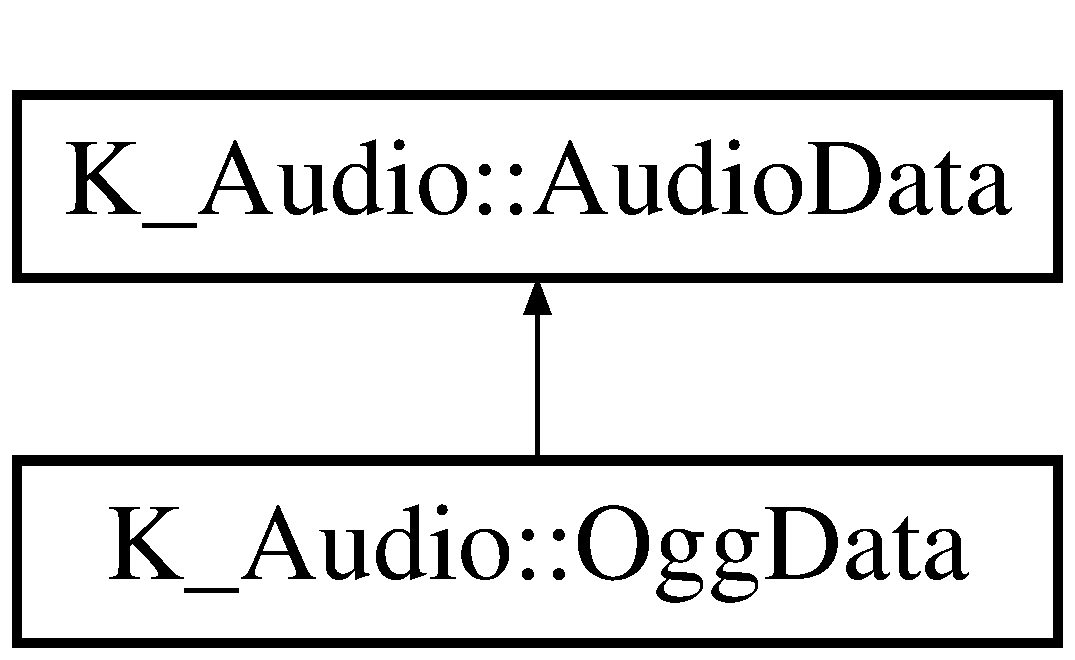
\includegraphics[height=2.000000cm]{class_k___audio_1_1_ogg_data}
\end{center}
\end{figure}
\subsection*{公開メンバ関数}
\begin{DoxyCompactItemize}
\item 
\mbox{\hyperlink{class_k___audio_1_1_ogg_data_a846e59bd024858fee33549b66f2697eb}{Ogg\+Data}} (const char $\ast$file\+Pass)
\item 
\mbox{\hyperlink{class_k___audio_1_1_ogg_data_a60aee716522004f16e11203677d3f63b}{$\sim$\+Ogg\+Data}} ()
\item 
void \mbox{\hyperlink{class_k___audio_1_1_ogg_data_aac0e955981398bf31053f27fbe19b2ba}{Seek}} (int offset)
\item 
int \mbox{\hyperlink{class_k___audio_1_1_ogg_data_ac4c50916e0f2eaa384539b2dbedc1d6e}{Read}} (char $\ast$buffer, int max\+Size)
\end{DoxyCompactItemize}
\subsection*{その他の継承メンバ}


\subsection{構築子と解体子}
\mbox{\Hypertarget{class_k___audio_1_1_ogg_data_a846e59bd024858fee33549b66f2697eb}\label{class_k___audio_1_1_ogg_data_a846e59bd024858fee33549b66f2697eb}} 
\index{K\+\_\+\+Audio\+::\+Ogg\+Data@{K\+\_\+\+Audio\+::\+Ogg\+Data}!Ogg\+Data@{Ogg\+Data}}
\index{Ogg\+Data@{Ogg\+Data}!K\+\_\+\+Audio\+::\+Ogg\+Data@{K\+\_\+\+Audio\+::\+Ogg\+Data}}
\subsubsection{\texorpdfstring{Ogg\+Data()}{OggData()}}
{\footnotesize\ttfamily K\+\_\+\+Audio\+::\+Ogg\+Data\+::\+Ogg\+Data (\begin{DoxyParamCaption}\item[{const char $\ast$}]{file\+Pass }\end{DoxyParamCaption})}

\mbox{\Hypertarget{class_k___audio_1_1_ogg_data_a60aee716522004f16e11203677d3f63b}\label{class_k___audio_1_1_ogg_data_a60aee716522004f16e11203677d3f63b}} 
\index{K\+\_\+\+Audio\+::\+Ogg\+Data@{K\+\_\+\+Audio\+::\+Ogg\+Data}!````~Ogg\+Data@{$\sim$\+Ogg\+Data}}
\index{````~Ogg\+Data@{$\sim$\+Ogg\+Data}!K\+\_\+\+Audio\+::\+Ogg\+Data@{K\+\_\+\+Audio\+::\+Ogg\+Data}}
\subsubsection{\texorpdfstring{$\sim$\+Ogg\+Data()}{~OggData()}}
{\footnotesize\ttfamily K\+\_\+\+Audio\+::\+Ogg\+Data\+::$\sim$\+Ogg\+Data (\begin{DoxyParamCaption}{ }\end{DoxyParamCaption})}



\subsection{関数詳解}
\mbox{\Hypertarget{class_k___audio_1_1_ogg_data_ac4c50916e0f2eaa384539b2dbedc1d6e}\label{class_k___audio_1_1_ogg_data_ac4c50916e0f2eaa384539b2dbedc1d6e}} 
\index{K\+\_\+\+Audio\+::\+Ogg\+Data@{K\+\_\+\+Audio\+::\+Ogg\+Data}!Read@{Read}}
\index{Read@{Read}!K\+\_\+\+Audio\+::\+Ogg\+Data@{K\+\_\+\+Audio\+::\+Ogg\+Data}}
\subsubsection{\texorpdfstring{Read()}{Read()}}
{\footnotesize\ttfamily int K\+\_\+\+Audio\+::\+Ogg\+Data\+::\+Read (\begin{DoxyParamCaption}\item[{char $\ast$}]{buffer,  }\item[{int}]{max\+Size }\end{DoxyParamCaption})\hspace{0.3cm}{\ttfamily [virtual]}}



\mbox{\hyperlink{class_k___audio_1_1_audio_data_af42b123ad2ce45867401d697fd572392}{K\+\_\+\+Audio\+::\+Audio\+Data}}を実装しています。

\mbox{\Hypertarget{class_k___audio_1_1_ogg_data_aac0e955981398bf31053f27fbe19b2ba}\label{class_k___audio_1_1_ogg_data_aac0e955981398bf31053f27fbe19b2ba}} 
\index{K\+\_\+\+Audio\+::\+Ogg\+Data@{K\+\_\+\+Audio\+::\+Ogg\+Data}!Seek@{Seek}}
\index{Seek@{Seek}!K\+\_\+\+Audio\+::\+Ogg\+Data@{K\+\_\+\+Audio\+::\+Ogg\+Data}}
\subsubsection{\texorpdfstring{Seek()}{Seek()}}
{\footnotesize\ttfamily void K\+\_\+\+Audio\+::\+Ogg\+Data\+::\+Seek (\begin{DoxyParamCaption}\item[{int}]{offset }\end{DoxyParamCaption})\hspace{0.3cm}{\ttfamily [virtual]}}



\mbox{\hyperlink{class_k___audio_1_1_audio_data_a1ba3ab1b4bae0b460d26278cb29ce16e}{K\+\_\+\+Audio\+::\+Audio\+Data}}を実装しています。


\hypertarget{struct_k___physics_1_1_map_polygon_1_1_polygon_data}{}\section{K\+\_\+\+Physics\+:\+:Map\+Polygon\+:\+:Polygon\+Data 構造体}
\label{struct_k___physics_1_1_map_polygon_1_1_polygon_data}\index{K\+\_\+\+Physics\+::\+Map\+Polygon\+::\+Polygon\+Data@{K\+\_\+\+Physics\+::\+Map\+Polygon\+::\+Polygon\+Data}}


{\ttfamily \#include $<$Map\+Polygon.\+h$>$}

\subsection*{公開変数類}
\begin{DoxyCompactItemize}
\item 
int \mbox{\hyperlink{struct_k___physics_1_1_map_polygon_1_1_polygon_data_a20746ae9989f097ffa21c9a0be396050}{num\+Polygon}}
\item 
\mbox{\hyperlink{struct_k___physics_1_1_map_polygon_1_1_polygon_type}{Polygon\+Type}} $\ast$ \mbox{\hyperlink{struct_k___physics_1_1_map_polygon_1_1_polygon_data_a510e830758a360dd1e0fd25c17f3b972}{polygon}}
\end{DoxyCompactItemize}


\subsection{メンバ詳解}
\mbox{\Hypertarget{struct_k___physics_1_1_map_polygon_1_1_polygon_data_a20746ae9989f097ffa21c9a0be396050}\label{struct_k___physics_1_1_map_polygon_1_1_polygon_data_a20746ae9989f097ffa21c9a0be396050}} 
\index{K\+\_\+\+Physics\+::\+Map\+Polygon\+::\+Polygon\+Data@{K\+\_\+\+Physics\+::\+Map\+Polygon\+::\+Polygon\+Data}!num\+Polygon@{num\+Polygon}}
\index{num\+Polygon@{num\+Polygon}!K\+\_\+\+Physics\+::\+Map\+Polygon\+::\+Polygon\+Data@{K\+\_\+\+Physics\+::\+Map\+Polygon\+::\+Polygon\+Data}}
\subsubsection{\texorpdfstring{num\+Polygon}{numPolygon}}
{\footnotesize\ttfamily int K\+\_\+\+Physics\+::\+Map\+Polygon\+::\+Polygon\+Data\+::num\+Polygon}

\mbox{\Hypertarget{struct_k___physics_1_1_map_polygon_1_1_polygon_data_a510e830758a360dd1e0fd25c17f3b972}\label{struct_k___physics_1_1_map_polygon_1_1_polygon_data_a510e830758a360dd1e0fd25c17f3b972}} 
\index{K\+\_\+\+Physics\+::\+Map\+Polygon\+::\+Polygon\+Data@{K\+\_\+\+Physics\+::\+Map\+Polygon\+::\+Polygon\+Data}!polygon@{polygon}}
\index{polygon@{polygon}!K\+\_\+\+Physics\+::\+Map\+Polygon\+::\+Polygon\+Data@{K\+\_\+\+Physics\+::\+Map\+Polygon\+::\+Polygon\+Data}}
\subsubsection{\texorpdfstring{polygon}{polygon}}
{\footnotesize\ttfamily \mbox{\hyperlink{struct_k___physics_1_1_map_polygon_1_1_polygon_type}{Polygon\+Type}}$\ast$ K\+\_\+\+Physics\+::\+Map\+Polygon\+::\+Polygon\+Data\+::polygon}


\hypertarget{struct_k___physics_1_1_map_polygon_1_1_polygon_type}{}\section{K\+\_\+\+Physics\+:\+:Map\+Polygon\+:\+:Polygon\+Type 構造体}
\label{struct_k___physics_1_1_map_polygon_1_1_polygon_type}\index{K\+\_\+\+Physics\+::\+Map\+Polygon\+::\+Polygon\+Type@{K\+\_\+\+Physics\+::\+Map\+Polygon\+::\+Polygon\+Type}}


{\ttfamily \#include $<$Map\+Polygon.\+h$>$}

\subsection*{公開変数類}
\begin{DoxyCompactItemize}
\item 
bt\+Vector3 \mbox{\hyperlink{struct_k___physics_1_1_map_polygon_1_1_polygon_type_a3288e14bc56fcea91db8359645fa496b}{point}} \mbox{[}3\mbox{]}
\end{DoxyCompactItemize}


\subsection{メンバ詳解}
\mbox{\Hypertarget{struct_k___physics_1_1_map_polygon_1_1_polygon_type_a3288e14bc56fcea91db8359645fa496b}\label{struct_k___physics_1_1_map_polygon_1_1_polygon_type_a3288e14bc56fcea91db8359645fa496b}} 
\index{K\+\_\+\+Physics\+::\+Map\+Polygon\+::\+Polygon\+Type@{K\+\_\+\+Physics\+::\+Map\+Polygon\+::\+Polygon\+Type}!point@{point}}
\index{point@{point}!K\+\_\+\+Physics\+::\+Map\+Polygon\+::\+Polygon\+Type@{K\+\_\+\+Physics\+::\+Map\+Polygon\+::\+Polygon\+Type}}
\subsubsection{\texorpdfstring{point}{point}}
{\footnotesize\ttfamily bt\+Vector3 K\+\_\+\+Physics\+::\+Map\+Polygon\+::\+Polygon\+Type\+::point\mbox{[}3\mbox{]}}


\hypertarget{class_k___graphics_1_1_shader_class}{}\section{K\+\_\+\+Graphics\+:\+:Shader\+Class クラス}
\label{class_k___graphics_1_1_shader_class}\index{K\+\_\+\+Graphics\+::\+Shader\+Class@{K\+\_\+\+Graphics\+::\+Shader\+Class}}


シェーダープログラムの管理とuniform変数の受け渡しを担当するクラス uniform変数名は固定的な機能を除くと、関数化にキリがないので汎用的な関数を用意  




{\ttfamily \#include $<$Shader\+Class.\+h$>$}

\subsection*{公開メンバ関数}
\begin{DoxyCompactItemize}
\item 
\mbox{\hyperlink{class_k___graphics_1_1_shader_class_a3762d1f3d62a5b9fe6b37d36aeb8dd51}{Shader\+Class}} (G\+Luint vertex\+Shader, G\+Luint fragment\+Shader)
\begin{DoxyCompactList}\small\item\em \mbox{\hyperlink{class_k___graphics_1_1_shader_class_ac37343a738ce216a5f1f3fb501de79ed}{Initialize()}}を呼ぶ \end{DoxyCompactList}\item 
\mbox{\hyperlink{class_k___graphics_1_1_shader_class_ad007e6356bf230f441fd39a5127b76d7}{$\sim$\+Shader\+Class}} ()
\begin{DoxyCompactList}\small\item\em \mbox{\hyperlink{class_k___graphics_1_1_shader_class_aac58eae7621bb220380364400f659549}{Finalize()}}を呼ぶ \end{DoxyCompactList}\item 
bool \mbox{\hyperlink{class_k___graphics_1_1_shader_class_ac37343a738ce216a5f1f3fb501de79ed}{Initialize}} (G\+Luint vertex\+Shader, G\+Luint fragment\+Shader)
\begin{DoxyCompactList}\small\item\em G\+L\+S\+Lシェーダープログラムを作成 \end{DoxyCompactList}\item 
void \mbox{\hyperlink{class_k___graphics_1_1_shader_class_aac58eae7621bb220380364400f659549}{Finalize}} ()
\begin{DoxyCompactList}\small\item\em シェーダーを開放する \end{DoxyCompactList}\item 
void \mbox{\hyperlink{class_k___graphics_1_1_shader_class_a53590f2a34bbf3f1dc91398068f43754}{Use\+Shader}} ()
\begin{DoxyCompactList}\small\item\em シェーダーを描画用に設定 \end{DoxyCompactList}\item 
void \mbox{\hyperlink{class_k___graphics_1_1_shader_class_a8aa0f7eb6c2443df15d483653f9401e3}{Set\+Matrix}} (const \mbox{\hyperlink{namespace_k___math_a345271af9d32dff2c964bc679b13b45c}{K\+\_\+\+Math\+::\+Matrix4x4}} \&mat)
\begin{DoxyCompactList}\small\item\em シェーダーに ワールド x ビュー x プロジェクション の行列を渡す \end{DoxyCompactList}\item 
void \mbox{\hyperlink{class_k___graphics_1_1_shader_class_ac697b99c625ac51a2dfeb01b85858506}{Set\+World\+Matrix}} (const \mbox{\hyperlink{namespace_k___math_a345271af9d32dff2c964bc679b13b45c}{K\+\_\+\+Math\+::\+Matrix4x4}} \&world)
\begin{DoxyCompactList}\small\item\em シェーダーにワールド行列だけを渡す \end{DoxyCompactList}\item 
void \mbox{\hyperlink{class_k___graphics_1_1_shader_class_a9d8fd3a0ab36010e685eecd735e6d296}{Set\+Texture}} (const std\+::string \&uniform\+Name, G\+Luint texture\+Layer, G\+Luint texture\+Number)
\begin{DoxyCompactList}\small\item\em シェーダーにテクスチャを渡す、モデル描画時に以下の番号が使われることがある レイヤー0番:モデルのマテリアルテクスチャ レイヤー1番:モデルのボーン行列テクスチャ \end{DoxyCompactList}\item 
void \mbox{\hyperlink{class_k___graphics_1_1_shader_class_a7a28da0b8fc149324d904150b711c397}{Set\+Directional\+Light}} (float power, const \mbox{\hyperlink{namespace_k___math_a8d82de9de17eae460600de1e40e8a01f}{K\+\_\+\+Math\+::\+Vector4}} \&color, const \mbox{\hyperlink{namespace_k___math_a66884d78082c39ada4091c211f3570f8}{K\+\_\+\+Math\+::\+Vector3}} \&direction)
\begin{DoxyCompactList}\small\item\em ディレクショナルライト情報を渡す \end{DoxyCompactList}\item 
void \mbox{\hyperlink{class_k___graphics_1_1_shader_class_acc9f55081fe01121e1010cd4754d5214}{Set\+Ambient\+Light}} (float power, const \mbox{\hyperlink{namespace_k___math_a8d82de9de17eae460600de1e40e8a01f}{K\+\_\+\+Math\+::\+Vector4}} \&color)
\begin{DoxyCompactList}\small\item\em アンビエントライト情報を渡す \end{DoxyCompactList}\item 
void \mbox{\hyperlink{class_k___graphics_1_1_shader_class_aa7151894bd962351e929e43f81490abe}{Set\+Value}} (const std\+::string \&uniform\+Name, int value)
\begin{DoxyCompactList}\small\item\em 汎用的なuniform変数への受け渡し \end{DoxyCompactList}\item 
void \mbox{\hyperlink{class_k___graphics_1_1_shader_class_a5cbcd8eca343a5e614edaf4def827ce1}{Set\+Value}} (const std\+::string \&uniform\+Name, float value)
\begin{DoxyCompactList}\small\item\em 汎用的なuniform変数への受け渡し \end{DoxyCompactList}\item 
void \mbox{\hyperlink{class_k___graphics_1_1_shader_class_a48af5c9168088ba35d222cb67f200a4e}{Set\+Value}} (const std\+::string \&uniform\+Name, const \mbox{\hyperlink{namespace_k___math_a345271af9d32dff2c964bc679b13b45c}{K\+\_\+\+Math\+::\+Matrix4x4}} \&value)
\begin{DoxyCompactList}\small\item\em 汎用的なuniform変数への受け渡し \end{DoxyCompactList}\item 
void \mbox{\hyperlink{class_k___graphics_1_1_shader_class_a90c6b0fa2ffc9016b442833b138b8a5a}{Set\+Value}} (const std\+::string \&uniform\+Name, const \mbox{\hyperlink{namespace_k___math_a8d82de9de17eae460600de1e40e8a01f}{K\+\_\+\+Math\+::\+Vector4}} \&value)
\begin{DoxyCompactList}\small\item\em 汎用的なuniform変数への受け渡し \end{DoxyCompactList}\item 
void \mbox{\hyperlink{class_k___graphics_1_1_shader_class_a0f81ce90173b0afe7dd98ea3c18f4913}{Set\+Value}} (const std\+::string \&uniform\+Name, const \mbox{\hyperlink{namespace_k___math_a66884d78082c39ada4091c211f3570f8}{K\+\_\+\+Math\+::\+Vector3}} \&value)
\begin{DoxyCompactList}\small\item\em 汎用的なuniform変数への受け渡し \end{DoxyCompactList}\item 
void \mbox{\hyperlink{class_k___graphics_1_1_shader_class_a37f4da2763c441b21cf9171268375d05}{Set\+Value}} (const std\+::string \&uniform\+Name, const \mbox{\hyperlink{namespace_k___math_a41eb0c2c69c938cd59989eb3241cefb2}{K\+\_\+\+Math\+::\+Vector2}} \&value)
\begin{DoxyCompactList}\small\item\em 汎用的なuniform変数への受け渡し \end{DoxyCompactList}\item 
void \mbox{\hyperlink{class_k___graphics_1_1_shader_class_a48edec1492bfa0fe8d8cab265c24bbbd}{Set\+Vertex\+Shader\+Subroutine}} (const std\+::string \&subroutine\+Function\+Name)
\begin{DoxyCompactList}\small\item\em subroutineの設定(vertex shader)、指定した名前の関数が選択される \end{DoxyCompactList}\item 
void \mbox{\hyperlink{class_k___graphics_1_1_shader_class_a8c25bbb391c95061db4d593679c96933}{Set\+Fragment\+Shader\+Subroutine}} (const std\+::string \&subroutine\+Function\+Name)
\begin{DoxyCompactList}\small\item\em subroutineの設定(fragment shader)、指定した名前の関数が選択される \end{DoxyCompactList}\end{DoxyCompactItemize}


\subsection{詳解}
シェーダープログラムの管理とuniform変数の受け渡しを担当するクラス uniform変数名は固定的な機能を除くと、関数化にキリがないので汎用的な関数を用意 

\subsection{構築子と解体子}
\mbox{\Hypertarget{class_k___graphics_1_1_shader_class_a3762d1f3d62a5b9fe6b37d36aeb8dd51}\label{class_k___graphics_1_1_shader_class_a3762d1f3d62a5b9fe6b37d36aeb8dd51}} 
\index{K\+\_\+\+Graphics\+::\+Shader\+Class@{K\+\_\+\+Graphics\+::\+Shader\+Class}!Shader\+Class@{Shader\+Class}}
\index{Shader\+Class@{Shader\+Class}!K\+\_\+\+Graphics\+::\+Shader\+Class@{K\+\_\+\+Graphics\+::\+Shader\+Class}}
\subsubsection{\texorpdfstring{Shader\+Class()}{ShaderClass()}}
{\footnotesize\ttfamily K\+\_\+\+Graphics\+::\+Shader\+Class\+::\+Shader\+Class (\begin{DoxyParamCaption}\item[{G\+Luint}]{vertex\+Shader,  }\item[{G\+Luint}]{fragment\+Shader }\end{DoxyParamCaption})}



\mbox{\hyperlink{class_k___graphics_1_1_shader_class_ac37343a738ce216a5f1f3fb501de79ed}{Initialize()}}を呼ぶ 

\mbox{\Hypertarget{class_k___graphics_1_1_shader_class_ad007e6356bf230f441fd39a5127b76d7}\label{class_k___graphics_1_1_shader_class_ad007e6356bf230f441fd39a5127b76d7}} 
\index{K\+\_\+\+Graphics\+::\+Shader\+Class@{K\+\_\+\+Graphics\+::\+Shader\+Class}!````~Shader\+Class@{$\sim$\+Shader\+Class}}
\index{````~Shader\+Class@{$\sim$\+Shader\+Class}!K\+\_\+\+Graphics\+::\+Shader\+Class@{K\+\_\+\+Graphics\+::\+Shader\+Class}}
\subsubsection{\texorpdfstring{$\sim$\+Shader\+Class()}{~ShaderClass()}}
{\footnotesize\ttfamily K\+\_\+\+Graphics\+::\+Shader\+Class\+::$\sim$\+Shader\+Class (\begin{DoxyParamCaption}{ }\end{DoxyParamCaption})}



\mbox{\hyperlink{class_k___graphics_1_1_shader_class_aac58eae7621bb220380364400f659549}{Finalize()}}を呼ぶ 



\subsection{関数詳解}
\mbox{\Hypertarget{class_k___graphics_1_1_shader_class_aac58eae7621bb220380364400f659549}\label{class_k___graphics_1_1_shader_class_aac58eae7621bb220380364400f659549}} 
\index{K\+\_\+\+Graphics\+::\+Shader\+Class@{K\+\_\+\+Graphics\+::\+Shader\+Class}!Finalize@{Finalize}}
\index{Finalize@{Finalize}!K\+\_\+\+Graphics\+::\+Shader\+Class@{K\+\_\+\+Graphics\+::\+Shader\+Class}}
\subsubsection{\texorpdfstring{Finalize()}{Finalize()}}
{\footnotesize\ttfamily void K\+\_\+\+Graphics\+::\+Shader\+Class\+::\+Finalize (\begin{DoxyParamCaption}{ }\end{DoxyParamCaption})}



シェーダーを開放する 

\mbox{\Hypertarget{class_k___graphics_1_1_shader_class_ac37343a738ce216a5f1f3fb501de79ed}\label{class_k___graphics_1_1_shader_class_ac37343a738ce216a5f1f3fb501de79ed}} 
\index{K\+\_\+\+Graphics\+::\+Shader\+Class@{K\+\_\+\+Graphics\+::\+Shader\+Class}!Initialize@{Initialize}}
\index{Initialize@{Initialize}!K\+\_\+\+Graphics\+::\+Shader\+Class@{K\+\_\+\+Graphics\+::\+Shader\+Class}}
\subsubsection{\texorpdfstring{Initialize()}{Initialize()}}
{\footnotesize\ttfamily bool K\+\_\+\+Graphics\+::\+Shader\+Class\+::\+Initialize (\begin{DoxyParamCaption}\item[{G\+Luint}]{vertex\+Shader,  }\item[{G\+Luint}]{fragment\+Shader }\end{DoxyParamCaption})}



G\+L\+S\+Lシェーダープログラムを作成 


\begin{DoxyParams}[1]{引数}
\mbox{\tt in}  & {\em vertex\+Shader} & 頂点シェーダーのインデックス \\
\hline
\mbox{\tt in}  & {\em fragment\+Shader} & フラグメントシェーダーのインデックス \\
\hline
\end{DoxyParams}
\begin{DoxyReturn}{戻り値}
成功するとtrue 
\end{DoxyReturn}
\mbox{\Hypertarget{class_k___graphics_1_1_shader_class_acc9f55081fe01121e1010cd4754d5214}\label{class_k___graphics_1_1_shader_class_acc9f55081fe01121e1010cd4754d5214}} 
\index{K\+\_\+\+Graphics\+::\+Shader\+Class@{K\+\_\+\+Graphics\+::\+Shader\+Class}!Set\+Ambient\+Light@{Set\+Ambient\+Light}}
\index{Set\+Ambient\+Light@{Set\+Ambient\+Light}!K\+\_\+\+Graphics\+::\+Shader\+Class@{K\+\_\+\+Graphics\+::\+Shader\+Class}}
\subsubsection{\texorpdfstring{Set\+Ambient\+Light()}{SetAmbientLight()}}
{\footnotesize\ttfamily void K\+\_\+\+Graphics\+::\+Shader\+Class\+::\+Set\+Ambient\+Light (\begin{DoxyParamCaption}\item[{float}]{power,  }\item[{const \mbox{\hyperlink{namespace_k___math_a8d82de9de17eae460600de1e40e8a01f}{K\+\_\+\+Math\+::\+Vector4}} \&}]{color }\end{DoxyParamCaption})}



アンビエントライト情報を渡す 


\begin{DoxyParams}[1]{引数}
\mbox{\tt in}  & {\em power} & 光の強さ \\
\hline
\mbox{\tt in}  & {\em color} & 光の色 \\
\hline
\end{DoxyParams}
\mbox{\Hypertarget{class_k___graphics_1_1_shader_class_a7a28da0b8fc149324d904150b711c397}\label{class_k___graphics_1_1_shader_class_a7a28da0b8fc149324d904150b711c397}} 
\index{K\+\_\+\+Graphics\+::\+Shader\+Class@{K\+\_\+\+Graphics\+::\+Shader\+Class}!Set\+Directional\+Light@{Set\+Directional\+Light}}
\index{Set\+Directional\+Light@{Set\+Directional\+Light}!K\+\_\+\+Graphics\+::\+Shader\+Class@{K\+\_\+\+Graphics\+::\+Shader\+Class}}
\subsubsection{\texorpdfstring{Set\+Directional\+Light()}{SetDirectionalLight()}}
{\footnotesize\ttfamily void K\+\_\+\+Graphics\+::\+Shader\+Class\+::\+Set\+Directional\+Light (\begin{DoxyParamCaption}\item[{float}]{power,  }\item[{const \mbox{\hyperlink{namespace_k___math_a8d82de9de17eae460600de1e40e8a01f}{K\+\_\+\+Math\+::\+Vector4}} \&}]{color,  }\item[{const \mbox{\hyperlink{namespace_k___math_a66884d78082c39ada4091c211f3570f8}{K\+\_\+\+Math\+::\+Vector3}} \&}]{direction }\end{DoxyParamCaption})}



ディレクショナルライト情報を渡す 


\begin{DoxyParams}[1]{引数}
\mbox{\tt in}  & {\em power} & 光の強さ \\
\hline
\mbox{\tt in}  & {\em color} & 光の色 \\
\hline
\mbox{\tt in}  & {\em direction} & 光の向き \\
\hline
\end{DoxyParams}
\mbox{\Hypertarget{class_k___graphics_1_1_shader_class_a8c25bbb391c95061db4d593679c96933}\label{class_k___graphics_1_1_shader_class_a8c25bbb391c95061db4d593679c96933}} 
\index{K\+\_\+\+Graphics\+::\+Shader\+Class@{K\+\_\+\+Graphics\+::\+Shader\+Class}!Set\+Fragment\+Shader\+Subroutine@{Set\+Fragment\+Shader\+Subroutine}}
\index{Set\+Fragment\+Shader\+Subroutine@{Set\+Fragment\+Shader\+Subroutine}!K\+\_\+\+Graphics\+::\+Shader\+Class@{K\+\_\+\+Graphics\+::\+Shader\+Class}}
\subsubsection{\texorpdfstring{Set\+Fragment\+Shader\+Subroutine()}{SetFragmentShaderSubroutine()}}
{\footnotesize\ttfamily void K\+\_\+\+Graphics\+::\+Shader\+Class\+::\+Set\+Fragment\+Shader\+Subroutine (\begin{DoxyParamCaption}\item[{const std\+::string \&}]{subroutine\+Function\+Name }\end{DoxyParamCaption})}



subroutineの設定(fragment shader)、指定した名前の関数が選択される 


\begin{DoxyParams}{引数}
{\em subroutine\+Function\+Name} & 使用するサブルーチン関数の名前 \\
\hline
\end{DoxyParams}
\mbox{\Hypertarget{class_k___graphics_1_1_shader_class_a8aa0f7eb6c2443df15d483653f9401e3}\label{class_k___graphics_1_1_shader_class_a8aa0f7eb6c2443df15d483653f9401e3}} 
\index{K\+\_\+\+Graphics\+::\+Shader\+Class@{K\+\_\+\+Graphics\+::\+Shader\+Class}!Set\+Matrix@{Set\+Matrix}}
\index{Set\+Matrix@{Set\+Matrix}!K\+\_\+\+Graphics\+::\+Shader\+Class@{K\+\_\+\+Graphics\+::\+Shader\+Class}}
\subsubsection{\texorpdfstring{Set\+Matrix()}{SetMatrix()}}
{\footnotesize\ttfamily void K\+\_\+\+Graphics\+::\+Shader\+Class\+::\+Set\+Matrix (\begin{DoxyParamCaption}\item[{const \mbox{\hyperlink{namespace_k___math_a345271af9d32dff2c964bc679b13b45c}{K\+\_\+\+Math\+::\+Matrix4x4}} \&}]{mat }\end{DoxyParamCaption})}



シェーダーに ワールド x ビュー x プロジェクション の行列を渡す 


\begin{DoxyParams}[1]{引数}
\mbox{\tt in}  & {\em mat} & 渡す変換行列 \\
\hline
\end{DoxyParams}
\mbox{\Hypertarget{class_k___graphics_1_1_shader_class_a9d8fd3a0ab36010e685eecd735e6d296}\label{class_k___graphics_1_1_shader_class_a9d8fd3a0ab36010e685eecd735e6d296}} 
\index{K\+\_\+\+Graphics\+::\+Shader\+Class@{K\+\_\+\+Graphics\+::\+Shader\+Class}!Set\+Texture@{Set\+Texture}}
\index{Set\+Texture@{Set\+Texture}!K\+\_\+\+Graphics\+::\+Shader\+Class@{K\+\_\+\+Graphics\+::\+Shader\+Class}}
\subsubsection{\texorpdfstring{Set\+Texture()}{SetTexture()}}
{\footnotesize\ttfamily void K\+\_\+\+Graphics\+::\+Shader\+Class\+::\+Set\+Texture (\begin{DoxyParamCaption}\item[{const std\+::string \&}]{uniform\+Name,  }\item[{G\+Luint}]{texture\+Layer,  }\item[{G\+Luint}]{texture\+Number }\end{DoxyParamCaption})}



シェーダーにテクスチャを渡す、モデル描画時に以下の番号が使われることがある レイヤー0番:モデルのマテリアルテクスチャ レイヤー1番:モデルのボーン行列テクスチャ 


\begin{DoxyParams}[1]{引数}
\mbox{\tt in}  & {\em uniform\+Name} & G\+L\+S\+Lのテクスチャを指す\+Uniform変数の名前 \\
\hline
\mbox{\tt in}  & {\em texture\+Layer} & テクスチャのレイヤー、複数枚のテクスチャを渡すときは数字を変える \\
\hline
\mbox{\tt in}  & {\em texture\+Number} & テクスチャのインデックス \\
\hline
\end{DoxyParams}
\mbox{\Hypertarget{class_k___graphics_1_1_shader_class_aa7151894bd962351e929e43f81490abe}\label{class_k___graphics_1_1_shader_class_aa7151894bd962351e929e43f81490abe}} 
\index{K\+\_\+\+Graphics\+::\+Shader\+Class@{K\+\_\+\+Graphics\+::\+Shader\+Class}!Set\+Value@{Set\+Value}}
\index{Set\+Value@{Set\+Value}!K\+\_\+\+Graphics\+::\+Shader\+Class@{K\+\_\+\+Graphics\+::\+Shader\+Class}}
\subsubsection{\texorpdfstring{Set\+Value()}{SetValue()}\hspace{0.1cm}{\footnotesize\ttfamily [1/6]}}
{\footnotesize\ttfamily void K\+\_\+\+Graphics\+::\+Shader\+Class\+::\+Set\+Value (\begin{DoxyParamCaption}\item[{const std\+::string \&}]{uniform\+Name,  }\item[{int}]{value }\end{DoxyParamCaption})}



汎用的なuniform変数への受け渡し 


\begin{DoxyParams}[1]{引数}
\mbox{\tt in}  & {\em uniform\+Name} & G\+L\+S\+Lのテクスチャを指す\+Uniform変数の名前 \\
\hline
\mbox{\tt in}  & {\em value} & 渡す値 \\
\hline
\end{DoxyParams}
\mbox{\Hypertarget{class_k___graphics_1_1_shader_class_a5cbcd8eca343a5e614edaf4def827ce1}\label{class_k___graphics_1_1_shader_class_a5cbcd8eca343a5e614edaf4def827ce1}} 
\index{K\+\_\+\+Graphics\+::\+Shader\+Class@{K\+\_\+\+Graphics\+::\+Shader\+Class}!Set\+Value@{Set\+Value}}
\index{Set\+Value@{Set\+Value}!K\+\_\+\+Graphics\+::\+Shader\+Class@{K\+\_\+\+Graphics\+::\+Shader\+Class}}
\subsubsection{\texorpdfstring{Set\+Value()}{SetValue()}\hspace{0.1cm}{\footnotesize\ttfamily [2/6]}}
{\footnotesize\ttfamily void K\+\_\+\+Graphics\+::\+Shader\+Class\+::\+Set\+Value (\begin{DoxyParamCaption}\item[{const std\+::string \&}]{uniform\+Name,  }\item[{float}]{value }\end{DoxyParamCaption})}



汎用的なuniform変数への受け渡し 


\begin{DoxyParams}[1]{引数}
\mbox{\tt in}  & {\em uniform\+Name} & G\+L\+S\+Lのテクスチャを指す\+Uniform変数の名前 \\
\hline
\mbox{\tt in}  & {\em value} & 渡す値 \\
\hline
\end{DoxyParams}
\mbox{\Hypertarget{class_k___graphics_1_1_shader_class_a48af5c9168088ba35d222cb67f200a4e}\label{class_k___graphics_1_1_shader_class_a48af5c9168088ba35d222cb67f200a4e}} 
\index{K\+\_\+\+Graphics\+::\+Shader\+Class@{K\+\_\+\+Graphics\+::\+Shader\+Class}!Set\+Value@{Set\+Value}}
\index{Set\+Value@{Set\+Value}!K\+\_\+\+Graphics\+::\+Shader\+Class@{K\+\_\+\+Graphics\+::\+Shader\+Class}}
\subsubsection{\texorpdfstring{Set\+Value()}{SetValue()}\hspace{0.1cm}{\footnotesize\ttfamily [3/6]}}
{\footnotesize\ttfamily void K\+\_\+\+Graphics\+::\+Shader\+Class\+::\+Set\+Value (\begin{DoxyParamCaption}\item[{const std\+::string \&}]{uniform\+Name,  }\item[{const \mbox{\hyperlink{namespace_k___math_a345271af9d32dff2c964bc679b13b45c}{K\+\_\+\+Math\+::\+Matrix4x4}} \&}]{value }\end{DoxyParamCaption})}



汎用的なuniform変数への受け渡し 


\begin{DoxyParams}[1]{引数}
\mbox{\tt in}  & {\em uniform\+Name} & G\+L\+S\+Lのテクスチャを指す\+Uniform変数の名前 \\
\hline
\mbox{\tt in}  & {\em value} & 渡す値 \\
\hline
\end{DoxyParams}
\mbox{\Hypertarget{class_k___graphics_1_1_shader_class_a90c6b0fa2ffc9016b442833b138b8a5a}\label{class_k___graphics_1_1_shader_class_a90c6b0fa2ffc9016b442833b138b8a5a}} 
\index{K\+\_\+\+Graphics\+::\+Shader\+Class@{K\+\_\+\+Graphics\+::\+Shader\+Class}!Set\+Value@{Set\+Value}}
\index{Set\+Value@{Set\+Value}!K\+\_\+\+Graphics\+::\+Shader\+Class@{K\+\_\+\+Graphics\+::\+Shader\+Class}}
\subsubsection{\texorpdfstring{Set\+Value()}{SetValue()}\hspace{0.1cm}{\footnotesize\ttfamily [4/6]}}
{\footnotesize\ttfamily void K\+\_\+\+Graphics\+::\+Shader\+Class\+::\+Set\+Value (\begin{DoxyParamCaption}\item[{const std\+::string \&}]{uniform\+Name,  }\item[{const \mbox{\hyperlink{namespace_k___math_a8d82de9de17eae460600de1e40e8a01f}{K\+\_\+\+Math\+::\+Vector4}} \&}]{value }\end{DoxyParamCaption})}



汎用的なuniform変数への受け渡し 


\begin{DoxyParams}[1]{引数}
\mbox{\tt in}  & {\em uniform\+Name} & G\+L\+S\+Lのテクスチャを指す\+Uniform変数の名前 \\
\hline
\mbox{\tt in}  & {\em value} & 渡す値 \\
\hline
\end{DoxyParams}
\mbox{\Hypertarget{class_k___graphics_1_1_shader_class_a0f81ce90173b0afe7dd98ea3c18f4913}\label{class_k___graphics_1_1_shader_class_a0f81ce90173b0afe7dd98ea3c18f4913}} 
\index{K\+\_\+\+Graphics\+::\+Shader\+Class@{K\+\_\+\+Graphics\+::\+Shader\+Class}!Set\+Value@{Set\+Value}}
\index{Set\+Value@{Set\+Value}!K\+\_\+\+Graphics\+::\+Shader\+Class@{K\+\_\+\+Graphics\+::\+Shader\+Class}}
\subsubsection{\texorpdfstring{Set\+Value()}{SetValue()}\hspace{0.1cm}{\footnotesize\ttfamily [5/6]}}
{\footnotesize\ttfamily void K\+\_\+\+Graphics\+::\+Shader\+Class\+::\+Set\+Value (\begin{DoxyParamCaption}\item[{const std\+::string \&}]{uniform\+Name,  }\item[{const \mbox{\hyperlink{namespace_k___math_a66884d78082c39ada4091c211f3570f8}{K\+\_\+\+Math\+::\+Vector3}} \&}]{value }\end{DoxyParamCaption})}



汎用的なuniform変数への受け渡し 


\begin{DoxyParams}[1]{引数}
\mbox{\tt in}  & {\em uniform\+Name} & G\+L\+S\+Lのテクスチャを指す\+Uniform変数の名前 \\
\hline
\mbox{\tt in}  & {\em value} & 渡す値 \\
\hline
\end{DoxyParams}
\mbox{\Hypertarget{class_k___graphics_1_1_shader_class_a37f4da2763c441b21cf9171268375d05}\label{class_k___graphics_1_1_shader_class_a37f4da2763c441b21cf9171268375d05}} 
\index{K\+\_\+\+Graphics\+::\+Shader\+Class@{K\+\_\+\+Graphics\+::\+Shader\+Class}!Set\+Value@{Set\+Value}}
\index{Set\+Value@{Set\+Value}!K\+\_\+\+Graphics\+::\+Shader\+Class@{K\+\_\+\+Graphics\+::\+Shader\+Class}}
\subsubsection{\texorpdfstring{Set\+Value()}{SetValue()}\hspace{0.1cm}{\footnotesize\ttfamily [6/6]}}
{\footnotesize\ttfamily void K\+\_\+\+Graphics\+::\+Shader\+Class\+::\+Set\+Value (\begin{DoxyParamCaption}\item[{const std\+::string \&}]{uniform\+Name,  }\item[{const \mbox{\hyperlink{namespace_k___math_a41eb0c2c69c938cd59989eb3241cefb2}{K\+\_\+\+Math\+::\+Vector2}} \&}]{value }\end{DoxyParamCaption})}



汎用的なuniform変数への受け渡し 


\begin{DoxyParams}[1]{引数}
\mbox{\tt in}  & {\em uniform\+Name} & G\+L\+S\+Lのテクスチャを指す\+Uniform変数の名前 \\
\hline
\mbox{\tt in}  & {\em value} & 渡す値 \\
\hline
\end{DoxyParams}
\mbox{\Hypertarget{class_k___graphics_1_1_shader_class_a48edec1492bfa0fe8d8cab265c24bbbd}\label{class_k___graphics_1_1_shader_class_a48edec1492bfa0fe8d8cab265c24bbbd}} 
\index{K\+\_\+\+Graphics\+::\+Shader\+Class@{K\+\_\+\+Graphics\+::\+Shader\+Class}!Set\+Vertex\+Shader\+Subroutine@{Set\+Vertex\+Shader\+Subroutine}}
\index{Set\+Vertex\+Shader\+Subroutine@{Set\+Vertex\+Shader\+Subroutine}!K\+\_\+\+Graphics\+::\+Shader\+Class@{K\+\_\+\+Graphics\+::\+Shader\+Class}}
\subsubsection{\texorpdfstring{Set\+Vertex\+Shader\+Subroutine()}{SetVertexShaderSubroutine()}}
{\footnotesize\ttfamily void K\+\_\+\+Graphics\+::\+Shader\+Class\+::\+Set\+Vertex\+Shader\+Subroutine (\begin{DoxyParamCaption}\item[{const std\+::string \&}]{subroutine\+Function\+Name }\end{DoxyParamCaption})}



subroutineの設定(vertex shader)、指定した名前の関数が選択される 


\begin{DoxyParams}{引数}
{\em subroutine\+Function\+Name} & 使用するサブルーチン関数の名前 \\
\hline
\end{DoxyParams}
\mbox{\Hypertarget{class_k___graphics_1_1_shader_class_ac697b99c625ac51a2dfeb01b85858506}\label{class_k___graphics_1_1_shader_class_ac697b99c625ac51a2dfeb01b85858506}} 
\index{K\+\_\+\+Graphics\+::\+Shader\+Class@{K\+\_\+\+Graphics\+::\+Shader\+Class}!Set\+World\+Matrix@{Set\+World\+Matrix}}
\index{Set\+World\+Matrix@{Set\+World\+Matrix}!K\+\_\+\+Graphics\+::\+Shader\+Class@{K\+\_\+\+Graphics\+::\+Shader\+Class}}
\subsubsection{\texorpdfstring{Set\+World\+Matrix()}{SetWorldMatrix()}}
{\footnotesize\ttfamily void K\+\_\+\+Graphics\+::\+Shader\+Class\+::\+Set\+World\+Matrix (\begin{DoxyParamCaption}\item[{const \mbox{\hyperlink{namespace_k___math_a345271af9d32dff2c964bc679b13b45c}{K\+\_\+\+Math\+::\+Matrix4x4}} \&}]{world }\end{DoxyParamCaption})}



シェーダーにワールド行列だけを渡す 


\begin{DoxyParams}[1]{引数}
\mbox{\tt in}  & {\em mat} & 渡す変換行列 \\
\hline
\end{DoxyParams}
\mbox{\Hypertarget{class_k___graphics_1_1_shader_class_a53590f2a34bbf3f1dc91398068f43754}\label{class_k___graphics_1_1_shader_class_a53590f2a34bbf3f1dc91398068f43754}} 
\index{K\+\_\+\+Graphics\+::\+Shader\+Class@{K\+\_\+\+Graphics\+::\+Shader\+Class}!Use\+Shader@{Use\+Shader}}
\index{Use\+Shader@{Use\+Shader}!K\+\_\+\+Graphics\+::\+Shader\+Class@{K\+\_\+\+Graphics\+::\+Shader\+Class}}
\subsubsection{\texorpdfstring{Use\+Shader()}{UseShader()}}
{\footnotesize\ttfamily void K\+\_\+\+Graphics\+::\+Shader\+Class\+::\+Use\+Shader (\begin{DoxyParamCaption}{ }\end{DoxyParamCaption})}



シェーダーを描画用に設定 


\hypertarget{class_k___graphics_1_1_shader_list}{}\section{K\+\_\+\+Graphics\+:\+:Shader\+List クラス}
\label{class_k___graphics_1_1_shader_list}\index{K\+\_\+\+Graphics\+::\+Shader\+List@{K\+\_\+\+Graphics\+::\+Shader\+List}}


シェーダークラスをリストとして持ち、解放責任をもつクラス  




{\ttfamily \#include $<$Shader\+List.\+h$>$}

\subsection*{公開メンバ関数}
\begin{DoxyCompactItemize}
\item 
\mbox{\hyperlink{class_k___graphics_1_1_shader_list_a93645f83598573fa2695489fcac10b6f}{Shader\+List}} ()
\begin{DoxyCompactList}\small\item\em \mbox{\hyperlink{class_k___graphics_1_1_shader_list_af5d3c07fdd3519e2c79792a462e26fc3}{Initialize()}}を呼ぶ \end{DoxyCompactList}\item 
\mbox{\hyperlink{class_k___graphics_1_1_shader_list_a77ff9ce6e8e54ca516fd5ac4281688f6}{$\sim$\+Shader\+List}} ()
\begin{DoxyCompactList}\small\item\em \mbox{\hyperlink{class_k___graphics_1_1_shader_list_af5d3c07fdd3519e2c79792a462e26fc3}{Initialize()}}を呼ぶ \end{DoxyCompactList}\item 
void \mbox{\hyperlink{class_k___graphics_1_1_shader_list_af5d3c07fdd3519e2c79792a462e26fc3}{Initialize}} ()
\begin{DoxyCompactList}\small\item\em リストのシェーダーを全て開放する \end{DoxyCompactList}\item 
\mbox{\hyperlink{class_k___graphics_1_1_shader_class}{Shader\+Class}} $\ast$ \mbox{\hyperlink{class_k___graphics_1_1_shader_list_a04083fe5c271e708da835e934cb57b6e}{Get\+Shader}} (const std\+::string \&shader\+Name)
\begin{DoxyCompactList}\small\item\em シェーダーへのポインタを取得 \end{DoxyCompactList}\item 
\mbox{\hyperlink{class_k___graphics_1_1_shader_class}{Shader\+Class}} $\ast$ \mbox{\hyperlink{class_k___graphics_1_1_shader_list_ad903d8c4daca2f2296434afd5694a4c5}{Use\+Shader}} (const std\+::string \&shader\+Name)
\begin{DoxyCompactList}\small\item\em シェーダーを描画用に設定し、そのシェーダーへのポインタを返す \end{DoxyCompactList}\item 
void \mbox{\hyperlink{class_k___graphics_1_1_shader_list_a5caa3b1fa44d6f4459e0471ead6c87e0}{Load\+Vertex\+Shader}} (const std\+::string \&file\+Name)
\begin{DoxyCompactList}\small\item\em 頂点シェーダーを読み込み、失敗するとstring型のエラーメッセージを例外で送出する \end{DoxyCompactList}\item 
void \mbox{\hyperlink{class_k___graphics_1_1_shader_list_a5daf641dfbc9472b9fb37126cfad27c7}{Load\+Fragment\+Shader}} (const std\+::string \&file\+Name)
\begin{DoxyCompactList}\small\item\em フラグメントシェーダーを読み込み、失敗するとstring型のエラーメッセージを例外で送出する \end{DoxyCompactList}\item 
void \mbox{\hyperlink{class_k___graphics_1_1_shader_list_ad59998f21d1830a48ce6a336813218aa}{Create\+Shader\+Program}} (const std\+::string \&shader\+Name, const std\+::string \&vertex\+Shader, const std\+::string \&fragment\+Shader)
\begin{DoxyCompactList}\small\item\em 頂点シェーダーとフラグメントシェーダーを組み合わせてシェーダーを作成 元となるシェーダーがない場合はstring型のエラーメッセージを例外で送出する \end{DoxyCompactList}\end{DoxyCompactItemize}


\subsection{詳解}
シェーダークラスをリストとして持ち、解放責任をもつクラス 

\subsection{構築子と解体子}
\mbox{\Hypertarget{class_k___graphics_1_1_shader_list_a93645f83598573fa2695489fcac10b6f}\label{class_k___graphics_1_1_shader_list_a93645f83598573fa2695489fcac10b6f}} 
\index{K\+\_\+\+Graphics\+::\+Shader\+List@{K\+\_\+\+Graphics\+::\+Shader\+List}!Shader\+List@{Shader\+List}}
\index{Shader\+List@{Shader\+List}!K\+\_\+\+Graphics\+::\+Shader\+List@{K\+\_\+\+Graphics\+::\+Shader\+List}}
\subsubsection{\texorpdfstring{Shader\+List()}{ShaderList()}}
{\footnotesize\ttfamily K\+\_\+\+Graphics\+::\+Shader\+List\+::\+Shader\+List (\begin{DoxyParamCaption}{ }\end{DoxyParamCaption})}



\mbox{\hyperlink{class_k___graphics_1_1_shader_list_af5d3c07fdd3519e2c79792a462e26fc3}{Initialize()}}を呼ぶ 

\mbox{\Hypertarget{class_k___graphics_1_1_shader_list_a77ff9ce6e8e54ca516fd5ac4281688f6}\label{class_k___graphics_1_1_shader_list_a77ff9ce6e8e54ca516fd5ac4281688f6}} 
\index{K\+\_\+\+Graphics\+::\+Shader\+List@{K\+\_\+\+Graphics\+::\+Shader\+List}!````~Shader\+List@{$\sim$\+Shader\+List}}
\index{````~Shader\+List@{$\sim$\+Shader\+List}!K\+\_\+\+Graphics\+::\+Shader\+List@{K\+\_\+\+Graphics\+::\+Shader\+List}}
\subsubsection{\texorpdfstring{$\sim$\+Shader\+List()}{~ShaderList()}}
{\footnotesize\ttfamily K\+\_\+\+Graphics\+::\+Shader\+List\+::$\sim$\+Shader\+List (\begin{DoxyParamCaption}{ }\end{DoxyParamCaption})}



\mbox{\hyperlink{class_k___graphics_1_1_shader_list_af5d3c07fdd3519e2c79792a462e26fc3}{Initialize()}}を呼ぶ 



\subsection{関数詳解}
\mbox{\Hypertarget{class_k___graphics_1_1_shader_list_ad59998f21d1830a48ce6a336813218aa}\label{class_k___graphics_1_1_shader_list_ad59998f21d1830a48ce6a336813218aa}} 
\index{K\+\_\+\+Graphics\+::\+Shader\+List@{K\+\_\+\+Graphics\+::\+Shader\+List}!Create\+Shader\+Program@{Create\+Shader\+Program}}
\index{Create\+Shader\+Program@{Create\+Shader\+Program}!K\+\_\+\+Graphics\+::\+Shader\+List@{K\+\_\+\+Graphics\+::\+Shader\+List}}
\subsubsection{\texorpdfstring{Create\+Shader\+Program()}{CreateShaderProgram()}}
{\footnotesize\ttfamily void K\+\_\+\+Graphics\+::\+Shader\+List\+::\+Create\+Shader\+Program (\begin{DoxyParamCaption}\item[{const std\+::string \&}]{shader\+Name,  }\item[{const std\+::string \&}]{vertex\+Shader,  }\item[{const std\+::string \&}]{fragment\+Shader }\end{DoxyParamCaption})}



頂点シェーダーとフラグメントシェーダーを組み合わせてシェーダーを作成 元となるシェーダーがない場合はstring型のエラーメッセージを例外で送出する 


\begin{DoxyParams}[1]{引数}
\mbox{\tt in}  & {\em shader\+Name} & 作成するシェーダーのユーザー定義名 \\
\hline
\mbox{\tt in}  & {\em vertex\+Shader} & 元となる頂点シェーダーへのパス(\+Load\+Vertex\+Shader()の時にパスでシェーダー名が登録されている) \\
\hline
\mbox{\tt in}  & {\em vertex\+Shader} & 元となるフラグメントシェーダーへのパス(\+Load\+Fragment\+Shader()の時にパスでシェーダー名が登録されている) \\
\hline
\end{DoxyParams}
\mbox{\Hypertarget{class_k___graphics_1_1_shader_list_a04083fe5c271e708da835e934cb57b6e}\label{class_k___graphics_1_1_shader_list_a04083fe5c271e708da835e934cb57b6e}} 
\index{K\+\_\+\+Graphics\+::\+Shader\+List@{K\+\_\+\+Graphics\+::\+Shader\+List}!Get\+Shader@{Get\+Shader}}
\index{Get\+Shader@{Get\+Shader}!K\+\_\+\+Graphics\+::\+Shader\+List@{K\+\_\+\+Graphics\+::\+Shader\+List}}
\subsubsection{\texorpdfstring{Get\+Shader()}{GetShader()}}
{\footnotesize\ttfamily \mbox{\hyperlink{class_k___graphics_1_1_shader_class}{Shader\+Class}} $\ast$ K\+\_\+\+Graphics\+::\+Shader\+List\+::\+Get\+Shader (\begin{DoxyParamCaption}\item[{const std\+::string \&}]{shader\+Name }\end{DoxyParamCaption})}



シェーダーへのポインタを取得 


\begin{DoxyParams}[1]{引数}
\mbox{\tt in}  & {\em shader\+Name} & シェーダーの名前 \\
\hline
\end{DoxyParams}
\begin{DoxyReturn}{戻り値}
名前に対応したシェーダー 
\end{DoxyReturn}
\mbox{\Hypertarget{class_k___graphics_1_1_shader_list_af5d3c07fdd3519e2c79792a462e26fc3}\label{class_k___graphics_1_1_shader_list_af5d3c07fdd3519e2c79792a462e26fc3}} 
\index{K\+\_\+\+Graphics\+::\+Shader\+List@{K\+\_\+\+Graphics\+::\+Shader\+List}!Initialize@{Initialize}}
\index{Initialize@{Initialize}!K\+\_\+\+Graphics\+::\+Shader\+List@{K\+\_\+\+Graphics\+::\+Shader\+List}}
\subsubsection{\texorpdfstring{Initialize()}{Initialize()}}
{\footnotesize\ttfamily void K\+\_\+\+Graphics\+::\+Shader\+List\+::\+Initialize (\begin{DoxyParamCaption}{ }\end{DoxyParamCaption})}



リストのシェーダーを全て開放する 

\mbox{\Hypertarget{class_k___graphics_1_1_shader_list_a5daf641dfbc9472b9fb37126cfad27c7}\label{class_k___graphics_1_1_shader_list_a5daf641dfbc9472b9fb37126cfad27c7}} 
\index{K\+\_\+\+Graphics\+::\+Shader\+List@{K\+\_\+\+Graphics\+::\+Shader\+List}!Load\+Fragment\+Shader@{Load\+Fragment\+Shader}}
\index{Load\+Fragment\+Shader@{Load\+Fragment\+Shader}!K\+\_\+\+Graphics\+::\+Shader\+List@{K\+\_\+\+Graphics\+::\+Shader\+List}}
\subsubsection{\texorpdfstring{Load\+Fragment\+Shader()}{LoadFragmentShader()}}
{\footnotesize\ttfamily void K\+\_\+\+Graphics\+::\+Shader\+List\+::\+Load\+Fragment\+Shader (\begin{DoxyParamCaption}\item[{const std\+::string \&}]{file\+Name }\end{DoxyParamCaption})}



フラグメントシェーダーを読み込み、失敗するとstring型のエラーメッセージを例外で送出する 


\begin{DoxyParams}[1]{引数}
\mbox{\tt in}  & {\em filename} & シェーダーのパス \\
\hline
\end{DoxyParams}
\mbox{\Hypertarget{class_k___graphics_1_1_shader_list_a5caa3b1fa44d6f4459e0471ead6c87e0}\label{class_k___graphics_1_1_shader_list_a5caa3b1fa44d6f4459e0471ead6c87e0}} 
\index{K\+\_\+\+Graphics\+::\+Shader\+List@{K\+\_\+\+Graphics\+::\+Shader\+List}!Load\+Vertex\+Shader@{Load\+Vertex\+Shader}}
\index{Load\+Vertex\+Shader@{Load\+Vertex\+Shader}!K\+\_\+\+Graphics\+::\+Shader\+List@{K\+\_\+\+Graphics\+::\+Shader\+List}}
\subsubsection{\texorpdfstring{Load\+Vertex\+Shader()}{LoadVertexShader()}}
{\footnotesize\ttfamily void K\+\_\+\+Graphics\+::\+Shader\+List\+::\+Load\+Vertex\+Shader (\begin{DoxyParamCaption}\item[{const std\+::string \&}]{file\+Name }\end{DoxyParamCaption})}



頂点シェーダーを読み込み、失敗するとstring型のエラーメッセージを例外で送出する 


\begin{DoxyParams}[1]{引数}
\mbox{\tt in}  & {\em file\+Name} & シェーダーのパス \\
\hline
\end{DoxyParams}
\mbox{\Hypertarget{class_k___graphics_1_1_shader_list_ad903d8c4daca2f2296434afd5694a4c5}\label{class_k___graphics_1_1_shader_list_ad903d8c4daca2f2296434afd5694a4c5}} 
\index{K\+\_\+\+Graphics\+::\+Shader\+List@{K\+\_\+\+Graphics\+::\+Shader\+List}!Use\+Shader@{Use\+Shader}}
\index{Use\+Shader@{Use\+Shader}!K\+\_\+\+Graphics\+::\+Shader\+List@{K\+\_\+\+Graphics\+::\+Shader\+List}}
\subsubsection{\texorpdfstring{Use\+Shader()}{UseShader()}}
{\footnotesize\ttfamily \mbox{\hyperlink{class_k___graphics_1_1_shader_class}{Shader\+Class}} $\ast$ K\+\_\+\+Graphics\+::\+Shader\+List\+::\+Use\+Shader (\begin{DoxyParamCaption}\item[{const std\+::string \&}]{shader\+Name }\end{DoxyParamCaption})}



シェーダーを描画用に設定し、そのシェーダーへのポインタを返す 


\begin{DoxyParams}[1]{引数}
\mbox{\tt in}  & {\em shader\+Name} & シェーダーの名前 \\
\hline
\end{DoxyParams}
\begin{DoxyReturn}{戻り値}
名前に対応したシェーダー 
\end{DoxyReturn}

\hypertarget{class_k___audio_1_1_sound_class}{}\section{K\+\_\+\+Audio\+:\+:Sound\+Class クラス}
\label{class_k___audio_1_1_sound_class}\index{K\+\_\+\+Audio\+::\+Sound\+Class@{K\+\_\+\+Audio\+::\+Sound\+Class}}


Open\+A\+Lをラッピングしたクラス  




{\ttfamily \#include $<$Sound\+Class.\+h$>$}

\subsection*{公開メンバ関数}
\begin{DoxyCompactItemize}
\item 
\mbox{\hyperlink{class_k___audio_1_1_sound_class_a9aba0743522979791ed9e6fe0d39c942}{Sound\+Class}} ()
\begin{DoxyCompactList}\small\item\em Open\+A\+Lの初期化 \end{DoxyCompactList}\item 
\mbox{\hyperlink{class_k___audio_1_1_sound_class_ae2fe8f23da3db03d0fd664fc9dbb0caa}{$\sim$\+Sound\+Class}} ()
\begin{DoxyCompactList}\small\item\em サウンドソースを全て破棄 \end{DoxyCompactList}\item 
bool \mbox{\hyperlink{class_k___audio_1_1_sound_class_a0f86040076fd10b6eddab46c78cc5009}{Create\+Source}} (const char $\ast$source\+Name, const char $\ast$file\+Pass, \mbox{\hyperlink{class_k___audio_1_1_sound_source_ad0e58f4cea821bc4087ed13830b06f69}{Sound\+Source\+::\+Load\+Mode}} mode)
\begin{DoxyCompactList}\small\item\em サウンドソース作成 \end{DoxyCompactList}\item 
void \mbox{\hyperlink{class_k___audio_1_1_sound_class_ab7f65f8816604bdc37cb6e30671b2494}{Delete\+Source}} (const char $\ast$source\+Name)
\begin{DoxyCompactList}\small\item\em サウンドソースを削除 \end{DoxyCompactList}\item 
\mbox{\hyperlink{class_k___audio_1_1_sound_source}{Sound\+Source}} $\ast$ \mbox{\hyperlink{class_k___audio_1_1_sound_class_ab40ecce29808c35b2f37b29e36cf981d}{Get\+Source}} (const char $\ast$source\+Name)
\end{DoxyCompactItemize}


\subsection{詳解}
Open\+A\+Lをラッピングしたクラス 

\subsection{構築子と解体子}
\mbox{\Hypertarget{class_k___audio_1_1_sound_class_a9aba0743522979791ed9e6fe0d39c942}\label{class_k___audio_1_1_sound_class_a9aba0743522979791ed9e6fe0d39c942}} 
\index{K\+\_\+\+Audio\+::\+Sound\+Class@{K\+\_\+\+Audio\+::\+Sound\+Class}!Sound\+Class@{Sound\+Class}}
\index{Sound\+Class@{Sound\+Class}!K\+\_\+\+Audio\+::\+Sound\+Class@{K\+\_\+\+Audio\+::\+Sound\+Class}}
\subsubsection{\texorpdfstring{Sound\+Class()}{SoundClass()}}
{\footnotesize\ttfamily K\+\_\+\+Audio\+::\+Sound\+Class\+::\+Sound\+Class (\begin{DoxyParamCaption}{ }\end{DoxyParamCaption})}



Open\+A\+Lの初期化 

\mbox{\Hypertarget{class_k___audio_1_1_sound_class_ae2fe8f23da3db03d0fd664fc9dbb0caa}\label{class_k___audio_1_1_sound_class_ae2fe8f23da3db03d0fd664fc9dbb0caa}} 
\index{K\+\_\+\+Audio\+::\+Sound\+Class@{K\+\_\+\+Audio\+::\+Sound\+Class}!````~Sound\+Class@{$\sim$\+Sound\+Class}}
\index{````~Sound\+Class@{$\sim$\+Sound\+Class}!K\+\_\+\+Audio\+::\+Sound\+Class@{K\+\_\+\+Audio\+::\+Sound\+Class}}
\subsubsection{\texorpdfstring{$\sim$\+Sound\+Class()}{~SoundClass()}}
{\footnotesize\ttfamily K\+\_\+\+Audio\+::\+Sound\+Class\+::$\sim$\+Sound\+Class (\begin{DoxyParamCaption}{ }\end{DoxyParamCaption})}



サウンドソースを全て破棄 



\subsection{関数詳解}
\mbox{\Hypertarget{class_k___audio_1_1_sound_class_a0f86040076fd10b6eddab46c78cc5009}\label{class_k___audio_1_1_sound_class_a0f86040076fd10b6eddab46c78cc5009}} 
\index{K\+\_\+\+Audio\+::\+Sound\+Class@{K\+\_\+\+Audio\+::\+Sound\+Class}!Create\+Source@{Create\+Source}}
\index{Create\+Source@{Create\+Source}!K\+\_\+\+Audio\+::\+Sound\+Class@{K\+\_\+\+Audio\+::\+Sound\+Class}}
\subsubsection{\texorpdfstring{Create\+Source()}{CreateSource()}}
{\footnotesize\ttfamily bool K\+\_\+\+Audio\+::\+Sound\+Class\+::\+Create\+Source (\begin{DoxyParamCaption}\item[{const char $\ast$}]{source\+Name,  }\item[{const char $\ast$}]{file\+Pass,  }\item[{\mbox{\hyperlink{class_k___audio_1_1_sound_source_ad0e58f4cea821bc4087ed13830b06f69}{Sound\+Source\+::\+Load\+Mode}}}]{mode }\end{DoxyParamCaption})}



サウンドソース作成 


\begin{DoxyParams}[1]{引数}
\mbox{\tt in}  & {\em source\+Name} & サウンドソースのユーザー定義名 \\
\hline
\mbox{\tt in}  & {\em file\+Pass} & サウンドのファイルパス(\+O\+GG と W\+A\+VE のみ) \\
\hline
\end{DoxyParams}
\begin{DoxyReturn}{戻り値}
成功するとtrue 
\end{DoxyReturn}
\mbox{\Hypertarget{class_k___audio_1_1_sound_class_ab7f65f8816604bdc37cb6e30671b2494}\label{class_k___audio_1_1_sound_class_ab7f65f8816604bdc37cb6e30671b2494}} 
\index{K\+\_\+\+Audio\+::\+Sound\+Class@{K\+\_\+\+Audio\+::\+Sound\+Class}!Delete\+Source@{Delete\+Source}}
\index{Delete\+Source@{Delete\+Source}!K\+\_\+\+Audio\+::\+Sound\+Class@{K\+\_\+\+Audio\+::\+Sound\+Class}}
\subsubsection{\texorpdfstring{Delete\+Source()}{DeleteSource()}}
{\footnotesize\ttfamily void K\+\_\+\+Audio\+::\+Sound\+Class\+::\+Delete\+Source (\begin{DoxyParamCaption}\item[{const char $\ast$}]{source\+Name }\end{DoxyParamCaption})}



サウンドソースを削除 


\begin{DoxyParams}[1]{引数}
\mbox{\tt in}  & {\em 削除するサウンドソースの名前} & \\
\hline
\end{DoxyParams}
\mbox{\Hypertarget{class_k___audio_1_1_sound_class_ab40ecce29808c35b2f37b29e36cf981d}\label{class_k___audio_1_1_sound_class_ab40ecce29808c35b2f37b29e36cf981d}} 
\index{K\+\_\+\+Audio\+::\+Sound\+Class@{K\+\_\+\+Audio\+::\+Sound\+Class}!Get\+Source@{Get\+Source}}
\index{Get\+Source@{Get\+Source}!K\+\_\+\+Audio\+::\+Sound\+Class@{K\+\_\+\+Audio\+::\+Sound\+Class}}
\subsubsection{\texorpdfstring{Get\+Source()}{GetSource()}}
{\footnotesize\ttfamily \mbox{\hyperlink{class_k___audio_1_1_sound_source}{Sound\+Source}}$\ast$ K\+\_\+\+Audio\+::\+Sound\+Class\+::\+Get\+Source (\begin{DoxyParamCaption}\item[{const char $\ast$}]{source\+Name }\end{DoxyParamCaption})}


\begin{DoxyParams}[1]{引数}
\mbox{\tt in}  & {\em サウンドソースの名前} & \\
\hline
\end{DoxyParams}
\begin{DoxyReturn}{戻り値}
サウンドソースへのポインタ 
\end{DoxyReturn}

\hypertarget{class_k___audio_1_1_sound_source}{}\section{K\+\_\+\+Audio\+:\+:Sound\+Source クラス}
\label{class_k___audio_1_1_sound_source}\index{K\+\_\+\+Audio\+::\+Sound\+Source@{K\+\_\+\+Audio\+::\+Sound\+Source}}


音源クラス~\newline
ループフラグが下りているときはファイル終端に到達した時点でストリーミングを終える  




{\ttfamily \#include $<$Sound\+Source.\+h$>$}

\subsection*{公開型}
\begin{DoxyCompactItemize}
\item 
enum \mbox{\hyperlink{class_k___audio_1_1_sound_source_ad0e58f4cea821bc4087ed13830b06f69}{Load\+Mode}} \{ \mbox{\hyperlink{class_k___audio_1_1_sound_source_ad0e58f4cea821bc4087ed13830b06f69a93ac3d22ea295b4cee4a699c6710402e}{Streaming}}, 
\mbox{\hyperlink{class_k___audio_1_1_sound_source_ad0e58f4cea821bc4087ed13830b06f69a510c98197d74c0c8ea23a66a1c8a3e53}{All\+Read}}
 \}
\begin{DoxyCompactList}\small\item\em 「全て読み込む」「ストリーミング再生」の二つを持つ \end{DoxyCompactList}\end{DoxyCompactItemize}
\subsection*{公開メンバ関数}
\begin{DoxyCompactItemize}
\item 
\mbox{\hyperlink{class_k___audio_1_1_sound_source_adcc7a2e8a6ba4203b9c2ff94649e06d9}{Sound\+Source}} (const char $\ast$source\+Name, const char $\ast$file\+Pass, \mbox{\hyperlink{class_k___audio_1_1_sound_source_ad0e58f4cea821bc4087ed13830b06f69}{Load\+Mode}} mode, int num\+Buffer=32)
\begin{DoxyCompactList}\small\item\em 情報を初期化 \end{DoxyCompactList}\item 
\mbox{\hyperlink{class_k___audio_1_1_sound_source_afe318e8ffc35a8774c36c2dfe7a05546}{$\sim$\+Sound\+Source}} ()
\begin{DoxyCompactList}\small\item\em 音声ファイルのポインタをdeleteする \end{DoxyCompactList}\item 
void \mbox{\hyperlink{class_k___audio_1_1_sound_source_a6d7aca76e2324325dc5f90b1ad3ce8b6}{Play}} (bool loop)
\begin{DoxyCompactList}\small\item\em 音声を再生 \end{DoxyCompactList}\item 
void \mbox{\hyperlink{class_k___audio_1_1_sound_source_ad9647ee76e3d5ae4f7c43f0bdcff2b77}{Play\+Copy}} ()
\begin{DoxyCompactList}\small\item\em 音声をコピーして再生(\+Load\+Modeが\+All\+Read時のみ使え、連続再生時音が重なる) \end{DoxyCompactList}\item 
void \mbox{\hyperlink{class_k___audio_1_1_sound_source_a47974ac6ed248793c8f2385618eb9cc0}{Pause}} ()
\begin{DoxyCompactList}\small\item\em 音声を一時停止 \end{DoxyCompactList}\item 
void \mbox{\hyperlink{class_k___audio_1_1_sound_source_a0c666b4b7b12c5e4412fb519d3786526}{Stop}} ()
\begin{DoxyCompactList}\small\item\em 音声を停止 \end{DoxyCompactList}\item 
void \mbox{\hyperlink{class_k___audio_1_1_sound_source_a7cae6d62c0635bc94bf8a2afccc32b9a}{Set\+Volume}} (float volume)
\begin{DoxyCompactList}\small\item\em 音声のボリュームを設定(0.0fが最低で、1.0fが最大) \end{DoxyCompactList}\item 
void \mbox{\hyperlink{class_k___audio_1_1_sound_source_a318fd679d40894f4568e6e9a50ff023f}{Set\+Position}} (float x, float y, float z)
\begin{DoxyCompactList}\small\item\em 音声の位置を設定 \end{DoxyCompactList}\item 
void \mbox{\hyperlink{class_k___audio_1_1_sound_source_a04c7824dd29a005186d66d1e1bd7cf4c}{Set\+Velocity}} (float x, float y, float z)
\begin{DoxyCompactList}\small\item\em 音声の移動速度を設定(ドップラー効果を得られる) \end{DoxyCompactList}\item 
bool \mbox{\hyperlink{class_k___audio_1_1_sound_source_a81fee1252efe87d2003433d30312cb3c}{Is\+Play}} ()
\end{DoxyCompactItemize}


\subsection{詳解}
音源クラス~\newline
ループフラグが下りているときはファイル終端に到達した時点でストリーミングを終える 

\subsection{列挙型メンバ詳解}
\mbox{\Hypertarget{class_k___audio_1_1_sound_source_ad0e58f4cea821bc4087ed13830b06f69}\label{class_k___audio_1_1_sound_source_ad0e58f4cea821bc4087ed13830b06f69}} 
\index{K\+\_\+\+Audio\+::\+Sound\+Source@{K\+\_\+\+Audio\+::\+Sound\+Source}!Load\+Mode@{Load\+Mode}}
\index{Load\+Mode@{Load\+Mode}!K\+\_\+\+Audio\+::\+Sound\+Source@{K\+\_\+\+Audio\+::\+Sound\+Source}}
\subsubsection{\texorpdfstring{Load\+Mode}{LoadMode}}
{\footnotesize\ttfamily enum \mbox{\hyperlink{class_k___audio_1_1_sound_source_ad0e58f4cea821bc4087ed13830b06f69}{K\+\_\+\+Audio\+::\+Sound\+Source\+::\+Load\+Mode}}}



「全て読み込む」「ストリーミング再生」の二つを持つ 

\begin{DoxyEnumFields}{列挙値}
\raisebox{\heightof{T}}[0pt][0pt]{\index{Streaming@{Streaming}!K\+\_\+\+Audio\+::\+Sound\+Source@{K\+\_\+\+Audio\+::\+Sound\+Source}}\index{K\+\_\+\+Audio\+::\+Sound\+Source@{K\+\_\+\+Audio\+::\+Sound\+Source}!Streaming@{Streaming}}}\mbox{\Hypertarget{class_k___audio_1_1_sound_source_ad0e58f4cea821bc4087ed13830b06f69a93ac3d22ea295b4cee4a699c6710402e}\label{class_k___audio_1_1_sound_source_ad0e58f4cea821bc4087ed13830b06f69a93ac3d22ea295b4cee4a699c6710402e}} 
Streaming&\\
\hline

\raisebox{\heightof{T}}[0pt][0pt]{\index{All\+Read@{All\+Read}!K\+\_\+\+Audio\+::\+Sound\+Source@{K\+\_\+\+Audio\+::\+Sound\+Source}}\index{K\+\_\+\+Audio\+::\+Sound\+Source@{K\+\_\+\+Audio\+::\+Sound\+Source}!All\+Read@{All\+Read}}}\mbox{\Hypertarget{class_k___audio_1_1_sound_source_ad0e58f4cea821bc4087ed13830b06f69a510c98197d74c0c8ea23a66a1c8a3e53}\label{class_k___audio_1_1_sound_source_ad0e58f4cea821bc4087ed13830b06f69a510c98197d74c0c8ea23a66a1c8a3e53}} 
All\+Read&\\
\hline

\end{DoxyEnumFields}


\subsection{構築子と解体子}
\mbox{\Hypertarget{class_k___audio_1_1_sound_source_adcc7a2e8a6ba4203b9c2ff94649e06d9}\label{class_k___audio_1_1_sound_source_adcc7a2e8a6ba4203b9c2ff94649e06d9}} 
\index{K\+\_\+\+Audio\+::\+Sound\+Source@{K\+\_\+\+Audio\+::\+Sound\+Source}!Sound\+Source@{Sound\+Source}}
\index{Sound\+Source@{Sound\+Source}!K\+\_\+\+Audio\+::\+Sound\+Source@{K\+\_\+\+Audio\+::\+Sound\+Source}}
\subsubsection{\texorpdfstring{Sound\+Source()}{SoundSource()}}
{\footnotesize\ttfamily K\+\_\+\+Audio\+::\+Sound\+Source\+::\+Sound\+Source (\begin{DoxyParamCaption}\item[{const char $\ast$}]{source\+Name,  }\item[{const char $\ast$}]{file\+Pass,  }\item[{\mbox{\hyperlink{class_k___audio_1_1_sound_source_ad0e58f4cea821bc4087ed13830b06f69}{Load\+Mode}}}]{mode,  }\item[{int}]{num\+Buffer = {\ttfamily 32} }\end{DoxyParamCaption})}



情報を初期化 


\begin{DoxyParams}[1]{引数}
\mbox{\tt in}  & {\em source\+Name} & このソースのユーザー定義名 \\
\hline
\mbox{\tt in}  & {\em file\+Pass} & 音声ファイルのパス \\
\hline
\mbox{\tt in}  & {\em mode} & 読み込みモード(\+Play\+Copy()は\+All\+Readモードの時にのみ使用可能) \\
\hline
\mbox{\tt in}  & {\em num\+Buffer} & ストリーミング再生時のバッファの数(省略時32個) \\
\hline
\end{DoxyParams}
\mbox{\Hypertarget{class_k___audio_1_1_sound_source_afe318e8ffc35a8774c36c2dfe7a05546}\label{class_k___audio_1_1_sound_source_afe318e8ffc35a8774c36c2dfe7a05546}} 
\index{K\+\_\+\+Audio\+::\+Sound\+Source@{K\+\_\+\+Audio\+::\+Sound\+Source}!````~Sound\+Source@{$\sim$\+Sound\+Source}}
\index{````~Sound\+Source@{$\sim$\+Sound\+Source}!K\+\_\+\+Audio\+::\+Sound\+Source@{K\+\_\+\+Audio\+::\+Sound\+Source}}
\subsubsection{\texorpdfstring{$\sim$\+Sound\+Source()}{~SoundSource()}}
{\footnotesize\ttfamily K\+\_\+\+Audio\+::\+Sound\+Source\+::$\sim$\+Sound\+Source (\begin{DoxyParamCaption}{ }\end{DoxyParamCaption})}



音声ファイルのポインタをdeleteする 



\subsection{関数詳解}
\mbox{\Hypertarget{class_k___audio_1_1_sound_source_a81fee1252efe87d2003433d30312cb3c}\label{class_k___audio_1_1_sound_source_a81fee1252efe87d2003433d30312cb3c}} 
\index{K\+\_\+\+Audio\+::\+Sound\+Source@{K\+\_\+\+Audio\+::\+Sound\+Source}!Is\+Play@{Is\+Play}}
\index{Is\+Play@{Is\+Play}!K\+\_\+\+Audio\+::\+Sound\+Source@{K\+\_\+\+Audio\+::\+Sound\+Source}}
\subsubsection{\texorpdfstring{Is\+Play()}{IsPlay()}}
{\footnotesize\ttfamily bool K\+\_\+\+Audio\+::\+Sound\+Source\+::\+Is\+Play (\begin{DoxyParamCaption}{ }\end{DoxyParamCaption})}

\begin{DoxyReturn}{戻り値}
音声が再生中か 
\end{DoxyReturn}
\mbox{\Hypertarget{class_k___audio_1_1_sound_source_a47974ac6ed248793c8f2385618eb9cc0}\label{class_k___audio_1_1_sound_source_a47974ac6ed248793c8f2385618eb9cc0}} 
\index{K\+\_\+\+Audio\+::\+Sound\+Source@{K\+\_\+\+Audio\+::\+Sound\+Source}!Pause@{Pause}}
\index{Pause@{Pause}!K\+\_\+\+Audio\+::\+Sound\+Source@{K\+\_\+\+Audio\+::\+Sound\+Source}}
\subsubsection{\texorpdfstring{Pause()}{Pause()}}
{\footnotesize\ttfamily void K\+\_\+\+Audio\+::\+Sound\+Source\+::\+Pause (\begin{DoxyParamCaption}{ }\end{DoxyParamCaption})}



音声を一時停止 

\mbox{\Hypertarget{class_k___audio_1_1_sound_source_a6d7aca76e2324325dc5f90b1ad3ce8b6}\label{class_k___audio_1_1_sound_source_a6d7aca76e2324325dc5f90b1ad3ce8b6}} 
\index{K\+\_\+\+Audio\+::\+Sound\+Source@{K\+\_\+\+Audio\+::\+Sound\+Source}!Play@{Play}}
\index{Play@{Play}!K\+\_\+\+Audio\+::\+Sound\+Source@{K\+\_\+\+Audio\+::\+Sound\+Source}}
\subsubsection{\texorpdfstring{Play()}{Play()}}
{\footnotesize\ttfamily void K\+\_\+\+Audio\+::\+Sound\+Source\+::\+Play (\begin{DoxyParamCaption}\item[{bool}]{loop }\end{DoxyParamCaption})}



音声を再生 


\begin{DoxyParams}[1]{引数}
\mbox{\tt in}  & {\em loop} & trueの時に音声を繰り返し再生 \\
\hline
\end{DoxyParams}
\mbox{\Hypertarget{class_k___audio_1_1_sound_source_ad9647ee76e3d5ae4f7c43f0bdcff2b77}\label{class_k___audio_1_1_sound_source_ad9647ee76e3d5ae4f7c43f0bdcff2b77}} 
\index{K\+\_\+\+Audio\+::\+Sound\+Source@{K\+\_\+\+Audio\+::\+Sound\+Source}!Play\+Copy@{Play\+Copy}}
\index{Play\+Copy@{Play\+Copy}!K\+\_\+\+Audio\+::\+Sound\+Source@{K\+\_\+\+Audio\+::\+Sound\+Source}}
\subsubsection{\texorpdfstring{Play\+Copy()}{PlayCopy()}}
{\footnotesize\ttfamily void K\+\_\+\+Audio\+::\+Sound\+Source\+::\+Play\+Copy (\begin{DoxyParamCaption}{ }\end{DoxyParamCaption})}



音声をコピーして再生(\+Load\+Modeが\+All\+Read時のみ使え、連続再生時音が重なる) 

\mbox{\Hypertarget{class_k___audio_1_1_sound_source_a318fd679d40894f4568e6e9a50ff023f}\label{class_k___audio_1_1_sound_source_a318fd679d40894f4568e6e9a50ff023f}} 
\index{K\+\_\+\+Audio\+::\+Sound\+Source@{K\+\_\+\+Audio\+::\+Sound\+Source}!Set\+Position@{Set\+Position}}
\index{Set\+Position@{Set\+Position}!K\+\_\+\+Audio\+::\+Sound\+Source@{K\+\_\+\+Audio\+::\+Sound\+Source}}
\subsubsection{\texorpdfstring{Set\+Position()}{SetPosition()}}
{\footnotesize\ttfamily void K\+\_\+\+Audio\+::\+Sound\+Source\+::\+Set\+Position (\begin{DoxyParamCaption}\item[{float}]{x,  }\item[{float}]{y,  }\item[{float}]{z }\end{DoxyParamCaption})}



音声の位置を設定 


\begin{DoxyParams}[1]{引数}
\mbox{\tt in}  & {\em x} & 位置座標\+X軸 \\
\hline
\mbox{\tt in}  & {\em y} & 位置座標\+Y軸 \\
\hline
\mbox{\tt in}  & {\em z} & 位置座標\+Z軸 \\
\hline
\end{DoxyParams}
\mbox{\Hypertarget{class_k___audio_1_1_sound_source_a04c7824dd29a005186d66d1e1bd7cf4c}\label{class_k___audio_1_1_sound_source_a04c7824dd29a005186d66d1e1bd7cf4c}} 
\index{K\+\_\+\+Audio\+::\+Sound\+Source@{K\+\_\+\+Audio\+::\+Sound\+Source}!Set\+Velocity@{Set\+Velocity}}
\index{Set\+Velocity@{Set\+Velocity}!K\+\_\+\+Audio\+::\+Sound\+Source@{K\+\_\+\+Audio\+::\+Sound\+Source}}
\subsubsection{\texorpdfstring{Set\+Velocity()}{SetVelocity()}}
{\footnotesize\ttfamily void K\+\_\+\+Audio\+::\+Sound\+Source\+::\+Set\+Velocity (\begin{DoxyParamCaption}\item[{float}]{x,  }\item[{float}]{y,  }\item[{float}]{z }\end{DoxyParamCaption})}



音声の移動速度を設定(ドップラー効果を得られる) 


\begin{DoxyParams}[1]{引数}
\mbox{\tt in}  & {\em x} & 速度\+X成分 \\
\hline
\mbox{\tt in}  & {\em y} & 速度\+Y成分 \\
\hline
\mbox{\tt in}  & {\em z} & 速度\+Z成分 \\
\hline
\end{DoxyParams}
\mbox{\Hypertarget{class_k___audio_1_1_sound_source_a7cae6d62c0635bc94bf8a2afccc32b9a}\label{class_k___audio_1_1_sound_source_a7cae6d62c0635bc94bf8a2afccc32b9a}} 
\index{K\+\_\+\+Audio\+::\+Sound\+Source@{K\+\_\+\+Audio\+::\+Sound\+Source}!Set\+Volume@{Set\+Volume}}
\index{Set\+Volume@{Set\+Volume}!K\+\_\+\+Audio\+::\+Sound\+Source@{K\+\_\+\+Audio\+::\+Sound\+Source}}
\subsubsection{\texorpdfstring{Set\+Volume()}{SetVolume()}}
{\footnotesize\ttfamily void K\+\_\+\+Audio\+::\+Sound\+Source\+::\+Set\+Volume (\begin{DoxyParamCaption}\item[{float}]{volume }\end{DoxyParamCaption})}



音声のボリュームを設定(0.0fが最低で、1.0fが最大) 


\begin{DoxyParams}[1]{引数}
\mbox{\tt in}  & {\em volume} & 音量の値 \\
\hline
\end{DoxyParams}
\mbox{\Hypertarget{class_k___audio_1_1_sound_source_a0c666b4b7b12c5e4412fb519d3786526}\label{class_k___audio_1_1_sound_source_a0c666b4b7b12c5e4412fb519d3786526}} 
\index{K\+\_\+\+Audio\+::\+Sound\+Source@{K\+\_\+\+Audio\+::\+Sound\+Source}!Stop@{Stop}}
\index{Stop@{Stop}!K\+\_\+\+Audio\+::\+Sound\+Source@{K\+\_\+\+Audio\+::\+Sound\+Source}}
\subsubsection{\texorpdfstring{Stop()}{Stop()}}
{\footnotesize\ttfamily void K\+\_\+\+Audio\+::\+Sound\+Source\+::\+Stop (\begin{DoxyParamCaption}{ }\end{DoxyParamCaption})}



音声を停止 


\hypertarget{class_k___graphics_1_1_sprite_object}{}\section{K\+\_\+\+Graphics\+:\+:Sprite\+Object クラス}
\label{class_k___graphics_1_1_sprite_object}\index{K\+\_\+\+Graphics\+::\+Sprite\+Object@{K\+\_\+\+Graphics\+::\+Sprite\+Object}}


長さ1.0fの板ポリゴンの\+Model\+Classを内部で生成し、2\+D画像の描画に利用できる機能を付け加えたクラス  




{\ttfamily \#include $<$Mesh\+Model.\+h$>$}

\subsection*{公開メンバ関数}
\begin{DoxyCompactItemize}
\item 
\mbox{\hyperlink{class_k___graphics_1_1_sprite_object_a9fe538248d36f9b2c20688f0053af112}{Sprite\+Object}} (\mbox{\hyperlink{class_k___graphics_1_1_texture}{Texture}} $\ast$texture, float control\+PointX=0.\+0f, float control\+Point\+Y=0.\+0f)
\begin{DoxyCompactList}\small\item\em \mbox{\hyperlink{class_k___graphics_1_1_sprite_object_a7c0ebb444b7484f20c10ba657060d779}{Initialize()}}を呼ぶ \end{DoxyCompactList}\item 
\mbox{\hyperlink{class_k___graphics_1_1_sprite_object_a8df242841b57bc345eb790b1fd24dbb9}{$\sim$\+Sprite\+Object}} ()
\begin{DoxyCompactList}\small\item\em \mbox{\hyperlink{class_k___graphics_1_1_sprite_object_ab07a1bdede7da183545bd155193d9f80}{Finalize()}}を呼ぶ \end{DoxyCompactList}\item 
bool \mbox{\hyperlink{class_k___graphics_1_1_sprite_object_a7c0ebb444b7484f20c10ba657060d779}{Initialize}} (\mbox{\hyperlink{class_k___graphics_1_1_texture}{Texture}} $\ast$texture, float control\+PointX, float control\+PointY)
\begin{DoxyCompactList}\small\item\em 初期化、テクスチャを設定し、変形のコントロールポイント座標を指定することもできる \end{DoxyCompactList}\item 
void \mbox{\hyperlink{class_k___graphics_1_1_sprite_object_ab07a1bdede7da183545bd155193d9f80}{Finalize}} ()
\begin{DoxyCompactList}\small\item\em 終了処理 \end{DoxyCompactList}\item 
bool \mbox{\hyperlink{class_k___graphics_1_1_sprite_object_a0fa1e6994fc741d94c726c85e5f1ec99}{Set\+Texture}} (\mbox{\hyperlink{class_k___graphics_1_1_texture}{Texture}} $\ast$texture)
\begin{DoxyCompactList}\small\item\em 表示するテクスチャを変更する \end{DoxyCompactList}\item 
void \mbox{\hyperlink{class_k___graphics_1_1_sprite_object_a1d9eb5352fd073b17ea42b53786fa29a}{Draw2D}} (\mbox{\hyperlink{class_k___graphics_1_1_camera_class}{Camera\+Class}} $\ast$camera, \mbox{\hyperlink{class_k___graphics_1_1_shader_class}{Shader\+Class}} $\ast$shader, const \mbox{\hyperlink{struct_k___math_1_1_box2_d}{K\+\_\+\+Math\+::\+Box2D}} \&src, const \mbox{\hyperlink{struct_k___math_1_1_box2_d}{K\+\_\+\+Math\+::\+Box2D}} \&draw, float rotation)
\begin{DoxyCompactList}\small\item\em 2\+D描画を行う 「スクリーンのサイズをカメラに設定している」「平行投影のカメラである」「\+Z軸方向を向きと\+Z軸と平行」 という3つの条件を満たしたカメラを設定するとスクリーン座標での描画ができる \end{DoxyCompactList}\item 
void \mbox{\hyperlink{class_k___graphics_1_1_sprite_object_af288c290560faa26460fbff16a677439}{Draw3D}} (\mbox{\hyperlink{class_k___graphics_1_1_camera_class}{Camera\+Class}} $\ast$camera, \mbox{\hyperlink{class_k___graphics_1_1_shader_class}{Shader\+Class}} $\ast$shader, const \mbox{\hyperlink{struct_k___math_1_1_box2_d}{K\+\_\+\+Math\+::\+Box2D}} \&src, const \mbox{\hyperlink{namespace_k___math_a66884d78082c39ada4091c211f3570f8}{K\+\_\+\+Math\+::\+Vector3}} \&position, const \mbox{\hyperlink{namespace_k___math_a66884d78082c39ada4091c211f3570f8}{K\+\_\+\+Math\+::\+Vector3}} \&rotation, const \mbox{\hyperlink{namespace_k___math_a66884d78082c39ada4091c211f3570f8}{K\+\_\+\+Math\+::\+Vector3}} \&scale)
\begin{DoxyCompactList}\small\item\em 3\+D空間上に描画する、ただし必ずカメラの方を向くビルボードになる \end{DoxyCompactList}\end{DoxyCompactItemize}
\subsection*{公開変数類}
\begin{DoxyCompactItemize}
\item 
\mbox{\hyperlink{namespace_k___math_a41eb0c2c69c938cd59989eb3241cefb2}{K\+\_\+\+Math\+::\+Vector2}} \mbox{\hyperlink{class_k___graphics_1_1_sprite_object_ad5d76b9b0a30102d01abbb20bab285f8}{control\+Point}}
\begin{DoxyCompactList}\small\item\em コントロールポイントの座標 \end{DoxyCompactList}\end{DoxyCompactItemize}
\subsection*{限定公開メンバ関数}
\begin{DoxyCompactItemize}
\item 
void \mbox{\hyperlink{class_k___graphics_1_1_sprite_object_a4c731f8c8e7b35f4f2661a3d9d203f69}{Set\+Matrix}} (\mbox{\hyperlink{class_k___graphics_1_1_camera_class}{Camera\+Class}} $\ast$camera, \mbox{\hyperlink{class_k___graphics_1_1_shader_class}{Shader\+Class}} $\ast$shader, const \mbox{\hyperlink{namespace_k___math_a66884d78082c39ada4091c211f3570f8}{K\+\_\+\+Math\+::\+Vector3}} \&position, const \mbox{\hyperlink{namespace_k___math_a66884d78082c39ada4091c211f3570f8}{K\+\_\+\+Math\+::\+Vector3}} \&rotation, const \mbox{\hyperlink{namespace_k___math_a66884d78082c39ada4091c211f3570f8}{K\+\_\+\+Math\+::\+Vector3}} \&scale, bool bill\+Board)
\end{DoxyCompactItemize}
\subsection*{限定公開変数類}
\begin{DoxyCompactItemize}
\item 
\mbox{\hyperlink{class_k___graphics_1_1_mesh_model}{Mesh\+Model}} $\ast$ \mbox{\hyperlink{class_k___graphics_1_1_sprite_object_a91966c81a550dd6b04ccc0bd210c289d}{draw\+Model}}
\item 
\mbox{\hyperlink{class_k___graphics_1_1_texture}{Texture}} $\ast$ \mbox{\hyperlink{class_k___graphics_1_1_sprite_object_a7cf528d065c242528bf0bd407a139f09}{cullent\+Texture}}
\end{DoxyCompactItemize}


\subsection{詳解}
長さ1.0fの板ポリゴンの\+Model\+Classを内部で生成し、2\+D画像の描画に利用できる機能を付け加えたクラス 

\subsection{構築子と解体子}
\mbox{\Hypertarget{class_k___graphics_1_1_sprite_object_a9fe538248d36f9b2c20688f0053af112}\label{class_k___graphics_1_1_sprite_object_a9fe538248d36f9b2c20688f0053af112}} 
\index{K\+\_\+\+Graphics\+::\+Sprite\+Object@{K\+\_\+\+Graphics\+::\+Sprite\+Object}!Sprite\+Object@{Sprite\+Object}}
\index{Sprite\+Object@{Sprite\+Object}!K\+\_\+\+Graphics\+::\+Sprite\+Object@{K\+\_\+\+Graphics\+::\+Sprite\+Object}}
\subsubsection{\texorpdfstring{Sprite\+Object()}{SpriteObject()}}
{\footnotesize\ttfamily K\+\_\+\+Graphics\+::\+Sprite\+Object\+::\+Sprite\+Object (\begin{DoxyParamCaption}\item[{\mbox{\hyperlink{class_k___graphics_1_1_texture}{Texture}} $\ast$}]{texture,  }\item[{float}]{control\+PointX = {\ttfamily 0.0f},  }\item[{float}]{control\+PointY = {\ttfamily 0.0f} }\end{DoxyParamCaption})}



\mbox{\hyperlink{class_k___graphics_1_1_sprite_object_a7c0ebb444b7484f20c10ba657060d779}{Initialize()}}を呼ぶ 

\mbox{\Hypertarget{class_k___graphics_1_1_sprite_object_a8df242841b57bc345eb790b1fd24dbb9}\label{class_k___graphics_1_1_sprite_object_a8df242841b57bc345eb790b1fd24dbb9}} 
\index{K\+\_\+\+Graphics\+::\+Sprite\+Object@{K\+\_\+\+Graphics\+::\+Sprite\+Object}!````~Sprite\+Object@{$\sim$\+Sprite\+Object}}
\index{````~Sprite\+Object@{$\sim$\+Sprite\+Object}!K\+\_\+\+Graphics\+::\+Sprite\+Object@{K\+\_\+\+Graphics\+::\+Sprite\+Object}}
\subsubsection{\texorpdfstring{$\sim$\+Sprite\+Object()}{~SpriteObject()}}
{\footnotesize\ttfamily K\+\_\+\+Graphics\+::\+Sprite\+Object\+::$\sim$\+Sprite\+Object (\begin{DoxyParamCaption}{ }\end{DoxyParamCaption})}



\mbox{\hyperlink{class_k___graphics_1_1_sprite_object_ab07a1bdede7da183545bd155193d9f80}{Finalize()}}を呼ぶ 



\subsection{関数詳解}
\mbox{\Hypertarget{class_k___graphics_1_1_sprite_object_a1d9eb5352fd073b17ea42b53786fa29a}\label{class_k___graphics_1_1_sprite_object_a1d9eb5352fd073b17ea42b53786fa29a}} 
\index{K\+\_\+\+Graphics\+::\+Sprite\+Object@{K\+\_\+\+Graphics\+::\+Sprite\+Object}!Draw2D@{Draw2D}}
\index{Draw2D@{Draw2D}!K\+\_\+\+Graphics\+::\+Sprite\+Object@{K\+\_\+\+Graphics\+::\+Sprite\+Object}}
\subsubsection{\texorpdfstring{Draw2\+D()}{Draw2D()}}
{\footnotesize\ttfamily void K\+\_\+\+Graphics\+::\+Sprite\+Object\+::\+Draw2D (\begin{DoxyParamCaption}\item[{\mbox{\hyperlink{class_k___graphics_1_1_camera_class}{Camera\+Class}} $\ast$}]{camera,  }\item[{\mbox{\hyperlink{class_k___graphics_1_1_shader_class}{Shader\+Class}} $\ast$}]{shader,  }\item[{const \mbox{\hyperlink{struct_k___math_1_1_box2_d}{K\+\_\+\+Math\+::\+Box2D}} \&}]{src,  }\item[{const \mbox{\hyperlink{struct_k___math_1_1_box2_d}{K\+\_\+\+Math\+::\+Box2D}} \&}]{draw,  }\item[{float}]{rotation }\end{DoxyParamCaption})}



2\+D描画を行う 「スクリーンのサイズをカメラに設定している」「平行投影のカメラである」「\+Z軸方向を向きと\+Z軸と平行」 という3つの条件を満たしたカメラを設定するとスクリーン座標での描画ができる 


\begin{DoxyParams}[1]{引数}
\mbox{\tt in}  & {\em camera} & 使用するカメラ(上記の条件に注意) \\
\hline
\mbox{\tt in}  & {\em shader} & 使用するシェーダー \\
\hline
\mbox{\tt in}  & {\em src} & テクスチャの切り取り情報~\newline
「テクスチャのピクセル座標\+X\+Y」「矩形の幅と高さ」をそれぞれ\char`\"{}x\char`\"{}\char`\"{}y\char`\"{}\char`\"{}w\char`\"{}\char`\"{}h\char`\"{}に設定する \\
\hline
\mbox{\tt in}  & {\em draw} & 実際に描画する場所と大きさを指定する~\newline
「位置座標\+X\+Y」「矩形の幅と高さ」をそれぞれ\char`\"{}x\char`\"{}\char`\"{}y\char`\"{}\char`\"{}w\char`\"{}\char`\"{}h\char`\"{}に設定する \\
\hline
\mbox{\tt in}  & {\em rotation} & 右回転の角度(度数法) \\
\hline
\end{DoxyParams}
\mbox{\Hypertarget{class_k___graphics_1_1_sprite_object_af288c290560faa26460fbff16a677439}\label{class_k___graphics_1_1_sprite_object_af288c290560faa26460fbff16a677439}} 
\index{K\+\_\+\+Graphics\+::\+Sprite\+Object@{K\+\_\+\+Graphics\+::\+Sprite\+Object}!Draw3D@{Draw3D}}
\index{Draw3D@{Draw3D}!K\+\_\+\+Graphics\+::\+Sprite\+Object@{K\+\_\+\+Graphics\+::\+Sprite\+Object}}
\subsubsection{\texorpdfstring{Draw3\+D()}{Draw3D()}}
{\footnotesize\ttfamily void K\+\_\+\+Graphics\+::\+Sprite\+Object\+::\+Draw3D (\begin{DoxyParamCaption}\item[{\mbox{\hyperlink{class_k___graphics_1_1_camera_class}{Camera\+Class}} $\ast$}]{camera,  }\item[{\mbox{\hyperlink{class_k___graphics_1_1_shader_class}{Shader\+Class}} $\ast$}]{shader,  }\item[{const \mbox{\hyperlink{struct_k___math_1_1_box2_d}{K\+\_\+\+Math\+::\+Box2D}} \&}]{src,  }\item[{const \mbox{\hyperlink{namespace_k___math_a66884d78082c39ada4091c211f3570f8}{K\+\_\+\+Math\+::\+Vector3}} \&}]{position,  }\item[{const \mbox{\hyperlink{namespace_k___math_a66884d78082c39ada4091c211f3570f8}{K\+\_\+\+Math\+::\+Vector3}} \&}]{rotation,  }\item[{const \mbox{\hyperlink{namespace_k___math_a66884d78082c39ada4091c211f3570f8}{K\+\_\+\+Math\+::\+Vector3}} \&}]{scale }\end{DoxyParamCaption})}



3\+D空間上に描画する、ただし必ずカメラの方を向くビルボードになる 


\begin{DoxyParams}[1]{引数}
\mbox{\tt in}  & {\em camera} & 使用するカメラクラスへのポインタ \\
\hline
\mbox{\tt in}  & {\em shader} & 使用するシェーダーへのポインタ \\
\hline
\mbox{\tt in}  & {\em src} & テクスチャの切り取り情報~\newline
「テクスチャのピクセル座標\+X\+Y」「矩形の幅と高さ」をそれぞれ\char`\"{}x\char`\"{}\char`\"{}y\char`\"{}\char`\"{}w\char`\"{}\char`\"{}h\char`\"{}に設定する \\
\hline
\mbox{\tt in}  & {\em position} & 3\+D空間上の位置座標 \\
\hline
\mbox{\tt in}  & {\em rotation} & X\+Y\+Zそれぞれの軸に関する回転角度(度数法で\+Y→\+X→\+Zの順で回転する) \\
\hline
\mbox{\tt in}  & {\em scale} & スケーリング \\
\hline
\end{DoxyParams}
\mbox{\Hypertarget{class_k___graphics_1_1_sprite_object_ab07a1bdede7da183545bd155193d9f80}\label{class_k___graphics_1_1_sprite_object_ab07a1bdede7da183545bd155193d9f80}} 
\index{K\+\_\+\+Graphics\+::\+Sprite\+Object@{K\+\_\+\+Graphics\+::\+Sprite\+Object}!Finalize@{Finalize}}
\index{Finalize@{Finalize}!K\+\_\+\+Graphics\+::\+Sprite\+Object@{K\+\_\+\+Graphics\+::\+Sprite\+Object}}
\subsubsection{\texorpdfstring{Finalize()}{Finalize()}}
{\footnotesize\ttfamily void K\+\_\+\+Graphics\+::\+Sprite\+Object\+::\+Finalize (\begin{DoxyParamCaption}{ }\end{DoxyParamCaption})}



終了処理 

\mbox{\Hypertarget{class_k___graphics_1_1_sprite_object_a7c0ebb444b7484f20c10ba657060d779}\label{class_k___graphics_1_1_sprite_object_a7c0ebb444b7484f20c10ba657060d779}} 
\index{K\+\_\+\+Graphics\+::\+Sprite\+Object@{K\+\_\+\+Graphics\+::\+Sprite\+Object}!Initialize@{Initialize}}
\index{Initialize@{Initialize}!K\+\_\+\+Graphics\+::\+Sprite\+Object@{K\+\_\+\+Graphics\+::\+Sprite\+Object}}
\subsubsection{\texorpdfstring{Initialize()}{Initialize()}}
{\footnotesize\ttfamily bool K\+\_\+\+Graphics\+::\+Sprite\+Object\+::\+Initialize (\begin{DoxyParamCaption}\item[{\mbox{\hyperlink{class_k___graphics_1_1_texture}{Texture}} $\ast$}]{texture,  }\item[{float}]{control\+PointX,  }\item[{float}]{control\+PointY }\end{DoxyParamCaption})}



初期化、テクスチャを設定し、変形のコントロールポイント座標を指定することもできる 


\begin{DoxyParams}[1]{引数}
\mbox{\tt in}  & {\em texture} & 使用するテクスチャ、nullptrを指定することもできる \\
\hline
\mbox{\tt in}  & {\em control\+PointX} & コントロールポイント\+X座標~\newline
板ポリゴンを左上原点で変形の影響を受けない \\
\hline
\mbox{\tt in}  & {\em control\+PointY} & コントロールポイント\+Y座標~\newline
板ポリゴンを左上原点で変形の影響を受けない \\
\hline
\end{DoxyParams}
\mbox{\Hypertarget{class_k___graphics_1_1_sprite_object_a4c731f8c8e7b35f4f2661a3d9d203f69}\label{class_k___graphics_1_1_sprite_object_a4c731f8c8e7b35f4f2661a3d9d203f69}} 
\index{K\+\_\+\+Graphics\+::\+Sprite\+Object@{K\+\_\+\+Graphics\+::\+Sprite\+Object}!Set\+Matrix@{Set\+Matrix}}
\index{Set\+Matrix@{Set\+Matrix}!K\+\_\+\+Graphics\+::\+Sprite\+Object@{K\+\_\+\+Graphics\+::\+Sprite\+Object}}
\subsubsection{\texorpdfstring{Set\+Matrix()}{SetMatrix()}}
{\footnotesize\ttfamily void K\+\_\+\+Graphics\+::\+Sprite\+Object\+::\+Set\+Matrix (\begin{DoxyParamCaption}\item[{\mbox{\hyperlink{class_k___graphics_1_1_camera_class}{Camera\+Class}} $\ast$}]{camera,  }\item[{\mbox{\hyperlink{class_k___graphics_1_1_shader_class}{Shader\+Class}} $\ast$}]{shader,  }\item[{const \mbox{\hyperlink{namespace_k___math_a66884d78082c39ada4091c211f3570f8}{K\+\_\+\+Math\+::\+Vector3}} \&}]{position,  }\item[{const \mbox{\hyperlink{namespace_k___math_a66884d78082c39ada4091c211f3570f8}{K\+\_\+\+Math\+::\+Vector3}} \&}]{rotation,  }\item[{const \mbox{\hyperlink{namespace_k___math_a66884d78082c39ada4091c211f3570f8}{K\+\_\+\+Math\+::\+Vector3}} \&}]{scale,  }\item[{bool}]{bill\+Board }\end{DoxyParamCaption})\hspace{0.3cm}{\ttfamily [protected]}}

\mbox{\Hypertarget{class_k___graphics_1_1_sprite_object_a0fa1e6994fc741d94c726c85e5f1ec99}\label{class_k___graphics_1_1_sprite_object_a0fa1e6994fc741d94c726c85e5f1ec99}} 
\index{K\+\_\+\+Graphics\+::\+Sprite\+Object@{K\+\_\+\+Graphics\+::\+Sprite\+Object}!Set\+Texture@{Set\+Texture}}
\index{Set\+Texture@{Set\+Texture}!K\+\_\+\+Graphics\+::\+Sprite\+Object@{K\+\_\+\+Graphics\+::\+Sprite\+Object}}
\subsubsection{\texorpdfstring{Set\+Texture()}{SetTexture()}}
{\footnotesize\ttfamily bool K\+\_\+\+Graphics\+::\+Sprite\+Object\+::\+Set\+Texture (\begin{DoxyParamCaption}\item[{\mbox{\hyperlink{class_k___graphics_1_1_texture}{Texture}} $\ast$}]{texture }\end{DoxyParamCaption})}



表示するテクスチャを変更する 


\begin{DoxyParams}[1]{引数}
\mbox{\tt in}  & {\em texture} & 使用するテクスチャのポインタ \\
\hline
\end{DoxyParams}


\subsection{メンバ詳解}
\mbox{\Hypertarget{class_k___graphics_1_1_sprite_object_ad5d76b9b0a30102d01abbb20bab285f8}\label{class_k___graphics_1_1_sprite_object_ad5d76b9b0a30102d01abbb20bab285f8}} 
\index{K\+\_\+\+Graphics\+::\+Sprite\+Object@{K\+\_\+\+Graphics\+::\+Sprite\+Object}!control\+Point@{control\+Point}}
\index{control\+Point@{control\+Point}!K\+\_\+\+Graphics\+::\+Sprite\+Object@{K\+\_\+\+Graphics\+::\+Sprite\+Object}}
\subsubsection{\texorpdfstring{control\+Point}{controlPoint}}
{\footnotesize\ttfamily \mbox{\hyperlink{namespace_k___math_a41eb0c2c69c938cd59989eb3241cefb2}{K\+\_\+\+Math\+::\+Vector2}} K\+\_\+\+Graphics\+::\+Sprite\+Object\+::control\+Point}



コントロールポイントの座標 

\mbox{\Hypertarget{class_k___graphics_1_1_sprite_object_a7cf528d065c242528bf0bd407a139f09}\label{class_k___graphics_1_1_sprite_object_a7cf528d065c242528bf0bd407a139f09}} 
\index{K\+\_\+\+Graphics\+::\+Sprite\+Object@{K\+\_\+\+Graphics\+::\+Sprite\+Object}!cullent\+Texture@{cullent\+Texture}}
\index{cullent\+Texture@{cullent\+Texture}!K\+\_\+\+Graphics\+::\+Sprite\+Object@{K\+\_\+\+Graphics\+::\+Sprite\+Object}}
\subsubsection{\texorpdfstring{cullent\+Texture}{cullentTexture}}
{\footnotesize\ttfamily \mbox{\hyperlink{class_k___graphics_1_1_texture}{Texture}}$\ast$ K\+\_\+\+Graphics\+::\+Sprite\+Object\+::cullent\+Texture\hspace{0.3cm}{\ttfamily [protected]}}

\mbox{\Hypertarget{class_k___graphics_1_1_sprite_object_a91966c81a550dd6b04ccc0bd210c289d}\label{class_k___graphics_1_1_sprite_object_a91966c81a550dd6b04ccc0bd210c289d}} 
\index{K\+\_\+\+Graphics\+::\+Sprite\+Object@{K\+\_\+\+Graphics\+::\+Sprite\+Object}!draw\+Model@{draw\+Model}}
\index{draw\+Model@{draw\+Model}!K\+\_\+\+Graphics\+::\+Sprite\+Object@{K\+\_\+\+Graphics\+::\+Sprite\+Object}}
\subsubsection{\texorpdfstring{draw\+Model}{drawModel}}
{\footnotesize\ttfamily \mbox{\hyperlink{class_k___graphics_1_1_mesh_model}{Mesh\+Model}}$\ast$ K\+\_\+\+Graphics\+::\+Sprite\+Object\+::draw\+Model\hspace{0.3cm}{\ttfamily [protected]}}


\hypertarget{struct_k___input_1_1_stick_state}{}\section{K\+\_\+\+Input\+:\+:Stick\+State 構造体}
\label{struct_k___input_1_1_stick_state}\index{K\+\_\+\+Input\+::\+Stick\+State@{K\+\_\+\+Input\+::\+Stick\+State}}


横と縦の二軸を持つスティック  




{\ttfamily \#include $<$Vpad\+States.\+h$>$}

\subsection*{公開メンバ関数}
\begin{DoxyCompactItemize}
\item 
\mbox{\hyperlink{struct_k___input_1_1_stick_state_aac73cf2559099f71649f184c80eaa684}{Stick\+State}} ()
\item 
void \mbox{\hyperlink{struct_k___input_1_1_stick_state_a24b313d487c3989e99acf1ea02c1d43c}{Set\+Axis}} (float $\ast$x\+Axis\+Pos, float $\ast$y\+Axis\+Pos)
\begin{DoxyCompactList}\small\item\em スティック横軸をセット \end{DoxyCompactList}\item 
\mbox{\hyperlink{namespace_k___math_a41eb0c2c69c938cd59989eb3241cefb2}{K\+\_\+\+Math\+::\+Vector2}} \mbox{\hyperlink{struct_k___input_1_1_stick_state_a05da68756276401e5c044c7bc7731efa}{Get\+Position}} ()
\item 
float \mbox{\hyperlink{struct_k___input_1_1_stick_state_a151feefe8323c18265ca90a005ba403a}{Get\+Rotation}} ()
\item 
float \mbox{\hyperlink{struct_k___input_1_1_stick_state_a76e98e4459f311a5500f8bfef1c3b5f5}{Get\+Power}} ()
\end{DoxyCompactItemize}


\subsection{詳解}
横と縦の二軸を持つスティック 

\subsection{構築子と解体子}
\mbox{\Hypertarget{struct_k___input_1_1_stick_state_aac73cf2559099f71649f184c80eaa684}\label{struct_k___input_1_1_stick_state_aac73cf2559099f71649f184c80eaa684}} 
\index{K\+\_\+\+Input\+::\+Stick\+State@{K\+\_\+\+Input\+::\+Stick\+State}!Stick\+State@{Stick\+State}}
\index{Stick\+State@{Stick\+State}!K\+\_\+\+Input\+::\+Stick\+State@{K\+\_\+\+Input\+::\+Stick\+State}}
\subsubsection{\texorpdfstring{Stick\+State()}{StickState()}}
{\footnotesize\ttfamily K\+\_\+\+Input\+::\+Stick\+State\+::\+Stick\+State (\begin{DoxyParamCaption}{ }\end{DoxyParamCaption})}



\subsection{関数詳解}
\mbox{\Hypertarget{struct_k___input_1_1_stick_state_a05da68756276401e5c044c7bc7731efa}\label{struct_k___input_1_1_stick_state_a05da68756276401e5c044c7bc7731efa}} 
\index{K\+\_\+\+Input\+::\+Stick\+State@{K\+\_\+\+Input\+::\+Stick\+State}!Get\+Position@{Get\+Position}}
\index{Get\+Position@{Get\+Position}!K\+\_\+\+Input\+::\+Stick\+State@{K\+\_\+\+Input\+::\+Stick\+State}}
\subsubsection{\texorpdfstring{Get\+Position()}{GetPosition()}}
{\footnotesize\ttfamily \mbox{\hyperlink{namespace_k___math_a41eb0c2c69c938cd59989eb3241cefb2}{K\+\_\+\+Math\+::\+Vector2}} K\+\_\+\+Input\+::\+Stick\+State\+::\+Get\+Position (\begin{DoxyParamCaption}{ }\end{DoxyParamCaption})}

\begin{DoxyReturn}{戻り値}
軸の位置(各要素 0.\+0f -\/ 1.\+0f の範囲) 
\end{DoxyReturn}
\mbox{\Hypertarget{struct_k___input_1_1_stick_state_a76e98e4459f311a5500f8bfef1c3b5f5}\label{struct_k___input_1_1_stick_state_a76e98e4459f311a5500f8bfef1c3b5f5}} 
\index{K\+\_\+\+Input\+::\+Stick\+State@{K\+\_\+\+Input\+::\+Stick\+State}!Get\+Power@{Get\+Power}}
\index{Get\+Power@{Get\+Power}!K\+\_\+\+Input\+::\+Stick\+State@{K\+\_\+\+Input\+::\+Stick\+State}}
\subsubsection{\texorpdfstring{Get\+Power()}{GetPower()}}
{\footnotesize\ttfamily float K\+\_\+\+Input\+::\+Stick\+State\+::\+Get\+Power (\begin{DoxyParamCaption}{ }\end{DoxyParamCaption})}

\begin{DoxyReturn}{戻り値}
スティックの傾きの大きさ(0.\+0f -\/ 1.\+0f の範囲) 
\end{DoxyReturn}
\mbox{\Hypertarget{struct_k___input_1_1_stick_state_a151feefe8323c18265ca90a005ba403a}\label{struct_k___input_1_1_stick_state_a151feefe8323c18265ca90a005ba403a}} 
\index{K\+\_\+\+Input\+::\+Stick\+State@{K\+\_\+\+Input\+::\+Stick\+State}!Get\+Rotation@{Get\+Rotation}}
\index{Get\+Rotation@{Get\+Rotation}!K\+\_\+\+Input\+::\+Stick\+State@{K\+\_\+\+Input\+::\+Stick\+State}}
\subsubsection{\texorpdfstring{Get\+Rotation()}{GetRotation()}}
{\footnotesize\ttfamily float K\+\_\+\+Input\+::\+Stick\+State\+::\+Get\+Rotation (\begin{DoxyParamCaption}{ }\end{DoxyParamCaption})}

\begin{DoxyReturn}{戻り値}
スティック軸の角度(\+X軸方向から始まるラジアン角度) 
\end{DoxyReturn}
\mbox{\Hypertarget{struct_k___input_1_1_stick_state_a24b313d487c3989e99acf1ea02c1d43c}\label{struct_k___input_1_1_stick_state_a24b313d487c3989e99acf1ea02c1d43c}} 
\index{K\+\_\+\+Input\+::\+Stick\+State@{K\+\_\+\+Input\+::\+Stick\+State}!Set\+Axis@{Set\+Axis}}
\index{Set\+Axis@{Set\+Axis}!K\+\_\+\+Input\+::\+Stick\+State@{K\+\_\+\+Input\+::\+Stick\+State}}
\subsubsection{\texorpdfstring{Set\+Axis()}{SetAxis()}}
{\footnotesize\ttfamily void K\+\_\+\+Input\+::\+Stick\+State\+::\+Set\+Axis (\begin{DoxyParamCaption}\item[{float $\ast$}]{x\+Axis\+Pos,  }\item[{float $\ast$}]{y\+Axis\+Pos }\end{DoxyParamCaption})}



スティック横軸をセット 


\begin{DoxyParams}[1]{引数}
\mbox{\tt in}  & {\em x\+Axis\+Pos} & 横軸として使う\+Joy\+Stick\+Axisの軸位置へのポインタ \\
\hline
\mbox{\tt in}  & {\em y\+Axis\+Pos} & 縦軸として使う\+Joy\+Stick\+Axisの軸位置へのポインタ \\
\hline
\end{DoxyParams}

\hypertarget{struct_k___physics_1_1_sweep_test_call_back}{}\section{K\+\_\+\+Physics\+:\+:Sweep\+Test\+Call\+Back 構造体}
\label{struct_k___physics_1_1_sweep_test_call_back}\index{K\+\_\+\+Physics\+::\+Sweep\+Test\+Call\+Back@{K\+\_\+\+Physics\+::\+Sweep\+Test\+Call\+Back}}


{\ttfamily \#include $<$Bullet\+Physics.\+h$>$}

K\+\_\+\+Physics\+:\+:Sweep\+Test\+Call\+Back の継承関係図\begin{figure}[H]
\begin{center}
\leavevmode
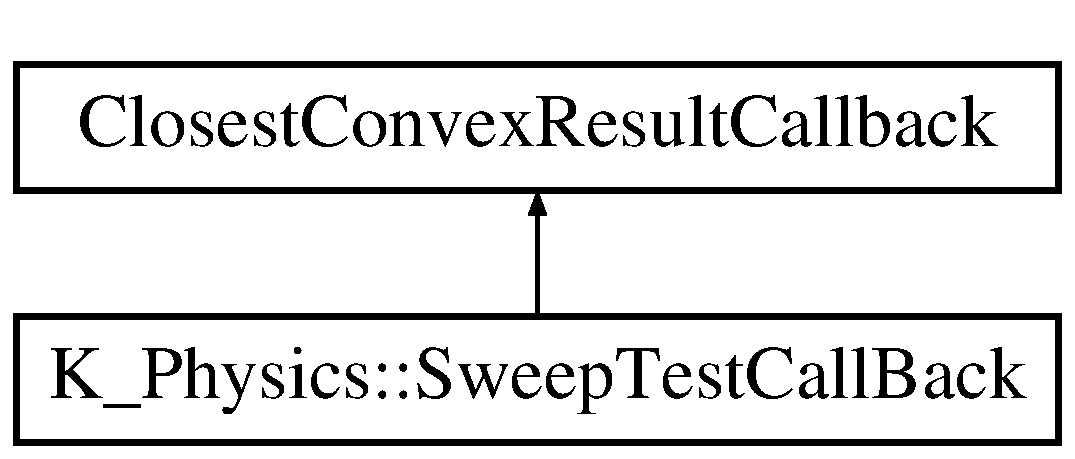
\includegraphics[height=2.000000cm]{struct_k___physics_1_1_sweep_test_call_back}
\end{center}
\end{figure}
\subsection*{公開メンバ関数}
\begin{DoxyCompactItemize}
\item 
\mbox{\hyperlink{struct_k___physics_1_1_sweep_test_call_back_ae8598d49a8cfdd4d2a9ed29c70db6f49}{Sweep\+Test\+Call\+Back}} (bt\+Collision\+Object $\ast$\mbox{\hyperlink{struct_k___physics_1_1_sweep_test_call_back_a54d36f38158c77a8aeca7aa015d255b5}{myself}})
\item 
virtual bt\+Scalar \mbox{\hyperlink{struct_k___physics_1_1_sweep_test_call_back_a1832e2d592d2161787bfc22377069446}{add\+Single\+Result}} (bt\+Collision\+World\+::\+Local\+Convex\+Result \&convex\+Result, bool normal\+In\+World\+Space)
\end{DoxyCompactItemize}
\subsection*{公開変数類}
\begin{DoxyCompactItemize}
\item 
bt\+Collision\+Object $\ast$ \mbox{\hyperlink{struct_k___physics_1_1_sweep_test_call_back_a54d36f38158c77a8aeca7aa015d255b5}{myself}}
\end{DoxyCompactItemize}


\subsection{構築子と解体子}
\mbox{\Hypertarget{struct_k___physics_1_1_sweep_test_call_back_ae8598d49a8cfdd4d2a9ed29c70db6f49}\label{struct_k___physics_1_1_sweep_test_call_back_ae8598d49a8cfdd4d2a9ed29c70db6f49}} 
\index{K\+\_\+\+Physics\+::\+Sweep\+Test\+Call\+Back@{K\+\_\+\+Physics\+::\+Sweep\+Test\+Call\+Back}!Sweep\+Test\+Call\+Back@{Sweep\+Test\+Call\+Back}}
\index{Sweep\+Test\+Call\+Back@{Sweep\+Test\+Call\+Back}!K\+\_\+\+Physics\+::\+Sweep\+Test\+Call\+Back@{K\+\_\+\+Physics\+::\+Sweep\+Test\+Call\+Back}}
\subsubsection{\texorpdfstring{Sweep\+Test\+Call\+Back()}{SweepTestCallBack()}}
{\footnotesize\ttfamily K\+\_\+\+Physics\+::\+Sweep\+Test\+Call\+Back\+::\+Sweep\+Test\+Call\+Back (\begin{DoxyParamCaption}\item[{bt\+Collision\+Object $\ast$}]{myself }\end{DoxyParamCaption})}



\subsection{関数詳解}
\mbox{\Hypertarget{struct_k___physics_1_1_sweep_test_call_back_a1832e2d592d2161787bfc22377069446}\label{struct_k___physics_1_1_sweep_test_call_back_a1832e2d592d2161787bfc22377069446}} 
\index{K\+\_\+\+Physics\+::\+Sweep\+Test\+Call\+Back@{K\+\_\+\+Physics\+::\+Sweep\+Test\+Call\+Back}!add\+Single\+Result@{add\+Single\+Result}}
\index{add\+Single\+Result@{add\+Single\+Result}!K\+\_\+\+Physics\+::\+Sweep\+Test\+Call\+Back@{K\+\_\+\+Physics\+::\+Sweep\+Test\+Call\+Back}}
\subsubsection{\texorpdfstring{add\+Single\+Result()}{addSingleResult()}}
{\footnotesize\ttfamily bt\+Scalar K\+\_\+\+Physics\+::\+Sweep\+Test\+Call\+Back\+::add\+Single\+Result (\begin{DoxyParamCaption}\item[{bt\+Collision\+World\+::\+Local\+Convex\+Result \&}]{convex\+Result,  }\item[{bool}]{normal\+In\+World\+Space }\end{DoxyParamCaption})\hspace{0.3cm}{\ttfamily [virtual]}}



\subsection{メンバ詳解}
\mbox{\Hypertarget{struct_k___physics_1_1_sweep_test_call_back_a54d36f38158c77a8aeca7aa015d255b5}\label{struct_k___physics_1_1_sweep_test_call_back_a54d36f38158c77a8aeca7aa015d255b5}} 
\index{K\+\_\+\+Physics\+::\+Sweep\+Test\+Call\+Back@{K\+\_\+\+Physics\+::\+Sweep\+Test\+Call\+Back}!myself@{myself}}
\index{myself@{myself}!K\+\_\+\+Physics\+::\+Sweep\+Test\+Call\+Back@{K\+\_\+\+Physics\+::\+Sweep\+Test\+Call\+Back}}
\subsubsection{\texorpdfstring{myself}{myself}}
{\footnotesize\ttfamily bt\+Collision\+Object$\ast$ K\+\_\+\+Physics\+::\+Sweep\+Test\+Call\+Back\+::myself}


\hypertarget{class_k___system_1_1_system_class}{}\section{K\+\_\+\+System\+:\+:System\+Class クラス}
\label{class_k___system_1_1_system_class}\index{K\+\_\+\+System\+::\+System\+Class@{K\+\_\+\+System\+::\+System\+Class}}


{\ttfamily \#include $<$System\+Class.\+h$>$}

\subsection*{公開メンバ関数}
\begin{DoxyCompactItemize}
\item 
\mbox{\hyperlink{class_k___system_1_1_system_class_a0202cc960e52ef4b51f0decb3c3fb35d}{System\+Class}} (int window\+Width, int window\+Height, bool is\+Full\+Screen)
\begin{DoxyCompactList}\small\item\em \mbox{\hyperlink{class_k___system_1_1_system_class_a2db013b3b45f150df5355fd5265c8705}{Initialize()}}を呼ぶ \end{DoxyCompactList}\item 
\mbox{\hyperlink{class_k___system_1_1_system_class_a5bdd9b6b328727510a660dc7ab9ea8ac}{$\sim$\+System\+Class}} ()
\begin{DoxyCompactList}\small\item\em \mbox{\hyperlink{class_k___system_1_1_system_class_a93d05d4f421da35f53c4969e53ca7d49}{Finalize()}}を呼ぶ \end{DoxyCompactList}\item 
bool \mbox{\hyperlink{class_k___system_1_1_system_class_a2db013b3b45f150df5355fd5265c8705}{Initialize}} (int window\+Width, int window\+Height, bool is\+Full\+Screen)
\begin{DoxyCompactList}\small\item\em 描画周りの初期化 \end{DoxyCompactList}\item 
void \mbox{\hyperlink{class_k___system_1_1_system_class_a93d05d4f421da35f53c4969e53ca7d49}{Finalize}} ()
\begin{DoxyCompactList}\small\item\em 終了処理、\+Initialize()の初めにも呼ばれている \end{DoxyCompactList}\item 
void \mbox{\hyperlink{class_k___system_1_1_system_class_a242be8d90313c17762b0013c30cafa47}{Process\+System}} ()
\begin{DoxyCompactList}\small\item\em ウィンドウイベントと入力の更新処理を行う \end{DoxyCompactList}\item 
void \mbox{\hyperlink{class_k___system_1_1_system_class_afe66afc17d7cad5199f4e8a1dd62b472}{Swap\+Buffer}} ()
\begin{DoxyCompactList}\small\item\em 描画を反映、これを呼ぶとフレームレートが60\+F\+P\+Sになる \end{DoxyCompactList}\item 
bool \mbox{\hyperlink{class_k___system_1_1_system_class_ab36bf9672ef9967b829b95da744c5394}{Window\+Forcus}} ()
\begin{DoxyCompactList}\small\item\em ウィンドウがフォーカスされているか \end{DoxyCompactList}\item 
bool \mbox{\hyperlink{class_k___system_1_1_system_class_a5c776515e01bcba724c6fa64db4897c0}{Is\+System\+End}} ()
\begin{DoxyCompactList}\small\item\em アプリの終了通知 \end{DoxyCompactList}\item 
int \mbox{\hyperlink{class_k___system_1_1_system_class_a8b1226fbf696428544adfa890430cac1}{Get\+Window\+Width}} ()
\begin{DoxyCompactList}\small\item\em アクセサー \end{DoxyCompactList}\item 
int \mbox{\hyperlink{class_k___system_1_1_system_class_a77b2bd403ce58a63f48151054ee2402e}{Get\+Window\+Height}} ()
\begin{DoxyCompactList}\small\item\em アクセサー \end{DoxyCompactList}\item 
\mbox{\hyperlink{class_k___input_1_1_input_g_l_f_w}{K\+\_\+\+Input\+::\+Input\+G\+L\+FW}} $\ast$ \mbox{\hyperlink{class_k___system_1_1_system_class_ac4f7977cb0325fe9ac581ed1942404a0}{Get\+Input}} ()
\begin{DoxyCompactList}\small\item\em アクセサー \end{DoxyCompactList}\end{DoxyCompactItemize}


\subsection{詳解}
アプリケーションの動作を管理

一番初めに初期化し、\+Is\+System\+End()がtrueになるまでの間アプリケーションを動かす~\newline
なお、「キー入力・ゲームパッド入力」の情報はこのクラスにある 

\subsection{構築子と解体子}
\mbox{\Hypertarget{class_k___system_1_1_system_class_a0202cc960e52ef4b51f0decb3c3fb35d}\label{class_k___system_1_1_system_class_a0202cc960e52ef4b51f0decb3c3fb35d}} 
\index{K\+\_\+\+System\+::\+System\+Class@{K\+\_\+\+System\+::\+System\+Class}!System\+Class@{System\+Class}}
\index{System\+Class@{System\+Class}!K\+\_\+\+System\+::\+System\+Class@{K\+\_\+\+System\+::\+System\+Class}}
\subsubsection{\texorpdfstring{System\+Class()}{SystemClass()}}
{\footnotesize\ttfamily K\+\_\+\+System\+::\+System\+Class\+::\+System\+Class (\begin{DoxyParamCaption}\item[{int}]{window\+Width,  }\item[{int}]{window\+Height,  }\item[{bool}]{is\+Full\+Screen }\end{DoxyParamCaption})}



\mbox{\hyperlink{class_k___system_1_1_system_class_a2db013b3b45f150df5355fd5265c8705}{Initialize()}}を呼ぶ 

\mbox{\Hypertarget{class_k___system_1_1_system_class_a5bdd9b6b328727510a660dc7ab9ea8ac}\label{class_k___system_1_1_system_class_a5bdd9b6b328727510a660dc7ab9ea8ac}} 
\index{K\+\_\+\+System\+::\+System\+Class@{K\+\_\+\+System\+::\+System\+Class}!````~System\+Class@{$\sim$\+System\+Class}}
\index{````~System\+Class@{$\sim$\+System\+Class}!K\+\_\+\+System\+::\+System\+Class@{K\+\_\+\+System\+::\+System\+Class}}
\subsubsection{\texorpdfstring{$\sim$\+System\+Class()}{~SystemClass()}}
{\footnotesize\ttfamily K\+\_\+\+System\+::\+System\+Class\+::$\sim$\+System\+Class (\begin{DoxyParamCaption}{ }\end{DoxyParamCaption})}



\mbox{\hyperlink{class_k___system_1_1_system_class_a93d05d4f421da35f53c4969e53ca7d49}{Finalize()}}を呼ぶ 



\subsection{関数詳解}
\mbox{\Hypertarget{class_k___system_1_1_system_class_a93d05d4f421da35f53c4969e53ca7d49}\label{class_k___system_1_1_system_class_a93d05d4f421da35f53c4969e53ca7d49}} 
\index{K\+\_\+\+System\+::\+System\+Class@{K\+\_\+\+System\+::\+System\+Class}!Finalize@{Finalize}}
\index{Finalize@{Finalize}!K\+\_\+\+System\+::\+System\+Class@{K\+\_\+\+System\+::\+System\+Class}}
\subsubsection{\texorpdfstring{Finalize()}{Finalize()}}
{\footnotesize\ttfamily void K\+\_\+\+System\+::\+System\+Class\+::\+Finalize (\begin{DoxyParamCaption}{ }\end{DoxyParamCaption})}



終了処理、\+Initialize()の初めにも呼ばれている 

\mbox{\Hypertarget{class_k___system_1_1_system_class_ac4f7977cb0325fe9ac581ed1942404a0}\label{class_k___system_1_1_system_class_ac4f7977cb0325fe9ac581ed1942404a0}} 
\index{K\+\_\+\+System\+::\+System\+Class@{K\+\_\+\+System\+::\+System\+Class}!Get\+Input@{Get\+Input}}
\index{Get\+Input@{Get\+Input}!K\+\_\+\+System\+::\+System\+Class@{K\+\_\+\+System\+::\+System\+Class}}
\subsubsection{\texorpdfstring{Get\+Input()}{GetInput()}}
{\footnotesize\ttfamily \mbox{\hyperlink{class_k___input_1_1_input_g_l_f_w}{K\+\_\+\+Input\+::\+Input\+G\+L\+FW}} $\ast$ K\+\_\+\+System\+::\+System\+Class\+::\+Get\+Input (\begin{DoxyParamCaption}{ }\end{DoxyParamCaption})}



アクセサー 

\begin{DoxyReturn}{戻り値}
入力クラスへのポインタ 
\end{DoxyReturn}
\mbox{\Hypertarget{class_k___system_1_1_system_class_a77b2bd403ce58a63f48151054ee2402e}\label{class_k___system_1_1_system_class_a77b2bd403ce58a63f48151054ee2402e}} 
\index{K\+\_\+\+System\+::\+System\+Class@{K\+\_\+\+System\+::\+System\+Class}!Get\+Window\+Height@{Get\+Window\+Height}}
\index{Get\+Window\+Height@{Get\+Window\+Height}!K\+\_\+\+System\+::\+System\+Class@{K\+\_\+\+System\+::\+System\+Class}}
\subsubsection{\texorpdfstring{Get\+Window\+Height()}{GetWindowHeight()}}
{\footnotesize\ttfamily int K\+\_\+\+System\+::\+System\+Class\+::\+Get\+Window\+Height (\begin{DoxyParamCaption}{ }\end{DoxyParamCaption})}



アクセサー 

\begin{DoxyReturn}{戻り値}
ウィンドウの高さ 
\end{DoxyReturn}
\mbox{\Hypertarget{class_k___system_1_1_system_class_a8b1226fbf696428544adfa890430cac1}\label{class_k___system_1_1_system_class_a8b1226fbf696428544adfa890430cac1}} 
\index{K\+\_\+\+System\+::\+System\+Class@{K\+\_\+\+System\+::\+System\+Class}!Get\+Window\+Width@{Get\+Window\+Width}}
\index{Get\+Window\+Width@{Get\+Window\+Width}!K\+\_\+\+System\+::\+System\+Class@{K\+\_\+\+System\+::\+System\+Class}}
\subsubsection{\texorpdfstring{Get\+Window\+Width()}{GetWindowWidth()}}
{\footnotesize\ttfamily int K\+\_\+\+System\+::\+System\+Class\+::\+Get\+Window\+Width (\begin{DoxyParamCaption}{ }\end{DoxyParamCaption})}



アクセサー 

\begin{DoxyReturn}{戻り値}
ウィンドウの幅 
\end{DoxyReturn}
\mbox{\Hypertarget{class_k___system_1_1_system_class_a2db013b3b45f150df5355fd5265c8705}\label{class_k___system_1_1_system_class_a2db013b3b45f150df5355fd5265c8705}} 
\index{K\+\_\+\+System\+::\+System\+Class@{K\+\_\+\+System\+::\+System\+Class}!Initialize@{Initialize}}
\index{Initialize@{Initialize}!K\+\_\+\+System\+::\+System\+Class@{K\+\_\+\+System\+::\+System\+Class}}
\subsubsection{\texorpdfstring{Initialize()}{Initialize()}}
{\footnotesize\ttfamily bool K\+\_\+\+System\+::\+System\+Class\+::\+Initialize (\begin{DoxyParamCaption}\item[{int}]{window\+Width,  }\item[{int}]{window\+Height,  }\item[{bool}]{is\+Full\+Screen }\end{DoxyParamCaption})}



描画周りの初期化 


\begin{DoxyParams}[1]{引数}
\mbox{\tt in}  & {\em window\+Width} & 作成するウィンドウの幅 \\
\hline
\mbox{\tt in}  & {\em window\+Height} & 作成するウィンドウの高さ \\
\hline
\mbox{\tt in}  & {\em is\+Full\+Screen} & フルスクリーンにするか(ウィンドウのサイズが解像度になります) \\
\hline
\end{DoxyParams}
\begin{DoxyReturn}{戻り値}
初期化に成功するとtrue 
\end{DoxyReturn}
\mbox{\Hypertarget{class_k___system_1_1_system_class_a5c776515e01bcba724c6fa64db4897c0}\label{class_k___system_1_1_system_class_a5c776515e01bcba724c6fa64db4897c0}} 
\index{K\+\_\+\+System\+::\+System\+Class@{K\+\_\+\+System\+::\+System\+Class}!Is\+System\+End@{Is\+System\+End}}
\index{Is\+System\+End@{Is\+System\+End}!K\+\_\+\+System\+::\+System\+Class@{K\+\_\+\+System\+::\+System\+Class}}
\subsubsection{\texorpdfstring{Is\+System\+End()}{IsSystemEnd()}}
{\footnotesize\ttfamily bool K\+\_\+\+System\+::\+System\+Class\+::\+Is\+System\+End (\begin{DoxyParamCaption}{ }\end{DoxyParamCaption})}



アプリの終了通知 

\begin{DoxyReturn}{戻り値}
ウィンドウが閉じられたり、\+Escキーが押下されたときにtrue 
\end{DoxyReturn}
\mbox{\Hypertarget{class_k___system_1_1_system_class_a242be8d90313c17762b0013c30cafa47}\label{class_k___system_1_1_system_class_a242be8d90313c17762b0013c30cafa47}} 
\index{K\+\_\+\+System\+::\+System\+Class@{K\+\_\+\+System\+::\+System\+Class}!Process\+System@{Process\+System}}
\index{Process\+System@{Process\+System}!K\+\_\+\+System\+::\+System\+Class@{K\+\_\+\+System\+::\+System\+Class}}
\subsubsection{\texorpdfstring{Process\+System()}{ProcessSystem()}}
{\footnotesize\ttfamily void K\+\_\+\+System\+::\+System\+Class\+::\+Process\+System (\begin{DoxyParamCaption}{ }\end{DoxyParamCaption})}



ウィンドウイベントと入力の更新処理を行う 

\mbox{\Hypertarget{class_k___system_1_1_system_class_afe66afc17d7cad5199f4e8a1dd62b472}\label{class_k___system_1_1_system_class_afe66afc17d7cad5199f4e8a1dd62b472}} 
\index{K\+\_\+\+System\+::\+System\+Class@{K\+\_\+\+System\+::\+System\+Class}!Swap\+Buffer@{Swap\+Buffer}}
\index{Swap\+Buffer@{Swap\+Buffer}!K\+\_\+\+System\+::\+System\+Class@{K\+\_\+\+System\+::\+System\+Class}}
\subsubsection{\texorpdfstring{Swap\+Buffer()}{SwapBuffer()}}
{\footnotesize\ttfamily void K\+\_\+\+System\+::\+System\+Class\+::\+Swap\+Buffer (\begin{DoxyParamCaption}{ }\end{DoxyParamCaption})}



描画を反映、これを呼ぶとフレームレートが60\+F\+P\+Sになる 

\mbox{\Hypertarget{class_k___system_1_1_system_class_ab36bf9672ef9967b829b95da744c5394}\label{class_k___system_1_1_system_class_ab36bf9672ef9967b829b95da744c5394}} 
\index{K\+\_\+\+System\+::\+System\+Class@{K\+\_\+\+System\+::\+System\+Class}!Window\+Forcus@{Window\+Forcus}}
\index{Window\+Forcus@{Window\+Forcus}!K\+\_\+\+System\+::\+System\+Class@{K\+\_\+\+System\+::\+System\+Class}}
\subsubsection{\texorpdfstring{Window\+Forcus()}{WindowForcus()}}
{\footnotesize\ttfamily bool K\+\_\+\+System\+::\+System\+Class\+::\+Window\+Forcus (\begin{DoxyParamCaption}{ }\end{DoxyParamCaption})}



ウィンドウがフォーカスされているか 

\begin{DoxyReturn}{戻り値}
ウィンドウがフォーカスされているときtrue 
\end{DoxyReturn}

\hypertarget{class_k___graphics_1_1_texture}{}\section{K\+\_\+\+Graphics\+:\+:Texture クラス}
\label{class_k___graphics_1_1_texture}\index{K\+\_\+\+Graphics\+::\+Texture@{K\+\_\+\+Graphics\+::\+Texture}}


外部から読み込まれた、あるいは作られたテクスチャを保持する~\newline
このクラスは、保持しているテクスチャの解放責任を持つ  




{\ttfamily \#include $<$Texture.\+h$>$}

\subsection*{公開メンバ関数}
\begin{DoxyCompactItemize}
\item 
\mbox{\hyperlink{class_k___graphics_1_1_texture_a3d4fc11068626d4d981b37d1d5aead47}{Texture}} ()
\begin{DoxyCompactList}\small\item\em \mbox{\hyperlink{class_k___graphics_1_1_texture_a569217a622e060f157842e5d492b8b34}{Initialize()}}を呼ぶ \end{DoxyCompactList}\item 
\mbox{\hyperlink{class_k___graphics_1_1_texture_aacbb913221bc16ca6b1b2d8f8a62fc60}{$\sim$\+Texture}} ()
\begin{DoxyCompactList}\small\item\em テクスチャを開放する \end{DoxyCompactList}\item 
bool \mbox{\hyperlink{class_k___graphics_1_1_texture_a569217a622e060f157842e5d492b8b34}{Initialize}} ()
\begin{DoxyCompactList}\small\item\em 空のデータでテクスチャを初期化 \end{DoxyCompactList}\item 
bool \mbox{\hyperlink{class_k___graphics_1_1_texture_a3f4839ab22e8a2e9aeb58ae49509f73d}{Load\+Image}} (const std\+::string \&file\+Name)
\begin{DoxyCompactList}\small\item\em 画像を読み込んでテクスチャに渡す \end{DoxyCompactList}\item 
void \mbox{\hyperlink{class_k___graphics_1_1_texture_a07e94ca2f5d93698ad168ac15e3cc2dd}{Set\+Image\+Data}} (void $\ast$data, int width, int height, \mbox{\hyperlink{namespace_k___graphics_a218722f1def83362c6b74680b8c1c529}{Texture\+Type}} b\+Type, \mbox{\hyperlink{namespace_k___graphics_a9654dafb2cd6eaed24a292a6f8373955}{Texture\+Color\+Type}} texture\+Color, \mbox{\hyperlink{namespace_k___graphics_a9654dafb2cd6eaed24a292a6f8373955}{Texture\+Color\+Type}} data\+Color)
\begin{DoxyCompactList}\small\item\em 配列データを画像として渡す \end{DoxyCompactList}\item 
void \mbox{\hyperlink{class_k___graphics_1_1_texture_ada11b0ac5f51e73ca07dc2a69fb32e3c}{Set\+Filter}} (bool is\+Filtering)
\begin{DoxyCompactList}\small\item\em 画像の拡縮時にフィルターをかけるか設定 \end{DoxyCompactList}\item 
G\+Luint \mbox{\hyperlink{class_k___graphics_1_1_texture_ab37df6d52bfb67f14065f1d8f26c3472}{Get\+Texture\+ID}} ()
\item 
unsigned int \mbox{\hyperlink{class_k___graphics_1_1_texture_ad5085a98a35f04eaf532e2a2acdf672d}{Get\+Width}} ()
\item 
unsigned int \mbox{\hyperlink{class_k___graphics_1_1_texture_a6e7ba63d4782a62b055474945578fae9}{Get\+Height}} ()
\end{DoxyCompactItemize}


\subsection{詳解}
外部から読み込まれた、あるいは作られたテクスチャを保持する~\newline
このクラスは、保持しているテクスチャの解放責任を持つ 

\subsection{構築子と解体子}
\mbox{\Hypertarget{class_k___graphics_1_1_texture_a3d4fc11068626d4d981b37d1d5aead47}\label{class_k___graphics_1_1_texture_a3d4fc11068626d4d981b37d1d5aead47}} 
\index{K\+\_\+\+Graphics\+::\+Texture@{K\+\_\+\+Graphics\+::\+Texture}!Texture@{Texture}}
\index{Texture@{Texture}!K\+\_\+\+Graphics\+::\+Texture@{K\+\_\+\+Graphics\+::\+Texture}}
\subsubsection{\texorpdfstring{Texture()}{Texture()}}
{\footnotesize\ttfamily K\+\_\+\+Graphics\+::\+Texture\+::\+Texture (\begin{DoxyParamCaption}{ }\end{DoxyParamCaption})}



\mbox{\hyperlink{class_k___graphics_1_1_texture_a569217a622e060f157842e5d492b8b34}{Initialize()}}を呼ぶ 

\mbox{\Hypertarget{class_k___graphics_1_1_texture_aacbb913221bc16ca6b1b2d8f8a62fc60}\label{class_k___graphics_1_1_texture_aacbb913221bc16ca6b1b2d8f8a62fc60}} 
\index{K\+\_\+\+Graphics\+::\+Texture@{K\+\_\+\+Graphics\+::\+Texture}!````~Texture@{$\sim$\+Texture}}
\index{````~Texture@{$\sim$\+Texture}!K\+\_\+\+Graphics\+::\+Texture@{K\+\_\+\+Graphics\+::\+Texture}}
\subsubsection{\texorpdfstring{$\sim$\+Texture()}{~Texture()}}
{\footnotesize\ttfamily K\+\_\+\+Graphics\+::\+Texture\+::$\sim$\+Texture (\begin{DoxyParamCaption}{ }\end{DoxyParamCaption})}



テクスチャを開放する 



\subsection{関数詳解}
\mbox{\Hypertarget{class_k___graphics_1_1_texture_a6e7ba63d4782a62b055474945578fae9}\label{class_k___graphics_1_1_texture_a6e7ba63d4782a62b055474945578fae9}} 
\index{K\+\_\+\+Graphics\+::\+Texture@{K\+\_\+\+Graphics\+::\+Texture}!Get\+Height@{Get\+Height}}
\index{Get\+Height@{Get\+Height}!K\+\_\+\+Graphics\+::\+Texture@{K\+\_\+\+Graphics\+::\+Texture}}
\subsubsection{\texorpdfstring{Get\+Height()}{GetHeight()}}
{\footnotesize\ttfamily unsigned int K\+\_\+\+Graphics\+::\+Texture\+::\+Get\+Height (\begin{DoxyParamCaption}{ }\end{DoxyParamCaption})}

\begin{DoxyReturn}{戻り値}
テクスチャ画像高さ 
\end{DoxyReturn}
\mbox{\Hypertarget{class_k___graphics_1_1_texture_ab37df6d52bfb67f14065f1d8f26c3472}\label{class_k___graphics_1_1_texture_ab37df6d52bfb67f14065f1d8f26c3472}} 
\index{K\+\_\+\+Graphics\+::\+Texture@{K\+\_\+\+Graphics\+::\+Texture}!Get\+Texture\+ID@{Get\+Texture\+ID}}
\index{Get\+Texture\+ID@{Get\+Texture\+ID}!K\+\_\+\+Graphics\+::\+Texture@{K\+\_\+\+Graphics\+::\+Texture}}
\subsubsection{\texorpdfstring{Get\+Texture\+I\+D()}{GetTextureID()}}
{\footnotesize\ttfamily G\+Luint K\+\_\+\+Graphics\+::\+Texture\+::\+Get\+Texture\+ID (\begin{DoxyParamCaption}{ }\end{DoxyParamCaption})}

\begin{DoxyReturn}{戻り値}
シェーダーに渡す際のテクスチャインデックス 
\end{DoxyReturn}
\mbox{\Hypertarget{class_k___graphics_1_1_texture_ad5085a98a35f04eaf532e2a2acdf672d}\label{class_k___graphics_1_1_texture_ad5085a98a35f04eaf532e2a2acdf672d}} 
\index{K\+\_\+\+Graphics\+::\+Texture@{K\+\_\+\+Graphics\+::\+Texture}!Get\+Width@{Get\+Width}}
\index{Get\+Width@{Get\+Width}!K\+\_\+\+Graphics\+::\+Texture@{K\+\_\+\+Graphics\+::\+Texture}}
\subsubsection{\texorpdfstring{Get\+Width()}{GetWidth()}}
{\footnotesize\ttfamily unsigned int K\+\_\+\+Graphics\+::\+Texture\+::\+Get\+Width (\begin{DoxyParamCaption}{ }\end{DoxyParamCaption})}

\begin{DoxyReturn}{戻り値}
テクスチャ画像幅 
\end{DoxyReturn}
\mbox{\Hypertarget{class_k___graphics_1_1_texture_a569217a622e060f157842e5d492b8b34}\label{class_k___graphics_1_1_texture_a569217a622e060f157842e5d492b8b34}} 
\index{K\+\_\+\+Graphics\+::\+Texture@{K\+\_\+\+Graphics\+::\+Texture}!Initialize@{Initialize}}
\index{Initialize@{Initialize}!K\+\_\+\+Graphics\+::\+Texture@{K\+\_\+\+Graphics\+::\+Texture}}
\subsubsection{\texorpdfstring{Initialize()}{Initialize()}}
{\footnotesize\ttfamily bool K\+\_\+\+Graphics\+::\+Texture\+::\+Initialize (\begin{DoxyParamCaption}{ }\end{DoxyParamCaption})}



空のデータでテクスチャを初期化 

\mbox{\Hypertarget{class_k___graphics_1_1_texture_a3f4839ab22e8a2e9aeb58ae49509f73d}\label{class_k___graphics_1_1_texture_a3f4839ab22e8a2e9aeb58ae49509f73d}} 
\index{K\+\_\+\+Graphics\+::\+Texture@{K\+\_\+\+Graphics\+::\+Texture}!Load\+Image@{Load\+Image}}
\index{Load\+Image@{Load\+Image}!K\+\_\+\+Graphics\+::\+Texture@{K\+\_\+\+Graphics\+::\+Texture}}
\subsubsection{\texorpdfstring{Load\+Image()}{LoadImage()}}
{\footnotesize\ttfamily bool K\+\_\+\+Graphics\+::\+Texture\+::\+Load\+Image (\begin{DoxyParamCaption}\item[{const std\+::string \&}]{file\+Name }\end{DoxyParamCaption})}



画像を読み込んでテクスチャに渡す 


\begin{DoxyParams}{引数}
{\em file\+Name} & 画像のファイルパス \\
\hline
\end{DoxyParams}
\begin{DoxyReturn}{戻り値}
成功するとtrue 
\end{DoxyReturn}
\mbox{\Hypertarget{class_k___graphics_1_1_texture_ada11b0ac5f51e73ca07dc2a69fb32e3c}\label{class_k___graphics_1_1_texture_ada11b0ac5f51e73ca07dc2a69fb32e3c}} 
\index{K\+\_\+\+Graphics\+::\+Texture@{K\+\_\+\+Graphics\+::\+Texture}!Set\+Filter@{Set\+Filter}}
\index{Set\+Filter@{Set\+Filter}!K\+\_\+\+Graphics\+::\+Texture@{K\+\_\+\+Graphics\+::\+Texture}}
\subsubsection{\texorpdfstring{Set\+Filter()}{SetFilter()}}
{\footnotesize\ttfamily void K\+\_\+\+Graphics\+::\+Texture\+::\+Set\+Filter (\begin{DoxyParamCaption}\item[{bool}]{is\+Filtering }\end{DoxyParamCaption})}



画像の拡縮時にフィルターをかけるか設定 


\begin{DoxyParams}[1]{引数}
\mbox{\tt in}  & {\em is\+Filtering} & フィルタリングをするかのフラグ \\
\hline
\end{DoxyParams}
\mbox{\Hypertarget{class_k___graphics_1_1_texture_a07e94ca2f5d93698ad168ac15e3cc2dd}\label{class_k___graphics_1_1_texture_a07e94ca2f5d93698ad168ac15e3cc2dd}} 
\index{K\+\_\+\+Graphics\+::\+Texture@{K\+\_\+\+Graphics\+::\+Texture}!Set\+Image\+Data@{Set\+Image\+Data}}
\index{Set\+Image\+Data@{Set\+Image\+Data}!K\+\_\+\+Graphics\+::\+Texture@{K\+\_\+\+Graphics\+::\+Texture}}
\subsubsection{\texorpdfstring{Set\+Image\+Data()}{SetImageData()}}
{\footnotesize\ttfamily void K\+\_\+\+Graphics\+::\+Texture\+::\+Set\+Image\+Data (\begin{DoxyParamCaption}\item[{void $\ast$}]{data,  }\item[{int}]{width,  }\item[{int}]{height,  }\item[{\mbox{\hyperlink{namespace_k___graphics_a218722f1def83362c6b74680b8c1c529}{Texture\+Type}}}]{b\+Type,  }\item[{\mbox{\hyperlink{namespace_k___graphics_a9654dafb2cd6eaed24a292a6f8373955}{Texture\+Color\+Type}}}]{texture\+Color,  }\item[{\mbox{\hyperlink{namespace_k___graphics_a9654dafb2cd6eaed24a292a6f8373955}{Texture\+Color\+Type}}}]{data\+Color }\end{DoxyParamCaption})}



配列データを画像として渡す 


\begin{DoxyParams}[1]{引数}
\mbox{\tt in}  & {\em data} & データの入った配列 \\
\hline
\mbox{\tt in}  & {\em width} & 画像幅 \\
\hline
\mbox{\tt in}  & {\em height} & 画像高さ \\
\hline
\mbox{\tt in}  & {\em b\+Type} & テクスチャの数値型の設定 \\
\hline
\mbox{\tt in}  & {\em texture\+Color} & テクスチャの色の形式 \\
\hline
\mbox{\tt in}  & {\em data\+Color} & テクスチャが利用する画像の色の形式 \\
\hline
\end{DoxyParams}

\hypertarget{class_k___graphics_1_1_texture_list}{}\section{K\+\_\+\+Graphics\+:\+:Texture\+List クラス}
\label{class_k___graphics_1_1_texture_list}\index{K\+\_\+\+Graphics\+::\+Texture\+List@{K\+\_\+\+Graphics\+::\+Texture\+List}}


テクスチャクラスをリストとして持ち、解放責任をもつクラス  




{\ttfamily \#include $<$Texture\+List.\+h$>$}

\subsection*{公開メンバ関数}
\begin{DoxyCompactItemize}
\item 
\mbox{\hyperlink{class_k___graphics_1_1_texture_list_a32733fdf9b63714a2730fccfe6d4d39b}{Texture\+List}} ()
\begin{DoxyCompactList}\small\item\em \mbox{\hyperlink{class_k___graphics_1_1_texture_list_a82c3a0615564dc2f016132b001093014}{Initialize()}}を呼ぶ \end{DoxyCompactList}\item 
\mbox{\hyperlink{class_k___graphics_1_1_texture_list_ad96337c9c60f13d1f6f9e088cab90ffc}{$\sim$\+Texture\+List}} ()
\begin{DoxyCompactList}\small\item\em \mbox{\hyperlink{class_k___graphics_1_1_texture_list_a82c3a0615564dc2f016132b001093014}{Initialize()}}を呼ぶ \end{DoxyCompactList}\item 
void \mbox{\hyperlink{class_k___graphics_1_1_texture_list_a82c3a0615564dc2f016132b001093014}{Initialize}} ()
\begin{DoxyCompactList}\small\item\em リストのテクスチャを全て開放する \end{DoxyCompactList}\item 
\mbox{\hyperlink{class_k___graphics_1_1_texture}{Texture}} $\ast$ \mbox{\hyperlink{class_k___graphics_1_1_texture_list_a71d4ef3f54b37dbc4b0c65e7b981678a}{Get\+Texture}} (const std\+::string \&texture\+Name)
\begin{DoxyCompactList}\small\item\em テクスチャを取得 \end{DoxyCompactList}\item 
bool \mbox{\hyperlink{class_k___graphics_1_1_texture_list_ab743facbd1bda2b2bc665171bdb34b48}{Load\+Texture}} (const std\+::string \&texture\+Name, const std\+::string \&file\+Pass)
\begin{DoxyCompactList}\small\item\em テクスチャ読み込み \end{DoxyCompactList}\item 
bool \mbox{\hyperlink{class_k___graphics_1_1_texture_list_afab7447d6ed329a257436a20aad2cae3}{Add\+Empty\+Texture}} (const std\+::string \&texture\+Name, int texture\+Width, int texture\+Height)
\begin{DoxyCompactList}\small\item\em 空のテクスチャを作成 \end{DoxyCompactList}\item 
void \mbox{\hyperlink{class_k___graphics_1_1_texture_list_af5823a146cd8494b261ddcdf0d515859}{Delete\+Texture}} (const std\+::string \&texture\+Name)
\begin{DoxyCompactList}\small\item\em テクスチャを削除 \end{DoxyCompactList}\end{DoxyCompactItemize}


\subsection{詳解}
テクスチャクラスをリストとして持ち、解放責任をもつクラス 

\subsection{構築子と解体子}
\mbox{\Hypertarget{class_k___graphics_1_1_texture_list_a32733fdf9b63714a2730fccfe6d4d39b}\label{class_k___graphics_1_1_texture_list_a32733fdf9b63714a2730fccfe6d4d39b}} 
\index{K\+\_\+\+Graphics\+::\+Texture\+List@{K\+\_\+\+Graphics\+::\+Texture\+List}!Texture\+List@{Texture\+List}}
\index{Texture\+List@{Texture\+List}!K\+\_\+\+Graphics\+::\+Texture\+List@{K\+\_\+\+Graphics\+::\+Texture\+List}}
\subsubsection{\texorpdfstring{Texture\+List()}{TextureList()}}
{\footnotesize\ttfamily K\+\_\+\+Graphics\+::\+Texture\+List\+::\+Texture\+List (\begin{DoxyParamCaption}{ }\end{DoxyParamCaption})}



\mbox{\hyperlink{class_k___graphics_1_1_texture_list_a82c3a0615564dc2f016132b001093014}{Initialize()}}を呼ぶ 

\mbox{\Hypertarget{class_k___graphics_1_1_texture_list_ad96337c9c60f13d1f6f9e088cab90ffc}\label{class_k___graphics_1_1_texture_list_ad96337c9c60f13d1f6f9e088cab90ffc}} 
\index{K\+\_\+\+Graphics\+::\+Texture\+List@{K\+\_\+\+Graphics\+::\+Texture\+List}!````~Texture\+List@{$\sim$\+Texture\+List}}
\index{````~Texture\+List@{$\sim$\+Texture\+List}!K\+\_\+\+Graphics\+::\+Texture\+List@{K\+\_\+\+Graphics\+::\+Texture\+List}}
\subsubsection{\texorpdfstring{$\sim$\+Texture\+List()}{~TextureList()}}
{\footnotesize\ttfamily K\+\_\+\+Graphics\+::\+Texture\+List\+::$\sim$\+Texture\+List (\begin{DoxyParamCaption}{ }\end{DoxyParamCaption})}



\mbox{\hyperlink{class_k___graphics_1_1_texture_list_a82c3a0615564dc2f016132b001093014}{Initialize()}}を呼ぶ 



\subsection{関数詳解}
\mbox{\Hypertarget{class_k___graphics_1_1_texture_list_afab7447d6ed329a257436a20aad2cae3}\label{class_k___graphics_1_1_texture_list_afab7447d6ed329a257436a20aad2cae3}} 
\index{K\+\_\+\+Graphics\+::\+Texture\+List@{K\+\_\+\+Graphics\+::\+Texture\+List}!Add\+Empty\+Texture@{Add\+Empty\+Texture}}
\index{Add\+Empty\+Texture@{Add\+Empty\+Texture}!K\+\_\+\+Graphics\+::\+Texture\+List@{K\+\_\+\+Graphics\+::\+Texture\+List}}
\subsubsection{\texorpdfstring{Add\+Empty\+Texture()}{AddEmptyTexture()}}
{\footnotesize\ttfamily bool K\+\_\+\+Graphics\+::\+Texture\+List\+::\+Add\+Empty\+Texture (\begin{DoxyParamCaption}\item[{const std\+::string \&}]{texture\+Name,  }\item[{int}]{texture\+Width,  }\item[{int}]{texture\+Height }\end{DoxyParamCaption})}



空のテクスチャを作成 


\begin{DoxyParams}[1]{引数}
\mbox{\tt in}  & {\em texture\+Name} & 作成するテクスチャのユーザー定義名 \\
\hline
\mbox{\tt in}  & {\em texture\+Width} & テクスチャの画像幅 \\
\hline
\mbox{\tt in}  & {\em texture\+Height} & テクスチャの画像高さ \\
\hline
\end{DoxyParams}
\begin{DoxyReturn}{戻り値}
成功するとtrue 
\end{DoxyReturn}
\mbox{\Hypertarget{class_k___graphics_1_1_texture_list_af5823a146cd8494b261ddcdf0d515859}\label{class_k___graphics_1_1_texture_list_af5823a146cd8494b261ddcdf0d515859}} 
\index{K\+\_\+\+Graphics\+::\+Texture\+List@{K\+\_\+\+Graphics\+::\+Texture\+List}!Delete\+Texture@{Delete\+Texture}}
\index{Delete\+Texture@{Delete\+Texture}!K\+\_\+\+Graphics\+::\+Texture\+List@{K\+\_\+\+Graphics\+::\+Texture\+List}}
\subsubsection{\texorpdfstring{Delete\+Texture()}{DeleteTexture()}}
{\footnotesize\ttfamily void K\+\_\+\+Graphics\+::\+Texture\+List\+::\+Delete\+Texture (\begin{DoxyParamCaption}\item[{const std\+::string \&}]{texture\+Name }\end{DoxyParamCaption})}



テクスチャを削除 


\begin{DoxyParams}[1]{引数}
\mbox{\tt in}  & {\em texture\+Name} & 削除するテクスチャの名前 \\
\hline
\end{DoxyParams}
\mbox{\Hypertarget{class_k___graphics_1_1_texture_list_a71d4ef3f54b37dbc4b0c65e7b981678a}\label{class_k___graphics_1_1_texture_list_a71d4ef3f54b37dbc4b0c65e7b981678a}} 
\index{K\+\_\+\+Graphics\+::\+Texture\+List@{K\+\_\+\+Graphics\+::\+Texture\+List}!Get\+Texture@{Get\+Texture}}
\index{Get\+Texture@{Get\+Texture}!K\+\_\+\+Graphics\+::\+Texture\+List@{K\+\_\+\+Graphics\+::\+Texture\+List}}
\subsubsection{\texorpdfstring{Get\+Texture()}{GetTexture()}}
{\footnotesize\ttfamily \mbox{\hyperlink{class_k___graphics_1_1_texture}{Texture}} $\ast$ K\+\_\+\+Graphics\+::\+Texture\+List\+::\+Get\+Texture (\begin{DoxyParamCaption}\item[{const std\+::string \&}]{texture\+Name }\end{DoxyParamCaption})}



テクスチャを取得 


\begin{DoxyParams}[1]{引数}
\mbox{\tt in}  & {\em texture\+Name} & テクスチャの名前 \\
\hline
\end{DoxyParams}
\begin{DoxyReturn}{戻り値}
その名前のテクスチャへのポインタ、無かったらnullptr 
\end{DoxyReturn}
\mbox{\Hypertarget{class_k___graphics_1_1_texture_list_a82c3a0615564dc2f016132b001093014}\label{class_k___graphics_1_1_texture_list_a82c3a0615564dc2f016132b001093014}} 
\index{K\+\_\+\+Graphics\+::\+Texture\+List@{K\+\_\+\+Graphics\+::\+Texture\+List}!Initialize@{Initialize}}
\index{Initialize@{Initialize}!K\+\_\+\+Graphics\+::\+Texture\+List@{K\+\_\+\+Graphics\+::\+Texture\+List}}
\subsubsection{\texorpdfstring{Initialize()}{Initialize()}}
{\footnotesize\ttfamily void K\+\_\+\+Graphics\+::\+Texture\+List\+::\+Initialize (\begin{DoxyParamCaption}{ }\end{DoxyParamCaption})}



リストのテクスチャを全て開放する 

\mbox{\Hypertarget{class_k___graphics_1_1_texture_list_ab743facbd1bda2b2bc665171bdb34b48}\label{class_k___graphics_1_1_texture_list_ab743facbd1bda2b2bc665171bdb34b48}} 
\index{K\+\_\+\+Graphics\+::\+Texture\+List@{K\+\_\+\+Graphics\+::\+Texture\+List}!Load\+Texture@{Load\+Texture}}
\index{Load\+Texture@{Load\+Texture}!K\+\_\+\+Graphics\+::\+Texture\+List@{K\+\_\+\+Graphics\+::\+Texture\+List}}
\subsubsection{\texorpdfstring{Load\+Texture()}{LoadTexture()}}
{\footnotesize\ttfamily bool K\+\_\+\+Graphics\+::\+Texture\+List\+::\+Load\+Texture (\begin{DoxyParamCaption}\item[{const std\+::string \&}]{texture\+Name,  }\item[{const std\+::string \&}]{file\+Pass }\end{DoxyParamCaption})}



テクスチャ読み込み 


\begin{DoxyParams}[1]{引数}
\mbox{\tt in}  & {\em texture\+Name} & 作成するテクスチャのユーザー定義名 \\
\hline
\mbox{\tt in}  & {\em file\+Pass} & 画像のファイルパス \\
\hline
\end{DoxyParams}
\begin{DoxyReturn}{戻り値}
成功するとtrue 
\end{DoxyReturn}

\hypertarget{struct_k___graphics_1_1_vertex_buffer}{}\section{K\+\_\+\+Graphics\+:\+:Vertex\+Buffer 構造体}
\label{struct_k___graphics_1_1_vertex_buffer}\index{K\+\_\+\+Graphics\+::\+Vertex\+Buffer@{K\+\_\+\+Graphics\+::\+Vertex\+Buffer}}


{\ttfamily \#include $<$Model\+Data.\+h$>$}

\subsection*{公開変数類}
\begin{DoxyCompactItemize}
\item 
G\+Luint \mbox{\hyperlink{struct_k___graphics_1_1_vertex_buffer_afd09e4c86923eb440f57c6c03399ff4a}{V\+AO}}
\item 
G\+Luint \mbox{\hyperlink{struct_k___graphics_1_1_vertex_buffer_a9c2de7f12d4bf0b6d17752bc8b056188}{V\+BO}}
\item 
std\+::vector$<$ G\+Luint $>$ \mbox{\hyperlink{struct_k___graphics_1_1_vertex_buffer_a3045b55024ba41ed3ae79986ba536b7c}{I\+B\+Os}}
\item 
int \mbox{\hyperlink{struct_k___graphics_1_1_vertex_buffer_a5f37667aa860c77b93e40b9502a53235}{num\+Material}}
\item 
int \mbox{\hyperlink{struct_k___graphics_1_1_vertex_buffer_a9eb5f2ce9a42bc8e223493919e27e26f}{num\+Face}}
\end{DoxyCompactItemize}


\subsection{メンバ詳解}
\mbox{\Hypertarget{struct_k___graphics_1_1_vertex_buffer_a3045b55024ba41ed3ae79986ba536b7c}\label{struct_k___graphics_1_1_vertex_buffer_a3045b55024ba41ed3ae79986ba536b7c}} 
\index{K\+\_\+\+Graphics\+::\+Vertex\+Buffer@{K\+\_\+\+Graphics\+::\+Vertex\+Buffer}!I\+B\+Os@{I\+B\+Os}}
\index{I\+B\+Os@{I\+B\+Os}!K\+\_\+\+Graphics\+::\+Vertex\+Buffer@{K\+\_\+\+Graphics\+::\+Vertex\+Buffer}}
\subsubsection{\texorpdfstring{I\+B\+Os}{IBOs}}
{\footnotesize\ttfamily std\+::vector$<$G\+Luint$>$ K\+\_\+\+Graphics\+::\+Vertex\+Buffer\+::\+I\+B\+Os}

\mbox{\Hypertarget{struct_k___graphics_1_1_vertex_buffer_a9eb5f2ce9a42bc8e223493919e27e26f}\label{struct_k___graphics_1_1_vertex_buffer_a9eb5f2ce9a42bc8e223493919e27e26f}} 
\index{K\+\_\+\+Graphics\+::\+Vertex\+Buffer@{K\+\_\+\+Graphics\+::\+Vertex\+Buffer}!num\+Face@{num\+Face}}
\index{num\+Face@{num\+Face}!K\+\_\+\+Graphics\+::\+Vertex\+Buffer@{K\+\_\+\+Graphics\+::\+Vertex\+Buffer}}
\subsubsection{\texorpdfstring{num\+Face}{numFace}}
{\footnotesize\ttfamily int K\+\_\+\+Graphics\+::\+Vertex\+Buffer\+::num\+Face}

\mbox{\Hypertarget{struct_k___graphics_1_1_vertex_buffer_a5f37667aa860c77b93e40b9502a53235}\label{struct_k___graphics_1_1_vertex_buffer_a5f37667aa860c77b93e40b9502a53235}} 
\index{K\+\_\+\+Graphics\+::\+Vertex\+Buffer@{K\+\_\+\+Graphics\+::\+Vertex\+Buffer}!num\+Material@{num\+Material}}
\index{num\+Material@{num\+Material}!K\+\_\+\+Graphics\+::\+Vertex\+Buffer@{K\+\_\+\+Graphics\+::\+Vertex\+Buffer}}
\subsubsection{\texorpdfstring{num\+Material}{numMaterial}}
{\footnotesize\ttfamily int K\+\_\+\+Graphics\+::\+Vertex\+Buffer\+::num\+Material}

\mbox{\Hypertarget{struct_k___graphics_1_1_vertex_buffer_afd09e4c86923eb440f57c6c03399ff4a}\label{struct_k___graphics_1_1_vertex_buffer_afd09e4c86923eb440f57c6c03399ff4a}} 
\index{K\+\_\+\+Graphics\+::\+Vertex\+Buffer@{K\+\_\+\+Graphics\+::\+Vertex\+Buffer}!V\+AO@{V\+AO}}
\index{V\+AO@{V\+AO}!K\+\_\+\+Graphics\+::\+Vertex\+Buffer@{K\+\_\+\+Graphics\+::\+Vertex\+Buffer}}
\subsubsection{\texorpdfstring{V\+AO}{VAO}}
{\footnotesize\ttfamily G\+Luint K\+\_\+\+Graphics\+::\+Vertex\+Buffer\+::\+V\+AO}

\mbox{\Hypertarget{struct_k___graphics_1_1_vertex_buffer_a9c2de7f12d4bf0b6d17752bc8b056188}\label{struct_k___graphics_1_1_vertex_buffer_a9c2de7f12d4bf0b6d17752bc8b056188}} 
\index{K\+\_\+\+Graphics\+::\+Vertex\+Buffer@{K\+\_\+\+Graphics\+::\+Vertex\+Buffer}!V\+BO@{V\+BO}}
\index{V\+BO@{V\+BO}!K\+\_\+\+Graphics\+::\+Vertex\+Buffer@{K\+\_\+\+Graphics\+::\+Vertex\+Buffer}}
\subsubsection{\texorpdfstring{V\+BO}{VBO}}
{\footnotesize\ttfamily G\+Luint K\+\_\+\+Graphics\+::\+Vertex\+Buffer\+::\+V\+BO}


\hypertarget{class_k___graphics_1_1_vertex_data}{}\section{K\+\_\+\+Graphics\+:\+:Vertex\+Data クラス}
\label{class_k___graphics_1_1_vertex_data}\index{K\+\_\+\+Graphics\+::\+Vertex\+Data@{K\+\_\+\+Graphics\+::\+Vertex\+Data}}


{\ttfamily \#include $<$Model\+Data.\+h$>$}

\subsection*{公開メンバ関数}
\begin{DoxyCompactItemize}
\item 
\mbox{\hyperlink{class_k___graphics_1_1_vertex_data_af63d3c3260ab4dc6206b5c92c21cc1de}{Vertex\+Data}} ()
\item 
\mbox{\hyperlink{class_k___graphics_1_1_vertex_data_ae879791e7e458a0ac7de00b6fa75aba1}{$\sim$\+Vertex\+Data}} ()
\item 
void \mbox{\hyperlink{class_k___graphics_1_1_vertex_data_a035bc83ff770da79ce486c9bed22a8fb}{Add}} (\mbox{\hyperlink{struct_k___graphics_1_1_vertex_buffer}{Vertex\+Buffer}} \&buffer)
\item 
int \mbox{\hyperlink{class_k___graphics_1_1_vertex_data_a8cbc66ef420984b5bb1b60fcec26c574}{Get\+Num\+Buffer}} ()
\item 
G\+Luint \mbox{\hyperlink{class_k___graphics_1_1_vertex_data_ac19a99821b1e3ed0ec16fdade13694d7}{Get\+V\+AO}} (int array\+Index)
\item 
G\+Luint \mbox{\hyperlink{class_k___graphics_1_1_vertex_data_a56ad045ab3baf95d6954c6ad1386a44d}{Get\+V\+BO}} (int array\+Index)
\item 
G\+Luint \mbox{\hyperlink{class_k___graphics_1_1_vertex_data_a33c0db86f835bc00362eafaecd255cea}{Get\+I\+BO}} (int array\+Index, int material\+Index)
\item 
int \mbox{\hyperlink{class_k___graphics_1_1_vertex_data_af5ee3ddc1b8c13379cd73584de77530e}{Get\+Num\+Face}} (int array\+Index)
\end{DoxyCompactItemize}


\subsection{構築子と解体子}
\mbox{\Hypertarget{class_k___graphics_1_1_vertex_data_af63d3c3260ab4dc6206b5c92c21cc1de}\label{class_k___graphics_1_1_vertex_data_af63d3c3260ab4dc6206b5c92c21cc1de}} 
\index{K\+\_\+\+Graphics\+::\+Vertex\+Data@{K\+\_\+\+Graphics\+::\+Vertex\+Data}!Vertex\+Data@{Vertex\+Data}}
\index{Vertex\+Data@{Vertex\+Data}!K\+\_\+\+Graphics\+::\+Vertex\+Data@{K\+\_\+\+Graphics\+::\+Vertex\+Data}}
\subsubsection{\texorpdfstring{Vertex\+Data()}{VertexData()}}
{\footnotesize\ttfamily K\+\_\+\+Graphics\+::\+Vertex\+Data\+::\+Vertex\+Data (\begin{DoxyParamCaption}{ }\end{DoxyParamCaption})}

\mbox{\Hypertarget{class_k___graphics_1_1_vertex_data_ae879791e7e458a0ac7de00b6fa75aba1}\label{class_k___graphics_1_1_vertex_data_ae879791e7e458a0ac7de00b6fa75aba1}} 
\index{K\+\_\+\+Graphics\+::\+Vertex\+Data@{K\+\_\+\+Graphics\+::\+Vertex\+Data}!````~Vertex\+Data@{$\sim$\+Vertex\+Data}}
\index{````~Vertex\+Data@{$\sim$\+Vertex\+Data}!K\+\_\+\+Graphics\+::\+Vertex\+Data@{K\+\_\+\+Graphics\+::\+Vertex\+Data}}
\subsubsection{\texorpdfstring{$\sim$\+Vertex\+Data()}{~VertexData()}}
{\footnotesize\ttfamily K\+\_\+\+Graphics\+::\+Vertex\+Data\+::$\sim$\+Vertex\+Data (\begin{DoxyParamCaption}{ }\end{DoxyParamCaption})}



\subsection{関数詳解}
\mbox{\Hypertarget{class_k___graphics_1_1_vertex_data_a035bc83ff770da79ce486c9bed22a8fb}\label{class_k___graphics_1_1_vertex_data_a035bc83ff770da79ce486c9bed22a8fb}} 
\index{K\+\_\+\+Graphics\+::\+Vertex\+Data@{K\+\_\+\+Graphics\+::\+Vertex\+Data}!Add@{Add}}
\index{Add@{Add}!K\+\_\+\+Graphics\+::\+Vertex\+Data@{K\+\_\+\+Graphics\+::\+Vertex\+Data}}
\subsubsection{\texorpdfstring{Add()}{Add()}}
{\footnotesize\ttfamily void K\+\_\+\+Graphics\+::\+Vertex\+Data\+::\+Add (\begin{DoxyParamCaption}\item[{\mbox{\hyperlink{struct_k___graphics_1_1_vertex_buffer}{Vertex\+Buffer}} \&}]{buffer }\end{DoxyParamCaption})}

\mbox{\Hypertarget{class_k___graphics_1_1_vertex_data_a33c0db86f835bc00362eafaecd255cea}\label{class_k___graphics_1_1_vertex_data_a33c0db86f835bc00362eafaecd255cea}} 
\index{K\+\_\+\+Graphics\+::\+Vertex\+Data@{K\+\_\+\+Graphics\+::\+Vertex\+Data}!Get\+I\+BO@{Get\+I\+BO}}
\index{Get\+I\+BO@{Get\+I\+BO}!K\+\_\+\+Graphics\+::\+Vertex\+Data@{K\+\_\+\+Graphics\+::\+Vertex\+Data}}
\subsubsection{\texorpdfstring{Get\+I\+B\+O()}{GetIBO()}}
{\footnotesize\ttfamily G\+Luint K\+\_\+\+Graphics\+::\+Vertex\+Data\+::\+Get\+I\+BO (\begin{DoxyParamCaption}\item[{int}]{array\+Index,  }\item[{int}]{material\+Index }\end{DoxyParamCaption})}

\mbox{\Hypertarget{class_k___graphics_1_1_vertex_data_a8cbc66ef420984b5bb1b60fcec26c574}\label{class_k___graphics_1_1_vertex_data_a8cbc66ef420984b5bb1b60fcec26c574}} 
\index{K\+\_\+\+Graphics\+::\+Vertex\+Data@{K\+\_\+\+Graphics\+::\+Vertex\+Data}!Get\+Num\+Buffer@{Get\+Num\+Buffer}}
\index{Get\+Num\+Buffer@{Get\+Num\+Buffer}!K\+\_\+\+Graphics\+::\+Vertex\+Data@{K\+\_\+\+Graphics\+::\+Vertex\+Data}}
\subsubsection{\texorpdfstring{Get\+Num\+Buffer()}{GetNumBuffer()}}
{\footnotesize\ttfamily int K\+\_\+\+Graphics\+::\+Vertex\+Data\+::\+Get\+Num\+Buffer (\begin{DoxyParamCaption}{ }\end{DoxyParamCaption})}

\mbox{\Hypertarget{class_k___graphics_1_1_vertex_data_af5ee3ddc1b8c13379cd73584de77530e}\label{class_k___graphics_1_1_vertex_data_af5ee3ddc1b8c13379cd73584de77530e}} 
\index{K\+\_\+\+Graphics\+::\+Vertex\+Data@{K\+\_\+\+Graphics\+::\+Vertex\+Data}!Get\+Num\+Face@{Get\+Num\+Face}}
\index{Get\+Num\+Face@{Get\+Num\+Face}!K\+\_\+\+Graphics\+::\+Vertex\+Data@{K\+\_\+\+Graphics\+::\+Vertex\+Data}}
\subsubsection{\texorpdfstring{Get\+Num\+Face()}{GetNumFace()}}
{\footnotesize\ttfamily int K\+\_\+\+Graphics\+::\+Vertex\+Data\+::\+Get\+Num\+Face (\begin{DoxyParamCaption}\item[{int}]{array\+Index }\end{DoxyParamCaption})}

\mbox{\Hypertarget{class_k___graphics_1_1_vertex_data_ac19a99821b1e3ed0ec16fdade13694d7}\label{class_k___graphics_1_1_vertex_data_ac19a99821b1e3ed0ec16fdade13694d7}} 
\index{K\+\_\+\+Graphics\+::\+Vertex\+Data@{K\+\_\+\+Graphics\+::\+Vertex\+Data}!Get\+V\+AO@{Get\+V\+AO}}
\index{Get\+V\+AO@{Get\+V\+AO}!K\+\_\+\+Graphics\+::\+Vertex\+Data@{K\+\_\+\+Graphics\+::\+Vertex\+Data}}
\subsubsection{\texorpdfstring{Get\+V\+A\+O()}{GetVAO()}}
{\footnotesize\ttfamily G\+Luint K\+\_\+\+Graphics\+::\+Vertex\+Data\+::\+Get\+V\+AO (\begin{DoxyParamCaption}\item[{int}]{array\+Index }\end{DoxyParamCaption})}

\mbox{\Hypertarget{class_k___graphics_1_1_vertex_data_a56ad045ab3baf95d6954c6ad1386a44d}\label{class_k___graphics_1_1_vertex_data_a56ad045ab3baf95d6954c6ad1386a44d}} 
\index{K\+\_\+\+Graphics\+::\+Vertex\+Data@{K\+\_\+\+Graphics\+::\+Vertex\+Data}!Get\+V\+BO@{Get\+V\+BO}}
\index{Get\+V\+BO@{Get\+V\+BO}!K\+\_\+\+Graphics\+::\+Vertex\+Data@{K\+\_\+\+Graphics\+::\+Vertex\+Data}}
\subsubsection{\texorpdfstring{Get\+V\+B\+O()}{GetVBO()}}
{\footnotesize\ttfamily G\+Luint K\+\_\+\+Graphics\+::\+Vertex\+Data\+::\+Get\+V\+BO (\begin{DoxyParamCaption}\item[{int}]{array\+Index }\end{DoxyParamCaption})}


\hypertarget{class_k___audio_1_1_wav_data}{}\section{K\+\_\+\+Audio\+:\+:Wav\+Data クラス}
\label{class_k___audio_1_1_wav_data}\index{K\+\_\+\+Audio\+::\+Wav\+Data@{K\+\_\+\+Audio\+::\+Wav\+Data}}


{\ttfamily \#include $<$Wav\+Data.\+h$>$}

K\+\_\+\+Audio\+:\+:Wav\+Data の継承関係図\begin{figure}[H]
\begin{center}
\leavevmode
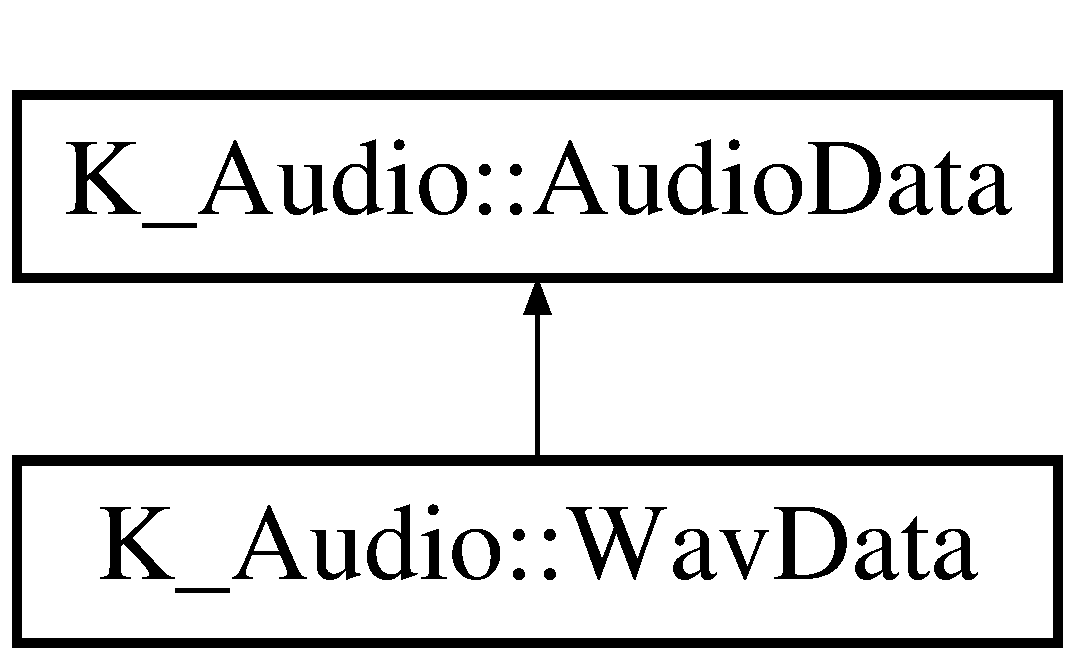
\includegraphics[height=2.000000cm]{class_k___audio_1_1_wav_data}
\end{center}
\end{figure}
\subsection*{公開メンバ関数}
\begin{DoxyCompactItemize}
\item 
\mbox{\hyperlink{class_k___audio_1_1_wav_data_aaf0c57f6c02384ceee689de4ef19cd18}{Wav\+Data}} (const char $\ast$file\+Pass)
\item 
\mbox{\hyperlink{class_k___audio_1_1_wav_data_ad05439665a69a1cc318c79d869fa97e9}{$\sim$\+Wav\+Data}} ()
\item 
void \mbox{\hyperlink{class_k___audio_1_1_wav_data_a2af2d93fb22fe25a4739c2b40526a7af}{Seek}} (int offset)
\item 
int \mbox{\hyperlink{class_k___audio_1_1_wav_data_a9b64967d83ac218c71949335d0583e69}{Read}} (char $\ast$buffer, int max\+Size)
\end{DoxyCompactItemize}
\subsection*{その他の継承メンバ}


\subsection{構築子と解体子}
\mbox{\Hypertarget{class_k___audio_1_1_wav_data_aaf0c57f6c02384ceee689de4ef19cd18}\label{class_k___audio_1_1_wav_data_aaf0c57f6c02384ceee689de4ef19cd18}} 
\index{K\+\_\+\+Audio\+::\+Wav\+Data@{K\+\_\+\+Audio\+::\+Wav\+Data}!Wav\+Data@{Wav\+Data}}
\index{Wav\+Data@{Wav\+Data}!K\+\_\+\+Audio\+::\+Wav\+Data@{K\+\_\+\+Audio\+::\+Wav\+Data}}
\subsubsection{\texorpdfstring{Wav\+Data()}{WavData()}}
{\footnotesize\ttfamily K\+\_\+\+Audio\+::\+Wav\+Data\+::\+Wav\+Data (\begin{DoxyParamCaption}\item[{const char $\ast$}]{file\+Pass }\end{DoxyParamCaption})}

\mbox{\Hypertarget{class_k___audio_1_1_wav_data_ad05439665a69a1cc318c79d869fa97e9}\label{class_k___audio_1_1_wav_data_ad05439665a69a1cc318c79d869fa97e9}} 
\index{K\+\_\+\+Audio\+::\+Wav\+Data@{K\+\_\+\+Audio\+::\+Wav\+Data}!````~Wav\+Data@{$\sim$\+Wav\+Data}}
\index{````~Wav\+Data@{$\sim$\+Wav\+Data}!K\+\_\+\+Audio\+::\+Wav\+Data@{K\+\_\+\+Audio\+::\+Wav\+Data}}
\subsubsection{\texorpdfstring{$\sim$\+Wav\+Data()}{~WavData()}}
{\footnotesize\ttfamily K\+\_\+\+Audio\+::\+Wav\+Data\+::$\sim$\+Wav\+Data (\begin{DoxyParamCaption}{ }\end{DoxyParamCaption})}



\subsection{関数詳解}
\mbox{\Hypertarget{class_k___audio_1_1_wav_data_a9b64967d83ac218c71949335d0583e69}\label{class_k___audio_1_1_wav_data_a9b64967d83ac218c71949335d0583e69}} 
\index{K\+\_\+\+Audio\+::\+Wav\+Data@{K\+\_\+\+Audio\+::\+Wav\+Data}!Read@{Read}}
\index{Read@{Read}!K\+\_\+\+Audio\+::\+Wav\+Data@{K\+\_\+\+Audio\+::\+Wav\+Data}}
\subsubsection{\texorpdfstring{Read()}{Read()}}
{\footnotesize\ttfamily int K\+\_\+\+Audio\+::\+Wav\+Data\+::\+Read (\begin{DoxyParamCaption}\item[{char $\ast$}]{buffer,  }\item[{int}]{max\+Size }\end{DoxyParamCaption})\hspace{0.3cm}{\ttfamily [virtual]}}



\mbox{\hyperlink{class_k___audio_1_1_audio_data_af42b123ad2ce45867401d697fd572392}{K\+\_\+\+Audio\+::\+Audio\+Data}}を実装しています。

\mbox{\Hypertarget{class_k___audio_1_1_wav_data_a2af2d93fb22fe25a4739c2b40526a7af}\label{class_k___audio_1_1_wav_data_a2af2d93fb22fe25a4739c2b40526a7af}} 
\index{K\+\_\+\+Audio\+::\+Wav\+Data@{K\+\_\+\+Audio\+::\+Wav\+Data}!Seek@{Seek}}
\index{Seek@{Seek}!K\+\_\+\+Audio\+::\+Wav\+Data@{K\+\_\+\+Audio\+::\+Wav\+Data}}
\subsubsection{\texorpdfstring{Seek()}{Seek()}}
{\footnotesize\ttfamily void K\+\_\+\+Audio\+::\+Wav\+Data\+::\+Seek (\begin{DoxyParamCaption}\item[{int}]{offset }\end{DoxyParamCaption})\hspace{0.3cm}{\ttfamily [virtual]}}



\mbox{\hyperlink{class_k___audio_1_1_audio_data_a1ba3ab1b4bae0b460d26278cb29ce16e}{K\+\_\+\+Audio\+::\+Audio\+Data}}を実装しています。


%--- End generated contents ---

% Index
\backmatter
\newpage
\phantomsection
\clearemptydoublepage
\addcontentsline{toc}{chapter}{索引}
\printindex

\end{document}
